\documentclass[twoside]{book}

% Packages required by doxygen
\usepackage{calc}
\usepackage{doxygen}
\usepackage{graphicx}
\usepackage[utf8]{inputenc}
\usepackage{makeidx}
\usepackage{multicol}
\usepackage{multirow}
\usepackage{textcomp}
\usepackage[table]{xcolor}

% Font selection
\usepackage[T1]{fontenc}
\usepackage{mathptmx}
\usepackage[scaled=.90]{helvet}
\usepackage{courier}
\usepackage{amssymb}
\usepackage{sectsty}
\renewcommand{\familydefault}{\sfdefault}
\allsectionsfont{%
  \fontseries{bc}\selectfont%
  \color{darkgray}%
}
\renewcommand{\DoxyLabelFont}{%
  \fontseries{bc}\selectfont%
  \color{darkgray}%
}

% Page & text layout
\usepackage{geometry}
\geometry{%
  a4paper,%
  top=2.5cm,%
  bottom=2.5cm,%
  left=2.5cm,%
  right=2.5cm%
}
\tolerance=750
\hfuzz=15pt
\hbadness=750
\setlength{\emergencystretch}{15pt}
\setlength{\parindent}{0cm}
\setlength{\parskip}{0.2cm}
\makeatletter
\renewcommand{\paragraph}{%
  \@startsection{paragraph}{4}{0ex}{-1.0ex}{1.0ex}{%
    \normalfont\normalsize\bfseries\SS@parafont%
  }%
}
\renewcommand{\subparagraph}{%
  \@startsection{subparagraph}{5}{0ex}{-1.0ex}{1.0ex}{%
    \normalfont\normalsize\bfseries\SS@subparafont%
  }%
}
\makeatother

% Headers & footers
\usepackage{fancyhdr}
\pagestyle{fancyplain}
\fancyhead[LE]{\fancyplain{}{\bfseries\thepage}}
\fancyhead[CE]{\fancyplain{}{}}
\fancyhead[RE]{\fancyplain{}{\bfseries\leftmark}}
\fancyhead[LO]{\fancyplain{}{\bfseries\rightmark}}
\fancyhead[CO]{\fancyplain{}{}}
\fancyhead[RO]{\fancyplain{}{\bfseries\thepage}}
\fancyfoot[LE]{\fancyplain{}{}}
\fancyfoot[CE]{\fancyplain{}{}}
\fancyfoot[RE]{\fancyplain{}{\bfseries\scriptsize Generated on Fri Apr 5 2019 19\-:46\-:35 for Top\-Tagger by Doxygen }}
\fancyfoot[LO]{\fancyplain{}{\bfseries\scriptsize Generated on Fri Apr 5 2019 19\-:46\-:35 for Top\-Tagger by Doxygen }}
\fancyfoot[CO]{\fancyplain{}{}}
\fancyfoot[RO]{\fancyplain{}{}}
\renewcommand{\footrulewidth}{0.4pt}
\renewcommand{\chaptermark}[1]{%
  \markboth{#1}{}%
}
\renewcommand{\sectionmark}[1]{%
  \markright{\thesection\ #1}%
}

% Indices & bibliography
\usepackage{natbib}
\usepackage[titles]{tocloft}
\setcounter{tocdepth}{3}
\setcounter{secnumdepth}{5}
\makeindex

% Hyperlinks (required, but should be loaded last)
\usepackage{ifpdf}
\ifpdf
  \usepackage[pdftex,pagebackref=true]{hyperref}
\else
  \usepackage[ps2pdf,pagebackref=true]{hyperref}
\fi
\hypersetup{%
  colorlinks=true,%
  linkcolor=blue,%
  citecolor=blue,%
  unicode%
}

% Custom commands
\newcommand{\clearemptydoublepage}{%
  \newpage{\pagestyle{empty}\cleardoublepage}%
}


%===== C O N T E N T S =====

\begin{document}

% Titlepage & ToC
\hypersetup{pageanchor=false}
\pagenumbering{roman}
\begin{titlepage}
\vspace*{7cm}
\begin{center}%
{\Large Top\-Tagger }\\
\vspace*{1cm}
{\large Generated by Doxygen 1.8.6}\\
\vspace*{0.5cm}
{\small Fri Apr 5 2019 19:46:35}\\
\end{center}
\end{titlepage}
\clearemptydoublepage
\tableofcontents
\clearemptydoublepage
\pagenumbering{arabic}
\hypersetup{pageanchor=true}

%--- Begin generated contents ---
\chapter{Top Tagger}
\label{index}\hypertarget{index}{}\section*{Top Tagging Algorithm}

Add description of algorithm and general options here

\section*{Installation Instructions}

\subsection*{Installing the tagger in C\-M\-S software release}

\subsubsection*{Standalone (edm free) install instructions within C\-M\-S\-S\-W}

These instructions explain how to install the top tagger in a standalone way (i.\-e. no cms\-Run or F\-W\-Lite required) but taking advantage of all the tools which come packaged with a C\-M\-S\-S\-W release. If you would rather not go through the hassle of installing R\-O\-O\-T/python/tensorflow, the C\-M\-S\-S\-W environment can be used to provide the necessary libraries and python modules


\begin{DoxyCode}
cmsrel CMSSW\_9\_4\_11
cd CMSSW\_9\_4\_11/src
cmsenv
git clone git@github.com:susy2015/\hyperlink{classTopTagger}{TopTagger}.git
cd \hyperlink{classTopTagger}{TopTagger}/\hyperlink{classTopTagger}{TopTagger}/test
./configure
make -j8 
\end{DoxyCode}


The test code can then be run identically to the completely standalone instructions found \href{../README.md#running-the-example}{\tt here}

\subsubsection*{Install tagger integrated in the edm framework}

These instructions explain how to install the top tagger code if you want to run the tagger during nano\-A\-O\-D production or other cms\-Run driven analysis tasks.

\paragraph*{Description of top tagger nano\-A\-O\-D format}

The tagger will save an abbreviated \hyperlink{classTopObject}{Top\-Object} for each top into the nano\-A\-O\-D. The information stored includes


\begin{DoxyCode}
nResolvedTop (\textcolor{keywordtype}{int}): The number of resolved tops in the event
ResolvedTop\_discriminator (float): The neural network discrimimnator for topness (1 is most top like, 0 is 
      least top like)
ResolvedTop\_pt (float): Pt of the top
ResolvedTop\_eta (float): Eta of the top
ResolvedTop\_phi (float): Phi of the top
ResolvedTop\_mass (float): Mass of the top
ResolvedTop\_j1Idx (int): Index of the first constituent jet in the main nanoAOD jet collection
ResolvedTop\_j2Idx (int): Index of the second constituent jet in the main nanoAOD jet collectino
ResolvedTop\_j3Idx (int): Index of the third constituent jet in the main nanoAOD jet collection
ResolvedTop\_type (int): The type of top (3 for resolved tops)
\end{DoxyCode}


In order to save space in the nano\-A\-O\-D only top objects passing a basic discriminator cut are saved.

\paragraph*{Instructions for saving tagger results to nano\-A\-O\-D with C\-M\-S\-S\-W\-\_\-9\-\_\-4\-\_\-11}

If starting from a fresh release of C\-M\-S\-S\-W run the following setup commands


\begin{DoxyCode}
\textcolor{preprocessor}{#get CMSSW release}
\textcolor{preprocessor}{}cmsrel CMSSW\_9\_4\_11
cd CMSSW\_9\_4\_11/src/
cmsenv
git cms-init
\end{DoxyCode}


The following additional packages should then be checked out to get the top tagging code and the qg\-Axis1 variable necessary for the latest versions of the tagger.


\begin{DoxyCode}
cd $\{CMSSW\_BASE\}/src
git cms-merge-topic -u pastika:AddAxis1\_946p1
git clone git@github.com:susy2015/\hyperlink{classTopTagger}{TopTagger}.git
scram b -j4
\end{DoxyCode}


The configuration file to generate nano\-A\-O\-D can then be generated with the following set of instructions via cms\-Driver.\-py and download the top tagger configuration file


\begin{DoxyCode}
cd $\{CMSSW\_BASE\}/src
cmsDriver.py test94X -s NANO --mc --eventcontent NANOAODSIM --datatier NANOAODSIM --filein [location of 
      miniAOD file] --no\_exec  --conditions \textcolor{keyword}{auto}:phase1\_2017\_realistic -n 100 --era Run2\_2017,
      run2\_nanoAOD\_94XMiniAODv1 --customise \hyperlink{classTopTagger}{TopTagger}/\hyperlink{classTopTagger}{TopTagger}/resolvedTagger\_cff.customizeResolvedTagger
mkdir -p $\{CMSSW\_BASE\}/src/\hyperlink{classTopTagger}{TopTagger}/\hyperlink{classTopTagger}{TopTagger}/data
getTaggerCfg.sh -o -n -t DeepResolved\_DeepCSV\_GR\_noDisc\_Release\_v1.0.0 -d $CMSSW\_BASE/src/
      \hyperlink{classTopTagger}{TopTagger}/\hyperlink{classTopTagger}{TopTagger}/data
\end{DoxyCode}


For running over 2016 M\-C insread use the following cms\-Driver command


\begin{DoxyCode}
cd $\{CMSSW\_BASE\}/src
cmsDriver.py test80X -s NANO --mc --eventcontent NANOAODSIM --datatier NANOAODSIM --filein [location of 
      miniAOD file] --no\_exec  --conditions \textcolor{keyword}{auto}:run2\_mc -n 100 --era Run2\_2016,run2\_miniAOD\_80XLegacy --customise 
      \hyperlink{classTopTagger}{TopTagger}/\hyperlink{classTopTagger}{TopTagger}/resolvedTagger\_cff.customizeResolvedTagger
\end{DoxyCode}


This will produce a file \char`\"{}test\mbox{[}80/94\mbox{]}\-X\-\_\-\-N\-A\-N\-O.\-py\char`\"{} which can be run as follows to produce a small test nano\-A\-O\-D file with the top tagger variables included


\begin{DoxyCode}
cmsRun test94X\_NANO.py
\end{DoxyCode}


\paragraph*{Instructions for running tagger with C\-M\-S\-S\-W 8\-\_\-0\-\_\-28\-\_\-patch1}

These instructions are not recomended. Please use the instruction above for C\-M\-S\-S\-W\-\_\-9\-\_\-4\-\_\-\-X in nano\-A\-O\-D.

In addition to the top tagger itself these instructions include the steps to configure additional packages, including the deep\-Flavor tagger (for the tagger itself along with the tensorflow configuration for 8\-X), a patch to the qg producer to produce the Axis1 variable, and a version of the jet toolbox with a minor bug fix,


\begin{DoxyCode}
\textcolor{preprocessor}{#get CMSSW release}
\textcolor{preprocessor}{}cmsrel CMSSW\_8\_0\_28\_patch1
cd CMSSW\_8\_0\_28\_patch1/src/
cmsenv
git cms-init
\textcolor{preprocessor}{#configure deep Flavor https://twiki.cern.ch/twiki/bin/viewauth/CMS/DeepJet}
\textcolor{preprocessor}{}git cms-merge-topic -u mverzett:Experimental\_DeepFlavour\_80X
cd RecoBTag/DeepFlavour/scripts/
wget -nv http:\textcolor{comment}{//www-ekp.physik.uni-karlsruhe.de/~harrendorf/tensorflow-cmssw8-0-26.tar.gz}
tar -zxf tensorflow-cmssw8-0-26.tar.gz
mv tensorflow-cmssw8-0-26-patch1/site-packages ../../Tensorflow/python
rm -rf tensorflow-cmssw8-0-26.tar.gz tensorflow-cmssw8-0-26-patch1/
cd \textcolor{stringliteral}{"$CMSSW\_BASE/src"}
scram setup \textcolor{stringliteral}{"RecoBTag/Tensorflow/py2-numpy-c-api.xml"}
cmsenv
\textcolor{preprocessor}{#patch to gq producer to add axis1}
\textcolor{preprocessor}{}git cms-merge-topic -u pastika:AddJetAxis1
\textcolor{preprocessor}{#patched version of jet toolbox}
\textcolor{preprocessor}{}git clone git@github.com:susy2015/JetToolbox.git JMEAnalysis/JetToolbox -b fix\_NoLep\_jetToolbox\_80X\_V3
\textcolor{preprocessor}{#download top tagger code }
\textcolor{preprocessor}{}git clone -b IntermediateRecipeV0 git@github.com:susy2015/\hyperlink{classTopTagger}{TopTagger}.git
\textcolor{preprocessor}{#compile everything }
\textcolor{preprocessor}{}scram b -j12
cd \hyperlink{classTopTagger}{TopTagger}/\hyperlink{classTopTagger}{TopTagger}/test
\textcolor{preprocessor}{#get qgl database file}
\textcolor{preprocessor}{}wget https:\textcolor{comment}{//raw.githubusercontent.com/cms-jet/QGLDatabase/master/SQLiteFiles/QGL\_cmssw8020\_v2.db}
\textcolor{preprocessor}{#get top tager cfg file and MVA model files }
\textcolor{preprocessor}{}../../Tools/getTaggerCfg.sh -t Intermediate\_Example\_v1.0.0
\textcolor{preprocessor}{#run example code}
\textcolor{preprocessor}{}voms-proxy-init
cmsRun run\_topTagger.py
\end{DoxyCode}


The default configuration of the example cfg file \char`\"{}run\-\_\-top\-Tagger.\-py\char`\"{} will run over a single-\/lepton ttbar sample and produce an edm formatted output file (\char`\"{}test.\-root\char`\"{}) containing the vector of reconstructed top T\-Lorentz\-Vectors along with a second vector indicating the type of top (monojet, dijet, trijet).

\subsubsection*{Instructions for producing jet variables for resolved top tagger in nano\-A\-O\-D}

The configuration file to generate nano\-A\-O\-D with top tagger variables can be generated with the following set of instructions via cms\-Driver.\-py


\begin{DoxyCode}
cd $\{CMSSW\_BASE\}/src
cmsDriver.py resolvedTaggerVariables -s NANO --mc --eventcontent NANOAODSIM --datatier NANOAODSIM --filein 
      [location of miniAOD file] --no\_exec  --conditions \textcolor{keyword}{auto}:phase1\_2017\_realistic -n 100 --era Run2\_2017,
      run2\_nanoAOD\_94XMiniAODv1 --customise \hyperlink{classTopTagger}{TopTagger}/\hyperlink{classTopTagger}{TopTagger}/resolvedTagger\_cff.
      customizeResolvedTaggerVariables
mkdir -p $\{CMSSW\_BASE\}/src/\hyperlink{classTopTagger}{TopTagger}/\hyperlink{classTopTagger}{TopTagger}/data
getTaggerCfg.sh -o -n -t DeepResolved\_DeepCSV\_GR\_noDisc\_Release\_v1.0.0 -d $CMSSW\_BASE/src/
      \hyperlink{classTopTagger}{TopTagger}/\hyperlink{classTopTagger}{TopTagger}/data
\end{DoxyCode}


\subsubsection*{O\-L\-D\-: Instructions for producing jet variables for resolved top tagger in C\-M\-S\-S\-W\-\_\-8\-\_\-0\-\_\-28\-\_\-patch1}

The solution using nano\-A\-O\-D is the recomended way to get resolved top tagger variables.

Setting up a new C\-M\-S\-S\-W 8\-\_\-0\-\_\-28\-\_\-patch1 release to produce the resolved top tagger variables.


\begin{DoxyCode}
\textcolor{preprocessor}{#get CMSSW release}
\textcolor{preprocessor}{}cmsrel CMSSW\_8\_0\_28\_patch1
cd CMSSW\_8\_0\_28\_patch1/src/
\textcolor{preprocessor}{#initialize cms and cms git commands }
\textcolor{preprocessor}{}cmsenv
git cms-init
\textcolor{preprocessor}{#patch to qg producer to add axis1}
\textcolor{preprocessor}{}git cms-merge-topic -u pastika:AddJetAxis1
\textcolor{preprocessor}{#compile}
\textcolor{preprocessor}{scram b -j8}
\end{DoxyCode}


The following code should be added to your C\-M\-S\-S\-W config file to prepare the jet collection with all necessary variables.


\begin{DoxyCode}
jetTag = cms.InputTag(\textcolor{stringliteral}{"slimmedJets"})

process.load(\textcolor{stringliteral}{'RecoJets.JetProducers.QGTagger\_cfi'})
process.QGTagger.srcJets   = cms.InputTag(\textcolor{stringliteral}{"slimmedJets"})

from PhysicsTools.PatAlgos.tools.jetTools \textcolor{keyword}{import} updateJetCollection

updateJetCollection(
   process,
   labelName = \textcolor{stringliteral}{"DeepCSV"},
   jetSource = cms.InputTag(\textcolor{stringliteral}{"slimmedJets"}),
   jetCorrections = (\textcolor{stringliteral}{'AK4PFchs'}, cms.vstring([\textcolor{stringliteral}{'L1FastJet'}, \textcolor{stringliteral}{'L2Relative'}, \textcolor{stringliteral}{'L3Absolute'}]), \textcolor{stringliteral}{'None'}),
   btagDiscriminators = [
      \textcolor{stringliteral}{'pfDeepCSVJetTags:probudsg'},
      \textcolor{stringliteral}{'pfDeepCSVJetTags:probb'},
      \textcolor{stringliteral}{'pfDeepCSVJetTags:probc'},
      \textcolor{stringliteral}{'pfDeepCSVJetTags:probbb'},
      \textcolor{stringliteral}{'pfDeepCSVJetTags:probcc'},
      ] ## to add discriminators                                                                           
                                                                                                                  
                             
)

process.updatedPatJetsDeepCSV.userData.userFloats.src += [\textcolor{stringliteral}{'QGTagger:qgLikelihood'}, \textcolor{stringliteral}{'QGTagger:ptD'}, \textcolor{stringliteral}{'
      QGTagger:axis1'}, \textcolor{stringliteral}{'QGTagger:axis2'},]
process.updatedPatJetsDeepCSV.userData.userInts.src += [\textcolor{stringliteral}{'QGTagger:mult'},]
\end{DoxyCode}


This will produce a jet collection called 'selected\-Updated\-Pat\-Jets\-Deep\-C\-S\-V' which contains all necessary variables for the resolved top tagger.

The necessary variables can then be accessed in a edm producer as follows


\begin{DoxyCode}
\{c++\}
\textcolor{comment}{//in constructor}
JetTok\_ = consumes<std::vector<pat::Jet> >(edm::InputTag(\textcolor{stringliteral}{"selectedUpdatedPatJetsDeepCSV"}));
\end{DoxyCode}



\begin{DoxyCode}
\{c++\}
\textcolor{comment}{//in produce(...)}
edm::Handle<std::vector<pat::Jet> > jets;
iEvent.getByToken(JetTok\_, jets);

\textcolor{keywordflow}{for}(\textcolor{keyword}{const} pat::Jet& jet : *jets)
\{
    \textcolor{comment}{//No need to keep jets below 20 GeV}
    \textcolor{keywordflow}{if}(jet.pt() < 20) \textcolor{keywordflow}{continue};

    TLorentzVector perJetLVec;
    perJetLVec.SetPtEtaPhiE( jet.pt(), jet.eta(), jet.phi(), jet.energy() );

    \textcolor{keywordtype}{double} qgPtD = jet.userFloat(\textcolor{stringliteral}{"QGTagger:ptD"});
    \textcolor{keywordtype}{double} qgAxis1 = jet.userFloat(\textcolor{stringliteral}{"QGTagger:axis1"});
    \textcolor{keywordtype}{double} qgAxis2 = jet.userFloat(\textcolor{stringliteral}{"QGTagger:axis2"});
    \textcolor{keywordtype}{double} qgMult = \textcolor{keyword}{static\_cast<}\textcolor{keywordtype}{double}\textcolor{keyword}{>}(jet.userInt(\textcolor{stringliteral}{"QGTagger:mult"}));
    \textcolor{keywordtype}{double} deepCSVb = jet.bDiscriminator(\textcolor{stringliteral}{"pfDeepCSVJetTags:probb"});
    \textcolor{keywordtype}{double} deepCSVc = jet.bDiscriminator(\textcolor{stringliteral}{"pfDeepCSVJetTags:probc"});
    \textcolor{keywordtype}{double} deepCSVl = jet.bDiscriminator(\textcolor{stringliteral}{"pfDeepCSVJetTags:probudsg"});
    \textcolor{keywordtype}{double} deepCSVbb = jet.bDiscriminator(\textcolor{stringliteral}{"pfDeepCSVJetTags:probbb"});
    \textcolor{keywordtype}{double} deepCSVcc = jet.bDiscriminator(\textcolor{stringliteral}{"pfDeepCSVJetTags:probcc"});
    \textcolor{keywordtype}{double} btag = jet.bDiscriminator(\textcolor{stringliteral}{"pfCombinedInclusiveSecondaryVertexV2BJetTags"});
    \textcolor{keywordtype}{double} chargedHadronEnergyFraction = jet.chargedHadronEnergyFraction();
    \textcolor{keywordtype}{double} neutralHadronEnergyFraction = jet.neutralHadronEnergyFraction();
    \textcolor{keywordtype}{double} chargedEmEnergyFraction = jet.chargedEmEnergyFraction();
    \textcolor{keywordtype}{double} neutralEmEnergyFraction = jet.neutralEmEnergyFraction();
    \textcolor{keywordtype}{double} muonEnergyFraction = jet.muonEnergyFraction();
    \textcolor{keywordtype}{double} photonEnergyFraction = jet.photonEnergyFraction();
    \textcolor{keywordtype}{double} electronEnergyFraction = jet.electronEnergyFraction();
    \textcolor{keywordtype}{double} recoJetsHFHadronEnergyFraction = jet.HFHadronEnergyFraction();
    \textcolor{keywordtype}{double} recoJetsHFEMEnergyFraction = jet.HFEMEnergyFraction();
    \textcolor{keywordtype}{double} chargedHadronMultiplicity = jet.chargedHadronMultiplicity();
    \textcolor{keywordtype}{double} neutralHadronMultiplicity = jet.neutralHadronMultiplicity();
    \textcolor{keywordtype}{double} photonMultiplicity = jet.photonMultiplicity();
    \textcolor{keywordtype}{double} electronMultiplicity = jet.electronMultiplicity();
    \textcolor{keywordtype}{double} muonMultiplicity = jet.muonMultiplicity();
\}
\end{DoxyCode}


For convinenent use with the top tagger the 4-\/vector and each jet variable can be saved in a flat tuple in its own std\-::vector per event.

\subsection*{More about getting a configuration file}

Before the top tagger can be used the top tagger configuration file must be checked out. Configuration files for top tagger working points are stored in the Susy2015/\-Top\-Tagger\-Cfg repository and are published through releases. These should not be accessed directly, but instead you can use the script \char`\"{}get\-Tagger\-Cfg.\-sh\char`\"{} to download the working points desired. An example of a basic checkout of the standard working point for use with the example code (different working points are found here \href{https://github.com/susy2015/TopTaggerCfg/releases}{\tt https\-://github.\-com/susy2015/\-Top\-Tagger\-Cfg/releases}) is as follows


\begin{DoxyCode}
\textcolor{preprocessor}{#run the following once to set up the top tagger and add the "getTaggerCfg.sh" to the path}
\textcolor{preprocessor}{}source \hyperlink{classTopTagger}{TopTagger}/\hyperlink{classTopTagger}{TopTagger}/test/taggerSetup.sh
getTaggerCfg.sh -t MVAAK8\_Tight\_noQGL\_binaryCSV\_v1.0.2
\end{DoxyCode}


This will download the configuration file along with the M\-V\-A training file if appropriate into a directory. It will then softlink the files into your current directory so this script is intended to be run from the same directory as you will run your code. If you want the directory containing the configuration file and M\-V\-A file to be located elsewhere this can be specified with the \char`\"{}-\/d\char`\"{} option (Multiple run directories can point to the same directory, this can be helpful to save space as the random forest training files are quite large). If you have multiple configuration files you can specify a different name for the configuration file with the \char`\"{}-\/f\char`\"{} option. Finally, if you want to download the file without creating the softlinks use the \char`\"{}-\/n\char`\"{} option.

\subsection*{Top tagger structure}

The top tagger code is written to take modules which act on a central object to produce the final collection of top objects. The tagger framework consists of the following classes (found in Top\-Tagger/\-Top\-Tagger/)

\subsubsection*{Top Tagger Modules and the Configuration File.}

The configuration file is central to the functioning of the top tagger code. This file is a basic text file implemented to follow the structure of the H\-C\-A\-L configuration parser and the code can be found here \char`\"{}\-Top\-Tagger/\-Cfg\-Parser.\char`\"{} This code upon which this is based can be found here (\href{https://svnweb.cern.ch/cern/wsvn/cmshcos/trunk/hcalBase/include/hcal/cfg/?#aafaf15fcace155f9a3d702b52eb6d719}{\tt https\-://svnweb.\-cern.\-ch/cern/wsvn/cmshcos/trunk/hcal\-Base/include/hcal/cfg/?\#aafaf15fcace155f9a3d702b52eb6d719}). The configuration script is used to tell the top tagger what modules to run and in which order, in addition to allowing any parameters necessary for the tagger and each module to be defined cleanly in one place. An example configuration script can be found in Top\-Tagger/\-Top\-Tagger/test/\-Example\-\_\-\-Top\-Tagger.\-cfg

Modules are where all the real work of the top tagger is done. Each module performs a particular task and stores its results in a \hyperlink{classTopTaggerResults}{Top\-Tagger\-Results} object which will eventually be presented to the user as a summary of final results. All modules inherit from \hyperlink{classTTModule}{T\-T\-Module} and, as described in \hyperlink{classTTModule}{T\-T\-Module}\char`\"{} implement the 2 functions \char`\"{}get\-Parameter\char`\"{}s and \char`\"{}run." Each module is called automatically from the \hyperlink{classTopTagger}{Top\-Tagger} class. They are also instantiated automatically based upon the configuration file.

For further documentation of the code and each module see the following webpage \href{http://susy2015.github.io/TopTagger/html/index.html}{\tt http\-://susy2015.\-github.\-io/\-Top\-Tagger/html/index.\-html}.

\subsubsection*{\hyperlink{classTopTagger}{Top\-Tagger}}

The \hyperlink{classTopTagger}{Top\-Tagger} module is the primary (and only mandatory) section in every top tagger configuration. This section defines all the other top tagger modules which will be run and in which order. This module has 2 variables (both arrays) Which are used to define the module run order and if necessary the module context name.

\paragraph*{module\mbox{[}\mbox{]} (string)\-:}

This variable is an array and is used to define which other modules will be run and in which order. This can be any module listed here in this section.

\paragraph*{context\mbox{[}\mbox{]} (string)\-:}

This variable must be specified for any module being run more than once to specify what context name to read its configuration from. 
\chapter{Top\-Tagger}
\label{md__home_travis_build_susy2015_TopTagger_README}
\hypertarget{md__home_travis_build_susy2015_TopTagger_README}{}
\subsection*{Standalone installation instructions}

\subsubsection*{Installing prerequisites}

To compile the standalone library requires the R\-O\-O\-T 6 \mbox{[}1\mbox{]} and Tensorflow 1.\-2 (or newer) \mbox{[}2\mbox{]} packages.

\mbox{[}1\mbox{]} \href{https://root.cern.ch/downloading-root}{\tt https\-://root.\-cern.\-ch/downloading-\/root}

Follow the instructions to install R\-O\-O\-T on your system

\mbox{[}2\mbox{]} \href{https://www.tensorflow.org/install/install_c}{\tt https\-://www.\-tensorflow.\-org/install/install\-\_\-c}

Follow the instructions to install tensorflow for C. G\-P\-U support is not necessary unless you will be training new models. For compatibility with the \hyperlink{classTopTagger}{Top\-Tagger} model run the following download command in place of step 2 on this page to download tensorflow v1.\-3.\-0 instead of the lastest version


\begin{DoxyCode}
TF\_TYPE=\textcolor{stringliteral}{"cpu"} # Change to \textcolor{stringliteral}{"gpu"} \textcolor{keywordflow}{for} GPU support (not necessary \textcolor{keywordflow}{for} inferance)
OS=\textcolor{stringliteral}{"linux"} # Change to \textcolor{stringliteral}{"darwin"} \textcolor{keywordflow}{for} macOS
TARGET\_DIRECTORY=\textcolor{stringliteral}{"/usr/local"}  #Change \textcolor{keyword}{this} to install the c-api in other places 
curl -L \(\backslash\)
  \textcolor{stringliteral}{"
      https://storage.googleapis.com/tensorflow/libtensorflow/libtensorflow-$\{TF\_TYPE\}-$\{OS\}-x86\_64-1.3.0.tar.gz"} |
  sudo tar -C $TARGET\_DIRECTORY -xz
\end{DoxyCode}


\subsubsection*{Compiling the top tagger}

After all the necessary packages are installed, checkout the \hyperlink{classTopTagger}{Top\-Tagger} repository and compile with the following command (with a terminal configured to use root/tensorflow)


\begin{DoxyCode}
\textcolor{preprocessor}{#After downloading the code from github or untaring the standalone tarball }
\textcolor{preprocessor}{}cd \hyperlink{classTopTagger}{TopTagger}/\hyperlink{classTopTagger}{TopTagger}/test
./configure
make -j4
\textcolor{preprocessor}{#To install in a non-standard directory add PREFIX=/install/path to the configure command}
\textcolor{preprocessor}{}\textcolor{preprocessor}{#If the tensorflow c-api was installed elsewhere than "/usr/local" add TENSORFLOWPATH=[path to c-api] to
       the configure command}
\textcolor{preprocessor}{}\textcolor{preprocessor}{#the command below is optional for system wide install (will require sudo rights)}
\textcolor{preprocessor}{make install}
\end{DoxyCode}


This command will produce a static and a shared library which contain all the necessary symbols to link the top tagger into other C++ code. This will also compile a standalone example called ``top\-Tagger\-Test''.

\subsection*{Example code}

A basic standalone example using the top tagging code is provided in \char`\"{}\-Top\-Tagger/test/top\-Tagger\-Test.\-cpp\char`\"{}. This is a basic example program which reads in the necessary top tagger inputs from a file (``example\-Inputs.root'') and runs the top tagger code. As validation, this prints out the number of top quarks reconstructed in each event as well as some basic properties of each top quark reconstructed. For reference the output of this script can be seen at the end of this readme.

\subsubsection*{Running the example}

The example executable is compiled along with the standalone library as described above. If the top tagger was not installed system wide, then there is a script \char`\"{}tagger\-Setup.\-sh\char`\"{} which is produced by the configure command which must be sourced to set system variables appropriately. A \char`\"{}.\-csh\char`\"{} version is also proveded"


\begin{DoxyCode}
\textcolor{preprocessor}{#do once per terminal if opencv or the top tagger are not installed system wide}
\textcolor{preprocessor}{}source taggerSetup.sh
\textcolor{preprocessor}{#do once in any directory where you will run the top tagger example}
\textcolor{preprocessor}{}getTaggerCfg.sh -t DeepCombined\_Example\_v1.0.1
\textcolor{preprocessor}{#run the example code}
\textcolor{preprocessor}{./topTaggerTest}
\end{DoxyCode}


\subsubsection*{Tagger input variables}

The top tagging algorithm takes both a collection of all A\-K4 jets and all A\-K8 jets (passing basic pt and $\vert$eta$\vert$ acceptance requirments) along with supporting variables. The input variables used for the example program are listed below


\begin{DoxyCode}
\textcolor{comment}{//Variables to hold inputs}
\textcolor{comment}{//AK4 jet variables}
\textcolor{comment}{//Each entry in these vectors refers to information for 1 AK4 jet}
std::vector<TLorentzVector>** AK4JetLV = \textcolor{keyword}{new} std::vector<TLorentzVector>*();
std::vector<double>** AK4JetBtag = \textcolor{keyword}{new} std::vector<double>*();
std::vector<double>** AK4qgMult = \textcolor{keyword}{new} std::vector<double>*();
std::vector<double>** AK4qgPtD = \textcolor{keyword}{new} std::vector<double>*();
std::vector<double>** AK4qgAxis1 = \textcolor{keyword}{new} std::vector<double>*();
std::vector<double>** AK4qgAxis2 = \textcolor{keyword}{new} std::vector<double>*();
std::vector<double>** AK4recoJetschargedHadronEnergyFraction = \textcolor{keyword}{new} std::vector<double>*();
std::vector<double>** AK4recoJetschargedEmEnergyFraction = \textcolor{keyword}{new} std::vector<double>*();
std::vector<double>** AK4recoJetsneutralEmEnergyFraction = \textcolor{keyword}{new} std::vector<double>*();
std::vector<double>** AK4ElectronEnergyFraction = \textcolor{keyword}{new} std::vector<double>*();
std::vector<double>** AK4PhotonEnergyFraction = \textcolor{keyword}{new} std::vector<double>*();
std::vector<double>** AK4recoJetsneutralEnergyFraction = \textcolor{keyword}{new} std::vector<double>*();
std::vector<double>** AK4recoJetsHFHadronEnergyFraction = \textcolor{keyword}{new} std::vector<double>*();
std::vector<double>** AK4recoJetsmuonEnergyFraction = \textcolor{keyword}{new} std::vector<double>*();
std::vector<double>** AK4recoJetsHFEMEnergyFraction = \textcolor{keyword}{new} std::vector<double>*();
std::vector<double>** AK4NeutralHadronMultiplicity = \textcolor{keyword}{new} std::vector<double>*();
std::vector<double>** AK4ChargedHadronMultiplicity = \textcolor{keyword}{new} std::vector<double>*();
std::vector<double>** AK4ElectronMultiplicity = \textcolor{keyword}{new} std::vector<double>*();
std::vector<double>** AK4MuonMultiplicity = \textcolor{keyword}{new} std::vector<double>*();
std::vector<double>** AK4PhotonMultiplicity = \textcolor{keyword}{new} std::vector<double>*();
std::vector<double>** AK4DeepCSVbb = \textcolor{keyword}{new} std::vector<double>*();
std::vector<double>** AK4DeepCSVb = \textcolor{keyword}{new} std::vector<double>*();
std::vector<double>** AK4DeepCSVc = \textcolor{keyword}{new} std::vector<double>*();
std::vector<double>** AK4DeepCSVcc = \textcolor{keyword}{new} std::vector<double>*();

\textcolor{comment}{//AK8 jet varaibles}
\textcolor{comment}{//The elements of each vector refer to one AK8 jet}
std::vector<TLorentzVector>** AK8JetLV = \textcolor{keyword}{new} std::vector<TLorentzVector>*();
std::vector<double>** AK8JetTau1 = \textcolor{keyword}{new} std::vector<double>*();
std::vector<double>** AK8JetTau2 = \textcolor{keyword}{new} std::vector<double>*();
std::vector<double>** AK8JetTau3 = \textcolor{keyword}{new} std::vector<double>*();
std::vector<double>** AK8JetSoftdropMass = \textcolor{keyword}{new} std::vector<double>*();
std::vector<std::vector<TLorentzVector>>** AK8SubjetLV = \textcolor{keyword}{new} std::vector<std::vector<TLorentzVector>>*();
std::vector<std::vector<double>>** AK8SubjetBtag  = \textcolor{keyword}{new} std::vector<std::vector<double>>*();
std::vector<std::vector<double>>** AK8SubjetMult  = \textcolor{keyword}{new} std::vector<std::vector<double>>*();
std::vector<std::vector<double>>** AK8SubjetPtD   = \textcolor{keyword}{new} std::vector<std::vector<double>>*();
std::vector<std::vector<double>>** AK8SubjetAxis1 = \textcolor{keyword}{new} std::vector<std::vector<double>>*();
std::vector<std::vector<double>>** AK8SubjetAxis2 = \textcolor{keyword}{new} std::vector<std::vector<double>>*();
\end{DoxyCode}


\subsubsection*{Output of example code}

In addition to the code output below you may also get some tensorflow warnings about tensorflow not being compiled to tsupport various special C\-P\-U instruction sets. This is ok and these messages can be ignored.


\begin{DoxyCode}
--- Reader                   : Booking \textcolor{stringliteral}{"BDTG"} of type \textcolor{stringliteral}{"BDT"} from weights-t2tt850-sm-baseline-nodphi-nomtb-
      hqu-08112016.xml.
--- MethodBase               : Reading weight file: weights-t2tt850-sm-baseline-nodphi-nomtb-hqu-08112016.
      xml
--- BDTG                     : Read method \textcolor{stringliteral}{"BDTG"} of type \textcolor{stringliteral}{"BDT"}
--- BDTG                     : MVA method was trained with TMVA Version: 4.2.1
--- BDTG                     : MVA method was trained with ROOT Version: 6.06/08
--- DataSetInfo              : Added \textcolor{keyword}{class }"Signal"    with internal class number 0
--- DataSetInfo              : Added class "Background"      with internal class number 1
--- Reader                   : Booked classifier "BDTG" of type: "BDT"
--- Reader                   : Booking "BDTG" of type "BDT" from sdWTag\_ttbarTraining\_v0.xml.
--- MethodBase               : Reading weight file: sdWTag\_ttbarTraining\_v0.xml
--- BDTG                     : Read method "BDTG" of type "BDT"
--- BDTG                     : MVA method was trained with TMVA Version: 4.2.1
--- BDTG                     : MVA method was trained with ROOT Version: 6.06/02
--- DataSetInfo              : Added class "Signal"    with internal class number 0
--- DataSetInfo              : Added class "Background"      with internal class number 1
--- Reader                   : Booked classifier "BDTG" of type: "BDT"
Event #: 1
      N tops: 1
      Top properties: N constituents:   3,   Pt:  436.5,   Eta:   1.398,   Phi:  -2.267
          \hyperlink{classConstituent}{Constituent} properties: \hyperlink{classConstituent}{Constituent} type:   1,   Pt:  227.8,   Eta:   1.278
      ,   Phi:  -2.403
          \hyperlink{classConstituent}{Constituent} properties: \hyperlink{classConstituent}{Constituent} type:   1,   Pt:  157.5,   Eta:   1.708
      ,   Phi:  -2.060
          \hyperlink{classConstituent}{Constituent} properties: \hyperlink{classConstituent}{Constituent} type:   1,   Pt:   56.7,   Eta:   0.547
      ,   Phi:  -2.300

Event #: 2
      N tops: 2
      Top properties: N constituents:   3,   Pt:  474.9,   Eta:   1.177,   Phi:   1.374
          \hyperlink{classConstituent}{Constituent} properties: \hyperlink{classConstituent}{Constituent} type:   1,   Pt:  337.1,   Eta:   1.151
      ,   Phi:   1.275
          \hyperlink{classConstituent}{Constituent} properties: \hyperlink{classConstituent}{Constituent} type:   1,   Pt:   90.4,   Eta:   1.486
      ,   Phi:   1.778
          \hyperlink{classConstituent}{Constituent} properties: \hyperlink{classConstituent}{Constituent} type:   1,   Pt:   56.4,   Eta:   0.484
      ,   Phi:   1.334
      Top properties: N constituents:   3,   Pt:  272.0,   Eta:   0.053,   Phi:  -0.078
          \hyperlink{classConstituent}{Constituent} properties: \hyperlink{classConstituent}{Constituent} type:   1,   Pt:  210.2,   Eta:  -0.008
      ,   Phi:   0.092
          \hyperlink{classConstituent}{Constituent} properties: \hyperlink{classConstituent}{Constituent} type:   1,   Pt:   63.0,   Eta:   0.602
      ,   Phi:  -0.334
          \hyperlink{classConstituent}{Constituent} properties: \hyperlink{classConstituent}{Constituent} type:   1,   Pt:   20.0,   Eta:  -1.014
      ,   Phi:  -1.451

Event #: 3
      N tops: 0

Event #: 4
      N tops: 1
      Top properties: N constituents:   3,   Pt:  222.1,   Eta:  -0.617,   Phi:  -2.966
          \hyperlink{classConstituent}{Constituent} properties: \hyperlink{classConstituent}{Constituent} type:   1,   Pt:   87.0,   Eta:   0.195
      ,   Phi:  -2.245
          \hyperlink{classConstituent}{Constituent} properties: \hyperlink{classConstituent}{Constituent} type:   1,   Pt:   86.7,   Eta:  -0.302
      ,   Phi:   2.751
          \hyperlink{classConstituent}{Constituent} properties: \hyperlink{classConstituent}{Constituent} type:   1,   Pt:   84.2,   Eta:  -1.258
      ,   Phi:  -3.096

Event #: 5
      N tops: 1
      Top properties: N constituents:   3,   Pt:  223.0,   Eta:  -0.556,   Phi:  -1.532
          \hyperlink{classConstituent}{Constituent} properties: \hyperlink{classConstituent}{Constituent} type:   1,   Pt:  135.7,   Eta:  -0.938
      ,   Phi:  -1.428
          \hyperlink{classConstituent}{Constituent} properties: \hyperlink{classConstituent}{Constituent} type:   1,   Pt:   57.7,   Eta:  -0.136
      ,   Phi:  -1.023
          \hyperlink{classConstituent}{Constituent} properties: \hyperlink{classConstituent}{Constituent} type:   1,   Pt:   56.5,   Eta:   0.418
      ,   Phi:  -2.376

Event #: 6
      N tops: 1
      Top properties: N constituents:   1,   Pt:  628.1,   Eta:  -0.831,   Phi:   2.056
          \hyperlink{classConstituent}{Constituent} properties: \hyperlink{classConstituent}{Constituent} type:   3,   Pt:  628.1,   Eta:  -0.831
      ,   Phi:   2.056

Event #: 7
      N tops: 0

Event #: 8
      N tops: 1
      Top properties: N constituents:   3,   Pt:  424.4,   Eta:   0.958,   Phi:   2.787
          \hyperlink{classConstituent}{Constituent} properties: \hyperlink{classConstituent}{Constituent} type:   1,   Pt:  261.0,   Eta:   0.838
      ,   Phi:   2.855
          \hyperlink{classConstituent}{Constituent} properties: \hyperlink{classConstituent}{Constituent} type:   1,   Pt:  128.4,   Eta:   1.153
      ,   Phi:   2.411
          \hyperlink{classConstituent}{Constituent} properties: \hyperlink{classConstituent}{Constituent} type:   1,   Pt:   53.4,   Eta:   0.738
      ,   Phi:  -2.913

Event #: 9
      N tops: 0

Event #: 10
      N tops: 1
      Top properties: N constituents:   3,   Pt:  414.0,   Eta:  -0.250,   Phi:  -2.257
          \hyperlink{classConstituent}{Constituent} properties: \hyperlink{classConstituent}{Constituent} type:   1,   Pt:  256.7,   Eta:  -0.340
      ,   Phi:  -2.015
          \hyperlink{classConstituent}{Constituent} properties: \hyperlink{classConstituent}{Constituent} type:   1,   Pt:  135.9,   Eta:   0.088
      ,   Phi:  -2.681
          \hyperlink{classConstituent}{Constituent} properties: \hyperlink{classConstituent}{Constituent} type:   1,   Pt:   41.4,   Eta:  -0.626
      ,   Phi:  -2.398

Event #: 11
      N tops: 1
      Top properties: N constituents:   3,   Pt:  444.4,   Eta:  -0.569,   Phi:   3.114
          \hyperlink{classConstituent}{Constituent} properties: \hyperlink{classConstituent}{Constituent} type:   1,   Pt:  367.1,   Eta:  -0.500
      ,   Phi:   2.977
          \hyperlink{classConstituent}{Constituent} properties: \hyperlink{classConstituent}{Constituent} type:   1,   Pt:   73.6,   Eta:  -0.889
      ,   Phi:  -2.445
          \hyperlink{classConstituent}{Constituent} properties: \hyperlink{classConstituent}{Constituent} type:   1,   Pt:   25.6,   Eta:  -0.055
      ,   Phi:  -3.127

Event #: 12
      N tops: 1
      Top properties: N constituents:   3,   Pt:  180.0,   Eta:  -0.287,   Phi:   1.145
          \hyperlink{classConstituent}{Constituent} properties: \hyperlink{classConstituent}{Constituent} type:   1,   Pt:  141.7,   Eta:  -0.229
      ,   Phi:   1.437
          \hyperlink{classConstituent}{Constituent} properties: \hyperlink{classConstituent}{Constituent} type:   1,   Pt:   37.9,   Eta:  -0.010
      ,   Phi:   0.887
          \hyperlink{classConstituent}{Constituent} properties: \hyperlink{classConstituent}{Constituent} type:   1,   Pt:   32.0,   Eta:  -0.569
      ,   Phi:  -0.184

Event #: 13
      N tops: 1
      Top properties: N constituents:   3,   Pt:  212.3,   Eta:   0.297,   Phi:  -1.735
          \hyperlink{classConstituent}{Constituent} properties: \hyperlink{classConstituent}{Constituent} type:   1,   Pt:  172.2,   Eta:   0.249
      ,   Phi:  -1.297
          \hyperlink{classConstituent}{Constituent} properties: \hyperlink{classConstituent}{Constituent} type:   1,   Pt:   54.2,   Eta:  -0.497
      ,   Phi:  -2.536
          \hyperlink{classConstituent}{Constituent} properties: \hyperlink{classConstituent}{Constituent} type:   1,   Pt:   38.9,   Eta:   1.049
      ,   Phi:  -2.805

Event #: 14
      N tops: 1
      Top properties: N constituents:   3,   Pt:  164.5,   Eta:   1.983,   Phi:  -2.734
          \hyperlink{classConstituent}{Constituent} properties: \hyperlink{classConstituent}{Constituent} type:   1,   Pt:  135.4,   Eta:   1.743
      ,   Phi:  -2.528
          \hyperlink{classConstituent}{Constituent} properties: \hyperlink{classConstituent}{Constituent} type:   1,   Pt:   48.5,   Eta:   1.023
      ,   Phi:  -2.983
          \hyperlink{classConstituent}{Constituent} properties: \hyperlink{classConstituent}{Constituent} type:   1,   Pt:   21.8,   Eta:   2.641
      ,   Phi:   1.216

Event #: 15
      N tops: 0

Event #: 16
      N tops: 2
      Top properties: N constituents:   3,   Pt:  232.8,   Eta:   0.381,   Phi:  -2.796
          \hyperlink{classConstituent}{Constituent} properties: \hyperlink{classConstituent}{Constituent} type:   1,   Pt:  218.7,   Eta:   0.454
      ,   Phi:  -2.650
          \hyperlink{classConstituent}{Constituent} properties: \hyperlink{classConstituent}{Constituent} type:   1,   Pt:   43.7,   Eta:  -0.260
      ,   Phi:   1.801
          \hyperlink{classConstituent}{Constituent} properties: \hyperlink{classConstituent}{Constituent} type:   1,   Pt:   24.4,   Eta:  -0.025
      ,   Phi:  -2.305
      Top properties: N constituents:   3,   Pt:  219.0,   Eta:  -0.721,   Phi:  -1.208
          \hyperlink{classConstituent}{Constituent} properties: \hyperlink{classConstituent}{Constituent} type:   1,   Pt:  165.8,   Eta:  -0.590
      ,   Phi:  -1.427
          \hyperlink{classConstituent}{Constituent} properties: \hyperlink{classConstituent}{Constituent} type:   1,   Pt:   54.8,   Eta:  -0.675
      ,   Phi:  -0.903
          \hyperlink{classConstituent}{Constituent} properties: \hyperlink{classConstituent}{Constituent} type:   1,   Pt:   20.3,   Eta:  -1.137
      ,   Phi:   0.122

Event #: 17
      N tops: 2
      Top properties: N constituents:   3,   Pt:  332.1,   Eta:  -0.661,   Phi:  -1.792
          \hyperlink{classConstituent}{Constituent} properties: \hyperlink{classConstituent}{Constituent} type:   1,   Pt:  172.8,   Eta:  -0.978
      ,   Phi:  -1.621
          \hyperlink{classConstituent}{Constituent} properties: \hyperlink{classConstituent}{Constituent} type:   1,   Pt:  110.1,   Eta:  -0.073
      ,   Phi:  -2.054
          \hyperlink{classConstituent}{Constituent} properties: \hyperlink{classConstituent}{Constituent} type:   1,   Pt:   55.5,   Eta:  -0.524
      ,   Phi:  -1.810
      Top properties: N constituents:   3,   Pt:  194.3,   Eta:  -1.203,   Phi:   2.916
          \hyperlink{classConstituent}{Constituent} properties: \hyperlink{classConstituent}{Constituent} type:   1,   Pt:  157.4,   Eta:  -0.889
      ,   Phi:   2.990
          \hyperlink{classConstituent}{Constituent} properties: \hyperlink{classConstituent}{Constituent} type:   1,   Pt:   36.0,   Eta:  -1.900
      ,   Phi:  -3.015
          \hyperlink{classConstituent}{Constituent} properties: \hyperlink{classConstituent}{Constituent} type:   1,   Pt:   24.3,   Eta:  -0.674
      ,   Phi:   1.492

Event #: 18
      N tops: 1
      Top properties: N constituents:   3,   Pt:  272.1,   Eta:   0.708,   Phi:   0.539
          \hyperlink{classConstituent}{Constituent} properties: \hyperlink{classConstituent}{Constituent} type:   1,   Pt:  131.5,   Eta:   0.935
      ,   Phi:   0.947
          \hyperlink{classConstituent}{Constituent} properties: \hyperlink{classConstituent}{Constituent} type:   1,   Pt:  112.5,   Eta:   0.546
      ,   Phi:  -0.084
          \hyperlink{classConstituent}{Constituent} properties: \hyperlink{classConstituent}{Constituent} type:   1,   Pt:   61.6,   Eta:   0.047
      ,   Phi:   0.760

Event #: 19
      N tops: 2
      Top properties: N constituents:   3,   Pt:  481.0,   Eta:  -0.052,   Phi:  -0.334
          \hyperlink{classConstituent}{Constituent} properties: \hyperlink{classConstituent}{Constituent} type:   1,   Pt:  279.4,   Eta:  -0.122
      ,   Phi:  -0.593
          \hyperlink{classConstituent}{Constituent} properties: \hyperlink{classConstituent}{Constituent} type:   1,   Pt:  122.6,   Eta:   0.468
      ,   Phi:  -0.114
          \hyperlink{classConstituent}{Constituent} properties: \hyperlink{classConstituent}{Constituent} type:   1,   Pt:  101.5,   Eta:  -0.480
      ,   Phi:   0.121
      Top properties: N constituents:   3,   Pt:  136.3,   Eta:  -0.450,   Phi:  -1.407
          \hyperlink{classConstituent}{Constituent} properties: \hyperlink{classConstituent}{Constituent} type:   1,   Pt:  114.3,   Eta:  -0.658
      ,   Phi:  -1.665
          \hyperlink{classConstituent}{Constituent} properties: \hyperlink{classConstituent}{Constituent} type:   1,   Pt:   62.4,   Eta:   0.456
      ,   Phi:  -0.719
          \hyperlink{classConstituent}{Constituent} properties: \hyperlink{classConstituent}{Constituent} type:   1,   Pt:   24.8,   Eta:  -0.469
      ,   Phi:   2.172

Event #: 20
      N tops: 0

Event #: 21
      N tops: 2
      Top properties: N constituents:   3,   Pt:  344.7,   Eta:   0.010,   Phi:   2.483
          \hyperlink{classConstituent}{Constituent} properties: \hyperlink{classConstituent}{Constituent} type:   1,   Pt:  247.4,   Eta:   0.031
      ,   Phi:   2.342
          \hyperlink{classConstituent}{Constituent} properties: \hyperlink{classConstituent}{Constituent} type:   1,   Pt:   76.6,   Eta:  -0.489
      ,   Phi:   2.821
          \hyperlink{classConstituent}{Constituent} properties: \hyperlink{classConstituent}{Constituent} type:   1,   Pt:   29.1,   Eta:   1.013
      ,   Phi:   2.817
      Top properties: N constituents:   3,   Pt:  206.9,   Eta:   0.677,   Phi:  -0.472
          \hyperlink{classConstituent}{Constituent} properties: \hyperlink{classConstituent}{Constituent} type:   1,   Pt:  131.2,   Eta:   0.623
      ,   Phi:  -0.268
          \hyperlink{classConstituent}{Constituent} properties: \hyperlink{classConstituent}{Constituent} type:   1,   Pt:   57.4,   Eta:  -0.335
      ,   Phi:  -0.762
          \hyperlink{classConstituent}{Constituent} properties: \hyperlink{classConstituent}{Constituent} type:   1,   Pt:   25.6,   Eta:   1.901
      ,   Phi:  -0.877

Event #: 22
      N tops: 1
      Top properties: N constituents:   2,   Pt:  322.5,   Eta:   1.844,   Phi:   1.379
          \hyperlink{classConstituent}{Constituent} properties: \hyperlink{classConstituent}{Constituent} type:   3,   Pt:  282.1,   Eta:   1.779
      ,   Phi:   1.597
          \hyperlink{classConstituent}{Constituent} properties: \hyperlink{classConstituent}{Constituent} type:   1,   Pt:   77.1,   Eta:   1.597
      ,   Phi:   0.464

Event #: 23
      N tops: 0

Event #: 24
      N tops: 0

Event #: 25
      N tops: 0

Event #: 26
      N tops: 2
      Top properties: N constituents:   1,   Pt:  435.0,   Eta:  -0.313,   Phi:   1.447
          \hyperlink{classConstituent}{Constituent} properties: \hyperlink{classConstituent}{Constituent} type:   3,   Pt:  435.0,   Eta:  -0.313
      ,   Phi:   1.447
          Top properties: N constituents:   3,   Pt:  172.6,   Eta:  -0.164,   Phi:   1.443
              \hyperlink{classConstituent}{Constituent} properties: \hyperlink{classConstituent}{Constituent} type:   1,   Pt:   95.7,   Eta:   0
      .046,   Phi:   2.006
              \hyperlink{classConstituent}{Constituent} properties: \hyperlink{classConstituent}{Constituent} type:   1,   Pt:   67.4,   Eta:  -0
      .459,   Phi:   0.837
              \hyperlink{classConstituent}{Constituent} properties: \hyperlink{classConstituent}{Constituent} type:   1,   Pt:   38.5,   Eta:  -0
      .023,   Phi:   1.104

Event #: 27
      N tops: 0

Event #: 28
      N tops: 1
      Top properties: N constituents:   1,   Pt:  614.9,   Eta:  -0.303,   Phi:   0.893
          \hyperlink{classConstituent}{Constituent} properties: \hyperlink{classConstituent}{Constituent} type:   3,   Pt:  614.9,   Eta:  -0.303
      ,   Phi:   0.893

Event #: 29
      N tops: 1
      Top properties: N constituents:   3,   Pt:  322.5,   Eta:  -1.178,   Phi:  -3.138
          \hyperlink{classConstituent}{Constituent} properties: \hyperlink{classConstituent}{Constituent} type:   1,   Pt:  276.3,   Eta:  -1.035
      ,   Phi:  -3.025
          \hyperlink{classConstituent}{Constituent} properties: \hyperlink{classConstituent}{Constituent} type:   1,   Pt:   46.2,   Eta:  -1.717
      ,   Phi:  -2.991
          \hyperlink{classConstituent}{Constituent} properties: \hyperlink{classConstituent}{Constituent} type:   1,   Pt:   38.0,   Eta:  -0.260
      ,   Phi:   1.633

Event #: 30
      N tops: 1
      Top properties: N constituents:   2,   Pt:  260.2,   Eta:   0.081,   Phi:   1.268
          \hyperlink{classConstituent}{Constituent} properties: \hyperlink{classConstituent}{Constituent} type:   3,   Pt:  218.5,   Eta:   0.083
      ,   Phi:   1.508
          \hyperlink{classConstituent}{Constituent} properties: \hyperlink{classConstituent}{Constituent} type:   1,   Pt:   70.7,   Eta:   0.042
      ,   Phi:   0.444
\end{DoxyCode}
 
\chapter{Tagger development tools}
\label{md__home_travis_build_susy2015_TopTagger_Tools_README}
\hypertarget{md__home_travis_build_susy2015_TopTagger_Tools_README}{}
We use Tensorflow package for M\-V\-A based tagger studies. The training/validation is python based. The model is integrated into the c++ side of the framework via the Tensorflow c-\/api or through a call to python if the Tensorflow c-\/api is inavaliable.

\subsection*{Samples for training and validation}

Slimmed tuples containing only the information needed for training and validation can be made with \char`\"{}cpp/make\-Training\-Tuples.\-C\char`\"{}. The training and validation currently require input from several samples including semileptonic ttbar, Q\-C\-D, and znunu. The instructions for creating these files are found below.

Run the following commands (at the L\-P\-C)


\begin{DoxyCode}
make 
./makeTrainingTuples -D TTbarSingleLep -E 550000 -R 10:1
./makeTrainingTuples -D ZJetsToNuNu -E 200000 -R 1:1
\end{DoxyCode}


You can change the input sample name with -\/\-D, \#events with -\/\-E and ratio (training sample to validation sample) with -\/\-R. Additional sample splits can be added with -\/\-R (i.\-e. -\/\-R 2\-:2\-:1 will create 3 sample files where the first 2 have twice the number of events as the 3rd). To produce the training files for an entire dataset a condor submit script is provided in condor/condor\-Submit.\-py. This code requires the repository \char`\"{}susy2015/\-Susy\-Ana\-Tools\char`\"{} to be checked out in the same directory as the \hyperlink{classTopTagger}{Top\-Tagger} repository to compile and run.

\subsection*{Running A\-N\-N training code}

The following packages must be installed on your system if you wish to train a model with tensorflow

\subsubsection*{Required packages}

The following packages much be installed to run the A\-N\-N training and validation code

\paragraph*{python 2.\-7}

\href{https://www.python.org/}{\tt https\-://www.\-python.\-org/}

\paragraph*{virtualenv}

This package is not manditory, but is highly recomended to isolate all the packages you will install from your main python installation

\href{https://virtualenv.pypa.io/en/stable/}{\tt https\-://virtualenv.\-pypa.\-io/en/stable/}

To install other packages in the virtual environment first source the activate script for the virtual environment of interest and then install the following packages via pip.

\paragraph*{scipy \& numpy}

scipy and numpy are used for efficient manipulation of large datasets in python and are prerequisutes for most other packages required

\href{https://www.scipy.org/install.html}{\tt https\-://www.\-scipy.\-org/install.\-html}

\href{https://www.scipy.org/install.html}{\tt https\-://www.\-scipy.\-org/install.\-html}

\paragraph*{pandas}

Pandas is a package which is designed to make manipulation of datasets in python more convinenent

\href{http://pandas.pydata.org/pandas-docs/stable/}{\tt http\-://pandas.\-pydata.\-org/pandas-\/docs/stable/}

\paragraph*{scikit-\/learn}

Scikit learn is a python package which implements a wide array of easy to use M\-V\-A techniques

\href{http://scikit-learn.org/stable/install.html}{\tt http\-://scikit-\/learn.\-org/stable/install.\-html}

\paragraph*{tensorflow}

Tensorflow is the machine learning package developed by Google for implementing and training a wide range of advanced neural networks.

\href{https://www.tensorflow.org/install/}{\tt https\-://www.\-tensorflow.\-org/install/}

\paragraph*{H\-D\-F5}

H\-D\-F5 is a dataformat which we use to hold the training and validation format. This package is a pain to install. Unless you have a redhat based linux intall it must be installed from source

\href{https://support.hdfgroup.org/HDF5/release/obtainsrc518.html}{\tt https\-://support.\-hdfgroup.\-org/\-H\-D\-F5/release/obtainsrc518.\-html}

Then the python interface must be installed seperately

\href{http://docs.h5py.org/en/latest/build.html}{\tt http\-://docs.\-h5py.\-org/en/latest/build.\-html}

When I installed the main H\-D5 package from source I found it named the libraries in a way that the python library couldn't find. I was able to workaround this by creating the following softlinks

libhdf5.\-so -\/$>$ libhdf5-\/shared.\-so libhdf5\-\_\-hl.\-so -\/$>$ libhdf5\-\_\-hl-\/shared.\-so

\paragraph*{R\-O\-O\-T and Py\-R\-O\-O\-T}

\href{https://root.cern.ch/downloading-root}{\tt https\-://root.\-cern.\-ch/downloading-\/root}

\subsubsection*{Training}

The script \char`\"{}\-Training.\-py\char`\"{} is used to train produce and train the M\-V\-A algorithm. The script is primarily intended to train neural networks with tensorflow, but it also is able to train random forests with scikit learn and boosted decision trees with the extreme gradient boost package. To run a basic training using the kodiak gpu machines (gpu001 or gpu002) with the default varialbes the following commands can be run.


\begin{DoxyCode}
cd \hyperlink{classTopTagger}{TopTagger}/Tools/python
source source ~hatake/tensorflow/setup.sh
python Training.py -d DIRECTORY
\end{DoxyCode}


This will train a tensorflow model with the default settings. Note that in the case of a neural network training this can take many hours. To do a \char`\"{}quick\char`\"{} ($\sim$15 to 30 min) test use the \char`\"{}-\/e 2\char`\"{} option to limit yourself to only two training epochs. The results will appear in \char`\"{}\-D\-I\-R\-E\-C\-T\-O\-R\-Y\char`\"{}. The immediate validation can be viewed during or after training by launching tensorboard as follows


\begin{DoxyCode}
tensorboard --logdir DIRECTORY
\end{DoxyCode}


This can then be viewed by tuneling your browser to the machine where tensorboard is running and navigating to \char`\"{}localhost\-:6006\char`\"{}. You can also copy the directory \char`\"{}\-D\-I\-R\-E\-C\-T\-O\-R\-Y\char`\"{} to your local machine and run the same tensorboard command to view this information on your local machine.

Training parameters defaulta can be seen and modified by looking in the file \char`\"{}\-Top\-Tagger/\-Tools/python/tagger\-Options.\-py\char`\"{}.

\subsubsection*{Validation}

The script \char`\"{}\-Validation.\-py\char`\"{} produces a series of validation plots including plots of all M\-V\-A input variables, the output discriminator, purity, fake rate, efficiency, and R\-O\-C curves. It also produces a version of the R\-O\-C curve in a pkl file for reploting. The validation code will look for the trained network file in the directory specified with the -\/d option, so this should be the same directory name given to the training script. Additionally, the output files will b ewritten to this directoty.


\begin{DoxyCode}
python Validation.py -d DIRECTORY
\end{DoxyCode}


No other options are necessary as all settings needed are read from the configuration file written in D\-I\-R\-E\-C\-T\-O\-R\-Y by the training script.

\subsubsection*{Combined R\-O\-C curve plots}

The script \char`\"{}roc\-Plots.\-py\char`\"{} is provided to help many compairson R\-O\-C plots to draw multiple R\-O\-C curves on the same axis. 
\chapter{Hierarchical Index}
\section{Class Hierarchy}
This inheritance list is sorted roughly, but not completely, alphabetically\-:\begin{DoxyCompactList}
\item \contentsline{section}{asymm\-\_\-mt2\-\_\-lester\-\_\-bisect}{\pageref{classasymm__mt2__lester__bisect}}{}
\item \contentsline{section}{Base\-Histgram}{\pageref{classBaseHistgram}}{}
\item \contentsline{section}{hcalcfg\-:\-:Buffer}{\pageref{classhcalcfg_1_1Buffer}}{}
\begin{DoxyCompactList}
\item \contentsline{section}{hcalcfg\-:\-:U\-T\-F8\-Buffer}{\pageref{classhcalcfg_1_1UTF8Buffer}}{}
\end{DoxyCompactList}
\item \contentsline{section}{Cfg\-Builder}{\pageref{classCfgBuilder}}{}
\item \contentsline{section}{cfg\-:\-:Cfg\-Document}{\pageref{classcfg_1_1CfgDocument}}{}
\item \contentsline{section}{cfg\-:\-:Condition}{\pageref{classcfg_1_1Condition}}{}
\item \contentsline{section}{cfg\-:\-:Condition\-Chain}{\pageref{classcfg_1_1ConditionChain}}{}
\item \contentsline{section}{tt\-Utility\-:\-:Const\-Gen\-Inputs}{\pageref{classttUtility_1_1ConstGenInputs}}{}
\begin{DoxyCompactList}
\item \contentsline{section}{tt\-Utility\-:\-:Const\-A\-K4\-Inputs$<$ F\-L\-O\-A\-T\-T\-Y\-P\-E, F\-L\-O\-A\-T\-C\-O\-N\-T\-A\-I\-N\-E\-R\-T\-Y\-P\-E, L\-O\-R\-E\-N\-T\-Z\-V\-E\-C\-T\-O\-R\-C\-O\-N\-T\-A\-I\-N\-E\-R, I\-N\-T\-C\-O\-N\-T\-A\-I\-N\-E\-R\-T\-Y\-P\-E $>$}{\pageref{classttUtility_1_1ConstAK4Inputs}}{}
\item \contentsline{section}{tt\-Utility\-:\-:Const\-A\-K8\-Inputs$<$ F\-L\-O\-A\-T\-T\-Y\-P\-E, F\-L\-O\-A\-T\-C\-O\-N\-T\-A\-I\-N\-E\-R\-T\-Y\-P\-E, L\-O\-R\-E\-N\-T\-Z\-V\-E\-C\-T\-O\-R\-C\-O\-N\-T\-A\-I\-N\-E\-R $>$}{\pageref{classttUtility_1_1ConstAK8Inputs}}{}
\end{DoxyCompactList}
\item \contentsline{section}{Constituent}{\pageref{classConstituent}}{}
\item \contentsline{section}{tt\-Utility\-:\-:Const\-Resolved\-Cand\-Inputs$<$ F\-L\-O\-A\-T\-T\-Y\-P\-E, F\-L\-O\-A\-T\-C\-O\-N\-T\-A\-I\-N\-E\-R\-T\-Y\-P\-E, I\-N\-T\-C\-O\-N\-T\-A\-I\-N\-E\-R\-T\-Y\-P\-E, L\-O\-R\-E\-N\-T\-Z\-V\-E\-C\-T\-O\-R\-C\-O\-N\-T\-A\-I\-N\-E\-R $>$}{\pageref{classttUtility_1_1ConstResolvedCandInputs}}{}
\item \contentsline{section}{cfg\-:\-:Context}{\pageref{classcfg_1_1Context}}{}
\item \contentsline{section}{Create\-Model.\-Create\-Model}{\pageref{classCreateModel_1_1CreateModel}}{}
\item \contentsline{section}{Data\-Getter.\-Data\-Getter}{\pageref{classDataGetter_1_1DataGetter}}{}
\item \contentsline{section}{Data\-Manager.\-Data\-Manager}{\pageref{classDataManager_1_1DataManager}}{}
\item \contentsline{section}{Data\-Sample.\-Data\-Sample}{\pageref{classDataSample_1_1DataSample}}{}
\item \contentsline{section}{Data\-Set.\-Data\-Set}{\pageref{classDataSet_1_1DataSet}}{}
\item \contentsline{section}{hcalcfg\-:\-:Parser\-Destroy\-Exists\-Recognizer$<$ T $>$\-:\-:Destroy\-Exists\-Type}{\pageref{structhcalcfg_1_1ParserDestroyExistsRecognizer_1_1DestroyExistsType}}{}
\item \contentsline{section}{hcalcfg\-:\-:Parser\-Destroy\-Exists\-Recognizer$<$ T $>$\-:\-:Destroy\-Is\-Missing\-Type}{\pageref{structhcalcfg_1_1ParserDestroyExistsRecognizer_1_1DestroyIsMissingType}}{}
\item E\-D\-Producer\begin{DoxyCompactList}
\item \contentsline{section}{S\-H\-O\-T\-Producer}{\pageref{classSHOTProducer}}{}
\end{DoxyCompactList}
\item \contentsline{section}{Lester\-:\-:Ellipse\-Params}{\pageref{structLester_1_1EllipseParams}}{}
\item \contentsline{section}{hcalcfg\-:\-:Errors}{\pageref{classhcalcfg_1_1Errors}}{}
\item \contentsline{section}{hcalcfg\-:\-:Parser\-Destroy\-Exists\-Recognizer$<$ T $>$\-:\-:Exists\-If\-Destroy\-Is\-Defined\-Marker$<$ U, $>$}{\pageref{structhcalcfg_1_1ParserDestroyExistsRecognizer_1_1ExistsIfDestroyIsDefinedMarker}}{}
\item \contentsline{section}{hcalcfg\-:\-:Parser\-Init\-Exists\-Recognizer$<$ T $>$\-:\-:Exists\-If\-Init\-Is\-Defined\-Marker$<$ U, $>$}{\pageref{structhcalcfg_1_1ParserInitExistsRecognizer_1_1ExistsIfInitIsDefinedMarker}}{}
\item \contentsline{section}{File\-Name\-Queue.\-File\-Name\-Queue}{\pageref{classFileNameQueue_1_1FileNameQueue}}{}
\item \contentsline{section}{H\-D\-F5\-Writer}{\pageref{classHDF5Writer}}{}
\item \contentsline{section}{hcalcfg\-:\-:Parser\-Init\-Exists\-Recognizer$<$ T $>$\-:\-:Init\-Exists\-Type}{\pageref{structhcalcfg_1_1ParserInitExistsRecognizer_1_1InitExistsType}}{}
\item \contentsline{section}{hcalcfg\-:\-:Parser\-Init\-Exists\-Recognizer$<$ T $>$\-:\-:Init\-Is\-Missing\-Type}{\pageref{structhcalcfg_1_1ParserInitExistsRecognizer_1_1InitIsMissingType}}{}
\item \contentsline{section}{hcalcfg\-:\-:Keyword\-Map}{\pageref{classhcalcfg_1_1KeywordMap}}{}
\item Leaf\-Candidate\begin{DoxyCompactList}
\item \contentsline{section}{Top\-Obj\-Lite}{\pageref{classTopObjLite}}{}
\end{DoxyCompactList}
\item \contentsline{section}{cfg\-:\-:Literal}{\pageref{classcfg_1_1Literal}}{}
\item \contentsline{section}{tt\-Utility\-:\-:M\-V\-A\-Input\-Calculator}{\pageref{classttUtility_1_1MVAInputCalculator}}{}
\begin{DoxyCompactList}
\item \contentsline{section}{tt\-Utility\-:\-:B\-D\-T\-Dijet\-Input\-Calculator}{\pageref{classttUtility_1_1BDTDijetInputCalculator}}{}
\item \contentsline{section}{tt\-Utility\-:\-:B\-D\-T\-Monojet\-Input\-Calculator}{\pageref{classttUtility_1_1BDTMonojetInputCalculator}}{}
\item \contentsline{section}{tt\-Utility\-:\-:Trijet\-Input\-Calculator}{\pageref{classttUtility_1_1TrijetInputCalculator}}{}
\end{DoxyCompactList}
\item \contentsline{section}{tagger\-Options.\-network\-Options}{\pageref{classtaggerOptions_1_1networkOptions}}{}
\item object\begin{DoxyCompactList}
\item \contentsline{section}{Custom\-Queue\-Runner.\-Custom\-Queue\-Runner}{\pageref{classCustomQueueRunner_1_1CustomQueueRunner}}{}
\end{DoxyCompactList}
\item \contentsline{section}{cfg\-:\-:Parameter}{\pageref{classcfg_1_1Parameter}}{}
\item \contentsline{section}{hcalcfg\-:\-:Parser}{\pageref{classhcalcfg_1_1Parser}}{}
\item \contentsline{section}{hcalcfg\-:\-:Parser\-Destroy\-Caller$<$ T, bool $>$}{\pageref{structhcalcfg_1_1ParserDestroyCaller}}{}
\item \contentsline{section}{hcalcfg\-:\-:Parser\-Destroy\-Caller$<$ T, true $>$}{\pageref{structhcalcfg_1_1ParserDestroyCaller_3_01T_00_01true_01_4}}{}
\item \contentsline{section}{hcalcfg\-:\-:Parser\-Destroy\-Exists\-Recognizer$<$ T $>$}{\pageref{structhcalcfg_1_1ParserDestroyExistsRecognizer}}{}
\item \contentsline{section}{hcalcfg\-:\-:Parser\-Init\-Caller$<$ T, bool $>$}{\pageref{structhcalcfg_1_1ParserInitCaller}}{}
\item \contentsline{section}{hcalcfg\-:\-:Parser\-Init\-Caller$<$ T, true $>$}{\pageref{structhcalcfg_1_1ParserInitCaller_3_01T_00_01true_01_4}}{}
\item \contentsline{section}{hcalcfg\-:\-:Parser\-Init\-Exists\-Recognizer$<$ T $>$}{\pageref{structhcalcfg_1_1ParserInitExistsRecognizer}}{}
\item \contentsline{section}{roc\-Plot.\-Plotter}{\pageref{classrocPlot_1_1Plotter}}{}
\item \contentsline{section}{Prep\-Variables}{\pageref{classPrepVariables}}{}
\item \contentsline{section}{tt\-Python\-:\-:Py\-\_\-buffer\-\_\-wrapper$<$ T $>$}{\pageref{classttPython_1_1Py__buffer__wrapper}}{}
\item \contentsline{section}{cfg\-:\-:Record}{\pageref{classcfg_1_1Record}}{}
\item \contentsline{section}{tagger\-Options.\-run\-Options}{\pageref{classtaggerOptions_1_1runOptions}}{}
\item \contentsline{section}{hcalcfg\-:\-:Scanner}{\pageref{classhcalcfg_1_1Scanner}}{}
\item \contentsline{section}{hcalcfg\-:\-:Start\-States}{\pageref{classhcalcfg_1_1StartStates}}{}
\item \contentsline{section}{submit\-Batch.\-Submit\-Jobs}{\pageref{classsubmitBatch_1_1SubmitJobs}}{}
\item \contentsline{section}{tagger\-Options.\-tagger\-Options}{\pageref{classtaggerOptions_1_1taggerOptions}}{}
\item \contentsline{section}{cfg\-:\-:Term}{\pageref{classcfg_1_1Term}}{}
\begin{DoxyCompactList}
\item \contentsline{section}{cfg\-:\-:Simple\-Term}{\pageref{classcfg_1_1SimpleTerm}}{}
\item \contentsline{section}{cfg\-:\-:Term\-And}{\pageref{classcfg_1_1TermAnd}}{}
\end{DoxyCompactList}
\item \contentsline{section}{hcalcfg\-:\-:Token}{\pageref{classhcalcfg_1_1Token}}{}
\item \contentsline{section}{Top\-Tagger.\-Top}{\pageref{classTopTagger_1_1Top}}{}
\item \contentsline{section}{Top\-Cat}{\pageref{classTopCat}}{}
\item \contentsline{section}{Top\-Object}{\pageref{classTopObject}}{}
\item \contentsline{section}{Top\-Tagger.\-Top\-Tagger}{\pageref{classTopTagger_1_1TopTagger}}{}
\item \contentsline{section}{Top\-Tagger}{\pageref{classTopTagger}}{}
\item \contentsline{section}{Top\-Tagger.\-Top\-Tagger\-Result}{\pageref{classTopTagger_1_1TopTaggerResult}}{}
\item \contentsline{section}{Top\-Tagger\-Results}{\pageref{classTopTaggerResults}}{}
\item \contentsline{section}{Top\-Var}{\pageref{classTopVar}}{}
\item \contentsline{section}{T\-T\-Exception}{\pageref{classTTException}}{}
\item \contentsline{section}{T\-T\-M\-Factory}{\pageref{classTTMFactory}}{}
\item \contentsline{section}{T\-T\-M\-Filter\-Base}{\pageref{classTTMFilterBase}}{}
\begin{DoxyCompactList}
\item \contentsline{section}{T\-T\-M\-Constituent\-Reqs}{\pageref{classTTMConstituentReqs}}{}
\begin{DoxyCompactList}
\item \contentsline{section}{T\-T\-M\-Basic\-Cluster\-Algo}{\pageref{classTTMBasicClusterAlgo}}{}
\item \contentsline{section}{T\-T\-M\-Nano\-A\-O\-D\-Cluster\-Algo}{\pageref{classTTMNanoAODClusterAlgo}}{}
\item \contentsline{section}{T\-T\-M\-Remaining\-System}{\pageref{classTTMRemainingSystem}}{}
\end{DoxyCompactList}
\item \contentsline{section}{T\-T\-M\-Overlap\-Resolution}{\pageref{classTTMOverlapResolution}}{}
\end{DoxyCompactList}
\item \contentsline{section}{T\-T\-Module}{\pageref{classTTModule}}{}
\begin{DoxyCompactList}
\item \contentsline{section}{T\-T\-M\-A\-K8\-Top\-Filter}{\pageref{classTTMAK8TopFilter}}{}
\item \contentsline{section}{T\-T\-M\-Basic\-Cluster\-Algo}{\pageref{classTTMBasicClusterAlgo}}{}
\item \contentsline{section}{T\-T\-M\-Discriminator\-Filter}{\pageref{classTTMDiscriminatorFilter}}{}
\item \contentsline{section}{T\-T\-M\-Final\-Sort}{\pageref{classTTMFinalSort}}{}
\item \contentsline{section}{T\-T\-M\-H\-E\-P\-Requirements}{\pageref{classTTMHEPRequirements}}{}
\item \contentsline{section}{T\-T\-M\-Lazy\-Cluster\-Algo}{\pageref{classTTMLazyClusterAlgo}}{}
\item \contentsline{section}{T\-T\-M\-Nano\-A\-O\-D\-Cluster\-Algo}{\pageref{classTTMNanoAODClusterAlgo}}{}
\item \contentsline{section}{T\-T\-M\-Open\-C\-V\-M\-V\-A}{\pageref{classTTMOpenCVMVA}}{}
\item \contentsline{section}{T\-T\-M\-Overlap\-Resolution}{\pageref{classTTMOverlapResolution}}{}
\item \contentsline{section}{T\-T\-M\-Remaining\-System}{\pageref{classTTMRemainingSystem}}{}
\item \contentsline{section}{T\-T\-M\-Tensorflow}{\pageref{classTTMTensorflow}}{}
\item \contentsline{section}{T\-T\-M\-T\-F\-Py\-Bind}{\pageref{classTTMTFPyBind}}{}
\item \contentsline{section}{T\-T\-M\-T\-M\-V\-A}{\pageref{classTTMTMVA}}{}
\item \contentsline{section}{T\-T\-M\-X\-G\-Boost}{\pageref{classTTMXGBoost}}{}
\end{DoxyCompactList}
\end{DoxyCompactList}

\chapter{Class Index}
\section{Class List}
Here are the classes, structs, unions and interfaces with brief descriptions\-:\begin{DoxyCompactList}
\item\contentsline{section}{\hyperlink{classasymm__mt2__lester__bisect}{asymm\-\_\-mt2\-\_\-lester\-\_\-bisect} }{\pageref{classasymm__mt2__lester__bisect}}{}
\item\contentsline{section}{\hyperlink{classBaseHistgram}{Base\-Histgram} }{\pageref{classBaseHistgram}}{}
\item\contentsline{section}{\hyperlink{classttUtility_1_1BDTDijetInputCalculator}{tt\-Utility\-::\-B\-D\-T\-Dijet\-Input\-Calculator} }{\pageref{classttUtility_1_1BDTDijetInputCalculator}}{}
\item\contentsline{section}{\hyperlink{classttUtility_1_1BDTMonojetInputCalculator}{tt\-Utility\-::\-B\-D\-T\-Monojet\-Input\-Calculator} }{\pageref{classttUtility_1_1BDTMonojetInputCalculator}}{}
\item\contentsline{section}{\hyperlink{classhcalcfg_1_1Buffer}{hcalcfg\-::\-Buffer} }{\pageref{classhcalcfg_1_1Buffer}}{}
\item\contentsline{section}{\hyperlink{classCfgBuilder}{Cfg\-Builder} }{\pageref{classCfgBuilder}}{}
\item\contentsline{section}{\hyperlink{classcfg_1_1CfgDocument}{cfg\-::\-Cfg\-Document} }{\pageref{classcfg_1_1CfgDocument}}{}
\item\contentsline{section}{\hyperlink{classcfg_1_1Condition}{cfg\-::\-Condition} }{\pageref{classcfg_1_1Condition}}{}
\item\contentsline{section}{\hyperlink{classcfg_1_1ConditionChain}{cfg\-::\-Condition\-Chain} }{\pageref{classcfg_1_1ConditionChain}}{}
\item\contentsline{section}{\hyperlink{classttUtility_1_1ConstAK4Inputs}{tt\-Utility\-::\-Const\-A\-K4\-Inputs} }{\pageref{classttUtility_1_1ConstAK4Inputs}}{}
\item\contentsline{section}{\hyperlink{classttUtility_1_1ConstAK8Inputs}{tt\-Utility\-::\-Const\-A\-K8\-Inputs} }{\pageref{classttUtility_1_1ConstAK8Inputs}}{}
\item\contentsline{section}{\hyperlink{classttUtility_1_1ConstGenInputs}{tt\-Utility\-::\-Const\-Gen\-Inputs} }{\pageref{classttUtility_1_1ConstGenInputs}}{}
\item\contentsline{section}{\hyperlink{classConstituent}{Constituent} }{\pageref{classConstituent}}{}
\item\contentsline{section}{\hyperlink{classcfg_1_1Context}{cfg\-::\-Context} }{\pageref{classcfg_1_1Context}}{}
\item\contentsline{section}{\hyperlink{classCreateModel_1_1CreateModel}{Create\-Model.\-Create\-Model} }{\pageref{classCreateModel_1_1CreateModel}}{}
\item\contentsline{section}{\hyperlink{classCustomQueueRunner_1_1CustomQueueRunner}{Custom\-Queue\-Runner.\-Custom\-Queue\-Runner} }{\pageref{classCustomQueueRunner_1_1CustomQueueRunner}}{}
\item\contentsline{section}{\hyperlink{classDataGetter_1_1DataGetter}{Data\-Getter.\-Data\-Getter} }{\pageref{classDataGetter_1_1DataGetter}}{}
\item\contentsline{section}{\hyperlink{classDataManager_1_1DataManager}{Data\-Manager.\-Data\-Manager} }{\pageref{classDataManager_1_1DataManager}}{}
\item\contentsline{section}{\hyperlink{classDataSample_1_1DataSample}{Data\-Sample.\-Data\-Sample} }{\pageref{classDataSample_1_1DataSample}}{}
\item\contentsline{section}{\hyperlink{classDataSet_1_1DataSet}{Data\-Set.\-Data\-Set} }{\pageref{classDataSet_1_1DataSet}}{}
\item\contentsline{section}{\hyperlink{structhcalcfg_1_1ParserDestroyExistsRecognizer_1_1DestroyExistsType}{hcalcfg\-::\-Parser\-Destroy\-Exists\-Recognizer$<$ T $>$\-::\-Destroy\-Exists\-Type} }{\pageref{structhcalcfg_1_1ParserDestroyExistsRecognizer_1_1DestroyExistsType}}{}
\item\contentsline{section}{\hyperlink{structhcalcfg_1_1ParserDestroyExistsRecognizer_1_1DestroyIsMissingType}{hcalcfg\-::\-Parser\-Destroy\-Exists\-Recognizer$<$ T $>$\-::\-Destroy\-Is\-Missing\-Type} }{\pageref{structhcalcfg_1_1ParserDestroyExistsRecognizer_1_1DestroyIsMissingType}}{}
\item\contentsline{section}{\hyperlink{structLester_1_1EllipseParams}{Lester\-::\-Ellipse\-Params} }{\pageref{structLester_1_1EllipseParams}}{}
\item\contentsline{section}{\hyperlink{classhcalcfg_1_1Errors}{hcalcfg\-::\-Errors} }{\pageref{classhcalcfg_1_1Errors}}{}
\item\contentsline{section}{\hyperlink{structhcalcfg_1_1ParserDestroyExistsRecognizer_1_1ExistsIfDestroyIsDefinedMarker}{hcalcfg\-::\-Parser\-Destroy\-Exists\-Recognizer$<$ T $>$\-::\-Exists\-If\-Destroy\-Is\-Defined\-Marker$<$ U, $>$} }{\pageref{structhcalcfg_1_1ParserDestroyExistsRecognizer_1_1ExistsIfDestroyIsDefinedMarker}}{}
\item\contentsline{section}{\hyperlink{structhcalcfg_1_1ParserInitExistsRecognizer_1_1ExistsIfInitIsDefinedMarker}{hcalcfg\-::\-Parser\-Init\-Exists\-Recognizer$<$ T $>$\-::\-Exists\-If\-Init\-Is\-Defined\-Marker$<$ U, $>$} }{\pageref{structhcalcfg_1_1ParserInitExistsRecognizer_1_1ExistsIfInitIsDefinedMarker}}{}
\item\contentsline{section}{\hyperlink{classFileNameQueue_1_1FileNameQueue}{File\-Name\-Queue.\-File\-Name\-Queue} }{\pageref{classFileNameQueue_1_1FileNameQueue}}{}
\item\contentsline{section}{\hyperlink{classHDF5Writer}{H\-D\-F5\-Writer} }{\pageref{classHDF5Writer}}{}
\item\contentsline{section}{\hyperlink{structhcalcfg_1_1ParserInitExistsRecognizer_1_1InitExistsType}{hcalcfg\-::\-Parser\-Init\-Exists\-Recognizer$<$ T $>$\-::\-Init\-Exists\-Type} }{\pageref{structhcalcfg_1_1ParserInitExistsRecognizer_1_1InitExistsType}}{}
\item\contentsline{section}{\hyperlink{structhcalcfg_1_1ParserInitExistsRecognizer_1_1InitIsMissingType}{hcalcfg\-::\-Parser\-Init\-Exists\-Recognizer$<$ T $>$\-::\-Init\-Is\-Missing\-Type} }{\pageref{structhcalcfg_1_1ParserInitExistsRecognizer_1_1InitIsMissingType}}{}
\item\contentsline{section}{\hyperlink{classhcalcfg_1_1KeywordMap}{hcalcfg\-::\-Keyword\-Map} }{\pageref{classhcalcfg_1_1KeywordMap}}{}
\item\contentsline{section}{\hyperlink{classcfg_1_1Literal}{cfg\-::\-Literal} }{\pageref{classcfg_1_1Literal}}{}
\item\contentsline{section}{\hyperlink{classttUtility_1_1MVAInputCalculator}{tt\-Utility\-::\-M\-V\-A\-Input\-Calculator} }{\pageref{classttUtility_1_1MVAInputCalculator}}{}
\item\contentsline{section}{\hyperlink{classtaggerOptions_1_1networkOptions}{tagger\-Options.\-network\-Options} }{\pageref{classtaggerOptions_1_1networkOptions}}{}
\item\contentsline{section}{\hyperlink{classcfg_1_1Parameter}{cfg\-::\-Parameter} }{\pageref{classcfg_1_1Parameter}}{}
\item\contentsline{section}{\hyperlink{classhcalcfg_1_1Parser}{hcalcfg\-::\-Parser} }{\pageref{classhcalcfg_1_1Parser}}{}
\item\contentsline{section}{\hyperlink{structhcalcfg_1_1ParserDestroyCaller}{hcalcfg\-::\-Parser\-Destroy\-Caller$<$ T, bool $>$} }{\pageref{structhcalcfg_1_1ParserDestroyCaller}}{}
\item\contentsline{section}{\hyperlink{structhcalcfg_1_1ParserDestroyCaller_3_01T_00_01true_01_4}{hcalcfg\-::\-Parser\-Destroy\-Caller$<$ T, true $>$} }{\pageref{structhcalcfg_1_1ParserDestroyCaller_3_01T_00_01true_01_4}}{}
\item\contentsline{section}{\hyperlink{structhcalcfg_1_1ParserDestroyExistsRecognizer}{hcalcfg\-::\-Parser\-Destroy\-Exists\-Recognizer$<$ T $>$} }{\pageref{structhcalcfg_1_1ParserDestroyExistsRecognizer}}{}
\item\contentsline{section}{\hyperlink{structhcalcfg_1_1ParserInitCaller}{hcalcfg\-::\-Parser\-Init\-Caller$<$ T, bool $>$} }{\pageref{structhcalcfg_1_1ParserInitCaller}}{}
\item\contentsline{section}{\hyperlink{structhcalcfg_1_1ParserInitCaller_3_01T_00_01true_01_4}{hcalcfg\-::\-Parser\-Init\-Caller$<$ T, true $>$} }{\pageref{structhcalcfg_1_1ParserInitCaller_3_01T_00_01true_01_4}}{}
\item\contentsline{section}{\hyperlink{structhcalcfg_1_1ParserInitExistsRecognizer}{hcalcfg\-::\-Parser\-Init\-Exists\-Recognizer$<$ T $>$} }{\pageref{structhcalcfg_1_1ParserInitExistsRecognizer}}{}
\item\contentsline{section}{\hyperlink{classrocPlot_1_1Plotter}{roc\-Plot.\-Plotter} }{\pageref{classrocPlot_1_1Plotter}}{}
\item\contentsline{section}{\hyperlink{classPrepVariables}{Prep\-Variables} }{\pageref{classPrepVariables}}{}
\item\contentsline{section}{\hyperlink{classcfg_1_1Record}{cfg\-::\-Record} }{\pageref{classcfg_1_1Record}}{}
\item\contentsline{section}{\hyperlink{classtaggerOptions_1_1runOptions}{tagger\-Options.\-run\-Options} }{\pageref{classtaggerOptions_1_1runOptions}}{}
\item\contentsline{section}{\hyperlink{classhcalcfg_1_1Scanner}{hcalcfg\-::\-Scanner} }{\pageref{classhcalcfg_1_1Scanner}}{}
\item\contentsline{section}{\hyperlink{classSHOTProducer}{S\-H\-O\-T\-Producer} }{\pageref{classSHOTProducer}}{}
\item\contentsline{section}{\hyperlink{classcfg_1_1SimpleTerm}{cfg\-::\-Simple\-Term} }{\pageref{classcfg_1_1SimpleTerm}}{}
\item\contentsline{section}{\hyperlink{classhcalcfg_1_1StartStates}{hcalcfg\-::\-Start\-States} }{\pageref{classhcalcfg_1_1StartStates}}{}
\item\contentsline{section}{\hyperlink{classsubmitBatch_1_1SubmitJobs}{submit\-Batch.\-Submit\-Jobs} }{\pageref{classsubmitBatch_1_1SubmitJobs}}{}
\item\contentsline{section}{\hyperlink{classtaggerOptions_1_1taggerOptions}{tagger\-Options.\-tagger\-Options} }{\pageref{classtaggerOptions_1_1taggerOptions}}{}
\item\contentsline{section}{\hyperlink{classcfg_1_1Term}{cfg\-::\-Term} }{\pageref{classcfg_1_1Term}}{}
\item\contentsline{section}{\hyperlink{classcfg_1_1TermAnd}{cfg\-::\-Term\-And} }{\pageref{classcfg_1_1TermAnd}}{}
\item\contentsline{section}{\hyperlink{classhcalcfg_1_1Token}{hcalcfg\-::\-Token} }{\pageref{classhcalcfg_1_1Token}}{}
\item\contentsline{section}{\hyperlink{classTopCat}{Top\-Cat} }{\pageref{classTopCat}}{}
\item\contentsline{section}{\hyperlink{classTopObject}{Top\-Object} }{\pageref{classTopObject}}{}
\item\contentsline{section}{\hyperlink{classTopTagger}{Top\-Tagger} }{\pageref{classTopTagger}}{}
\item\contentsline{section}{\hyperlink{classTopTaggerResults}{Top\-Tagger\-Results} }{\pageref{classTopTaggerResults}}{}
\item\contentsline{section}{\hyperlink{classTopVar}{Top\-Var} }{\pageref{classTopVar}}{}
\item\contentsline{section}{\hyperlink{classttUtility_1_1TrijetInputCalculator}{tt\-Utility\-::\-Trijet\-Input\-Calculator} }{\pageref{classttUtility_1_1TrijetInputCalculator}}{}
\item\contentsline{section}{\hyperlink{classTTException}{T\-T\-Exception} }{\pageref{classTTException}}{}
\item\contentsline{section}{\hyperlink{classTTMAK8TopFilter}{T\-T\-M\-A\-K8\-Top\-Filter} }{\pageref{classTTMAK8TopFilter}}{}
\item\contentsline{section}{\hyperlink{classTTMBasicClusterAlgo}{T\-T\-M\-Basic\-Cluster\-Algo} }{\pageref{classTTMBasicClusterAlgo}}{}
\item\contentsline{section}{\hyperlink{classTTMConstituentReqs}{T\-T\-M\-Constituent\-Reqs} }{\pageref{classTTMConstituentReqs}}{}
\item\contentsline{section}{\hyperlink{classTTMFactory}{T\-T\-M\-Factory} }{\pageref{classTTMFactory}}{}
\item\contentsline{section}{\hyperlink{classTTMFilterBase}{T\-T\-M\-Filter\-Base} }{\pageref{classTTMFilterBase}}{}
\item\contentsline{section}{\hyperlink{classTTMFinalSort}{T\-T\-M\-Final\-Sort} }{\pageref{classTTMFinalSort}}{}
\item\contentsline{section}{\hyperlink{classTTMHEPRequirements}{T\-T\-M\-H\-E\-P\-Requirements} }{\pageref{classTTMHEPRequirements}}{}
\item\contentsline{section}{\hyperlink{classTTMLazyClusterAlgo}{T\-T\-M\-Lazy\-Cluster\-Algo} }{\pageref{classTTMLazyClusterAlgo}}{}
\item\contentsline{section}{\hyperlink{classTTModule}{T\-T\-Module} }{\pageref{classTTModule}}{}
\item\contentsline{section}{\hyperlink{classTTMOpenCVMVA}{T\-T\-M\-Open\-C\-V\-M\-V\-A} }{\pageref{classTTMOpenCVMVA}}{}
\item\contentsline{section}{\hyperlink{classTTMOverlapResolution}{T\-T\-M\-Overlap\-Resolution} }{\pageref{classTTMOverlapResolution}}{}
\item\contentsline{section}{\hyperlink{classTTMRemainingSystem}{T\-T\-M\-Remaining\-System} }{\pageref{classTTMRemainingSystem}}{}
\item\contentsline{section}{\hyperlink{classTTMTensorflow}{T\-T\-M\-Tensorflow} }{\pageref{classTTMTensorflow}}{}
\item\contentsline{section}{\hyperlink{classTTMTFPyBind}{T\-T\-M\-T\-F\-Py\-Bind} }{\pageref{classTTMTFPyBind}}{}
\item\contentsline{section}{\hyperlink{classTTMTMVA}{T\-T\-M\-T\-M\-V\-A} }{\pageref{classTTMTMVA}}{}
\item\contentsline{section}{\hyperlink{classTTMXGBoost}{T\-T\-M\-X\-G\-Boost} }{\pageref{classTTMXGBoost}}{}
\item\contentsline{section}{\hyperlink{classhcalcfg_1_1UTF8Buffer}{hcalcfg\-::\-U\-T\-F8\-Buffer} }{\pageref{classhcalcfg_1_1UTF8Buffer}}{}
\end{DoxyCompactList}

\chapter{File Index}
\section{File List}
Here is a list of all documented files with brief descriptions\-:\begin{DoxyCompactList}
\item\contentsline{section}{/home/travis/build/susy2015/\-Top\-Tagger/\-Cfg\-Parser/include/{\bfseries Cfg\-Document.\-hh} }{\pageref{CfgDocument_8hh}}{}
\item\contentsline{section}{/home/travis/build/susy2015/\-Top\-Tagger/\-Cfg\-Parser/include/{\bfseries Condition.\-hh} }{\pageref{Condition_8hh}}{}
\item\contentsline{section}{/home/travis/build/susy2015/\-Top\-Tagger/\-Cfg\-Parser/include/{\bfseries Context.\-hh} }{\pageref{Context_8hh}}{}
\item\contentsline{section}{/home/travis/build/susy2015/\-Top\-Tagger/\-Cfg\-Parser/include/{\bfseries Defs.\-h} }{\pageref{Defs_8h}}{}
\item\contentsline{section}{/home/travis/build/susy2015/\-Top\-Tagger/\-Cfg\-Parser/include/{\bfseries Language.\-hh} }{\pageref{Language_8hh}}{}
\item\contentsline{section}{/home/travis/build/susy2015/\-Top\-Tagger/\-Cfg\-Parser/include/{\bfseries Parameter.\-hh} }{\pageref{Parameter_8hh}}{}
\item\contentsline{section}{/home/travis/build/susy2015/\-Top\-Tagger/\-Cfg\-Parser/include/{\bfseries Parser.\-h} }{\pageref{Parser_8h}}{}
\item\contentsline{section}{/home/travis/build/susy2015/\-Top\-Tagger/\-Cfg\-Parser/include/{\bfseries Record.\-hh} }{\pageref{Record_8hh}}{}
\item\contentsline{section}{/home/travis/build/susy2015/\-Top\-Tagger/\-Cfg\-Parser/include/{\bfseries Scanner.\-h} }{\pageref{Scanner_8h}}{}
\item\contentsline{section}{/home/travis/build/susy2015/\-Top\-Tagger/\-Cfg\-Parser/include/{\bfseries T\-T\-Exception.\-h} }{\pageref{TTException_8h}}{}
\item\contentsline{section}{/home/travis/build/susy2015/\-Top\-Tagger/\-Data\-Formats/src/{\bfseries classes.\-h} }{\pageref{classes_8h}}{}
\item\contentsline{section}{/home/travis/build/susy2015/\-Top\-Tagger/\-Tools/cpp/{\bfseries M\-V\-Astuff.\-h} }{\pageref{MVAstuff_8h}}{}
\item\contentsline{section}{/home/travis/build/susy2015/\-Top\-Tagger/\-Tools/cpp/{\bfseries Plot\-Utility.\-h} }{\pageref{PlotUtility_8h}}{}
\item\contentsline{section}{/home/travis/build/susy2015/\-Top\-Tagger/\-Tools/cpp/{\bfseries Tagger\-Utility.\-h} }{\pageref{TaggerUtility_8h}}{}
\item\contentsline{section}{/home/travis/build/susy2015/\-Top\-Tagger/\-Tools/cpp/{\bfseries Tag\-Test1.\-h} }{\pageref{TagTest1_8h}}{}
\item\contentsline{section}{/home/travis/build/susy2015/\-Top\-Tagger/\-Top\-Tagger/interface/{\bfseries Constituent.\-h} }{\pageref{Constituent_8h}}{}
\item\contentsline{section}{/home/travis/build/susy2015/\-Top\-Tagger/\-Top\-Tagger/interface/{\bfseries lester\-\_\-mt2\-\_\-bisect.\-h} }{\pageref{lester__mt2__bisect_8h}}{}
\item\contentsline{section}{/home/travis/build/susy2015/\-Top\-Tagger/\-Top\-Tagger/interface/{\bfseries Top\-Object.\-h} }{\pageref{TopObject_8h}}{}
\item\contentsline{section}{/home/travis/build/susy2015/\-Top\-Tagger/\-Top\-Tagger/interface/{\bfseries Top\-Obj\-Lite.\-h} }{\pageref{TopObjLite_8h}}{}
\item\contentsline{section}{/home/travis/build/susy2015/\-Top\-Tagger/\-Top\-Tagger/interface/{\bfseries Top\-Tagger.\-h} }{\pageref{TopTagger_8h}}{}
\item\contentsline{section}{/home/travis/build/susy2015/\-Top\-Tagger/\-Top\-Tagger/interface/{\bfseries Top\-Tagger\-Python.\-h} }{\pageref{TopTaggerPython_8h}}{}
\item\contentsline{section}{/home/travis/build/susy2015/\-Top\-Tagger/\-Top\-Tagger/interface/{\bfseries Top\-Tagger\-Results.\-h} }{\pageref{TopTaggerResults_8h}}{}
\item\contentsline{section}{/home/travis/build/susy2015/\-Top\-Tagger/\-Top\-Tagger/interface/\hyperlink{TopTaggerUtilities_8h}{Top\-Tagger\-Utilities.\-h} }{\pageref{TopTaggerUtilities_8h}}{}
\item\contentsline{section}{/home/travis/build/susy2015/\-Top\-Tagger/\-Top\-Tagger/interface/{\bfseries T\-T\-M\-A\-K8\-Top\-Filter.\-h} }{\pageref{TTMAK8TopFilter_8h}}{}
\item\contentsline{section}{/home/travis/build/susy2015/\-Top\-Tagger/\-Top\-Tagger/interface/{\bfseries T\-T\-M\-Basic\-Cluster\-Algo.\-h} }{\pageref{TTMBasicClusterAlgo_8h}}{}
\item\contentsline{section}{/home/travis/build/susy2015/\-Top\-Tagger/\-Top\-Tagger/interface/{\bfseries T\-T\-M\-Constituent\-Reqs.\-h} }{\pageref{TTMConstituentReqs_8h}}{}
\item\contentsline{section}{/home/travis/build/susy2015/\-Top\-Tagger/\-Top\-Tagger/interface/{\bfseries T\-T\-M\-Discriminator\-Filter.\-h} }{\pageref{TTMDiscriminatorFilter_8h}}{}
\item\contentsline{section}{/home/travis/build/susy2015/\-Top\-Tagger/\-Top\-Tagger/interface/{\bfseries T\-T\-M\-Factory.\-h} }{\pageref{TTMFactory_8h}}{}
\item\contentsline{section}{/home/travis/build/susy2015/\-Top\-Tagger/\-Top\-Tagger/interface/{\bfseries T\-T\-M\-Filter\-Base.\-h} }{\pageref{TTMFilterBase_8h}}{}
\item\contentsline{section}{/home/travis/build/susy2015/\-Top\-Tagger/\-Top\-Tagger/interface/{\bfseries T\-T\-M\-Final\-Sort.\-h} }{\pageref{TTMFinalSort_8h}}{}
\item\contentsline{section}{/home/travis/build/susy2015/\-Top\-Tagger/\-Top\-Tagger/interface/{\bfseries T\-T\-M\-H\-E\-P\-Requirements.\-h} }{\pageref{TTMHEPRequirements_8h}}{}
\item\contentsline{section}{/home/travis/build/susy2015/\-Top\-Tagger/\-Top\-Tagger/interface/{\bfseries T\-T\-M\-Lazy\-Cluster\-Algo.\-h} }{\pageref{TTMLazyClusterAlgo_8h}}{}
\item\contentsline{section}{/home/travis/build/susy2015/\-Top\-Tagger/\-Top\-Tagger/interface/{\bfseries T\-T\-M\-Nano\-A\-O\-D\-Cluster\-Algo.\-h} }{\pageref{TTMNanoAODClusterAlgo_8h}}{}
\item\contentsline{section}{/home/travis/build/susy2015/\-Top\-Tagger/\-Top\-Tagger/interface/\hyperlink{TTModule_8h}{T\-T\-Module.\-h} }{\pageref{TTModule_8h}}{}
\item\contentsline{section}{/home/travis/build/susy2015/\-Top\-Tagger/\-Top\-Tagger/interface/{\bfseries T\-T\-M\-Open\-C\-V\-M\-V\-A.\-h} }{\pageref{TTMOpenCVMVA_8h}}{}
\item\contentsline{section}{/home/travis/build/susy2015/\-Top\-Tagger/\-Top\-Tagger/interface/{\bfseries T\-T\-M\-Overlap\-Resolution.\-h} }{\pageref{TTMOverlapResolution_8h}}{}
\item\contentsline{section}{/home/travis/build/susy2015/\-Top\-Tagger/\-Top\-Tagger/interface/{\bfseries T\-T\-M\-Remaining\-System.\-h} }{\pageref{TTMRemainingSystem_8h}}{}
\item\contentsline{section}{/home/travis/build/susy2015/\-Top\-Tagger/\-Top\-Tagger/interface/{\bfseries T\-T\-M\-Scale\-Syst.\-h} }{\pageref{TTMScaleSyst_8h}}{}
\item\contentsline{section}{/home/travis/build/susy2015/\-Top\-Tagger/\-Top\-Tagger/interface/{\bfseries T\-T\-M\-Tensorflow.\-h} }{\pageref{TTMTensorflow_8h}}{}
\item\contentsline{section}{/home/travis/build/susy2015/\-Top\-Tagger/\-Top\-Tagger/interface/{\bfseries T\-T\-M\-T\-F\-Py\-Bind.\-h} }{\pageref{TTMTFPyBind_8h}}{}
\item\contentsline{section}{/home/travis/build/susy2015/\-Top\-Tagger/\-Top\-Tagger/interface/{\bfseries T\-T\-M\-T\-M\-V\-A.\-h} }{\pageref{TTMTMVA_8h}}{}
\item\contentsline{section}{/home/travis/build/susy2015/\-Top\-Tagger/\-Top\-Tagger/interface/{\bfseries T\-T\-M\-X\-G\-Boost.\-h} }{\pageref{TTMXGBoost_8h}}{}
\item\contentsline{section}{/home/travis/build/susy2015/\-Top\-Tagger/\-Top\-Tagger/test/{\bfseries rootdict.\-h} }{\pageref{rootdict_8h}}{}
\end{DoxyCompactList}

\chapter{Class Documentation}
\hypertarget{classasymm__mt2__lester__bisect}{\section{asymm\-\_\-mt2\-\_\-lester\-\_\-bisect Class Reference}
\label{classasymm__mt2__lester__bisect}\index{asymm\-\_\-mt2\-\_\-lester\-\_\-bisect@{asymm\-\_\-mt2\-\_\-lester\-\_\-bisect}}
}
\subsection*{Static Public Member Functions}
\begin{DoxyCompactItemize}
\item 
\hypertarget{classasymm__mt2__lester__bisect_a13110c1f7824a39e18c2ee9ecea5909e}{static double {\bfseries get\-\_\-m\-T2} (const double m\-Vis1, const double px\-Vis1, const double py\-Vis1, const double m\-Vis2, const double px\-Vis2, const double py\-Vis2, const double px\-Miss, const double py\-Miss, const double m\-Invis1, const double m\-Invis2, const double desired\-Precision\-On\-M\-T2=0, const bool use\-Deci\-Sections\-Initially=true)}\label{classasymm__mt2__lester__bisect_a13110c1f7824a39e18c2ee9ecea5909e}

\item 
\hypertarget{classasymm__mt2__lester__bisect_a01fd3fe6227bf51b1c589e150670d849}{static void {\bfseries disable\-Copyright\-Message} (const bool print\-If\-First=false)}\label{classasymm__mt2__lester__bisect_a01fd3fe6227bf51b1c589e150670d849}

\item 
\hypertarget{classasymm__mt2__lester__bisect_a6a5aa8b70f0ee049609a07890bdff1e9}{static double {\bfseries get\-\_\-m\-T2\-\_\-\-Sq} (const double m\-Vis1, const double px\-Vis1, const double py\-Vis1, const double m\-Vis2, const double px\-Vis2, const double py\-Vis2, const double px\-Miss, const double py\-Miss, const double m\-Invis1, const double m\-Invis2, const double desired\-Precision\-On\-M\-T2=0, const bool use\-Deci\-Sections\-Initially=true)}\label{classasymm__mt2__lester__bisect_a6a5aa8b70f0ee049609a07890bdff1e9}

\end{DoxyCompactItemize}
\subsection*{Static Public Attributes}
\begin{DoxyCompactItemize}
\item 
\hypertarget{classasymm__mt2__lester__bisect_a0686f7e583fcb2c86ab5638837b1f318}{static const int {\bfseries M\-T2\-\_\-\-E\-R\-R\-O\-R} =-\/1}\label{classasymm__mt2__lester__bisect_a0686f7e583fcb2c86ab5638837b1f318}

\end{DoxyCompactItemize}


The documentation for this class was generated from the following file\-:\begin{DoxyCompactItemize}
\item 
/home/travis/build/susy2015/\-Top\-Tagger/\-Top\-Tagger/interface/lester\-\_\-mt2\-\_\-bisect.\-h\end{DoxyCompactItemize}

\hypertarget{classBaseHistgram}{\section{Base\-Histgram Class Reference}
\label{classBaseHistgram}\index{Base\-Histgram@{Base\-Histgram}}
}
\subsection*{Public Member Functions}
\begin{DoxyCompactItemize}
\item 
\hypertarget{classBaseHistgram_a51387b0ff683f7c3ec97438e7f08e8f0}{void {\bfseries Book\-Histgram} (const char $\ast$, const int \&)}\label{classBaseHistgram_a51387b0ff683f7c3ec97438e7f08e8f0}

\item 
\hypertarget{classBaseHistgram_a51387b0ff683f7c3ec97438e7f08e8f0}{void {\bfseries Book\-Histgram} (const char $\ast$, const int \&)}\label{classBaseHistgram_a51387b0ff683f7c3ec97438e7f08e8f0}

\end{DoxyCompactItemize}
\subsection*{Public Attributes}
\begin{DoxyCompactItemize}
\item 
\hypertarget{classBaseHistgram_a3cb6dd609580c55d8f167dfdec0fdb44}{T\-File $\ast$ {\bfseries o\-File}}\label{classBaseHistgram_a3cb6dd609580c55d8f167dfdec0fdb44}

\item 
\hypertarget{classBaseHistgram_a8f7ac5f8cb8d219716dd67b77c24cda8}{T\-H1\-D $\ast$ {\bfseries h\-Ntop\-Cand}}\label{classBaseHistgram_a8f7ac5f8cb8d219716dd67b77c24cda8}

\item 
\hypertarget{classBaseHistgram_afa51eecd522ead48430a54d8034aafb7}{T\-H1\-D $\ast$ {\bfseries hgentop\-Pt}}\label{classBaseHistgram_afa51eecd522ead48430a54d8034aafb7}

\item 
\hypertarget{classBaseHistgram_a1ffc85e96a2d168e35258b2aabc5d4ed}{T\-H1\-D $\ast$ {\bfseries hdisc}}\label{classBaseHistgram_a1ffc85e96a2d168e35258b2aabc5d4ed}

\item 
\hypertarget{classBaseHistgram_a75f83a58a7254a730d1c234a6c89e299}{T\-H1\-D $\ast$ {\bfseries hdisc\-Match}}\label{classBaseHistgram_a75f83a58a7254a730d1c234a6c89e299}

\item 
\hypertarget{classBaseHistgram_ac216f08f6be5900da1b50a183e81634c}{T\-H1\-D $\ast$ {\bfseries hdisc\-No\-Match}}\label{classBaseHistgram_ac216f08f6be5900da1b50a183e81634c}

\item 
\hypertarget{classBaseHistgram_a6f32f53105c4054e7747a1e7f9548471}{T\-H1\-D $\ast$ {\bfseries hmaxdisc\-No\-Match}}\label{classBaseHistgram_a6f32f53105c4054e7747a1e7f9548471}

\item 
\hypertarget{classBaseHistgram_a2b42fc71de6628f04446499de7ecea21}{T\-H1\-D $\ast$ {\bfseries hcheck}}\label{classBaseHistgram_a2b42fc71de6628f04446499de7ecea21}

\item 
\hypertarget{classBaseHistgram_ad76c3d4f3188ac5907be9604d52c1c82}{T\-H1\-D $\ast$ {\bfseries hcheck\-Hep}}\label{classBaseHistgram_ad76c3d4f3188ac5907be9604d52c1c82}

\item 
\hypertarget{classBaseHistgram_a7c32070e797b6c53ea44b06cdd2daa64}{T\-H1\-D $\ast$ {\bfseries hcheck\-Hepcand}}\label{classBaseHistgram_a7c32070e797b6c53ea44b06cdd2daa64}

\item 
\hypertarget{classBaseHistgram_a82a9dad546bf48ca407b911b8d818138}{T\-H1\-D $\ast$ {\bfseries h\-Ntop}}\label{classBaseHistgram_a82a9dad546bf48ca407b911b8d818138}

\item 
\hypertarget{classBaseHistgram_a6bf63170408afedab6b3cf6018ccc875}{T\-H2\-D $\ast$ {\bfseries h\-Njet\-\_\-\-Ntop}}\label{classBaseHistgram_a6bf63170408afedab6b3cf6018ccc875}

\item 
\hypertarget{classBaseHistgram_a3baab2ba5526418f7969add6d460cd85}{T\-H1\-D $\ast$ {\bfseries h\-Ntop\-\_\-old}}\label{classBaseHistgram_a3baab2ba5526418f7969add6d460cd85}

\item 
\hypertarget{classBaseHistgram_a347d16d28ce6fc075bfcfea112b03c69}{T\-H1\-D $\ast$ {\bfseries h\-Matched\-Ntop}}\label{classBaseHistgram_a347d16d28ce6fc075bfcfea112b03c69}

\item 
\hypertarget{classBaseHistgram_a83a0ed0466c1c860b3c43ca35e302674}{T\-H1\-D $\ast$ {\bfseries h\-Const\-Matched\-Ntop}}\label{classBaseHistgram_a83a0ed0466c1c860b3c43ca35e302674}

\item 
\hypertarget{classBaseHistgram_ac704d471708b2673d9a61fd240386a8f}{T\-H1\-D $\ast$ {\bfseries h\-Matched\-Ntop\-Cand}}\label{classBaseHistgram_ac704d471708b2673d9a61fd240386a8f}

\item 
\hypertarget{classBaseHistgram_a4e5fce10ce1e682a566b5dc929681f53}{T\-H1\-D $\ast$ {\bfseries hgentop\-Pt\-\_\-nomatch}}\label{classBaseHistgram_a4e5fce10ce1e682a566b5dc929681f53}

\item 
\hypertarget{classBaseHistgram_ad864946891aef2af8b9d8500eac68d1b}{T\-H1\-D $\ast$ {\bfseries hrecotop\-Pt\-\_\-nomatch}}\label{classBaseHistgram_ad864946891aef2af8b9d8500eac68d1b}

\item 
\hypertarget{classBaseHistgram_a7042f1d49be593e6ad9d624a64c2045b}{T\-H1\-D $\ast$ {\bfseries hgentop\-Pt\-\_\-match}}\label{classBaseHistgram_a7042f1d49be593e6ad9d624a64c2045b}

\item 
\hypertarget{classBaseHistgram_a43787f9857f11cbe8f6fa76480653ca7}{T\-H1\-D $\ast$ {\bfseries hrecotop\-Pt\-\_\-match}}\label{classBaseHistgram_a43787f9857f11cbe8f6fa76480653ca7}

\item 
\hypertarget{classBaseHistgram_a8a7606027a41ec3a2a324080b0788b55}{T\-H1\-D $\ast$ {\bfseries hgentop\-M\-\_\-nomatch}}\label{classBaseHistgram_a8a7606027a41ec3a2a324080b0788b55}

\item 
\hypertarget{classBaseHistgram_a53ab7de6596864cca6161c8eac9ec57c}{T\-H1\-D $\ast$ {\bfseries hrecotop\-M\-\_\-nomatch}}\label{classBaseHistgram_a53ab7de6596864cca6161c8eac9ec57c}

\item 
\hypertarget{classBaseHistgram_abd7ce9b26f0ba63cfd3f828f2c463ae6}{T\-H1\-D $\ast$ {\bfseries hgentop\-M\-\_\-match}}\label{classBaseHistgram_abd7ce9b26f0ba63cfd3f828f2c463ae6}

\item 
\hypertarget{classBaseHistgram_a178db8243d8a0f9288415ebbae252c35}{T\-H1\-D $\ast$ {\bfseries hrecotop\-M\-\_\-match}}\label{classBaseHistgram_a178db8243d8a0f9288415ebbae252c35}

\item 
\hypertarget{classBaseHistgram_aeb2927c4edfedc8c8558dc2d0a01a90b}{T\-H1\-D $\ast$ {\bfseries hgentopd\-Rmax\-\_\-nomatch}}\label{classBaseHistgram_aeb2927c4edfedc8c8558dc2d0a01a90b}

\item 
\hypertarget{classBaseHistgram_a36c5eebcee714dab28577e08c7c05a68}{T\-H1\-D $\ast$ {\bfseries hrecotopd\-Rmax\-\_\-nomatch}}\label{classBaseHistgram_a36c5eebcee714dab28577e08c7c05a68}

\item 
\hypertarget{classBaseHistgram_a4bab781a931651f3b38c0dca3ba66653}{T\-H1\-D $\ast$ {\bfseries hgentopd\-Rmax\-\_\-match}}\label{classBaseHistgram_a4bab781a931651f3b38c0dca3ba66653}

\item 
\hypertarget{classBaseHistgram_adcd3720b7e6e85b7ffb40f7a25930ad2}{T\-H1\-D $\ast$ {\bfseries hrecotopd\-Rmax\-\_\-match}}\label{classBaseHistgram_adcd3720b7e6e85b7ffb40f7a25930ad2}

\item 
\hypertarget{classBaseHistgram_a6d52dad62907c068880dae142b077a09}{T\-H1\-D $\ast$ {\bfseries hgentop\-Pt\-\_\-den}}\label{classBaseHistgram_a6d52dad62907c068880dae142b077a09}

\item 
\hypertarget{classBaseHistgram_a10c713ead83256c4189ca7d8e4405333}{T\-H1\-D $\ast$ {\bfseries hgentop\-Pt\-\_\-num}}\label{classBaseHistgram_a10c713ead83256c4189ca7d8e4405333}

\item 
\hypertarget{classBaseHistgram_a291bdc331df8d258190eb05fa0a07d9a}{T\-H1\-D $\ast$ {\bfseries hgentop\-Pt\-\_\-old\-\_\-den}}\label{classBaseHistgram_a291bdc331df8d258190eb05fa0a07d9a}

\item 
\hypertarget{classBaseHistgram_a1e66431b66e876e0c7f0031472d8ce7b}{T\-H1\-D $\ast$ {\bfseries hgentop\-Pt\-\_\-old\-\_\-num}}\label{classBaseHistgram_a1e66431b66e876e0c7f0031472d8ce7b}

\item 
\hypertarget{classBaseHistgram_a60fca3ec65bc8cddaf27fe24b937c431}{T\-H1\-D $\ast$ {\bfseries hrecotop\-Pt\-\_\-den}}\label{classBaseHistgram_a60fca3ec65bc8cddaf27fe24b937c431}

\item 
\hypertarget{classBaseHistgram_afebdd3fbf69ed0b24fdd2bd268e01320}{T\-H1\-D $\ast$ {\bfseries hrecotop\-Pt\-\_\-num}}\label{classBaseHistgram_afebdd3fbf69ed0b24fdd2bd268e01320}

\item 
\hypertarget{classBaseHistgram_ae0a7fd3230bb22f1c6af09dbf74ed123}{T\-H1\-D $\ast$ {\bfseries hrecotop\-Eta\-\_\-den}}\label{classBaseHistgram_ae0a7fd3230bb22f1c6af09dbf74ed123}

\item 
\hypertarget{classBaseHistgram_a0e49e0aff8e7b4bdae777c4a8102164f}{T\-H1\-D $\ast$ {\bfseries hrecotop\-Eta\-\_\-num}}\label{classBaseHistgram_a0e49e0aff8e7b4bdae777c4a8102164f}

\item 
\hypertarget{classBaseHistgram_ac7b6f433dc0223103621f49fa10c82e9}{T\-H1\-D $\ast$ {\bfseries hrecotop\-D\-Rmax\-\_\-den}}\label{classBaseHistgram_ac7b6f433dc0223103621f49fa10c82e9}

\item 
\hypertarget{classBaseHistgram_a73a81be1c4fc4d2a32b10a0ec43680f1}{T\-H1\-D $\ast$ {\bfseries hrecotop\-D\-Rmax\-\_\-num}}\label{classBaseHistgram_a73a81be1c4fc4d2a32b10a0ec43680f1}

\item 
\hypertarget{classBaseHistgram_a039437edc3be41d7fa87298596586ae4}{T\-H1\-D $\ast$ {\bfseries hfake\-M\-E\-T\-\_\-den}}\label{classBaseHistgram_a039437edc3be41d7fa87298596586ae4}

\item 
\hypertarget{classBaseHistgram_a80b716414c5aa0aed7033b10858bf4bc}{T\-H1\-D $\ast$ {\bfseries hfake\-M\-E\-T\-\_\-num}}\label{classBaseHistgram_a80b716414c5aa0aed7033b10858bf4bc}

\item 
\hypertarget{classBaseHistgram_aa9641dc858470abe00b7c1f861af8c01}{T\-H1\-D $\ast$ {\bfseries hfake\-N\-J\-E\-T\-\_\-den}}\label{classBaseHistgram_aa9641dc858470abe00b7c1f861af8c01}

\item 
\hypertarget{classBaseHistgram_aa34acbb8231d4490c5d449c1a7a63b97}{T\-H1\-D $\ast$ {\bfseries hfake\-N\-J\-E\-T\-\_\-num}}\label{classBaseHistgram_aa34acbb8231d4490c5d449c1a7a63b97}

\item 
\hypertarget{classBaseHistgram_aac055e54e53c4c1b5a50c69f82087e2c}{T\-H1\-D $\ast$ {\bfseries hfake\-M\-E\-T\-\_\-old\-\_\-den}}\label{classBaseHistgram_aac055e54e53c4c1b5a50c69f82087e2c}

\item 
\hypertarget{classBaseHistgram_a0a32566fd7196baefe80b48420d6f01b}{T\-H1\-D $\ast$ {\bfseries hfake\-M\-E\-T\-\_\-old\-\_\-num}}\label{classBaseHistgram_a0a32566fd7196baefe80b48420d6f01b}

\item 
\hypertarget{classBaseHistgram_a9b876ce04bc11cd0f7a48877fa562788}{T\-H1\-D $\ast$ {\bfseries h\-Eff\-N\-J\-E\-T\-\_\-den}}\label{classBaseHistgram_a9b876ce04bc11cd0f7a48877fa562788}

\item 
\hypertarget{classBaseHistgram_acaaca6a5aa9290bfe3cf3fe261b71208}{T\-H1\-D $\ast$ {\bfseries h\-Eff\-N\-J\-E\-T\-\_\-num}}\label{classBaseHistgram_acaaca6a5aa9290bfe3cf3fe261b71208}

\item 
\hypertarget{classBaseHistgram_a47538582a6240216b92241579b467ad1}{T\-H1\-D $\ast$ {\bfseries h\-Pur\-N\-J\-E\-T\-\_\-den}}\label{classBaseHistgram_a47538582a6240216b92241579b467ad1}

\item 
\hypertarget{classBaseHistgram_ab72a6d421b5768eb60d2f9b389891161}{T\-H1\-D $\ast$ {\bfseries h\-Pur\-N\-J\-E\-T\-\_\-num}}\label{classBaseHistgram_ab72a6d421b5768eb60d2f9b389891161}

\item 
\hypertarget{classBaseHistgram_a4b12fd986ec69c80461d28ce5db1586e}{T\-H1\-D $\ast$ {\bfseries hgentop\-Pt\-\_\-2match\-\_\-den}}\label{classBaseHistgram_a4b12fd986ec69c80461d28ce5db1586e}

\item 
\hypertarget{classBaseHistgram_a91bffd90432f068a8f0fcd163addfeb4}{T\-H1\-D $\ast$ {\bfseries hgentop\-Pt\-\_\-2match\-\_\-num}}\label{classBaseHistgram_a91bffd90432f068a8f0fcd163addfeb4}

\item 
\hypertarget{classBaseHistgram_a0fa09e911c2ded5f99d00232b464adc6}{T\-H1\-D $\ast$ {\bfseries hgentop\-Pt\-\_\-1match\-\_\-den}}\label{classBaseHistgram_a0fa09e911c2ded5f99d00232b464adc6}

\item 
\hypertarget{classBaseHistgram_addf80c34f00fc139ea2013cddce6016a}{T\-H1\-D $\ast$ {\bfseries hgentop\-Pt\-\_\-1match\-\_\-num}}\label{classBaseHistgram_addf80c34f00fc139ea2013cddce6016a}

\item 
\hypertarget{classBaseHistgram_ad3eccd4faefc9b910746e955b17c9a09}{T\-H1\-D $\ast$ {\bfseries hgentop\-Pt\-\_\-\-Ineff\-\_\-den}}\label{classBaseHistgram_ad3eccd4faefc9b910746e955b17c9a09}

\item 
\hypertarget{classBaseHistgram_a2d76b2910efcb17602abaef6bf73e694}{T\-H1\-D $\ast$ {\bfseries hgentop\-Pt\-\_\-\-Ineff\-\_\-num}}\label{classBaseHistgram_a2d76b2910efcb17602abaef6bf73e694}

\end{DoxyCompactItemize}


The documentation for this class was generated from the following files\-:\begin{DoxyCompactItemize}
\item 
/home/travis/build/susy2015/\-Top\-Tagger/\-Tools/cpp/M\-V\-Astuff.\-h\item 
/home/travis/build/susy2015/\-Top\-Tagger/\-Tools/cpp/Tag\-Test1.\-h\end{DoxyCompactItemize}

\hypertarget{classttUtility_1_1BDTDijetInputCalculator}{\section{tt\-Utility\-:\-:B\-D\-T\-Dijet\-Input\-Calculator Class Reference}
\label{classttUtility_1_1BDTDijetInputCalculator}\index{tt\-Utility\-::\-B\-D\-T\-Dijet\-Input\-Calculator@{tt\-Utility\-::\-B\-D\-T\-Dijet\-Input\-Calculator}}
}


{\ttfamily \#include $<$Top\-Tagger\-Utilities.\-h$>$}

Inheritance diagram for tt\-Utility\-:\-:B\-D\-T\-Dijet\-Input\-Calculator\-:\begin{figure}[H]
\begin{center}
\leavevmode
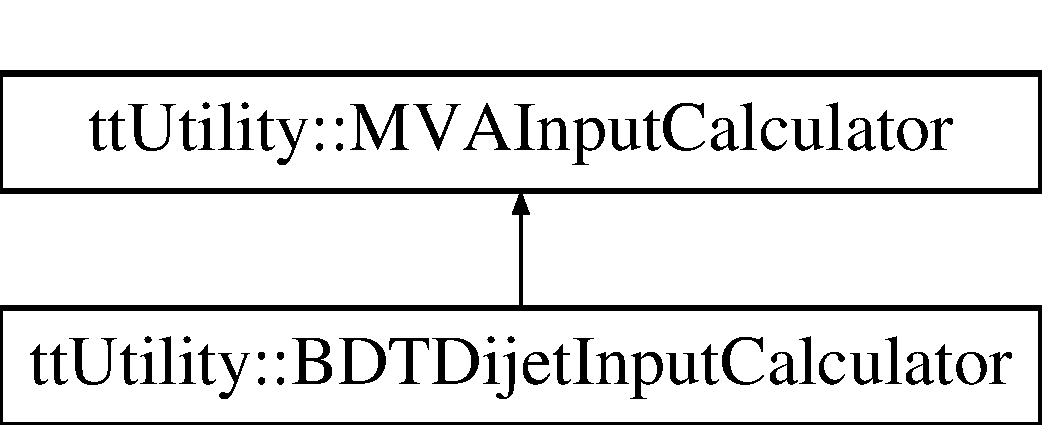
\includegraphics[height=2.000000cm]{classttUtility_1_1BDTDijetInputCalculator}
\end{center}
\end{figure}
\subsection*{Public Member Functions}
\begin{DoxyCompactItemize}
\item 
void \hyperlink{classttUtility_1_1BDTDijetInputCalculator_a8b3197ff6ced189b17e3d666ef8f24a7}{map\-Vars} (const std\-::vector$<$ std\-::string $>$ \&)
\item 
bool \hyperlink{classttUtility_1_1BDTDijetInputCalculator_aabe1eff89a230cc1a02606eaadc74fdc}{calculate\-Vars} (const \hyperlink{classTopObject}{Top\-Object} \&, int)
\item 
bool \hyperlink{classttUtility_1_1BDTDijetInputCalculator_a2832dae8ebcb1572c05379776c67d4ef}{check\-Cand} (const \hyperlink{classTopObject}{Top\-Object} \&)
\end{DoxyCompactItemize}
\subsection*{Additional Inherited Members}


\subsection{Detailed Description}
Class to calculate the input variables for the B\-D\-T based A\-K8 W selection 

\subsection{Member Function Documentation}
\hypertarget{classttUtility_1_1BDTDijetInputCalculator_aabe1eff89a230cc1a02606eaadc74fdc}{\index{tt\-Utility\-::\-B\-D\-T\-Dijet\-Input\-Calculator@{tt\-Utility\-::\-B\-D\-T\-Dijet\-Input\-Calculator}!calculate\-Vars@{calculate\-Vars}}
\index{calculate\-Vars@{calculate\-Vars}!ttUtility::BDTDijetInputCalculator@{tt\-Utility\-::\-B\-D\-T\-Dijet\-Input\-Calculator}}
\subsubsection[{calculate\-Vars}]{\setlength{\rightskip}{0pt plus 5cm}bool tt\-Utility\-::\-B\-D\-T\-Dijet\-Input\-Calculator\-::calculate\-Vars (
\begin{DoxyParamCaption}
\item[{const {\bf Top\-Object} \&}]{, }
\item[{int}]{}
\end{DoxyParamCaption}
)\hspace{0.3cm}{\ttfamily [virtual]}}}\label{classttUtility_1_1BDTDijetInputCalculator_aabe1eff89a230cc1a02606eaadc74fdc}
Calculate the requested variables and store the values directly in the input array for the M\-V\-A 
\begin{DoxyParams}{Parameters}
{\em top\-Cand} & the top candidate to calculate the input variables for \\
\hline
\end{DoxyParams}


Implements \hyperlink{classttUtility_1_1MVAInputCalculator_a86793cfa66ca816b2e1667a6b12db7d8}{tt\-Utility\-::\-M\-V\-A\-Input\-Calculator}.

\hypertarget{classttUtility_1_1BDTDijetInputCalculator_a2832dae8ebcb1572c05379776c67d4ef}{\index{tt\-Utility\-::\-B\-D\-T\-Dijet\-Input\-Calculator@{tt\-Utility\-::\-B\-D\-T\-Dijet\-Input\-Calculator}!check\-Cand@{check\-Cand}}
\index{check\-Cand@{check\-Cand}!ttUtility::BDTDijetInputCalculator@{tt\-Utility\-::\-B\-D\-T\-Dijet\-Input\-Calculator}}
\subsubsection[{check\-Cand}]{\setlength{\rightskip}{0pt plus 5cm}bool tt\-Utility\-::\-B\-D\-T\-Dijet\-Input\-Calculator\-::check\-Cand (
\begin{DoxyParamCaption}
\item[{const {\bf Top\-Object} \&}]{}
\end{DoxyParamCaption}
)\hspace{0.3cm}{\ttfamily [virtual]}}}\label{classttUtility_1_1BDTDijetInputCalculator_a2832dae8ebcb1572c05379776c67d4ef}
Check if the \hyperlink{classTopObject}{Top\-Object} passes basic selection for this category. 
\begin{DoxyParams}{Parameters}
{\em top\-Cand} & the top candidate to check \\
\hline
\end{DoxyParams}


Implements \hyperlink{classttUtility_1_1MVAInputCalculator_ae8df426d7943b921c0b9d086d1ccde30}{tt\-Utility\-::\-M\-V\-A\-Input\-Calculator}.

\hypertarget{classttUtility_1_1BDTDijetInputCalculator_a8b3197ff6ced189b17e3d666ef8f24a7}{\index{tt\-Utility\-::\-B\-D\-T\-Dijet\-Input\-Calculator@{tt\-Utility\-::\-B\-D\-T\-Dijet\-Input\-Calculator}!map\-Vars@{map\-Vars}}
\index{map\-Vars@{map\-Vars}!ttUtility::BDTDijetInputCalculator@{tt\-Utility\-::\-B\-D\-T\-Dijet\-Input\-Calculator}}
\subsubsection[{map\-Vars}]{\setlength{\rightskip}{0pt plus 5cm}void tt\-Utility\-::\-B\-D\-T\-Dijet\-Input\-Calculator\-::map\-Vars (
\begin{DoxyParamCaption}
\item[{const std\-::vector$<$ std\-::string $>$ \&}]{}
\end{DoxyParamCaption}
)\hspace{0.3cm}{\ttfamily [virtual]}}}\label{classttUtility_1_1BDTDijetInputCalculator_a8b3197ff6ced189b17e3d666ef8f24a7}
The job of map\-Vars is to populate the internal offests for all variables in the input variable list with their memory location in the data array. To be called only once. 
\begin{DoxyParams}{Parameters}
{\em vars} & list of variables used for the model \\
\hline
\end{DoxyParams}


Implements \hyperlink{classttUtility_1_1MVAInputCalculator_aca315e5c5ce1d110660eb54cd7facfd8}{tt\-Utility\-::\-M\-V\-A\-Input\-Calculator}.



The documentation for this class was generated from the following files\-:\begin{DoxyCompactItemize}
\item 
/home/travis/build/susy2015/\-Top\-Tagger/\-Top\-Tagger/include/\hyperlink{TopTaggerUtilities_8h}{Top\-Tagger\-Utilities.\-h}\item 
/home/travis/build/susy2015/\-Top\-Tagger/\-Top\-Tagger/src/Top\-Tagger\-Utilities.\-cpp\end{DoxyCompactItemize}

\hypertarget{classttUtility_1_1BDTMonojetInputCalculator}{\section{tt\-Utility\-:\-:B\-D\-T\-Monojet\-Input\-Calculator Class Reference}
\label{classttUtility_1_1BDTMonojetInputCalculator}\index{tt\-Utility\-::\-B\-D\-T\-Monojet\-Input\-Calculator@{tt\-Utility\-::\-B\-D\-T\-Monojet\-Input\-Calculator}}
}


{\ttfamily \#include $<$Top\-Tagger\-Utilities.\-h$>$}

Inheritance diagram for tt\-Utility\-:\-:B\-D\-T\-Monojet\-Input\-Calculator\-:\begin{figure}[H]
\begin{center}
\leavevmode
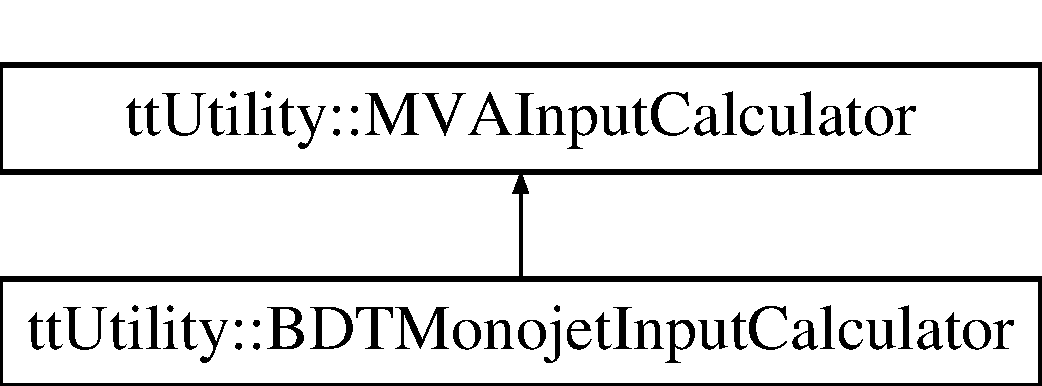
\includegraphics[height=2.000000cm]{classttUtility_1_1BDTMonojetInputCalculator}
\end{center}
\end{figure}
\subsection*{Public Member Functions}
\begin{DoxyCompactItemize}
\item 
void \hyperlink{classttUtility_1_1BDTMonojetInputCalculator_af929778a33ce64a1c5102712a2858aa0}{map\-Vars} (const std\-::vector$<$ std\-::string $>$ \&)
\item 
bool \hyperlink{classttUtility_1_1BDTMonojetInputCalculator_ade65c192d67eb363a4b4028b4f0ec7c5}{calculate\-Vars} (const \hyperlink{classTopObject}{Top\-Object} \&, int)
\item 
bool \hyperlink{classttUtility_1_1BDTMonojetInputCalculator_aabe30d40a85c15a5c4df89f39b44be88}{check\-Cand} (const \hyperlink{classTopObject}{Top\-Object} \&)
\end{DoxyCompactItemize}
\subsection*{Additional Inherited Members}


\subsection{Detailed Description}
Class to calculate the input variables for the B\-D\-T based A\-K8 top selection 

\subsection{Member Function Documentation}
\hypertarget{classttUtility_1_1BDTMonojetInputCalculator_ade65c192d67eb363a4b4028b4f0ec7c5}{\index{tt\-Utility\-::\-B\-D\-T\-Monojet\-Input\-Calculator@{tt\-Utility\-::\-B\-D\-T\-Monojet\-Input\-Calculator}!calculate\-Vars@{calculate\-Vars}}
\index{calculate\-Vars@{calculate\-Vars}!ttUtility::BDTMonojetInputCalculator@{tt\-Utility\-::\-B\-D\-T\-Monojet\-Input\-Calculator}}
\subsubsection[{calculate\-Vars}]{\setlength{\rightskip}{0pt plus 5cm}bool tt\-Utility\-::\-B\-D\-T\-Monojet\-Input\-Calculator\-::calculate\-Vars (
\begin{DoxyParamCaption}
\item[{const {\bf Top\-Object} \&}]{, }
\item[{int}]{}
\end{DoxyParamCaption}
)\hspace{0.3cm}{\ttfamily [virtual]}}}\label{classttUtility_1_1BDTMonojetInputCalculator_ade65c192d67eb363a4b4028b4f0ec7c5}
Calculate the requested variables and store the values directly in the input array for the M\-V\-A 
\begin{DoxyParams}{Parameters}
{\em top\-Cand} & the top candidate to calculate the input variables for \\
\hline
\end{DoxyParams}


Implements \hyperlink{classttUtility_1_1MVAInputCalculator_a86793cfa66ca816b2e1667a6b12db7d8}{tt\-Utility\-::\-M\-V\-A\-Input\-Calculator}.

\hypertarget{classttUtility_1_1BDTMonojetInputCalculator_aabe30d40a85c15a5c4df89f39b44be88}{\index{tt\-Utility\-::\-B\-D\-T\-Monojet\-Input\-Calculator@{tt\-Utility\-::\-B\-D\-T\-Monojet\-Input\-Calculator}!check\-Cand@{check\-Cand}}
\index{check\-Cand@{check\-Cand}!ttUtility::BDTMonojetInputCalculator@{tt\-Utility\-::\-B\-D\-T\-Monojet\-Input\-Calculator}}
\subsubsection[{check\-Cand}]{\setlength{\rightskip}{0pt plus 5cm}bool tt\-Utility\-::\-B\-D\-T\-Monojet\-Input\-Calculator\-::check\-Cand (
\begin{DoxyParamCaption}
\item[{const {\bf Top\-Object} \&}]{}
\end{DoxyParamCaption}
)\hspace{0.3cm}{\ttfamily [virtual]}}}\label{classttUtility_1_1BDTMonojetInputCalculator_aabe30d40a85c15a5c4df89f39b44be88}
Check if the \hyperlink{classTopObject}{Top\-Object} passes basic selection for this category. 
\begin{DoxyParams}{Parameters}
{\em top\-Cand} & the top candidate to check \\
\hline
\end{DoxyParams}


Implements \hyperlink{classttUtility_1_1MVAInputCalculator_ae8df426d7943b921c0b9d086d1ccde30}{tt\-Utility\-::\-M\-V\-A\-Input\-Calculator}.

\hypertarget{classttUtility_1_1BDTMonojetInputCalculator_af929778a33ce64a1c5102712a2858aa0}{\index{tt\-Utility\-::\-B\-D\-T\-Monojet\-Input\-Calculator@{tt\-Utility\-::\-B\-D\-T\-Monojet\-Input\-Calculator}!map\-Vars@{map\-Vars}}
\index{map\-Vars@{map\-Vars}!ttUtility::BDTMonojetInputCalculator@{tt\-Utility\-::\-B\-D\-T\-Monojet\-Input\-Calculator}}
\subsubsection[{map\-Vars}]{\setlength{\rightskip}{0pt plus 5cm}void tt\-Utility\-::\-B\-D\-T\-Monojet\-Input\-Calculator\-::map\-Vars (
\begin{DoxyParamCaption}
\item[{const std\-::vector$<$ std\-::string $>$ \&}]{}
\end{DoxyParamCaption}
)\hspace{0.3cm}{\ttfamily [virtual]}}}\label{classttUtility_1_1BDTMonojetInputCalculator_af929778a33ce64a1c5102712a2858aa0}
The job of map\-Vars is to populate the internal offests for all variables in the input variable list with their memory location in the data array. To be called only once. 
\begin{DoxyParams}{Parameters}
{\em vars} & list of variables used for the model \\
\hline
\end{DoxyParams}


Implements \hyperlink{classttUtility_1_1MVAInputCalculator_aca315e5c5ce1d110660eb54cd7facfd8}{tt\-Utility\-::\-M\-V\-A\-Input\-Calculator}.



The documentation for this class was generated from the following files\-:\begin{DoxyCompactItemize}
\item 
/home/travis/build/susy2015/\-Top\-Tagger/\-Top\-Tagger/include/\hyperlink{TopTaggerUtilities_8h}{Top\-Tagger\-Utilities.\-h}\item 
/home/travis/build/susy2015/\-Top\-Tagger/\-Top\-Tagger/src/Top\-Tagger\-Utilities.\-cpp\end{DoxyCompactItemize}

\hypertarget{classhcalcfg_1_1Buffer}{\section{hcalcfg\-:\-:Buffer Class Reference}
\label{classhcalcfg_1_1Buffer}\index{hcalcfg\-::\-Buffer@{hcalcfg\-::\-Buffer}}
}
Inheritance diagram for hcalcfg\-:\-:Buffer\-:\begin{figure}[H]
\begin{center}
\leavevmode
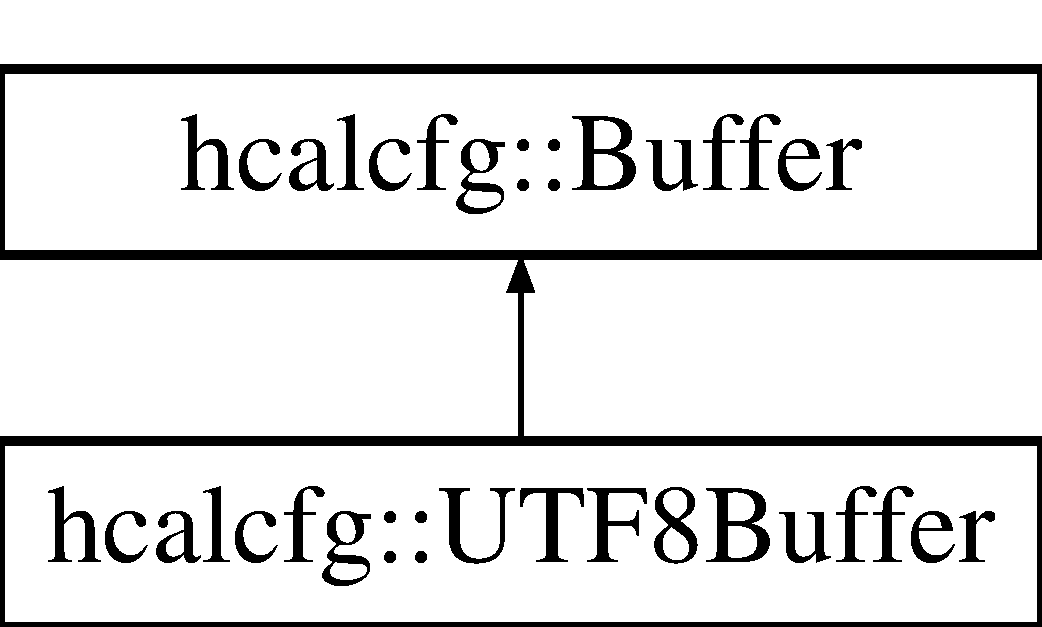
\includegraphics[height=2.000000cm]{classhcalcfg_1_1Buffer}
\end{center}
\end{figure}
\subsection*{Public Member Functions}
\begin{DoxyCompactItemize}
\item 
\hypertarget{classhcalcfg_1_1Buffer_a6735d28a4c76dee7be232d530a07b60e}{{\bfseries Buffer} (F\-I\-L\-E $\ast$s, bool is\-User\-Stream)}\label{classhcalcfg_1_1Buffer_a6735d28a4c76dee7be232d530a07b60e}

\item 
\hypertarget{classhcalcfg_1_1Buffer_a5068bfeda1634b7715c62b2f39a0e468}{{\bfseries Buffer} (const unsigned char $\ast$buf, int len)}\label{classhcalcfg_1_1Buffer_a5068bfeda1634b7715c62b2f39a0e468}

\item 
\hypertarget{classhcalcfg_1_1Buffer_a6c495bda9a7f3e1c0a7b6ce8982c576e}{{\bfseries Buffer} (\hyperlink{classhcalcfg_1_1Buffer}{Buffer} $\ast$b)}\label{classhcalcfg_1_1Buffer_a6c495bda9a7f3e1c0a7b6ce8982c576e}

\item 
\hypertarget{classhcalcfg_1_1Buffer_af5984879adeef127f92cd86a245ad3ff}{virtual void {\bfseries Close} ()}\label{classhcalcfg_1_1Buffer_af5984879adeef127f92cd86a245ad3ff}

\item 
\hypertarget{classhcalcfg_1_1Buffer_a6f4e6745827a2ea9aeae549bee15b121}{virtual int {\bfseries Read} ()}\label{classhcalcfg_1_1Buffer_a6f4e6745827a2ea9aeae549bee15b121}

\item 
\hypertarget{classhcalcfg_1_1Buffer_acd87c180ecc347a9920583cd130e87e4}{virtual int {\bfseries Peek} ()}\label{classhcalcfg_1_1Buffer_acd87c180ecc347a9920583cd130e87e4}

\item 
\hypertarget{classhcalcfg_1_1Buffer_aeaab9876bd4f9adf7e1b651574bc1eed}{virtual wchar\-\_\-t $\ast$ {\bfseries Get\-String} (int beg, int end)}\label{classhcalcfg_1_1Buffer_aeaab9876bd4f9adf7e1b651574bc1eed}

\item 
\hypertarget{classhcalcfg_1_1Buffer_a299500fb0e0f987d0d9a0531a02d0462}{virtual int {\bfseries Get\-Pos} ()}\label{classhcalcfg_1_1Buffer_a299500fb0e0f987d0d9a0531a02d0462}

\item 
\hypertarget{classhcalcfg_1_1Buffer_a2efe7843a251fc016a4ca9d47c8dc4f4}{virtual void {\bfseries Set\-Pos} (int value)}\label{classhcalcfg_1_1Buffer_a2efe7843a251fc016a4ca9d47c8dc4f4}

\end{DoxyCompactItemize}
\subsection*{Static Public Attributes}
\begin{DoxyCompactItemize}
\item 
\hypertarget{classhcalcfg_1_1Buffer_a2797e70d809eb3b5650edb732d6584d0}{static const int {\bfseries Eo\-F} = C\-O\-C\-O\-\_\-\-W\-C\-H\-A\-R\-\_\-\-M\-A\-X + 1}\label{classhcalcfg_1_1Buffer_a2797e70d809eb3b5650edb732d6584d0}

\end{DoxyCompactItemize}


The documentation for this class was generated from the following files\-:\begin{DoxyCompactItemize}
\item 
/home/travis/build/susy2015/\-Top\-Tagger/\-Cfg\-Parser/include/Scanner.\-h\item 
/home/travis/build/susy2015/\-Top\-Tagger/\-Cfg\-Parser/src/Scanner.\-cpp\end{DoxyCompactItemize}

\hypertarget{classCfgBuilder}{\section{Cfg\-Builder Class Reference}
\label{classCfgBuilder}\index{Cfg\-Builder@{Cfg\-Builder}}
}
\subsection*{Public Member Functions}
\begin{DoxyCompactItemize}
\item 
\hypertarget{classCfgBuilder_a5af2d2e469dbe4c403727f27bcad6ba3}{void {\bfseries setup} ()}\label{classCfgBuilder_a5af2d2e469dbe4c403727f27bcad6ba3}

\item 
\hypertarget{classCfgBuilder_afd5db277b02899116fb115e23a2ffd50}{std\-::unique\-\_\-ptr$<$ \hyperlink{classcfg_1_1CfgDocument}{cfg\-::\-Cfg\-Document} $>$ {\bfseries take\-Doc} ()}\label{classCfgBuilder_afd5db277b02899116fb115e23a2ffd50}

\item 
\hypertarget{classCfgBuilder_ac105e810c5cf5c7f8a053614f3f2987a}{\hyperlink{classcfg_1_1SimpleTerm}{cfg\-::\-Simple\-Term} $\ast$ {\bfseries simple\-Term} (const std\-::string \&ident, const std\-::string \&op)}\label{classCfgBuilder_ac105e810c5cf5c7f8a053614f3f2987a}

\item 
\hypertarget{classCfgBuilder_acb5a4d224b4a0dbc23d8bdde4fbf3312}{\hyperlink{classcfg_1_1SimpleTerm}{cfg\-::\-Simple\-Term} $\ast$ {\bfseries list\-Term} (const std\-::string \&ident, const std\-::string \&op)}\label{classCfgBuilder_acb5a4d224b4a0dbc23d8bdde4fbf3312}

\item 
\hypertarget{classCfgBuilder_aa8c4e0c4b955a6ada763bafce754d3a2}{void {\bfseries assign} ()}\label{classCfgBuilder_aa8c4e0c4b955a6ada763bafce754d3a2}

\item 
\hypertarget{classCfgBuilder_af74e188fb692e1895b36ec09bd9a1afe}{void {\bfseries i\-Literal} (wchar\-\_\-t $\ast$data)}\label{classCfgBuilder_af74e188fb692e1895b36ec09bd9a1afe}

\item 
\hypertarget{classCfgBuilder_a59e3ae228a32d5d04f929f032c9cdd42}{void {\bfseries f\-Literal} (wchar\-\_\-t $\ast$data)}\label{classCfgBuilder_a59e3ae228a32d5d04f929f032c9cdd42}

\item 
\hypertarget{classCfgBuilder_a1e908f4837c367f05385dd63e38d3e4c}{void {\bfseries b\-Literal} (bool b)}\label{classCfgBuilder_a1e908f4837c367f05385dd63e38d3e4c}

\item 
\hypertarget{classCfgBuilder_ab213a7e0ed2e294ced2f08e1f79b5d37}{void {\bfseries s\-Literal} (const wchar\-\_\-t $\ast$data)}\label{classCfgBuilder_ab213a7e0ed2e294ced2f08e1f79b5d37}

\item 
\hypertarget{classCfgBuilder_a6afd2f47b9a7e107e236e9015d9be3a7}{\hyperlink{classcfg_1_1Condition}{cfg\-::\-Condition} $\ast$ {\bfseries new\-Condition} ()}\label{classCfgBuilder_a6afd2f47b9a7e107e236e9015d9be3a7}

\item 
\hypertarget{classCfgBuilder_aa995c209a3708a6776de7b568d37fcbf}{void {\bfseries pop\-Condition} ()}\label{classCfgBuilder_aa995c209a3708a6776de7b568d37fcbf}

\item 
\hypertarget{classCfgBuilder_a50ddecd4930af4282b10f31d3e17578d}{void {\bfseries set\-Namespace} (const std\-::string \&s)}\label{classCfgBuilder_a50ddecd4930af4282b10f31d3e17578d}

\end{DoxyCompactItemize}
\subsection*{Static Public Member Functions}
\begin{DoxyCompactItemize}
\item 
\hypertarget{classCfgBuilder_a7bd5f3def6b00f071877b2b81bb4c25a}{static std\-::string {\bfseries to\-String} (const wchar\-\_\-t $\ast$d)}\label{classCfgBuilder_a7bd5f3def6b00f071877b2b81bb4c25a}

\item 
\hypertarget{classCfgBuilder_aa620acd787a50158dd4a7e879a7fa8e3}{static int {\bfseries to\-Int} (const wchar\-\_\-t $\ast$d)}\label{classCfgBuilder_aa620acd787a50158dd4a7e879a7fa8e3}

\end{DoxyCompactItemize}
\subsection*{Public Attributes}
\begin{DoxyCompactItemize}
\item 
\hypertarget{classCfgBuilder_aa4534dcb2ec75d02d178b24c9cf30b8d}{std\-::vector$<$ \hyperlink{classcfg_1_1Literal}{cfg\-::\-Literal} $>$ {\bfseries literal\-Stack}}\label{classCfgBuilder_aa4534dcb2ec75d02d178b24c9cf30b8d}

\item 
\hypertarget{classCfgBuilder_ac326d1e9426b9d15afae30a4f6c1313f}{\hyperlink{classcfg_1_1ConditionChain}{cfg\-::\-Condition\-Chain} {\bfseries active\-Chain}}\label{classCfgBuilder_ac326d1e9426b9d15afae30a4f6c1313f}

\item 
\hypertarget{classCfgBuilder_ab376ec6aad26f59bf931c3e6f5c2b20f}{\hyperlink{classcfg_1_1Term}{cfg\-::\-Term} $\ast$ {\bfseries last\-Term}}\label{classCfgBuilder_ab376ec6aad26f59bf931c3e6f5c2b20f}

\item 
\hypertarget{classCfgBuilder_a5dcb7004ac3ff2ee353c828339343569}{std\-::string {\bfseries the\-Namespace}}\label{classCfgBuilder_a5dcb7004ac3ff2ee353c828339343569}

\item 
\hypertarget{classCfgBuilder_a103ff056b767b8456ae538f26370ba78}{std\-::string {\bfseries the\-Item\-Name}}\label{classCfgBuilder_a103ff056b767b8456ae538f26370ba78}

\item 
\hypertarget{classCfgBuilder_a2f69af14667df0c44f4052f653bd6067}{int {\bfseries the\-Item\-Index}}\label{classCfgBuilder_a2f69af14667df0c44f4052f653bd6067}

\item 
\hypertarget{classCfgBuilder_acdcea7422a4c083bd0dc6dfb27ea10b1}{std\-::unique\-\_\-ptr$<$ \hyperlink{classcfg_1_1CfgDocument}{cfg\-::\-Cfg\-Document} $>$ {\bfseries the\-Doc}}\label{classCfgBuilder_acdcea7422a4c083bd0dc6dfb27ea10b1}

\end{DoxyCompactItemize}


The documentation for this class was generated from the following file\-:\begin{DoxyCompactItemize}
\item 
/home/travis/build/susy2015/\-Top\-Tagger/\-Cfg\-Parser/include/Defs.\-h\end{DoxyCompactItemize}

\hypertarget{classcfg_1_1CfgDocument}{\section{cfg\-:\-:Cfg\-Document Class Reference}
\label{classcfg_1_1CfgDocument}\index{cfg\-::\-Cfg\-Document@{cfg\-::\-Cfg\-Document}}
}
\subsection*{Public Types}
\begin{DoxyCompactItemize}
\item 
\hypertarget{classcfg_1_1CfgDocument_ab40d2ad0600280de539ad7022ced6a95}{typedef std\-::map$<$ std\-::string, \\*
std\-::unique\-\_\-ptr$<$ \hyperlink{classcfg_1_1Parameter}{Parameter} $>$\\*
 $>$\-::const\-\_\-iterator {\bfseries param\-\_\-itr}}\label{classcfg_1_1CfgDocument_ab40d2ad0600280de539ad7022ced6a95}

\end{DoxyCompactItemize}
\subsection*{Public Member Functions}
\begin{DoxyCompactItemize}
\item 
\hypertarget{classcfg_1_1CfgDocument_a7e9717619972b99699367c1d55978b23}{void {\bfseries use\-Record} (\hyperlink{classcfg_1_1Record}{Record} $\ast$)}\label{classcfg_1_1CfgDocument_a7e9717619972b99699367c1d55978b23}

\item 
\hypertarget{classcfg_1_1CfgDocument_a13259bc4813ea81c8a19d23ac7a66e0e}{\hyperlink{classcfg_1_1Condition}{Condition} $\ast$ {\bfseries add\-Condition} ()}\label{classcfg_1_1CfgDocument_a13259bc4813ea81c8a19d23ac7a66e0e}

\item 
\hypertarget{classcfg_1_1CfgDocument_a563af2fe3335a03c7ce2b49aeb01b251}{void {\bfseries assign\-Parameter} (const std\-::string \&ns, const std\-::string \&name, const \hyperlink{classcfg_1_1ConditionChain}{Condition\-Chain} \&cc, const \hyperlink{classcfg_1_1Literal}{Literal} \&l)}\label{classcfg_1_1CfgDocument_a563af2fe3335a03c7ce2b49aeb01b251}

\item 
\hypertarget{classcfg_1_1CfgDocument_a6b7c7570b0f29381e06fbcd4f14bf5a0}{int {\bfseries get} (const std\-::string \&name, const \hyperlink{classcfg_1_1Context}{Context} \&cxt, int defl) const }\label{classcfg_1_1CfgDocument_a6b7c7570b0f29381e06fbcd4f14bf5a0}

\item 
\hypertarget{classcfg_1_1CfgDocument_adcfac4c55418d640d2a92584f9cc7f84}{double {\bfseries get} (const std\-::string \&name, const \hyperlink{classcfg_1_1Context}{Context} \&cxt, double defl) const }\label{classcfg_1_1CfgDocument_adcfac4c55418d640d2a92584f9cc7f84}

\item 
\hypertarget{classcfg_1_1CfgDocument_a2f205dc62685981c29bd01d8b110ca64}{bool {\bfseries get} (const std\-::string \&name, const \hyperlink{classcfg_1_1Context}{Context} \&cxt, bool defl) const }\label{classcfg_1_1CfgDocument_a2f205dc62685981c29bd01d8b110ca64}

\item 
\hypertarget{classcfg_1_1CfgDocument_a126dda4f1bb8732e531e4371ef15589e}{std\-::string {\bfseries get} (const std\-::string \&name, const \hyperlink{classcfg_1_1Context}{Context} \&cxt, const char $\ast$defl) const }\label{classcfg_1_1CfgDocument_a126dda4f1bb8732e531e4371ef15589e}

\item 
\hypertarget{classcfg_1_1CfgDocument_a88fa62b435821b5ac383b1590ec6b7c5}{std\-::string {\bfseries get} (const std\-::string \&name, const \hyperlink{classcfg_1_1Context}{Context} \&cxt, const std\-::string \&defl) const }\label{classcfg_1_1CfgDocument_a88fa62b435821b5ac383b1590ec6b7c5}

\item 
\hypertarget{classcfg_1_1CfgDocument_abfbca1fb73590965a5d13cfaea5a673a}{int {\bfseries get} (const std\-::string \&name, int index, const \hyperlink{classcfg_1_1Context}{Context} \&cxt, int defl) const }\label{classcfg_1_1CfgDocument_abfbca1fb73590965a5d13cfaea5a673a}

\item 
\hypertarget{classcfg_1_1CfgDocument_afdf2735d5bf9f4272bf960042310e9e6}{double {\bfseries get} (const std\-::string \&name, int index, const \hyperlink{classcfg_1_1Context}{Context} \&cxt, double defl) const }\label{classcfg_1_1CfgDocument_afdf2735d5bf9f4272bf960042310e9e6}

\item 
\hypertarget{classcfg_1_1CfgDocument_a991d7e1aa02b091cd000f0f00a8ab122}{bool {\bfseries get} (const std\-::string \&name, int index, const \hyperlink{classcfg_1_1Context}{Context} \&cxt, bool defl) const }\label{classcfg_1_1CfgDocument_a991d7e1aa02b091cd000f0f00a8ab122}

\item 
\hypertarget{classcfg_1_1CfgDocument_a9742250a76addffa269e2035362aebe1}{std\-::string {\bfseries get} (const std\-::string \&name, int index, const \hyperlink{classcfg_1_1Context}{Context} \&cxt, const char $\ast$defl) const }\label{classcfg_1_1CfgDocument_a9742250a76addffa269e2035362aebe1}

\item 
\hypertarget{classcfg_1_1CfgDocument_a923b2862c1126f0193a7e8a9e51302dd}{std\-::string {\bfseries get} (const std\-::string \&name, int index, const \hyperlink{classcfg_1_1Context}{Context} \&cxt, const std\-::string \&defl) const }\label{classcfg_1_1CfgDocument_a923b2862c1126f0193a7e8a9e51302dd}

\item 
\hypertarget{classcfg_1_1CfgDocument_ac2f9bd72ddc1e1ddec9d7cec23bc20af}{param\-\_\-itr {\bfseries param\-\_\-begin} () const }\label{classcfg_1_1CfgDocument_ac2f9bd72ddc1e1ddec9d7cec23bc20af}

\item 
\hypertarget{classcfg_1_1CfgDocument_acdc088167b35b8b9a061dfa39e67a829}{param\-\_\-itr {\bfseries param\-\_\-end} () const }\label{classcfg_1_1CfgDocument_acdc088167b35b8b9a061dfa39e67a829}

\item 
\hypertarget{classcfg_1_1CfgDocument_a79a2e32dd17ee0a44b3edb6c4b93ed4d}{void {\bfseries post\-Value\-Used} (const std\-::string \&name, const \hyperlink{classcfg_1_1Context}{Context} \&cxt, int value)}\label{classcfg_1_1CfgDocument_a79a2e32dd17ee0a44b3edb6c4b93ed4d}

\item 
\hypertarget{classcfg_1_1CfgDocument_ad49d863f75f92db5d3f0d382b4c56380}{void {\bfseries post\-Value\-Used} (const std\-::string \&name, const \hyperlink{classcfg_1_1Context}{Context} \&cxt, const char $\ast$value)}\label{classcfg_1_1CfgDocument_ad49d863f75f92db5d3f0d382b4c56380}

\item 
\hypertarget{classcfg_1_1CfgDocument_a6339d992b1356deb95bd6493ed76f279}{void {\bfseries post\-Value\-Used} (const std\-::string \&name, const \hyperlink{classcfg_1_1Context}{Context} \&cxt, const std\-::string \&value)}\label{classcfg_1_1CfgDocument_a6339d992b1356deb95bd6493ed76f279}

\item 
\hypertarget{classcfg_1_1CfgDocument_ae53be6f4f805749868bb734f1c8c700c}{void {\bfseries post\-Value\-Used} (const std\-::string \&name, const \hyperlink{classcfg_1_1Context}{Context} \&cxt, bool value)}\label{classcfg_1_1CfgDocument_ae53be6f4f805749868bb734f1c8c700c}

\end{DoxyCompactItemize}
\subsection*{Static Public Member Functions}
\begin{DoxyCompactItemize}
\item 
\hypertarget{classcfg_1_1CfgDocument_a5124097991f411053eb8dab6b9057dbe}{static std\-::unique\-\_\-ptr\\*
$<$ \hyperlink{classcfg_1_1CfgDocument}{Cfg\-Document} $>$ {\bfseries parse\-Document} (const std\-::string \&text)}\label{classcfg_1_1CfgDocument_a5124097991f411053eb8dab6b9057dbe}

\end{DoxyCompactItemize}


The documentation for this class was generated from the following files\-:\begin{DoxyCompactItemize}
\item 
/home/travis/build/susy2015/\-Top\-Tagger/\-Cfg\-Parser/include/Cfg\-Document.\-hh\item 
/home/travis/build/susy2015/\-Top\-Tagger/\-Cfg\-Parser/src/Cfg\-Document.\-cc\end{DoxyCompactItemize}

\hypertarget{classcfg_1_1Condition}{\section{cfg\-:\-:Condition Class Reference}
\label{classcfg_1_1Condition}\index{cfg\-::\-Condition@{cfg\-::\-Condition}}
}
\subsection*{Public Member Functions}
\begin{DoxyCompactItemize}
\item 
\hypertarget{classcfg_1_1Condition_a9f6ab9de4b9a9b159fcf1f096d71e929}{void {\bfseries set} (\hyperlink{classcfg_1_1TermAnd}{Term\-And} $\ast$ta)}\label{classcfg_1_1Condition_a9f6ab9de4b9a9b159fcf1f096d71e929}

\item 
\hypertarget{classcfg_1_1Condition_acf5fa4f635143031a3a9a013ef000d8b}{bool {\bfseries test} (const \hyperlink{classcfg_1_1Context}{Context} \&cxt) const }\label{classcfg_1_1Condition_acf5fa4f635143031a3a9a013ef000d8b}

\item 
\hypertarget{classcfg_1_1Condition_a13d6af566359dcc425dd64970dfc8cf4}{void {\bfseries and\-Term} (\hyperlink{classcfg_1_1Term}{Term} $\ast$t)}\label{classcfg_1_1Condition_a13d6af566359dcc425dd64970dfc8cf4}

\item 
\hypertarget{classcfg_1_1Condition_ab6e1f28e69efd9e7d82698b486fffb7f}{std\-::ostream \& {\bfseries put} (std\-::ostream \&o) const }\label{classcfg_1_1Condition_ab6e1f28e69efd9e7d82698b486fffb7f}

\item 
\hypertarget{classcfg_1_1Condition_a6982764b31034fe97d41b38429786702}{std\-::set$<$ std\-::string $>$ {\bfseries queried\-Items} () const }\label{classcfg_1_1Condition_a6982764b31034fe97d41b38429786702}

\end{DoxyCompactItemize}


The documentation for this class was generated from the following files\-:\begin{DoxyCompactItemize}
\item 
/home/travis/build/susy2015/\-Top\-Tagger/\-Cfg\-Parser/include/Condition.\-hh\item 
/home/travis/build/susy2015/\-Top\-Tagger/\-Cfg\-Parser/src/Condition.\-cc\end{DoxyCompactItemize}

\hypertarget{classcfg_1_1ConditionChain}{\section{cfg\-:\-:Condition\-Chain Class Reference}
\label{classcfg_1_1ConditionChain}\index{cfg\-::\-Condition\-Chain@{cfg\-::\-Condition\-Chain}}
}
\subsection*{Public Member Functions}
\begin{DoxyCompactItemize}
\item 
\hypertarget{classcfg_1_1ConditionChain_a96b7f3d5277cff3fd72bb842edbe5528}{void {\bfseries push} (const \hyperlink{classcfg_1_1Condition}{Condition} $\ast$c)}\label{classcfg_1_1ConditionChain_a96b7f3d5277cff3fd72bb842edbe5528}

\item 
\hypertarget{classcfg_1_1ConditionChain_a22fff931b71405e4e83af359c0068c1f}{void {\bfseries pop} ()}\label{classcfg_1_1ConditionChain_a22fff931b71405e4e83af359c0068c1f}

\item 
\hypertarget{classcfg_1_1ConditionChain_adf1c15e54087ff4a0421e32d63cc377d}{bool {\bfseries test} (const \hyperlink{classcfg_1_1Context}{Context} \&cxt) const }\label{classcfg_1_1ConditionChain_adf1c15e54087ff4a0421e32d63cc377d}

\item 
\hypertarget{classcfg_1_1ConditionChain_a3c44052b97a29ad20765b350a54e8cb9}{std\-::ostream \& {\bfseries put} (std\-::ostream \&o) const }\label{classcfg_1_1ConditionChain_a3c44052b97a29ad20765b350a54e8cb9}

\item 
\hypertarget{classcfg_1_1ConditionChain_a3265eb068000bb12d8f0f23753d51b85}{std\-::set$<$ std\-::string $>$ {\bfseries queried\-Items} () const }\label{classcfg_1_1ConditionChain_a3265eb068000bb12d8f0f23753d51b85}

\end{DoxyCompactItemize}


The documentation for this class was generated from the following files\-:\begin{DoxyCompactItemize}
\item 
/home/travis/build/susy2015/\-Top\-Tagger/\-Cfg\-Parser/include/Condition.\-hh\item 
/home/travis/build/susy2015/\-Top\-Tagger/\-Cfg\-Parser/src/Condition.\-cc\end{DoxyCompactItemize}

\hypertarget{classttUtility_1_1ConstAK4Inputs}{\section{tt\-Utility\-:\-:Const\-A\-K4\-Inputs$<$ F\-L\-O\-A\-T\-T\-Y\-P\-E $>$ Class Template Reference}
\label{classttUtility_1_1ConstAK4Inputs}\index{tt\-Utility\-::\-Const\-A\-K4\-Inputs$<$ F\-L\-O\-A\-T\-T\-Y\-P\-E $>$@{tt\-Utility\-::\-Const\-A\-K4\-Inputs$<$ F\-L\-O\-A\-T\-T\-Y\-P\-E $>$}}
}


{\ttfamily \#include $<$Top\-Tagger\-Utilities.\-h$>$}

Inheritance diagram for tt\-Utility\-:\-:Const\-A\-K4\-Inputs$<$ F\-L\-O\-A\-T\-T\-Y\-P\-E $>$\-:\begin{figure}[H]
\begin{center}
\leavevmode
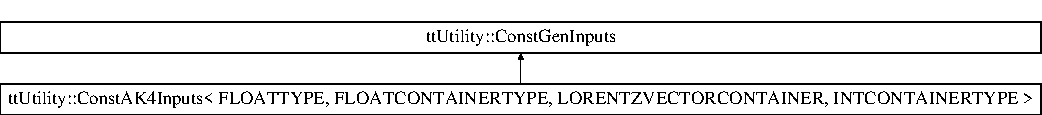
\includegraphics[height=2.000000cm]{classttUtility_1_1ConstAK4Inputs}
\end{center}
\end{figure}
\subsection*{Public Member Functions}
\begin{DoxyCompactItemize}
\item 
\hyperlink{classttUtility_1_1ConstAK4Inputs_a1c7cba3adee5f735134c23d20f30a397}{Const\-A\-K4\-Inputs} (const std\-::vector$<$ T\-Lorentz\-Vector $>$ \&jets\-L\-Vec, const std\-::vector$<$ F\-L\-O\-A\-T\-T\-Y\-P\-E $>$ \&btag\-Factors, const std\-::vector$<$ F\-L\-O\-A\-T\-T\-Y\-P\-E $>$ \&qg\-Likelihood)
\item 
\hyperlink{classttUtility_1_1ConstAK4Inputs_aeb8c14355009a3e7df17ae8db014ccc7}{Const\-A\-K4\-Inputs} (const std\-::vector$<$ T\-Lorentz\-Vector $>$ \&jets\-L\-Vec, const std\-::vector$<$ F\-L\-O\-A\-T\-T\-Y\-P\-E $>$ \&btag\-Factors)
\item 
\hyperlink{classttUtility_1_1ConstAK4Inputs_ac9906d074f5a43a6b609385ebb939204}{Const\-A\-K4\-Inputs} (const std\-::vector$<$ T\-Lorentz\-Vector $>$ \&jets\-L\-Vec, const std\-::vector$<$ F\-L\-O\-A\-T\-T\-Y\-P\-E $>$ \&btag\-Factors, const std\-::vector$<$ F\-L\-O\-A\-T\-T\-Y\-P\-E $>$ \&qg\-Likelihood, const std\-::vector$<$ T\-Lorentz\-Vector $>$ \&had\-Gen\-Tops, const std\-::vector$<$ std\-::vector$<$ const T\-Lorentz\-Vector $\ast$ $>$$>$ \&had\-Gen\-Top\-Daughters)
\item 
void \hyperlink{classttUtility_1_1ConstAK4Inputs_a4ed506e88c7e854713f52bf5f7f1652d}{add\-Q\-G\-L\-Vectors} (const std\-::vector$<$ int $>$ \&qg\-Mult, const std\-::vector$<$ F\-L\-O\-A\-T\-T\-Y\-P\-E $>$ \&qg\-Pt\-D, const std\-::vector$<$ F\-L\-O\-A\-T\-T\-Y\-P\-E $>$ \&qg\-Axis1, const std\-::vector$<$ F\-L\-O\-A\-T\-T\-Y\-P\-E $>$ \&qg\-Axis2)
\item 
void \hyperlink{classttUtility_1_1ConstAK4Inputs_aa7fc3fed9a160ab26cd77fd7c8b09565}{add\-Supplamental\-Vector} (const std\-::string \&name, const std\-::vector$<$ F\-L\-O\-A\-T\-T\-Y\-P\-E $>$ \&vector)
\item 
void \hyperlink{classttUtility_1_1ConstAK4Inputs_ab7827ad7b5906177068c107c4c8bb4d7}{package\-Constituents} (std\-::vector$<$ \hyperlink{classConstituent}{Constituent} $>$ \&constituents)
\end{DoxyCompactItemize}
\subsection*{Additional Inherited Members}


\subsection{Detailed Description}
\subsubsection*{template$<$typename F\-L\-O\-A\-T\-T\-Y\-P\-E$>$class tt\-Utility\-::\-Const\-A\-K4\-Inputs$<$ F\-L\-O\-A\-T\-T\-Y\-P\-E $>$}

Class to gather the information necessary to construct the A\-K4 jet constituents 

\subsection{Constructor \& Destructor Documentation}
\hypertarget{classttUtility_1_1ConstAK4Inputs_a1c7cba3adee5f735134c23d20f30a397}{\index{tt\-Utility\-::\-Const\-A\-K4\-Inputs@{tt\-Utility\-::\-Const\-A\-K4\-Inputs}!Const\-A\-K4\-Inputs@{Const\-A\-K4\-Inputs}}
\index{Const\-A\-K4\-Inputs@{Const\-A\-K4\-Inputs}!ttUtility::ConstAK4Inputs@{tt\-Utility\-::\-Const\-A\-K4\-Inputs}}
\subsubsection[{Const\-A\-K4\-Inputs}]{\setlength{\rightskip}{0pt plus 5cm}template$<$typename F\-L\-O\-A\-T\-T\-Y\-P\-E $>$ {\bf tt\-Utility\-::\-Const\-A\-K4\-Inputs}$<$ F\-L\-O\-A\-T\-T\-Y\-P\-E $>$\-::{\bf Const\-A\-K4\-Inputs} (
\begin{DoxyParamCaption}
\item[{const std\-::vector$<$ T\-Lorentz\-Vector $>$ \&}]{jets\-L\-Vec, }
\item[{const std\-::vector$<$ F\-L\-O\-A\-T\-T\-Y\-P\-E $>$ \&}]{btag\-Factors, }
\item[{const std\-::vector$<$ F\-L\-O\-A\-T\-T\-Y\-P\-E $>$ \&}]{qg\-Likelihood}
\end{DoxyParamCaption}
)\hspace{0.3cm}{\ttfamily [inline]}}}\label{classttUtility_1_1ConstAK4Inputs_a1c7cba3adee5f735134c23d20f30a397}
Basic constructor with Q\-G\-L 
\begin{DoxyParams}{Parameters}
{\em jets\-L\-Vec} & Jet T\-Lorentz\-Vectors for each jet \\
\hline
{\em btag\-Factors} & B-\/tag discriminators for each jet \\
\hline
{\em qg\-Likelihood} & Quark-\/gluon likelihoods for each jet \\
\hline
\end{DoxyParams}
\hypertarget{classttUtility_1_1ConstAK4Inputs_aeb8c14355009a3e7df17ae8db014ccc7}{\index{tt\-Utility\-::\-Const\-A\-K4\-Inputs@{tt\-Utility\-::\-Const\-A\-K4\-Inputs}!Const\-A\-K4\-Inputs@{Const\-A\-K4\-Inputs}}
\index{Const\-A\-K4\-Inputs@{Const\-A\-K4\-Inputs}!ttUtility::ConstAK4Inputs@{tt\-Utility\-::\-Const\-A\-K4\-Inputs}}
\subsubsection[{Const\-A\-K4\-Inputs}]{\setlength{\rightskip}{0pt plus 5cm}template$<$typename F\-L\-O\-A\-T\-T\-Y\-P\-E $>$ {\bf tt\-Utility\-::\-Const\-A\-K4\-Inputs}$<$ F\-L\-O\-A\-T\-T\-Y\-P\-E $>$\-::{\bf Const\-A\-K4\-Inputs} (
\begin{DoxyParamCaption}
\item[{const std\-::vector$<$ T\-Lorentz\-Vector $>$ \&}]{jets\-L\-Vec, }
\item[{const std\-::vector$<$ F\-L\-O\-A\-T\-T\-Y\-P\-E $>$ \&}]{btag\-Factors}
\end{DoxyParamCaption}
)\hspace{0.3cm}{\ttfamily [inline]}}}\label{classttUtility_1_1ConstAK4Inputs_aeb8c14355009a3e7df17ae8db014ccc7}
Basic constructor 
\begin{DoxyParams}{Parameters}
{\em jets\-L\-Vec} & Jet T\-Lorentz\-Vectors for each jet \\
\hline
{\em btag\-Factors} & B-\/tag discriminators for each jet \\
\hline
\end{DoxyParams}
\hypertarget{classttUtility_1_1ConstAK4Inputs_ac9906d074f5a43a6b609385ebb939204}{\index{tt\-Utility\-::\-Const\-A\-K4\-Inputs@{tt\-Utility\-::\-Const\-A\-K4\-Inputs}!Const\-A\-K4\-Inputs@{Const\-A\-K4\-Inputs}}
\index{Const\-A\-K4\-Inputs@{Const\-A\-K4\-Inputs}!ttUtility::ConstAK4Inputs@{tt\-Utility\-::\-Const\-A\-K4\-Inputs}}
\subsubsection[{Const\-A\-K4\-Inputs}]{\setlength{\rightskip}{0pt plus 5cm}template$<$typename F\-L\-O\-A\-T\-T\-Y\-P\-E $>$ {\bf tt\-Utility\-::\-Const\-A\-K4\-Inputs}$<$ F\-L\-O\-A\-T\-T\-Y\-P\-E $>$\-::{\bf Const\-A\-K4\-Inputs} (
\begin{DoxyParamCaption}
\item[{const std\-::vector$<$ T\-Lorentz\-Vector $>$ \&}]{jets\-L\-Vec, }
\item[{const std\-::vector$<$ F\-L\-O\-A\-T\-T\-Y\-P\-E $>$ \&}]{btag\-Factors, }
\item[{const std\-::vector$<$ F\-L\-O\-A\-T\-T\-Y\-P\-E $>$ \&}]{qg\-Likelihood, }
\item[{const std\-::vector$<$ T\-Lorentz\-Vector $>$ \&}]{had\-Gen\-Tops, }
\item[{const std\-::vector$<$ std\-::vector$<$ const T\-Lorentz\-Vector $\ast$ $>$$>$ \&}]{had\-Gen\-Top\-Daughters}
\end{DoxyParamCaption}
)\hspace{0.3cm}{\ttfamily [inline]}}}\label{classttUtility_1_1ConstAK4Inputs_ac9906d074f5a43a6b609385ebb939204}
Constructor with gen informaion 
\begin{DoxyParams}{Parameters}
{\em jets\-L\-Vec} & Jet T\-Lorentz\-Vectors for each jet \\
\hline
{\em btag\-Factors} & B-\/tag discriminators for each jet \\
\hline
{\em qg\-Likelihood} & Quark-\/gluon likelihoods for each jet \\
\hline
{\em had\-Gen\-Tops} & Vector of hadronicly decaying gen top T\-Lorentz\-Vectors \\
\hline
{\em had\-Gen\-Top\-Daughters} & Vector of direct decay daughters of the top quarks \\
\hline
\end{DoxyParams}


\subsection{Member Function Documentation}
\hypertarget{classttUtility_1_1ConstAK4Inputs_a4ed506e88c7e854713f52bf5f7f1652d}{\index{tt\-Utility\-::\-Const\-A\-K4\-Inputs@{tt\-Utility\-::\-Const\-A\-K4\-Inputs}!add\-Q\-G\-L\-Vectors@{add\-Q\-G\-L\-Vectors}}
\index{add\-Q\-G\-L\-Vectors@{add\-Q\-G\-L\-Vectors}!ttUtility::ConstAK4Inputs@{tt\-Utility\-::\-Const\-A\-K4\-Inputs}}
\subsubsection[{add\-Q\-G\-L\-Vectors}]{\setlength{\rightskip}{0pt plus 5cm}template$<$typename F\-L\-O\-A\-T\-T\-Y\-P\-E $>$ void {\bf tt\-Utility\-::\-Const\-A\-K4\-Inputs}$<$ F\-L\-O\-A\-T\-T\-Y\-P\-E $>$\-::add\-Q\-G\-L\-Vectors (
\begin{DoxyParamCaption}
\item[{const std\-::vector$<$ int $>$ \&}]{qg\-Mult, }
\item[{const std\-::vector$<$ F\-L\-O\-A\-T\-T\-Y\-P\-E $>$ \&}]{qg\-Pt\-D, }
\item[{const std\-::vector$<$ F\-L\-O\-A\-T\-T\-Y\-P\-E $>$ \&}]{qg\-Axis1, }
\item[{const std\-::vector$<$ F\-L\-O\-A\-T\-T\-Y\-P\-E $>$ \&}]{qg\-Axis2}
\end{DoxyParamCaption}
)\hspace{0.3cm}{\ttfamily [inline]}}}\label{classttUtility_1_1ConstAK4Inputs_a4ed506e88c7e854713f52bf5f7f1652d}
Adds jet shape inputs from the quark-\/gluon likelihood calculator \hypertarget{classttUtility_1_1ConstAK4Inputs_aa7fc3fed9a160ab26cd77fd7c8b09565}{\index{tt\-Utility\-::\-Const\-A\-K4\-Inputs@{tt\-Utility\-::\-Const\-A\-K4\-Inputs}!add\-Supplamental\-Vector@{add\-Supplamental\-Vector}}
\index{add\-Supplamental\-Vector@{add\-Supplamental\-Vector}!ttUtility::ConstAK4Inputs@{tt\-Utility\-::\-Const\-A\-K4\-Inputs}}
\subsubsection[{add\-Supplamental\-Vector}]{\setlength{\rightskip}{0pt plus 5cm}template$<$typename F\-L\-O\-A\-T\-T\-Y\-P\-E $>$ void {\bf tt\-Utility\-::\-Const\-A\-K4\-Inputs}$<$ F\-L\-O\-A\-T\-T\-Y\-P\-E $>$\-::add\-Supplamental\-Vector (
\begin{DoxyParamCaption}
\item[{const std\-::string \&}]{name, }
\item[{const std\-::vector$<$ F\-L\-O\-A\-T\-T\-Y\-P\-E $>$ \&}]{vector}
\end{DoxyParamCaption}
)\hspace{0.3cm}{\ttfamily [inline]}}}\label{classttUtility_1_1ConstAK4Inputs_aa7fc3fed9a160ab26cd77fd7c8b09565}
Adds a vector holding additional variables which will be inserted into the \char`\"{}extra\-Vars\char`\"{} map of the \hyperlink{classConstituent}{Constituent} 
\begin{DoxyParams}{Parameters}
{\em name} & The name to use to store the extra variables \\
\hline
{\em vector} & the values for the extra variable for each jet \\
\hline
\end{DoxyParams}
\hypertarget{classttUtility_1_1ConstAK4Inputs_ab7827ad7b5906177068c107c4c8bb4d7}{\index{tt\-Utility\-::\-Const\-A\-K4\-Inputs@{tt\-Utility\-::\-Const\-A\-K4\-Inputs}!package\-Constituents@{package\-Constituents}}
\index{package\-Constituents@{package\-Constituents}!ttUtility::ConstAK4Inputs@{tt\-Utility\-::\-Const\-A\-K4\-Inputs}}
\subsubsection[{package\-Constituents}]{\setlength{\rightskip}{0pt plus 5cm}template$<$typename F\-L\-O\-A\-T\-T\-Y\-P\-E $>$ void {\bf tt\-Utility\-::\-Const\-A\-K4\-Inputs}$<$ F\-L\-O\-A\-T\-T\-Y\-P\-E $>$\-::package\-Constituents (
\begin{DoxyParamCaption}
\item[{std\-::vector$<$ {\bf Constituent} $>$ \&}]{constituents}
\end{DoxyParamCaption}
)\hspace{0.3cm}{\ttfamily [inline]}}}\label{classttUtility_1_1ConstAK4Inputs_ab7827ad7b5906177068c107c4c8bb4d7}
Called to fill the constituents using the information collected in the class. Not intended to be called directly. 
\begin{DoxyParams}{Parameters}
{\em constituents} & vector to insert A\-K4 constituents into \\
\hline
\end{DoxyParams}


The documentation for this class was generated from the following file\-:\begin{DoxyCompactItemize}
\item 
/home/travis/build/susy2015/\-Top\-Tagger/\-Top\-Tagger/include/\hyperlink{TopTaggerUtilities_8h}{Top\-Tagger\-Utilities.\-h}\end{DoxyCompactItemize}

\hypertarget{classttUtility_1_1ConstAK8Inputs}{\section{tt\-Utility\-:\-:Const\-A\-K8\-Inputs Class Reference}
\label{classttUtility_1_1ConstAK8Inputs}\index{tt\-Utility\-::\-Const\-A\-K8\-Inputs@{tt\-Utility\-::\-Const\-A\-K8\-Inputs}}
}


{\ttfamily \#include $<$Top\-Tagger\-Utilities.\-h$>$}

Inheritance diagram for tt\-Utility\-:\-:Const\-A\-K8\-Inputs\-:\begin{figure}[H]
\begin{center}
\leavevmode
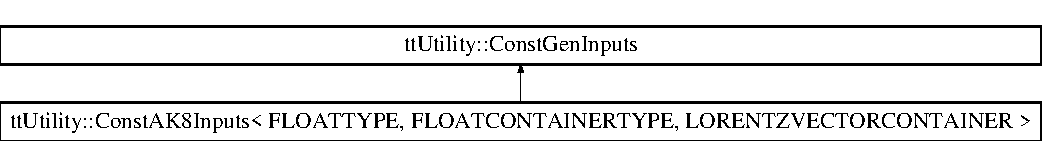
\includegraphics[height=2.000000cm]{classttUtility_1_1ConstAK8Inputs}
\end{center}
\end{figure}
\subsection*{Public Member Functions}
\begin{DoxyCompactItemize}
\item 
\hypertarget{classttUtility_1_1ConstAK8Inputs_a0f8cfcf1305dd45f8694d1d4172f2766}{{\bfseries Const\-A\-K8\-Inputs} (const std\-::vector$<$ T\-Lorentz\-Vector $>$ \&jets\-L\-Vec, const std\-::vector$<$ double $>$ \&tau1, const std\-::vector$<$ double $>$ \&tau2, const std\-::vector$<$ double $>$ \&tau3, const std\-::vector$<$ double $>$ \&soft\-Drop\-Mass, const std\-::vector$<$ T\-Lorentz\-Vector $>$ \&subjets\-L\-Vec)}\label{classttUtility_1_1ConstAK8Inputs_a0f8cfcf1305dd45f8694d1d4172f2766}

\item 
\hypertarget{classttUtility_1_1ConstAK8Inputs_a97223b6b84a2899e99fcb50d369b483d}{{\bfseries Const\-A\-K8\-Inputs} (const std\-::vector$<$ T\-Lorentz\-Vector $>$ \&jets\-L\-Vec, const std\-::vector$<$ double $>$ \&tau1, const std\-::vector$<$ double $>$ \&tau2, const std\-::vector$<$ double $>$ \&tau3, const std\-::vector$<$ double $>$ \&soft\-Drop\-Mass, const std\-::vector$<$ T\-Lorentz\-Vector $>$ \&subjets\-L\-Vec, const std\-::vector$<$ double $>$ \&subjets\-Btag, const std\-::vector$<$ double $>$ \&subjets\-Mult, const std\-::vector$<$ double $>$ \&subjets\-Pt\-D, const std\-::vector$<$ double $>$ \&subjets\-Axis1, const std\-::vector$<$ double $>$ \&subjets\-Axis2)}\label{classttUtility_1_1ConstAK8Inputs_a97223b6b84a2899e99fcb50d369b483d}

\item 
\hypertarget{classttUtility_1_1ConstAK8Inputs_a1a00ffaf521c7308969d6bf31fb683f4}{{\bfseries Const\-A\-K8\-Inputs} (const std\-::vector$<$ T\-Lorentz\-Vector $>$ \&jets\-L\-Vec, const std\-::vector$<$ double $>$ \&tau1, const std\-::vector$<$ double $>$ \&tau2, const std\-::vector$<$ double $>$ \&tau3, const std\-::vector$<$ double $>$ \&soft\-Drop\-Mass, const std\-::vector$<$ std\-::vector$<$ T\-Lorentz\-Vector $>$ $>$ \&vec\-Sub\-Jets\-L\-Vec)}\label{classttUtility_1_1ConstAK8Inputs_a1a00ffaf521c7308969d6bf31fb683f4}

\item 
\hypertarget{classttUtility_1_1ConstAK8Inputs_a2ac576a4f54d10d841172c34ed955f0c}{{\bfseries Const\-A\-K8\-Inputs} (const std\-::vector$<$ T\-Lorentz\-Vector $>$ \&jets\-L\-Vec, const std\-::vector$<$ double $>$ \&tau1, const std\-::vector$<$ double $>$ \&tau2, const std\-::vector$<$ double $>$ \&tau3, const std\-::vector$<$ double $>$ \&soft\-Drop\-Mass, const std\-::vector$<$ T\-Lorentz\-Vector $>$ \&subjets\-L\-Vec, const std\-::vector$<$ T\-Lorentz\-Vector $>$ \&had\-Gen\-Tops, const std\-::vector$<$ std\-::vector$<$ const T\-Lorentz\-Vector $\ast$ $>$$>$ \&had\-Gen\-Top\-Daughters)}\label{classttUtility_1_1ConstAK8Inputs_a2ac576a4f54d10d841172c34ed955f0c}

\item 
\hypertarget{classttUtility_1_1ConstAK8Inputs_a3383d6cf39e78b5cf3e36fe6b3b0664e}{{\bfseries Const\-A\-K8\-Inputs} (const std\-::vector$<$ T\-Lorentz\-Vector $>$ \&jets\-L\-Vec, const std\-::vector$<$ double $>$ \&tau1, const std\-::vector$<$ double $>$ \&tau2, const std\-::vector$<$ double $>$ \&tau3, const std\-::vector$<$ double $>$ \&soft\-Drop\-Mass, const std\-::vector$<$ T\-Lorentz\-Vector $>$ \&subjets\-L\-Vec, const std\-::vector$<$ double $>$ \&subjets\-Btag, const std\-::vector$<$ double $>$ \&subjets\-Mult, const std\-::vector$<$ double $>$ \&subjets\-Pt\-D, const std\-::vector$<$ double $>$ \&subjets\-Axis1, const std\-::vector$<$ double $>$ \&subjets\-Axis2, const std\-::vector$<$ T\-Lorentz\-Vector $>$ \&had\-Gen\-Tops, const std\-::vector$<$ std\-::vector$<$ const T\-Lorentz\-Vector $\ast$ $>$$>$ \&had\-Gen\-Top\-Daughters)}\label{classttUtility_1_1ConstAK8Inputs_a3383d6cf39e78b5cf3e36fe6b3b0664e}

\item 
\hypertarget{classttUtility_1_1ConstAK8Inputs_aded941e18d86f235e8e20101fda1e940}{{\bfseries Const\-A\-K8\-Inputs} (const std\-::vector$<$ T\-Lorentz\-Vector $>$ \&jets\-L\-Vec, const std\-::vector$<$ double $>$ \&tau1, const std\-::vector$<$ double $>$ \&tau2, const std\-::vector$<$ double $>$ \&tau3, const std\-::vector$<$ double $>$ \&soft\-Drop\-Mass, const std\-::vector$<$ std\-::vector$<$ T\-Lorentz\-Vector $>$ $>$ \&vec\-Sub\-Jets\-L\-Vec, const std\-::vector$<$ T\-Lorentz\-Vector $>$ \&had\-Gen\-Tops, const std\-::vector$<$ std\-::vector$<$ const T\-Lorentz\-Vector $\ast$ $>$$>$ \&had\-Gen\-Top\-Daughters)}\label{classttUtility_1_1ConstAK8Inputs_aded941e18d86f235e8e20101fda1e940}

\item 
\hypertarget{classttUtility_1_1ConstAK8Inputs_a8ed6e23d77aec6b257c6cd2c383e41a1}{void {\bfseries package\-Constituents} (std\-::vector$<$ \hyperlink{classConstituent}{Constituent} $>$ \&constituents)}\label{classttUtility_1_1ConstAK8Inputs_a8ed6e23d77aec6b257c6cd2c383e41a1}

\item 
\hypertarget{classttUtility_1_1ConstAK8Inputs_acf5080a09bbaf261d42cba91e6d5274a}{std\-::vector$<$ T\-Lorentz\-Vector $>$ {\bfseries denominator} (const double pt\-Cut) const }\label{classttUtility_1_1ConstAK8Inputs_acf5080a09bbaf261d42cba91e6d5274a}

\item 
\hypertarget{classttUtility_1_1ConstAK8Inputs_a331aa8e6bbefade26efd24be32ad1b5d}{void {\bfseries set\-W\-Mass\-Corr\-Histos} (const std\-::string \&fname)}\label{classttUtility_1_1ConstAK8Inputs_a331aa8e6bbefade26efd24be32ad1b5d}

\item 
\hypertarget{classttUtility_1_1ConstAK8Inputs_a64b27b878a5c341b37defe5637b554fc}{void {\bfseries set\-W\-Mass\-Corr\-Histos} (T\-F1 $\ast$puppisd\-\_\-corr\-G\-E\-N, T\-F1 $\ast$puppisd\-\_\-corr\-R\-E\-C\-O\-\_\-cen, T\-F1 $\ast$puppisd\-\_\-corr\-R\-E\-C\-O\-\_\-for)}\label{classttUtility_1_1ConstAK8Inputs_a64b27b878a5c341b37defe5637b554fc}

\end{DoxyCompactItemize}
\subsection*{Static Public Member Functions}
\begin{DoxyCompactItemize}
\item 
\hypertarget{classttUtility_1_1ConstAK8Inputs_a9f18c082d4f1a3f031b1b99ed0ab775f}{static void {\bfseries prep\-Histos\-For\-W\-Correction\-Factors} (const std\-::string \&fname, T\-F1 $\ast$puppisd\-\_\-corr\-G\-E\-N, T\-F1 $\ast$puppisd\-\_\-corr\-R\-E\-C\-O\-\_\-cen, T\-F1 $\ast$puppisd\-\_\-corr\-R\-E\-C\-O\-\_\-for)}\label{classttUtility_1_1ConstAK8Inputs_a9f18c082d4f1a3f031b1b99ed0ab775f}

\end{DoxyCompactItemize}
\subsection*{Additional Inherited Members}


\subsection{Detailed Description}
Class to gather the information necessary to construct the A\-K8 jet constituents 

The documentation for this class was generated from the following files\-:\begin{DoxyCompactItemize}
\item 
/home/travis/build/susy2015/\-Top\-Tagger/\-Top\-Tagger/include/\hyperlink{TopTaggerUtilities_8h}{Top\-Tagger\-Utilities.\-h}\item 
/home/travis/build/susy2015/\-Top\-Tagger/\-Top\-Tagger/src/Top\-Tagger\-Utilities.\-cpp\end{DoxyCompactItemize}

\hypertarget{classttUtility_1_1ConstGenInputs}{\section{tt\-Utility\-:\-:Const\-Gen\-Inputs Class Reference}
\label{classttUtility_1_1ConstGenInputs}\index{tt\-Utility\-::\-Const\-Gen\-Inputs@{tt\-Utility\-::\-Const\-Gen\-Inputs}}
}


{\ttfamily \#include $<$Top\-Tagger\-Utilities.\-h$>$}

Inheritance diagram for tt\-Utility\-:\-:Const\-Gen\-Inputs\-:\begin{figure}[H]
\begin{center}
\leavevmode
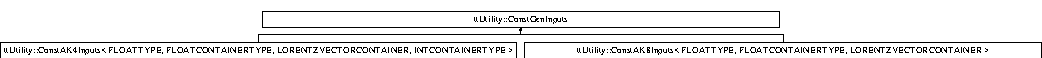
\includegraphics[height=2.000000cm]{classttUtility_1_1ConstGenInputs}
\end{center}
\end{figure}
\subsection*{Protected Member Functions}
\begin{DoxyCompactItemize}
\item 
\hypertarget{classttUtility_1_1ConstGenInputs_a520c5a594261d877f0fb4ad46aedc71e}{\hyperlink{classttUtility_1_1ConstGenInputs_a520c5a594261d877f0fb4ad46aedc71e}{Const\-Gen\-Inputs} ()}\label{classttUtility_1_1ConstGenInputs_a520c5a594261d877f0fb4ad46aedc71e}

\begin{DoxyCompactList}\small\item\em Default constructor. \end{DoxyCompactList}\item 
\hyperlink{classttUtility_1_1ConstGenInputs_a36cd5945c3febe03ded92e506d86e7c4}{Const\-Gen\-Inputs} (const std\-::vector$<$ T\-Lorentz\-Vector $>$ \&had\-Gen\-Tops, const std\-::vector$<$ std\-::vector$<$ const T\-Lorentz\-Vector $\ast$ $>$$>$ \&had\-Gen\-Top\-Daughters)
\end{DoxyCompactItemize}
\subsection*{Protected Attributes}
\begin{DoxyCompactItemize}
\item 
\hypertarget{classttUtility_1_1ConstGenInputs_aa81a1bd7a31b8a11ead74009bbfba1f0}{const std\-::vector\\*
$<$ T\-Lorentz\-Vector $>$ $\ast$ {\bfseries had\-Gen\-Tops\-\_\-}}\label{classttUtility_1_1ConstGenInputs_aa81a1bd7a31b8a11ead74009bbfba1f0}

\item 
\hypertarget{classttUtility_1_1ConstGenInputs_a87acbb7879cdbcb43b4f08adfe78d93e}{const std\-::vector$<$ std\-::vector\\*
$<$ const T\-Lorentz\-Vector $\ast$ $>$ $>$ $\ast$ {\bfseries had\-Gen\-Top\-Daughters\-\_\-}}\label{classttUtility_1_1ConstGenInputs_a87acbb7879cdbcb43b4f08adfe78d93e}

\end{DoxyCompactItemize}


\subsection{Detailed Description}
Class to hold the gen level inputs. 

\subsection{Constructor \& Destructor Documentation}
\hypertarget{classttUtility_1_1ConstGenInputs_a36cd5945c3febe03ded92e506d86e7c4}{\index{tt\-Utility\-::\-Const\-Gen\-Inputs@{tt\-Utility\-::\-Const\-Gen\-Inputs}!Const\-Gen\-Inputs@{Const\-Gen\-Inputs}}
\index{Const\-Gen\-Inputs@{Const\-Gen\-Inputs}!ttUtility::ConstGenInputs@{tt\-Utility\-::\-Const\-Gen\-Inputs}}
\subsubsection[{Const\-Gen\-Inputs}]{\setlength{\rightskip}{0pt plus 5cm}tt\-Utility\-::\-Const\-Gen\-Inputs\-::\-Const\-Gen\-Inputs (
\begin{DoxyParamCaption}
\item[{const std\-::vector$<$ T\-Lorentz\-Vector $>$ \&}]{had\-Gen\-Tops, }
\item[{const std\-::vector$<$ std\-::vector$<$ const T\-Lorentz\-Vector $\ast$ $>$$>$ \&}]{had\-Gen\-Top\-Daughters}
\end{DoxyParamCaption}
)\hspace{0.3cm}{\ttfamily [protected]}}}\label{classttUtility_1_1ConstGenInputs_a36cd5945c3febe03ded92e506d86e7c4}
Constructs gen inputs from gen level vectors 
\begin{DoxyParams}{Parameters}
{\em had\-Gen\-Tops} & Vector of hadronicly decaying gen top T\-Lorentz\-Vectors \\
\hline
{\em had\-Gen\-Top\-Daughters} & Vector of direct decay daughters of the top quarks \\
\hline
\end{DoxyParams}


The documentation for this class was generated from the following files\-:\begin{DoxyCompactItemize}
\item 
/home/travis/build/susy2015/\-Top\-Tagger/\-Top\-Tagger/include/\hyperlink{TopTaggerUtilities_8h}{Top\-Tagger\-Utilities.\-h}\item 
/home/travis/build/susy2015/\-Top\-Tagger/\-Top\-Tagger/src/Top\-Tagger\-Utilities.\-cpp\end{DoxyCompactItemize}

\hypertarget{classConstituent}{\section{Constituent Class Reference}
\label{classConstituent}\index{Constituent@{Constituent}}
}


{\ttfamily \#include $<$Constituent.\-h$>$}

\subsection*{Public Member Functions}
\begin{DoxyCompactItemize}
\item 
\hyperlink{classConstituent_a70507cdd41d24d156a07bb9409bc95cf}{Constituent} ()
\item 
\hyperlink{classConstituent_a86026ceffb0b81b7f1b306474325789b}{Constituent} (const T\-Lorentz\-Vector \&\hyperlink{classConstituent_a3f918f1210cc666288327544e32d728c}{p}, const double \&b\-Tag\-Disc, const double \&qg\-Likelihood)
\item 
\hyperlink{classConstituent_a812c45810832e1098b6d21c6050c123a}{Constituent} (const T\-Lorentz\-Vector \&\hyperlink{classConstituent_a3f918f1210cc666288327544e32d728c}{p}, const Constituent\-Type \&type)
\item 
\hyperlink{classConstituent_aea65c8ccaa87cd41431adeabdd667c7b}{Constituent} (const T\-Lorentz\-Vector \&\hyperlink{classConstituent_a3f918f1210cc666288327544e32d728c}{p}, const double \&tau1, const double \&tau2, const double \&tau3, const double \&soft\-Drop\-Mass, const std\-::vector$<$ \hyperlink{classConstituent}{Constituent} $>$ \&subjets, const double \&w\-Mass\-Corr)
\item 
\hypertarget{classConstituent_a5282e40233ba506ee9a1e8a5c423ecd3}{void {\bfseries set\-P\-Btag} (const T\-Lorentz\-Vector \&\hyperlink{classConstituent_a3f918f1210cc666288327544e32d728c}{p}, const double \&b\-Tag\-Disc, const double \&qg\-Likelihood)}\label{classConstituent_a5282e40233ba506ee9a1e8a5c423ecd3}

\item 
\hypertarget{classConstituent_a047ea32763c043302815face1f3aef35}{void {\bfseries set\-P} (const T\-Lorentz\-Vector \&\hyperlink{classConstituent_a3f918f1210cc666288327544e32d728c}{p})}\label{classConstituent_a047ea32763c043302815face1f3aef35}

\item 
\hypertarget{classConstituent_ad3e78cbae563a423c7d31aa5d9ca4a30}{void {\bfseries set\-B\-Tag} (const double \&b\-Tag\-Disc)}\label{classConstituent_ad3e78cbae563a423c7d31aa5d9ca4a30}

\item 
\hypertarget{classConstituent_a8d08fcf43d1d33d4a09854b3a180499b}{void {\bfseries set\-Q\-G\-Likelihood} (const double \&qg\-Likelihood)}\label{classConstituent_a8d08fcf43d1d33d4a09854b3a180499b}

\item 
\hypertarget{classConstituent_addfb4fd94597fee1886d4673256d4835}{void {\bfseries set\-Type} (const Constituent\-Type type)}\label{classConstituent_addfb4fd94597fee1886d4673256d4835}

\item 
\hypertarget{classConstituent_a9d1493cc1e27c929833f5d98b73ddd88}{void {\bfseries set\-Tau1} (const double \&tau1)}\label{classConstituent_a9d1493cc1e27c929833f5d98b73ddd88}

\item 
\hypertarget{classConstituent_ae090779940f2716959ece7eacd94030d}{void {\bfseries set\-Tau2} (const double \&tau2)}\label{classConstituent_ae090779940f2716959ece7eacd94030d}

\item 
\hypertarget{classConstituent_a3e08a3c5233f6cb754404e73e25b1a8c}{void {\bfseries set\-Tau3} (const double \&tau3)}\label{classConstituent_a3e08a3c5233f6cb754404e73e25b1a8c}

\item 
\hypertarget{classConstituent_abacfdb87d076479f5a5dab8147ca2bb3}{void {\bfseries set\-Soft\-Drop\-Mass} (const double \&soft\-Drop\-Mass)}\label{classConstituent_abacfdb87d076479f5a5dab8147ca2bb3}

\item 
\hypertarget{classConstituent_a80a81bb60ea3ed312e058e46b53ff791}{void {\bfseries set\-Sub\-Jets} (const std\-::vector$<$ \hyperlink{classConstituent}{Constituent} $>$ \&subjets)}\label{classConstituent_a80a81bb60ea3ed312e058e46b53ff791}

\item 
\hypertarget{classConstituent_a934831e1872c7ac6f1e777d3069ee55a}{void {\bfseries set\-Q\-G\-L\-Vars} (const double qg\-Mult, const double qg\-Pt\-D, const double qg\-Axis1, const double qg\-Axis2)}\label{classConstituent_a934831e1872c7ac6f1e777d3069ee55a}

\item 
\hypertarget{classConstituent_ac8ce2c1a6eb317adc0d371f5ef49c726}{void {\bfseries set\-W\-Mass\-Corr} (const double \&w\-Mass\-Corr)}\label{classConstituent_ac8ce2c1a6eb317adc0d371f5ef49c726}

\item 
\hypertarget{classConstituent_a61c3073e6ed0f3d5c93c9d8289453cb9}{void {\bfseries set\-Top\-Disc} (const double \&top\-Disc)}\label{classConstituent_a61c3073e6ed0f3d5c93c9d8289453cb9}

\item 
\hypertarget{classConstituent_a48d0d129c41154c3dcaa51ff3e5c44c3}{void {\bfseries set\-W\-Disc} (const double \&W\-Disc)}\label{classConstituent_a48d0d129c41154c3dcaa51ff3e5c44c3}

\item 
\hypertarget{classConstituent_abc67caff918e263ec1e58372efa4641b}{void {\bfseries set\-Index} (const unsigned int \&index)}\label{classConstituent_abc67caff918e263ec1e58372efa4641b}

\item 
void \hyperlink{classConstituent_a1b2fc086bc359e141e54ed2903c951c9}{set\-Extra\-Var} (const std\-::string \&name, const double var)
\item 
void \hyperlink{classConstituent_a2aea6bdc5229bb87227bcc8caa9c51c6}{add\-Gen\-Match} (const T\-Lorentz\-Vector \&gen\-Top, const T\-Lorentz\-Vector $\ast$gen\-Daughter)
\item 
const T\-Lorentz\-Vector \& \hyperlink{classConstituent_a3f918f1210cc666288327544e32d728c}{p} () const 
\item 
const T\-Lorentz\-Vector \& \hyperlink{classConstituent_a9f95db0ef9ae97fa0dc2cf45153e4131}{P} () const 
\item 
\hypertarget{classConstituent_ac4954793667cf0b2ffd136fbd8df0cda}{const T\-Lorentz\-Vector \& {\bfseries get\-P} () const }\label{classConstituent_ac4954793667cf0b2ffd136fbd8df0cda}

\item 
\hypertarget{classConstituent_af2cbdf02c47682a97db91a724a4ae3e1}{double {\bfseries get\-B\-Tag\-Disc} () const }\label{classConstituent_af2cbdf02c47682a97db91a724a4ae3e1}

\item 
\hypertarget{classConstituent_ae58e807a0bd4adfff6c052882f2f9396}{double {\bfseries get\-Q\-G\-Likelihood} () const }\label{classConstituent_ae58e807a0bd4adfff6c052882f2f9396}

\item 
\hypertarget{classConstituent_a325cb683912acb64e2fcbde14726f6a6}{Constituent\-Type {\bfseries get\-Type} () const }\label{classConstituent_a325cb683912acb64e2fcbde14726f6a6}

\item 
\hypertarget{classConstituent_a2c057eb66cfeed68e5bd58e1c5815e8b}{double {\bfseries get\-Tau1} () const }\label{classConstituent_a2c057eb66cfeed68e5bd58e1c5815e8b}

\item 
\hypertarget{classConstituent_aa43ea922dc8db06b1b28b8a66db0edac}{double {\bfseries get\-Tau2} () const }\label{classConstituent_aa43ea922dc8db06b1b28b8a66db0edac}

\item 
\hypertarget{classConstituent_ac33bc6f45eca6ce4fc6f5cef83159156}{double {\bfseries get\-Tau3} () const }\label{classConstituent_ac33bc6f45eca6ce4fc6f5cef83159156}

\item 
\hypertarget{classConstituent_a0aa688482470252d075d07e9467e21c0}{double {\bfseries get\-Soft\-Drop\-Mass} () const }\label{classConstituent_a0aa688482470252d075d07e9467e21c0}

\item 
\hypertarget{classConstituent_a07f258d8045b1dc37fecf10b44448ba4}{decltype(subjets\-\_\-) const \& {\bfseries get\-Subjets} () const }\label{classConstituent_a07f258d8045b1dc37fecf10b44448ba4}

\item 
\hypertarget{classConstituent_a228e250e72e942fdea1681b410f4678d}{decltype(gen\-Matches\-\_\-) const \& {\bfseries get\-Gen\-Matches} () const }\label{classConstituent_a228e250e72e942fdea1681b410f4678d}

\item 
\hypertarget{classConstituent_a01bc43e8507edb0dd049a0116ce1eb2f}{double {\bfseries get\-W\-Mass\-Corr} () const }\label{classConstituent_a01bc43e8507edb0dd049a0116ce1eb2f}

\item 
\hypertarget{classConstituent_aac16a1b470590029529d1a6b77d50f41}{double {\bfseries get\-Q\-G\-Mult} () const }\label{classConstituent_aac16a1b470590029529d1a6b77d50f41}

\item 
\hypertarget{classConstituent_a088fc8a7a9324cd7568c47d96a3d08db}{double {\bfseries get\-Q\-G\-Pt\-D} () const }\label{classConstituent_a088fc8a7a9324cd7568c47d96a3d08db}

\item 
\hypertarget{classConstituent_a6120efae2154ff7167e70e32a260fed8}{double {\bfseries get\-Q\-G\-Axis1} () const }\label{classConstituent_a6120efae2154ff7167e70e32a260fed8}

\item 
\hypertarget{classConstituent_a26c8c9244eda89d85a0441bf71a7e21e}{double {\bfseries get\-Q\-G\-Axis2} () const }\label{classConstituent_a26c8c9244eda89d85a0441bf71a7e21e}

\item 
\hypertarget{classConstituent_a5e6d49f8b60711586aed4506a07b538c}{double {\bfseries get\-Top\-Disc} () const }\label{classConstituent_a5e6d49f8b60711586aed4506a07b538c}

\item 
\hypertarget{classConstituent_a9184e1d6ed1691f6efd0c5083444c021}{double {\bfseries get\-W\-Disc} () const }\label{classConstituent_a9184e1d6ed1691f6efd0c5083444c021}

\item 
\hypertarget{classConstituent_a64e38c0209bf5198477160ea690bbaf9}{int {\bfseries get\-Index} () const }\label{classConstituent_a64e38c0209bf5198477160ea690bbaf9}

\item 
double \hyperlink{classConstituent_a8fc04ce34e4e9c162f3d02f62f6b50cb}{get\-Extra\-Var} (const std\-::string var) const 
\end{DoxyCompactItemize}


\subsection{Detailed Description}
Serves as a container class for jet objects including the 4-\/vector for each jet along with supporting information such as the b-\/tag discriminator and jet type 

\subsection{Constructor \& Destructor Documentation}
\hypertarget{classConstituent_a70507cdd41d24d156a07bb9409bc95cf}{\index{Constituent@{Constituent}!Constituent@{Constituent}}
\index{Constituent@{Constituent}!Constituent@{Constituent}}
\subsubsection[{Constituent}]{\setlength{\rightskip}{0pt plus 5cm}Constituent\-::\-Constituent (
\begin{DoxyParamCaption}
{}
\end{DoxyParamCaption}
)}}\label{classConstituent_a70507cdd41d24d156a07bb9409bc95cf}
Empty constructor \hypertarget{classConstituent_a86026ceffb0b81b7f1b306474325789b}{\index{Constituent@{Constituent}!Constituent@{Constituent}}
\index{Constituent@{Constituent}!Constituent@{Constituent}}
\subsubsection[{Constituent}]{\setlength{\rightskip}{0pt plus 5cm}Constituent\-::\-Constituent (
\begin{DoxyParamCaption}
\item[{const T\-Lorentz\-Vector \&}]{p, }
\item[{const double \&}]{b\-Tag\-Disc, }
\item[{const double \&}]{qg\-Likelihood}
\end{DoxyParamCaption}
)}}\label{classConstituent_a86026ceffb0b81b7f1b306474325789b}
Construct an A\-K4 jet from T\-Lorentz\-Vector, b-\/tag discriminator, and quark-\/gluonlikelihood \hypertarget{classConstituent_a812c45810832e1098b6d21c6050c123a}{\index{Constituent@{Constituent}!Constituent@{Constituent}}
\index{Constituent@{Constituent}!Constituent@{Constituent}}
\subsubsection[{Constituent}]{\setlength{\rightskip}{0pt plus 5cm}Constituent\-::\-Constituent (
\begin{DoxyParamCaption}
\item[{const T\-Lorentz\-Vector \&}]{p, }
\item[{const Constituent\-Type \&}]{type}
\end{DoxyParamCaption}
)}}\label{classConstituent_a812c45810832e1098b6d21c6050c123a}
Construct generic constituent jet from T\-Lorentz\-Vector and type \hypertarget{classConstituent_aea65c8ccaa87cd41431adeabdd667c7b}{\index{Constituent@{Constituent}!Constituent@{Constituent}}
\index{Constituent@{Constituent}!Constituent@{Constituent}}
\subsubsection[{Constituent}]{\setlength{\rightskip}{0pt plus 5cm}Constituent\-::\-Constituent (
\begin{DoxyParamCaption}
\item[{const T\-Lorentz\-Vector \&}]{p, }
\item[{const double \&}]{tau1, }
\item[{const double \&}]{tau2, }
\item[{const double \&}]{tau3, }
\item[{const double \&}]{soft\-Drop\-Mass, }
\item[{const std\-::vector$<$ {\bf Constituent} $>$ \&}]{subjets, }
\item[{const double \&}]{w\-Mass\-Corr}
\end{DoxyParamCaption}
)}}\label{classConstituent_aea65c8ccaa87cd41431adeabdd667c7b}
Construct an A\-K8 jet from T\-Lorentz\-Vector, Nsubjettiness inputs tau1/2/3, softdrop mass, softdrop subjets vector and w\-Mass\-Correction (if applicable). 

\subsection{Member Function Documentation}
\hypertarget{classConstituent_a2aea6bdc5229bb87227bcc8caa9c51c6}{\index{Constituent@{Constituent}!add\-Gen\-Match@{add\-Gen\-Match}}
\index{add\-Gen\-Match@{add\-Gen\-Match}!Constituent@{Constituent}}
\subsubsection[{add\-Gen\-Match}]{\setlength{\rightskip}{0pt plus 5cm}void Constituent\-::add\-Gen\-Match (
\begin{DoxyParamCaption}
\item[{const T\-Lorentz\-Vector \&}]{gen\-Top, }
\item[{const T\-Lorentz\-Vector $\ast$}]{gen\-Daughter}
\end{DoxyParamCaption}
)}}\label{classConstituent_a2aea6bdc5229bb87227bcc8caa9c51c6}
Add a generator level matched particle 
\begin{DoxyParams}[1]{Parameters}
\mbox{\tt in}  & {\em gen\-Top} & T\-Lorentz\-Vector of the generator top \\
\hline
\mbox{\tt in}  & {\em gen\-Daughter} & T\-Lorentz\-Vector of the generator level daughter directly matched to the constituent \\
\hline
\end{DoxyParams}
\hypertarget{classConstituent_a8fc04ce34e4e9c162f3d02f62f6b50cb}{\index{Constituent@{Constituent}!get\-Extra\-Var@{get\-Extra\-Var}}
\index{get\-Extra\-Var@{get\-Extra\-Var}!Constituent@{Constituent}}
\subsubsection[{get\-Extra\-Var}]{\setlength{\rightskip}{0pt plus 5cm}double Constituent\-::get\-Extra\-Var (
\begin{DoxyParamCaption}
\item[{const std\-::string}]{var}
\end{DoxyParamCaption}
) const}}\label{classConstituent_a8fc04ce34e4e9c162f3d02f62f6b50cb}
Retrieve an extra variable based upon its name 
\begin{DoxyParams}[1]{Parameters}
\mbox{\tt in}  & {\em var} & Name of the variable to retrieve \\
\hline
\end{DoxyParams}
\begin{DoxyReturn}{Returns}
Value of the variable 
\end{DoxyReturn}
\hypertarget{classConstituent_a3f918f1210cc666288327544e32d728c}{\index{Constituent@{Constituent}!p@{p}}
\index{p@{p}!Constituent@{Constituent}}
\subsubsection[{p}]{\setlength{\rightskip}{0pt plus 5cm}const T\-Lorentz\-Vector\& Constituent\-::p (
\begin{DoxyParamCaption}
{}
\end{DoxyParamCaption}
) const\hspace{0.3cm}{\ttfamily [inline]}}}\label{classConstituent_a3f918f1210cc666288327544e32d728c}
\begin{DoxyReturn}{Returns}
\hyperlink{classConstituent}{Constituent} T\-Lorentz\-Vector 
\end{DoxyReturn}
\hypertarget{classConstituent_a9f95db0ef9ae97fa0dc2cf45153e4131}{\index{Constituent@{Constituent}!P@{P}}
\index{P@{P}!Constituent@{Constituent}}
\subsubsection[{P}]{\setlength{\rightskip}{0pt plus 5cm}const T\-Lorentz\-Vector\& Constituent\-::\-P (
\begin{DoxyParamCaption}
{}
\end{DoxyParamCaption}
) const\hspace{0.3cm}{\ttfamily [inline]}}}\label{classConstituent_a9f95db0ef9ae97fa0dc2cf45153e4131}
Alias for \hyperlink{classConstituent_a3f918f1210cc666288327544e32d728c}{p()} \hypertarget{classConstituent_a1b2fc086bc359e141e54ed2903c951c9}{\index{Constituent@{Constituent}!set\-Extra\-Var@{set\-Extra\-Var}}
\index{set\-Extra\-Var@{set\-Extra\-Var}!Constituent@{Constituent}}
\subsubsection[{set\-Extra\-Var}]{\setlength{\rightskip}{0pt plus 5cm}void Constituent\-::set\-Extra\-Var (
\begin{DoxyParamCaption}
\item[{const std\-::string \&}]{name, }
\item[{const double}]{var}
\end{DoxyParamCaption}
)}}\label{classConstituent_a1b2fc086bc359e141e54ed2903c951c9}
Adds an extra variable which is not included in the primary members of the \hyperlink{classConstituent}{Constituent} class. These will be added and retrieved by name. 
\begin{DoxyParams}[1]{Parameters}
\mbox{\tt in}  & {\em name} & Name used to store the parameter \\
\hline
\mbox{\tt in}  & {\em var} & Value of the parameter \\
\hline
\end{DoxyParams}


The documentation for this class was generated from the following files\-:\begin{DoxyCompactItemize}
\item 
/home/travis/build/susy2015/\-Top\-Tagger/\-Top\-Tagger/include/Constituent.\-h\item 
/home/travis/build/susy2015/\-Top\-Tagger/\-Top\-Tagger/src/Constituent.\-cpp\end{DoxyCompactItemize}

\hypertarget{classttUtility_1_1ConstResolvedCandInputs}{\section{tt\-Utility\-:\-:Const\-Resolved\-Cand\-Inputs$<$ F\-L\-O\-A\-T\-T\-Y\-P\-E, F\-L\-O\-A\-T\-C\-O\-N\-T\-A\-I\-N\-E\-R\-T\-Y\-P\-E, I\-N\-T\-C\-O\-N\-T\-A\-I\-N\-E\-R\-T\-Y\-P\-E, L\-O\-R\-E\-N\-T\-Z\-V\-E\-C\-T\-O\-R\-C\-O\-N\-T\-A\-I\-N\-E\-R $>$ Class Template Reference}
\label{classttUtility_1_1ConstResolvedCandInputs}\index{tt\-Utility\-::\-Const\-Resolved\-Cand\-Inputs$<$ F\-L\-O\-A\-T\-T\-Y\-P\-E, F\-L\-O\-A\-T\-C\-O\-N\-T\-A\-I\-N\-E\-R\-T\-Y\-P\-E, I\-N\-T\-C\-O\-N\-T\-A\-I\-N\-E\-R\-T\-Y\-P\-E, L\-O\-R\-E\-N\-T\-Z\-V\-E\-C\-T\-O\-R\-C\-O\-N\-T\-A\-I\-N\-E\-R $>$@{tt\-Utility\-::\-Const\-Resolved\-Cand\-Inputs$<$ F\-L\-O\-A\-T\-T\-Y\-P\-E, F\-L\-O\-A\-T\-C\-O\-N\-T\-A\-I\-N\-E\-R\-T\-Y\-P\-E, I\-N\-T\-C\-O\-N\-T\-A\-I\-N\-E\-R\-T\-Y\-P\-E, L\-O\-R\-E\-N\-T\-Z\-V\-E\-C\-T\-O\-R\-C\-O\-N\-T\-A\-I\-N\-E\-R $>$}}
}


{\ttfamily \#include $<$Top\-Tagger\-Utilities.\-h$>$}

\subsection*{Public Member Functions}
\begin{DoxyCompactItemize}
\item 
\hyperlink{classttUtility_1_1ConstResolvedCandInputs_a7478c472a557e444c5de4f17fd29fa22}{Const\-Resolved\-Cand\-Inputs} (const L\-O\-R\-E\-N\-T\-Z\-V\-E\-C\-T\-O\-R\-C\-O\-N\-T\-A\-I\-N\-E\-R \&top\-Cand\-L\-Vec, const F\-L\-O\-A\-T\-C\-O\-N\-T\-A\-I\-N\-E\-R\-T\-Y\-P\-E \&top\-Cand\-Disc, const I\-N\-T\-C\-O\-N\-T\-A\-I\-N\-E\-R\-T\-Y\-P\-E \&top\-Cand\-J1, const I\-N\-T\-C\-O\-N\-T\-A\-I\-N\-E\-R\-T\-Y\-P\-E \&top\-Cand\-J2, const I\-N\-T\-C\-O\-N\-T\-A\-I\-N\-E\-R\-T\-Y\-P\-E \&top\-Cand\-J3)
\item 
void \hyperlink{classttUtility_1_1ConstResolvedCandInputs_a064297d644dcf43301fcb74dc6ba299f}{package\-Constituents} (std\-::vector$<$ \hyperlink{classConstituent}{Constituent} $>$ \&constituents)
\end{DoxyCompactItemize}


\subsection{Detailed Description}
\subsubsection*{template$<$typename F\-L\-O\-A\-T\-T\-Y\-P\-E, typename F\-L\-O\-A\-T\-C\-O\-N\-T\-A\-I\-N\-E\-R\-T\-Y\-P\-E = std\-::vector$<$\-F\-L\-O\-A\-T\-T\-Y\-P\-E$>$, typename I\-N\-T\-C\-O\-N\-T\-A\-I\-N\-E\-R\-T\-Y\-P\-E = std\-::vector$<$int$>$, typename L\-O\-R\-E\-N\-T\-Z\-V\-E\-C\-T\-O\-R\-C\-O\-N\-T\-A\-I\-N\-E\-R = std\-::vector$<$\-T\-Lorentz\-Vector$>$$>$class tt\-Utility\-::\-Const\-Resolved\-Cand\-Inputs$<$ F\-L\-O\-A\-T\-T\-Y\-P\-E, F\-L\-O\-A\-T\-C\-O\-N\-T\-A\-I\-N\-E\-R\-T\-Y\-P\-E, I\-N\-T\-C\-O\-N\-T\-A\-I\-N\-E\-R\-T\-Y\-P\-E, L\-O\-R\-E\-N\-T\-Z\-V\-E\-C\-T\-O\-R\-C\-O\-N\-T\-A\-I\-N\-E\-R $>$}

Class to gather the information necessary to construct the Resolved\-Top\-Cand Constituents 

\subsection{Constructor \& Destructor Documentation}
\hypertarget{classttUtility_1_1ConstResolvedCandInputs_a7478c472a557e444c5de4f17fd29fa22}{\index{tt\-Utility\-::\-Const\-Resolved\-Cand\-Inputs@{tt\-Utility\-::\-Const\-Resolved\-Cand\-Inputs}!Const\-Resolved\-Cand\-Inputs@{Const\-Resolved\-Cand\-Inputs}}
\index{Const\-Resolved\-Cand\-Inputs@{Const\-Resolved\-Cand\-Inputs}!ttUtility::ConstResolvedCandInputs@{tt\-Utility\-::\-Const\-Resolved\-Cand\-Inputs}}
\subsubsection[{Const\-Resolved\-Cand\-Inputs}]{\setlength{\rightskip}{0pt plus 5cm}template$<$typename F\-L\-O\-A\-T\-T\-Y\-P\-E , typename F\-L\-O\-A\-T\-C\-O\-N\-T\-A\-I\-N\-E\-R\-T\-Y\-P\-E  = std\-::vector$<$\-F\-L\-O\-A\-T\-T\-Y\-P\-E$>$, typename I\-N\-T\-C\-O\-N\-T\-A\-I\-N\-E\-R\-T\-Y\-P\-E  = std\-::vector$<$int$>$, typename L\-O\-R\-E\-N\-T\-Z\-V\-E\-C\-T\-O\-R\-C\-O\-N\-T\-A\-I\-N\-E\-R  = std\-::vector$<$\-T\-Lorentz\-Vector$>$$>$ {\bf tt\-Utility\-::\-Const\-Resolved\-Cand\-Inputs}$<$ F\-L\-O\-A\-T\-T\-Y\-P\-E, F\-L\-O\-A\-T\-C\-O\-N\-T\-A\-I\-N\-E\-R\-T\-Y\-P\-E, I\-N\-T\-C\-O\-N\-T\-A\-I\-N\-E\-R\-T\-Y\-P\-E, L\-O\-R\-E\-N\-T\-Z\-V\-E\-C\-T\-O\-R\-C\-O\-N\-T\-A\-I\-N\-E\-R $>$\-::{\bf Const\-Resolved\-Cand\-Inputs} (
\begin{DoxyParamCaption}
\item[{const L\-O\-R\-E\-N\-T\-Z\-V\-E\-C\-T\-O\-R\-C\-O\-N\-T\-A\-I\-N\-E\-R \&}]{top\-Cand\-L\-Vec, }
\item[{const F\-L\-O\-A\-T\-C\-O\-N\-T\-A\-I\-N\-E\-R\-T\-Y\-P\-E \&}]{top\-Cand\-Disc, }
\item[{const I\-N\-T\-C\-O\-N\-T\-A\-I\-N\-E\-R\-T\-Y\-P\-E \&}]{top\-Cand\-J1, }
\item[{const I\-N\-T\-C\-O\-N\-T\-A\-I\-N\-E\-R\-T\-Y\-P\-E \&}]{top\-Cand\-J2, }
\item[{const I\-N\-T\-C\-O\-N\-T\-A\-I\-N\-E\-R\-T\-Y\-P\-E \&}]{top\-Cand\-J3}
\end{DoxyParamCaption}
)\hspace{0.3cm}{\ttfamily [inline]}}}\label{classttUtility_1_1ConstResolvedCandInputs_a7478c472a557e444c5de4f17fd29fa22}
Basic constructor 
\begin{DoxyParams}{Parameters}
{\em top\-Cand\-L\-Vec} & Vector of lorentz vectors of resolved top candidates \\
\hline
{\em top\-Cand\-Disc} & Vector of discriminator values for resolved top candidates \\
\hline
{\em top\-Cand\-J1} & Vector of jet 1 indices for resolved top candidates, referenced with respect to the A\-K4 constituents \\
\hline
{\em top\-Cand\-J2} & Vector of jet 2 indices for resolved top candidates, referenced with respect to the A\-K4 constituents \\
\hline
{\em top\-Cand\-J3} & Vector of jet 3 indices for resolved top candidates, referenced with respect to the A\-K4 constituents \\
\hline
\end{DoxyParams}


\subsection{Member Function Documentation}
\hypertarget{classttUtility_1_1ConstResolvedCandInputs_a064297d644dcf43301fcb74dc6ba299f}{\index{tt\-Utility\-::\-Const\-Resolved\-Cand\-Inputs@{tt\-Utility\-::\-Const\-Resolved\-Cand\-Inputs}!package\-Constituents@{package\-Constituents}}
\index{package\-Constituents@{package\-Constituents}!ttUtility::ConstResolvedCandInputs@{tt\-Utility\-::\-Const\-Resolved\-Cand\-Inputs}}
\subsubsection[{package\-Constituents}]{\setlength{\rightskip}{0pt plus 5cm}template$<$typename F\-L\-O\-A\-T\-T\-Y\-P\-E , typename F\-L\-O\-A\-T\-C\-O\-N\-T\-A\-I\-N\-E\-R\-T\-Y\-P\-E  = std\-::vector$<$\-F\-L\-O\-A\-T\-T\-Y\-P\-E$>$, typename I\-N\-T\-C\-O\-N\-T\-A\-I\-N\-E\-R\-T\-Y\-P\-E  = std\-::vector$<$int$>$, typename L\-O\-R\-E\-N\-T\-Z\-V\-E\-C\-T\-O\-R\-C\-O\-N\-T\-A\-I\-N\-E\-R  = std\-::vector$<$\-T\-Lorentz\-Vector$>$$>$ void {\bf tt\-Utility\-::\-Const\-Resolved\-Cand\-Inputs}$<$ F\-L\-O\-A\-T\-T\-Y\-P\-E, F\-L\-O\-A\-T\-C\-O\-N\-T\-A\-I\-N\-E\-R\-T\-Y\-P\-E, I\-N\-T\-C\-O\-N\-T\-A\-I\-N\-E\-R\-T\-Y\-P\-E, L\-O\-R\-E\-N\-T\-Z\-V\-E\-C\-T\-O\-R\-C\-O\-N\-T\-A\-I\-N\-E\-R $>$\-::package\-Constituents (
\begin{DoxyParamCaption}
\item[{std\-::vector$<$ {\bf Constituent} $>$ \&}]{constituents}
\end{DoxyParamCaption}
)\hspace{0.3cm}{\ttfamily [inline]}}}\label{classttUtility_1_1ConstResolvedCandInputs_a064297d644dcf43301fcb74dc6ba299f}
Called to fill the constituents using the information collected in the class. Not intended to be called directly. 
\begin{DoxyParams}{Parameters}
{\em constituents} & vector to insert resolved top candidate constituents into \\
\hline
\end{DoxyParams}


The documentation for this class was generated from the following file\-:\begin{DoxyCompactItemize}
\item 
/home/travis/build/susy2015/\-Top\-Tagger/\-Top\-Tagger/interface/\hyperlink{TopTaggerUtilities_8h}{Top\-Tagger\-Utilities.\-h}\end{DoxyCompactItemize}

\hypertarget{classcfg_1_1Context}{\section{cfg\-:\-:Context Class Reference}
\label{classcfg_1_1Context}\index{cfg\-::\-Context@{cfg\-::\-Context}}
}
\subsection*{Public Types}
\begin{DoxyCompactItemize}
\item 
\hypertarget{classcfg_1_1Context_a2795b6ffdf6481f708701e2233a574d2}{typedef std\-::map$<$ std\-::string, \\*
\hyperlink{classcfg_1_1Literal}{Literal} $>$\-::const\-\_\-iterator {\bfseries const\-\_\-feature\-\_\-iterator}}\label{classcfg_1_1Context_a2795b6ffdf6481f708701e2233a574d2}

\end{DoxyCompactItemize}
\subsection*{Public Member Functions}
\begin{DoxyCompactItemize}
\item 
\hypertarget{classcfg_1_1Context_a0bf621792bb3954f475b2bbe6c69f6b9}{{\bfseries Context} (const std\-::string \&namesp)}\label{classcfg_1_1Context_a0bf621792bb3954f475b2bbe6c69f6b9}

\item 
\hypertarget{classcfg_1_1Context_a648f69ee38af881ca2146ee0165305c4}{{\bfseries Context} (const \hyperlink{classcfg_1_1Context}{Context} \&cxt)}\label{classcfg_1_1Context_a648f69ee38af881ca2146ee0165305c4}

\item 
\hypertarget{classcfg_1_1Context_ae983a160273978702ced02fa2dbe427a}{\hyperlink{classcfg_1_1Context}{Context} \& {\bfseries operator=} (const \hyperlink{classcfg_1_1Context}{Context} \&cxt)}\label{classcfg_1_1Context_ae983a160273978702ced02fa2dbe427a}

\item 
\hypertarget{classcfg_1_1Context_a7f9e49a8635fd52a86d62f4782510930}{std\-::string \hyperlink{classcfg_1_1Context_a7f9e49a8635fd52a86d62f4782510930}{ns} () const }\label{classcfg_1_1Context_a7f9e49a8635fd52a86d62f4782510930}

\begin{DoxyCompactList}\small\item\em get the namespace \end{DoxyCompactList}\item 
\hypertarget{classcfg_1_1Context_af1ab6523fda2781a6d7d3316fea68fe8}{void \hyperlink{classcfg_1_1Context_af1ab6523fda2781a6d7d3316fea68fe8}{set} (const std\-::string \&name, const std\-::string \&value)}\label{classcfg_1_1Context_af1ab6523fda2781a6d7d3316fea68fe8}

\begin{DoxyCompactList}\small\item\em set a feature of the namespace (string) \end{DoxyCompactList}\item 
\hypertarget{classcfg_1_1Context_a983796d226d2d2deab971f354b2ac649}{void \hyperlink{classcfg_1_1Context_a983796d226d2d2deab971f354b2ac649}{set} (const std\-::string \&name, const char $\ast$value)}\label{classcfg_1_1Context_a983796d226d2d2deab971f354b2ac649}

\begin{DoxyCompactList}\small\item\em set a feature of the namespace (string) \end{DoxyCompactList}\item 
\hypertarget{classcfg_1_1Context_a06edab7e54985b14fea0e088859f2c4b}{void \hyperlink{classcfg_1_1Context_a06edab7e54985b14fea0e088859f2c4b}{set} (const std\-::string \&name, int value)}\label{classcfg_1_1Context_a06edab7e54985b14fea0e088859f2c4b}

\begin{DoxyCompactList}\small\item\em set a feature of the namespace (integer) \end{DoxyCompactList}\item 
\hypertarget{classcfg_1_1Context_a3dbae42248afdcc80c10cccf79f7ed88}{void \hyperlink{classcfg_1_1Context_a3dbae42248afdcc80c10cccf79f7ed88}{set} (const std\-::string \&name, bool value)}\label{classcfg_1_1Context_a3dbae42248afdcc80c10cccf79f7ed88}

\begin{DoxyCompactList}\small\item\em set a feature of the namespace (boolean) \end{DoxyCompactList}\item 
\hypertarget{classcfg_1_1Context_a4d183ca165e439f5f37c1ef8ac9f4aec}{void \hyperlink{classcfg_1_1Context_a4d183ca165e439f5f37c1ef8ac9f4aec}{unset} (const std\-::string \&name)}\label{classcfg_1_1Context_a4d183ca165e439f5f37c1ef8ac9f4aec}

\begin{DoxyCompactList}\small\item\em unset a feature of the namespace \end{DoxyCompactList}\item 
\hypertarget{classcfg_1_1Context_aee81f27c123da4e0dac4de50e68df4fe}{bool \hyperlink{classcfg_1_1Context_aee81f27c123da4e0dac4de50e68df4fe}{exists} (const std\-::string \&name) const }\label{classcfg_1_1Context_aee81f27c123da4e0dac4de50e68df4fe}

\begin{DoxyCompactList}\small\item\em does this feature exist? \end{DoxyCompactList}\item 
\hypertarget{classcfg_1_1Context_a603fe12c0b04a99aa59c6c2bc17b6152}{const \hyperlink{classcfg_1_1Literal}{Literal} \& \hyperlink{classcfg_1_1Context_a603fe12c0b04a99aa59c6c2bc17b6152}{get} (const std\-::string \&name) const }\label{classcfg_1_1Context_a603fe12c0b04a99aa59c6c2bc17b6152}

\begin{DoxyCompactList}\small\item\em access the requested feature \end{DoxyCompactList}\item 
\hypertarget{classcfg_1_1Context_adaf70b7fb48272eed2f9a0cb2006a483}{bool \hyperlink{classcfg_1_1Context_adaf70b7fb48272eed2f9a0cb2006a483}{operator==} (const \hyperlink{classcfg_1_1Context}{Context} \&c) const }\label{classcfg_1_1Context_adaf70b7fb48272eed2f9a0cb2006a483}

\begin{DoxyCompactList}\small\item\em equality test \end{DoxyCompactList}\item 
\hypertarget{classcfg_1_1Context_a73d0f54c4f2dec91050b6f87ff93e93b}{const\-\_\-feature\-\_\-iterator \hyperlink{classcfg_1_1Context_a73d0f54c4f2dec91050b6f87ff93e93b}{feature\-\_\-begin} () const }\label{classcfg_1_1Context_a73d0f54c4f2dec91050b6f87ff93e93b}

\begin{DoxyCompactList}\small\item\em iterate over features \end{DoxyCompactList}\item 
\hypertarget{classcfg_1_1Context_a81e81c5c13fef2656ea8843f0948a6f6}{const\-\_\-feature\-\_\-iterator \hyperlink{classcfg_1_1Context_a81e81c5c13fef2656ea8843f0948a6f6}{feature\-\_\-end} () const }\label{classcfg_1_1Context_a81e81c5c13fef2656ea8843f0948a6f6}

\begin{DoxyCompactList}\small\item\em iterate over features \end{DoxyCompactList}\end{DoxyCompactItemize}


The documentation for this class was generated from the following files\-:\begin{DoxyCompactItemize}
\item 
/home/travis/build/susy2015/\-Top\-Tagger/\-Cfg\-Parser/include/Context.\-hh\item 
/home/travis/build/susy2015/\-Top\-Tagger/\-Cfg\-Parser/src/Context.\-cc\end{DoxyCompactItemize}

\hypertarget{classCreateModel_1_1CreateModel}{\section{Create\-Model.\-Create\-Model Class Reference}
\label{classCreateModel_1_1CreateModel}\index{Create\-Model.\-Create\-Model@{Create\-Model.\-Create\-Model}}
}
\subsection*{Public Member Functions}
\begin{DoxyCompactItemize}
\item 
def \hyperlink{classCreateModel_1_1CreateModel_ae868f99ce147ab3b0ff73c515006ba16}{weight\-\_\-variable}
\item 
def \hyperlink{classCreateModel_1_1CreateModel_a9cd7bb38d38886a36f8036aec997b566}{bias\-\_\-variable}
\item 
\hypertarget{classCreateModel_1_1CreateModel_afe92bae79b5fd702e02a43a5936df994}{def {\bfseries create\-Recurent\-Layers}}\label{classCreateModel_1_1CreateModel_afe92bae79b5fd702e02a43a5936df994}

\item 
\hypertarget{classCreateModel_1_1CreateModel_ae75976731946bd47ca90a966f2a8e261}{def {\bfseries create\-Conv\-Layers}}\label{classCreateModel_1_1CreateModel_ae75976731946bd47ca90a966f2a8e261}

\item 
\hypertarget{classCreateModel_1_1CreateModel_a86e1bd0898957507096454cd034a89dc}{def {\bfseries create\-C\-N\-N\-R\-N\-N\-Layers}}\label{classCreateModel_1_1CreateModel_a86e1bd0898957507096454cd034a89dc}

\item 
\hypertarget{classCreateModel_1_1CreateModel_a34c6677df45275266012e10d36e0c9c2}{def {\bfseries gradient\-Reversal}}\label{classCreateModel_1_1CreateModel_a34c6677df45275266012e10d36e0c9c2}

\item 
\hypertarget{classCreateModel_1_1CreateModel_a0cec7ff4bfd516b73c48f92d321bd23d}{def {\bfseries create\-Dense\-Network}}\label{classCreateModel_1_1CreateModel_a0cec7ff4bfd516b73c48f92d321bd23d}

\item 
\hypertarget{classCreateModel_1_1CreateModel_a7a829ae167a06dbcfec7c16e39e4690e}{def \hyperlink{classCreateModel_1_1CreateModel_a7a829ae167a06dbcfec7c16e39e4690e}{create\-M\-L\-P}}\label{classCreateModel_1_1CreateModel_a7a829ae167a06dbcfec7c16e39e4690e}

\begin{DoxyCompactList}\small\item\em create\-M\-L\-P This fucntion is designed to create a M\-L\-P for classification purposes (using softmax\-\_\-cross\-\_\-entropy\-\_\-with\-\_\-logits) inputs nn\-Struct -\/ a list containing the number of nodes in each layer, including the input and output layers offset\-\_\-initial -\/ a list of offsets which will be applied to the initial input features, they are stored in the tf model scale\-\_\-initial -\/ a list of scales which will be applied to each input feature after the offsets are subtracted, they are stored in the tf model \end{DoxyCompactList}\item 
\hypertarget{classCreateModel_1_1CreateModel_af62e9701279bf334d846b2bdab92ff07}{def {\bfseries create\-Loss}}\label{classCreateModel_1_1CreateModel_af62e9701279bf334d846b2bdab92ff07}

\item 
\hypertarget{classCreateModel_1_1CreateModel_af805be8e303ddaa94a75df73c75f0fc9}{def {\bfseries create\-Summaries}}\label{classCreateModel_1_1CreateModel_af805be8e303ddaa94a75df73c75f0fc9}

\item 
\hypertarget{classCreateModel_1_1CreateModel_a527f4037d16fe1dd9dba682fec50e334}{def {\bfseries \-\_\-\-\_\-init\-\_\-\-\_\-}}\label{classCreateModel_1_1CreateModel_a527f4037d16fe1dd9dba682fec50e334}

\item 
\hypertarget{classCreateModel_1_1CreateModel_a0e44fc09daba6296a83de649fe589e28}{def {\bfseries save\-Checkpoint}}\label{classCreateModel_1_1CreateModel_a0e44fc09daba6296a83de649fe589e28}

\item 
\hypertarget{classCreateModel_1_1CreateModel_ac8f6b70f7239f4448c693435adca9b37}{def {\bfseries save\-Model}}\label{classCreateModel_1_1CreateModel_ac8f6b70f7239f4448c693435adca9b37}

\end{DoxyCompactItemize}
\subsection*{Public Attributes}
\begin{DoxyCompactItemize}
\item 
\hypertarget{classCreateModel_1_1CreateModel_a934e2c446cfd8989e19f0e9c9e6b70e8}{{\bfseries keep\-\_\-prob}}\label{classCreateModel_1_1CreateModel_a934e2c446cfd8989e19f0e9c9e6b70e8}

\item 
\hypertarget{classCreateModel_1_1CreateModel_a075621cba58b195ef4c88885013aaebf}{{\bfseries training}}\label{classCreateModel_1_1CreateModel_a075621cba58b195ef4c88885013aaebf}

\item 
\hypertarget{classCreateModel_1_1CreateModel_a6dd206dc60c8ccecb9e20774787f35c0}{{\bfseries gradient\-Reversal\-Weight}}\label{classCreateModel_1_1CreateModel_a6dd206dc60c8ccecb9e20774787f35c0}

\item 
\hypertarget{classCreateModel_1_1CreateModel_acd6b3a5a745a7a71e56a1f3fbb436835}{{\bfseries x\-\_\-ph}}\label{classCreateModel_1_1CreateModel_acd6b3a5a745a7a71e56a1f3fbb436835}

\item 
\hypertarget{classCreateModel_1_1CreateModel_a48089480ae303280a1a82f336ae1df85}{{\bfseries y\-\_\-ph\-\_\-}}\label{classCreateModel_1_1CreateModel_a48089480ae303280a1a82f336ae1df85}

\item 
\hypertarget{classCreateModel_1_1CreateModel_a5877bc61e324930595e58a30339e50ca}{{\bfseries p\-\_\-ph\-\_\-}}\label{classCreateModel_1_1CreateModel_a5877bc61e324930595e58a30339e50ca}

\item 
\hypertarget{classCreateModel_1_1CreateModel_a828818096f99ea6055f7f86ea88e0f9f}{{\bfseries wgt\-\_\-ph}}\label{classCreateModel_1_1CreateModel_a828818096f99ea6055f7f86ea88e0f9f}

\item 
\hypertarget{classCreateModel_1_1CreateModel_a1ac948d14a4b47358b2d660cb2435fb5}{{\bfseries staging\-Area}}\label{classCreateModel_1_1CreateModel_a1ac948d14a4b47358b2d660cb2435fb5}

\item 
\hypertarget{classCreateModel_1_1CreateModel_a8e191025fa30fde9f89b67e80241b32b}{{\bfseries staging\-Op}}\label{classCreateModel_1_1CreateModel_a8e191025fa30fde9f89b67e80241b32b}

\item 
\hypertarget{classCreateModel_1_1CreateModel_ab56ec6f050e43b22f0e951895ca4f80d}{{\bfseries wgt}}\label{classCreateModel_1_1CreateModel_ab56ec6f050e43b22f0e951895ca4f80d}

\item 
\hypertarget{classCreateModel_1_1CreateModel_a18a1f7a603791a1227837efdb7942c89}{{\bfseries offset}}\label{classCreateModel_1_1CreateModel_a18a1f7a603791a1227837efdb7942c89}

\item 
\hypertarget{classCreateModel_1_1CreateModel_a8495d8d6cc579342c6a51c136c6a6989}{{\bfseries scale}}\label{classCreateModel_1_1CreateModel_a8495d8d6cc579342c6a51c136c6a6989}

\item 
\hypertarget{classCreateModel_1_1CreateModel_af997f8b68d93c23be69256cf61589fa0}{{\bfseries conv\-Weights}}\label{classCreateModel_1_1CreateModel_af997f8b68d93c23be69256cf61589fa0}

\item 
\hypertarget{classCreateModel_1_1CreateModel_afadf98a174491e16b094cee168936a44}{{\bfseries conv\-Biases}}\label{classCreateModel_1_1CreateModel_afadf98a174491e16b094cee168936a44}

\item 
\hypertarget{classCreateModel_1_1CreateModel_a8391763699e3deedac2a215b5130f3bf}{{\bfseries w\-\_\-fc}}\label{classCreateModel_1_1CreateModel_a8391763699e3deedac2a215b5130f3bf}

\item 
\hypertarget{classCreateModel_1_1CreateModel_affe0f335a8ef82a7e0d0ac4ebe026036}{{\bfseries b\-\_\-fc}}\label{classCreateModel_1_1CreateModel_affe0f335a8ef82a7e0d0ac4ebe026036}

\item 
\hypertarget{classCreateModel_1_1CreateModel_a31e48fdfcc643e545dc985cfdc576e57}{{\bfseries pt}}\label{classCreateModel_1_1CreateModel_a31e48fdfcc643e545dc985cfdc576e57}

\item 
\hypertarget{classCreateModel_1_1CreateModel_acf46d32a705f3dc5d70f41dbc116ca6b}{{\bfseries pt\-\_\-ph}}\label{classCreateModel_1_1CreateModel_acf46d32a705f3dc5d70f41dbc116ca6b}

\item 
\hypertarget{classCreateModel_1_1CreateModel_ae30dd6df9a67cf4864e022ffee71e5fe}{{\bfseries y}}\label{classCreateModel_1_1CreateModel_ae30dd6df9a67cf4864e022ffee71e5fe}

\item 
\hypertarget{classCreateModel_1_1CreateModel_a305902cae8bbe9de5e6afc8362a6ce16}{{\bfseries y\-\_\-ph}}\label{classCreateModel_1_1CreateModel_a305902cae8bbe9de5e6afc8362a6ce16}

\item 
\hypertarget{classCreateModel_1_1CreateModel_abd762feba3db2360e87a34f1bf896454}{{\bfseries reg}}\label{classCreateModel_1_1CreateModel_abd762feba3db2360e87a34f1bf896454}

\item 
\hypertarget{classCreateModel_1_1CreateModel_a34ccceacc17b65645ef5c29d8e20d1f6}{{\bfseries cross\-\_\-entropy}}\label{classCreateModel_1_1CreateModel_a34ccceacc17b65645ef5c29d8e20d1f6}

\item 
\hypertarget{classCreateModel_1_1CreateModel_a4cb2f4c02b5b6dda8c34769ae3898c3d}{{\bfseries cross\-\_\-entropy\-\_\-ph}}\label{classCreateModel_1_1CreateModel_a4cb2f4c02b5b6dda8c34769ae3898c3d}

\item 
\hypertarget{classCreateModel_1_1CreateModel_ae45e47f9ca4f032b7e8f876a7521e3a3}{{\bfseries cross\-\_\-entropy\-\_\-d}}\label{classCreateModel_1_1CreateModel_ae45e47f9ca4f032b7e8f876a7521e3a3}

\item 
\hypertarget{classCreateModel_1_1CreateModel_a517e2104f6feb6eade93055ffe542731}{{\bfseries cross\-\_\-entropy\-\_\-d\-\_\-ph}}\label{classCreateModel_1_1CreateModel_a517e2104f6feb6eade93055ffe542731}

\item 
\hypertarget{classCreateModel_1_1CreateModel_ab67f07ca92877140c96a93983792952b}{{\bfseries l2\-\_\-norm}}\label{classCreateModel_1_1CreateModel_ab67f07ca92877140c96a93983792952b}

\item 
\hypertarget{classCreateModel_1_1CreateModel_a4b45fec986bbea061603d44087086b35}{{\bfseries loss}}\label{classCreateModel_1_1CreateModel_a4b45fec986bbea061603d44087086b35}

\item 
\hypertarget{classCreateModel_1_1CreateModel_a1474d2894f2ce6fa8322851b038a5361}{{\bfseries loss\-\_\-ph}}\label{classCreateModel_1_1CreateModel_a1474d2894f2ce6fa8322851b038a5361}

\item 
\hypertarget{classCreateModel_1_1CreateModel_aeee206abdafb5578b03d1a33adb616ff}{{\bfseries batch\-\_\-norm\-\_\-ops}}\label{classCreateModel_1_1CreateModel_aeee206abdafb5578b03d1a33adb616ff}

\item 
\hypertarget{classCreateModel_1_1CreateModel_a53fc92abe9dbfe834781c29d15058c8a}{{\bfseries train\-\_\-step}}\label{classCreateModel_1_1CreateModel_a53fc92abe9dbfe834781c29d15058c8a}

\item 
\hypertarget{classCreateModel_1_1CreateModel_ac6c0817bd8e826e5e048785af97664f6}{{\bfseries accuracy}}\label{classCreateModel_1_1CreateModel_ac6c0817bd8e826e5e048785af97664f6}

\item 
\hypertarget{classCreateModel_1_1CreateModel_ae1cc38ceb922e202aec6b2e949e6264e}{{\bfseries accuracy\-\_\-train}}\label{classCreateModel_1_1CreateModel_ae1cc38ceb922e202aec6b2e949e6264e}

\item 
\hypertarget{classCreateModel_1_1CreateModel_a1cb75f0d849d0670938422a36e0096df}{{\bfseries merged\-\_\-train\-\_\-summary\-\_\-op}}\label{classCreateModel_1_1CreateModel_a1cb75f0d849d0670938422a36e0096df}

\item 
\hypertarget{classCreateModel_1_1CreateModel_a2f00c832614abb334249a094d05e5f83}{{\bfseries merged\-\_\-valid\-\_\-summary\-\_\-op}}\label{classCreateModel_1_1CreateModel_a2f00c832614abb334249a094d05e5f83}

\item 
\hypertarget{classCreateModel_1_1CreateModel_a9529aedcd933a012671acf59b171e062}{{\bfseries merged\-\_\-valid\-\_\-\-Q\-C\-D\-M\-C\-\_\-summary\-\_\-op}}\label{classCreateModel_1_1CreateModel_a9529aedcd933a012671acf59b171e062}

\item 
\hypertarget{classCreateModel_1_1CreateModel_aada62184aac2cc6143c89f967b6985a5}{{\bfseries merged\-\_\-valid\-\_\-\-Q\-C\-D\-Data\-\_\-summary\-\_\-op}}\label{classCreateModel_1_1CreateModel_aada62184aac2cc6143c89f967b6985a5}

\item 
\hypertarget{classCreateModel_1_1CreateModel_ac099fd247ae79e5a7c8eee2423dd0604}{{\bfseries options}}\label{classCreateModel_1_1CreateModel_ac099fd247ae79e5a7c8eee2423dd0604}

\item 
\hypertarget{classCreateModel_1_1CreateModel_a5d05dff237c4d68f1e5630fdebde8fed}{{\bfseries nn\-Struct}}\label{classCreateModel_1_1CreateModel_a5d05dff237c4d68f1e5630fdebde8fed}

\item 
\hypertarget{classCreateModel_1_1CreateModel_acfb066b44eb5562c7d5ef1516df7dc1c}{{\bfseries conv\-Layers}}\label{classCreateModel_1_1CreateModel_acfb066b44eb5562c7d5ef1516df7dc1c}

\item 
\hypertarget{classCreateModel_1_1CreateModel_a13eab8d229d8a042568720bf210b2f7e}{{\bfseries rnn\-Nodes}}\label{classCreateModel_1_1CreateModel_a13eab8d229d8a042568720bf210b2f7e}

\item 
\hypertarget{classCreateModel_1_1CreateModel_a2c687ba7c551cf8863a11438ffb22bd5}{{\bfseries rnn\-Layers}}\label{classCreateModel_1_1CreateModel_a2c687ba7c551cf8863a11438ffb22bd5}

\item 
\hypertarget{classCreateModel_1_1CreateModel_a51f0aba54c36b8f98a8d436eb8342c3e}{{\bfseries input\-Data\-Queue}}\label{classCreateModel_1_1CreateModel_a51f0aba54c36b8f98a8d436eb8342c3e}

\item 
\hypertarget{classCreateModel_1_1CreateModel_a90dc1cf6a22c871bb8d3b22bee202050}{{\bfseries n\-Batch}}\label{classCreateModel_1_1CreateModel_a90dc1cf6a22c871bb8d3b22bee202050}

\item 
\hypertarget{classCreateModel_1_1CreateModel_a72b102db17eb34796cbbf0f8e3e66aba}{{\bfseries offset\-\_\-initial}}\label{classCreateModel_1_1CreateModel_a72b102db17eb34796cbbf0f8e3e66aba}

\item 
\hypertarget{classCreateModel_1_1CreateModel_ae117ab5dbf12f3d71cd8e93ea8d6dcaf}{{\bfseries scale\-\_\-initial}}\label{classCreateModel_1_1CreateModel_ae117ab5dbf12f3d71cd8e93ea8d6dcaf}

\item 
\hypertarget{classCreateModel_1_1CreateModel_a97b7c842adf00385a15687cef1918cfe}{{\bfseries saver}}\label{classCreateModel_1_1CreateModel_a97b7c842adf00385a15687cef1918cfe}

\end{DoxyCompactItemize}


\subsection{Member Function Documentation}
\hypertarget{classCreateModel_1_1CreateModel_a9cd7bb38d38886a36f8036aec997b566}{\index{Create\-Model\-::\-Create\-Model@{Create\-Model\-::\-Create\-Model}!bias\-\_\-variable@{bias\-\_\-variable}}
\index{bias\-\_\-variable@{bias\-\_\-variable}!CreateModel::CreateModel@{Create\-Model\-::\-Create\-Model}}
\subsubsection[{bias\-\_\-variable}]{\setlength{\rightskip}{0pt plus 5cm}def Create\-Model.\-Create\-Model.\-bias\-\_\-variable (
\begin{DoxyParamCaption}
\item[{}]{self, }
\item[{}]{shape, }
\item[{}]{name}
\end{DoxyParamCaption}
)}}\label{classCreateModel_1_1CreateModel_a9cd7bb38d38886a36f8036aec997b566}
\begin{DoxyVerb}bias_variable generates a bias variable of a given shape.\end{DoxyVerb}
 \hypertarget{classCreateModel_1_1CreateModel_ae868f99ce147ab3b0ff73c515006ba16}{\index{Create\-Model\-::\-Create\-Model@{Create\-Model\-::\-Create\-Model}!weight\-\_\-variable@{weight\-\_\-variable}}
\index{weight\-\_\-variable@{weight\-\_\-variable}!CreateModel::CreateModel@{Create\-Model\-::\-Create\-Model}}
\subsubsection[{weight\-\_\-variable}]{\setlength{\rightskip}{0pt plus 5cm}def Create\-Model.\-Create\-Model.\-weight\-\_\-variable (
\begin{DoxyParamCaption}
\item[{}]{self, }
\item[{}]{shape, }
\item[{}]{name}
\end{DoxyParamCaption}
)}}\label{classCreateModel_1_1CreateModel_ae868f99ce147ab3b0ff73c515006ba16}
\begin{DoxyVerb}weight_variable generates a weight variable of a given shape.\end{DoxyVerb}
 

The documentation for this class was generated from the following file\-:\begin{DoxyCompactItemize}
\item 
/home/travis/build/susy2015/\-Top\-Tagger/\-Tools/python/Create\-Model.\-py\end{DoxyCompactItemize}

\hypertarget{classCustomQueueRunner_1_1CustomQueueRunner}{\section{Custom\-Queue\-Runner.\-Custom\-Queue\-Runner Class Reference}
\label{classCustomQueueRunner_1_1CustomQueueRunner}\index{Custom\-Queue\-Runner.\-Custom\-Queue\-Runner@{Custom\-Queue\-Runner.\-Custom\-Queue\-Runner}}
}
Inheritance diagram for Custom\-Queue\-Runner.\-Custom\-Queue\-Runner\-:\begin{figure}[H]
\begin{center}
\leavevmode
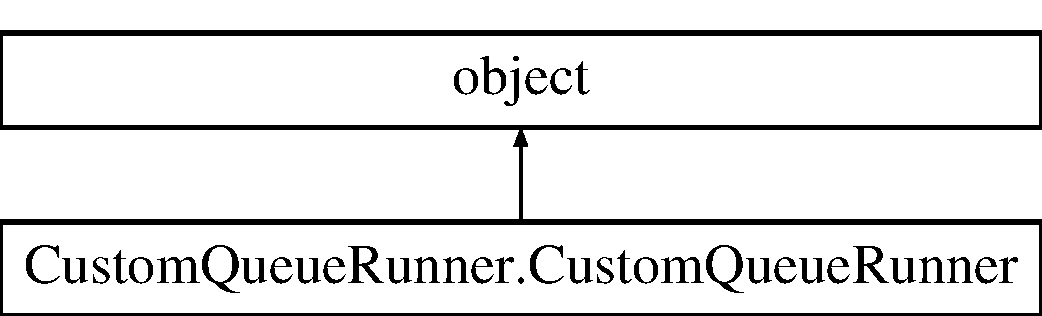
\includegraphics[height=2.000000cm]{classCustomQueueRunner_1_1CustomQueueRunner}
\end{center}
\end{figure}
\subsection*{Public Member Functions}
\begin{DoxyCompactItemize}
\item 
\hypertarget{classCustomQueueRunner_1_1CustomQueueRunner_af76d3fec912865bf7d94701af4e7c068}{def {\bfseries \-\_\-\-\_\-init\-\_\-\-\_\-}}\label{classCustomQueueRunner_1_1CustomQueueRunner_af76d3fec912865bf7d94701af4e7c068}

\item 
\hypertarget{classCustomQueueRunner_1_1CustomQueueRunner_a53f6b52ead2366c4c9982f7b0f76a8c9}{def {\bfseries file\-Name\-\_\-iterator}}\label{classCustomQueueRunner_1_1CustomQueueRunner_a53f6b52ead2366c4c9982f7b0f76a8c9}

\item 
\hypertarget{classCustomQueueRunner_1_1CustomQueueRunner_a597a93bdb86013eed4892c0722d3a313}{def {\bfseries thread\-\_\-read\-File}}\label{classCustomQueueRunner_1_1CustomQueueRunner_a597a93bdb86013eed4892c0722d3a313}

\item 
def \hyperlink{classCustomQueueRunner_1_1CustomQueueRunner_aa15d0ce6375f74387b8b85f28356bd8c}{data\-\_\-iterator}
\item 
def \hyperlink{classCustomQueueRunner_1_1CustomQueueRunner_a9146cfaf42a1bcd9b5511fb99a2c7115}{thread\-\_\-main}
\item 
def \hyperlink{classCustomQueueRunner_1_1CustomQueueRunner_ad43f2e2230cba3ee0e1162eafc763ccd}{start\-\_\-threads}
\end{DoxyCompactItemize}
\subsection*{Public Attributes}
\begin{DoxyCompactItemize}
\item 
\hypertarget{classCustomQueueRunner_1_1CustomQueueRunner_aa1b3c4a985bea0bd70b347ca7ad61b5a}{{\bfseries file\-Queue}}\label{classCustomQueueRunner_1_1CustomQueueRunner_aa1b3c4a985bea0bd70b347ca7ad61b5a}

\item 
\hypertarget{classCustomQueueRunner_1_1CustomQueueRunner_ab12ec1deb2c6373efdb06769bfb42bd5}{{\bfseries queue\-X}}\label{classCustomQueueRunner_1_1CustomQueueRunner_ab12ec1deb2c6373efdb06769bfb42bd5}

\item 
\hypertarget{classCustomQueueRunner_1_1CustomQueueRunner_af400c5ebfdcb41ba6d7e7404e75cd3ea}{{\bfseries data\-X}}\label{classCustomQueueRunner_1_1CustomQueueRunner_af400c5ebfdcb41ba6d7e7404e75cd3ea}

\item 
\hypertarget{classCustomQueueRunner_1_1CustomQueueRunner_a6105ffb054f8abcbd728f94cd44d543e}{{\bfseries data\-Y}}\label{classCustomQueueRunner_1_1CustomQueueRunner_a6105ffb054f8abcbd728f94cd44d543e}

\item 
\hypertarget{classCustomQueueRunner_1_1CustomQueueRunner_aee28109477b6419ffb41852410a99a9a}{{\bfseries data\-W}}\label{classCustomQueueRunner_1_1CustomQueueRunner_aee28109477b6419ffb41852410a99a9a}

\item 
\hypertarget{classCustomQueueRunner_1_1CustomQueueRunner_aa7bb789d918609955e2d755812855b33}{{\bfseries variables}}\label{classCustomQueueRunner_1_1CustomQueueRunner_aa7bb789d918609955e2d755812855b33}

\item 
\hypertarget{classCustomQueueRunner_1_1CustomQueueRunner_aed125859f24c11af006847d8c6613ca3}{{\bfseries batch\-\_\-size}}\label{classCustomQueueRunner_1_1CustomQueueRunner_aed125859f24c11af006847d8c6613ca3}

\item 
\hypertarget{classCustomQueueRunner_1_1CustomQueueRunner_a87afd27e4fba7b890ef7cf7056dd01be}{{\bfseries enqueue\-\_\-op\-X}}\label{classCustomQueueRunner_1_1CustomQueueRunner_a87afd27e4fba7b890ef7cf7056dd01be}

\item 
\hypertarget{classCustomQueueRunner_1_1CustomQueueRunner_aba53122c1cf237949531b1c016628c76}{{\bfseries pt\-Reweight}}\label{classCustomQueueRunner_1_1CustomQueueRunner_aba53122c1cf237949531b1c016628c76}

\end{DoxyCompactItemize}


\subsection{Detailed Description}
\begin{DoxyVerb}This class manages the background threads needed to fill
    a queue full of data.
\end{DoxyVerb}
 

\subsection{Member Function Documentation}
\hypertarget{classCustomQueueRunner_1_1CustomQueueRunner_aa15d0ce6375f74387b8b85f28356bd8c}{\index{Custom\-Queue\-Runner\-::\-Custom\-Queue\-Runner@{Custom\-Queue\-Runner\-::\-Custom\-Queue\-Runner}!data\-\_\-iterator@{data\-\_\-iterator}}
\index{data\-\_\-iterator@{data\-\_\-iterator}!CustomQueueRunner::CustomQueueRunner@{Custom\-Queue\-Runner\-::\-Custom\-Queue\-Runner}}
\subsubsection[{data\-\_\-iterator}]{\setlength{\rightskip}{0pt plus 5cm}def Custom\-Queue\-Runner.\-Custom\-Queue\-Runner.\-data\-\_\-iterator (
\begin{DoxyParamCaption}
\item[{}]{self}
\end{DoxyParamCaption}
)}}\label{classCustomQueueRunner_1_1CustomQueueRunner_aa15d0ce6375f74387b8b85f28356bd8c}
\begin{DoxyVerb}A simple data iterator \end{DoxyVerb}
 \hypertarget{classCustomQueueRunner_1_1CustomQueueRunner_ad43f2e2230cba3ee0e1162eafc763ccd}{\index{Custom\-Queue\-Runner\-::\-Custom\-Queue\-Runner@{Custom\-Queue\-Runner\-::\-Custom\-Queue\-Runner}!start\-\_\-threads@{start\-\_\-threads}}
\index{start\-\_\-threads@{start\-\_\-threads}!CustomQueueRunner::CustomQueueRunner@{Custom\-Queue\-Runner\-::\-Custom\-Queue\-Runner}}
\subsubsection[{start\-\_\-threads}]{\setlength{\rightskip}{0pt plus 5cm}def Custom\-Queue\-Runner.\-Custom\-Queue\-Runner.\-start\-\_\-threads (
\begin{DoxyParamCaption}
\item[{}]{self, }
\item[{}]{sess, }
\item[{}]{n\-\_\-threads = {\ttfamily 1}}
\end{DoxyParamCaption}
)}}\label{classCustomQueueRunner_1_1CustomQueueRunner_ad43f2e2230cba3ee0e1162eafc763ccd}
\begin{DoxyVerb}Start background threads to feed queue \end{DoxyVerb}
 \hypertarget{classCustomQueueRunner_1_1CustomQueueRunner_a9146cfaf42a1bcd9b5511fb99a2c7115}{\index{Custom\-Queue\-Runner\-::\-Custom\-Queue\-Runner@{Custom\-Queue\-Runner\-::\-Custom\-Queue\-Runner}!thread\-\_\-main@{thread\-\_\-main}}
\index{thread\-\_\-main@{thread\-\_\-main}!CustomQueueRunner::CustomQueueRunner@{Custom\-Queue\-Runner\-::\-Custom\-Queue\-Runner}}
\subsubsection[{thread\-\_\-main}]{\setlength{\rightskip}{0pt plus 5cm}def Custom\-Queue\-Runner.\-Custom\-Queue\-Runner.\-thread\-\_\-main (
\begin{DoxyParamCaption}
\item[{}]{self, }
\item[{}]{sess}
\end{DoxyParamCaption}
)}}\label{classCustomQueueRunner_1_1CustomQueueRunner_a9146cfaf42a1bcd9b5511fb99a2c7115}
\begin{DoxyVerb}Function run on alternate thread. Basically, keep adding data to the queue.
\end{DoxyVerb}
 

The documentation for this class was generated from the following file\-:\begin{DoxyCompactItemize}
\item 
/home/travis/build/susy2015/\-Top\-Tagger/\-Tools/python/Custom\-Queue\-Runner.\-py\end{DoxyCompactItemize}

\hypertarget{classDataGetter_1_1DataGetter}{\section{Data\-Getter.\-Data\-Getter Class Reference}
\label{classDataGetter_1_1DataGetter}\index{Data\-Getter.\-Data\-Getter@{Data\-Getter.\-Data\-Getter}}
}
\subsection*{Public Member Functions}
\begin{DoxyCompactItemize}
\item 
\hypertarget{classDataGetter_1_1DataGetter_a9b80011f43e1928b3cbcf53417add1c9}{def {\bfseries \-\_\-\-\_\-init\-\_\-\-\_\-}}\label{classDataGetter_1_1DataGetter_a9b80011f43e1928b3cbcf53417add1c9}

\item 
\hypertarget{classDataGetter_1_1DataGetter_a185354693ff9e0d0433f2c27591afbbf}{def {\bfseries Standard\-Variables}}\label{classDataGetter_1_1DataGetter_a185354693ff9e0d0433f2c27591afbbf}

\item 
\hypertarget{classDataGetter_1_1DataGetter_aeb839377e4bfab6da9c83ec70be291cd}{def {\bfseries Defined\-Variables}}\label{classDataGetter_1_1DataGetter_aeb839377e4bfab6da9c83ec70be291cd}

\item 
\hypertarget{classDataGetter_1_1DataGetter_af8c40c8e6ee7597e785d6e967d1b90c2}{def {\bfseries get\-List}}\label{classDataGetter_1_1DataGetter_af8c40c8e6ee7597e785d6e967d1b90c2}

\item 
\hypertarget{classDataGetter_1_1DataGetter_ab1c1ff5985bdd64e20eb6a1292c2afa5}{def {\bfseries prescale\-Background}}\label{classDataGetter_1_1DataGetter_ab1c1ff5985bdd64e20eb6a1292c2afa5}

\item 
\hypertarget{classDataGetter_1_1DataGetter_aa9320b82c24d8e5885881891c7e58dce}{def {\bfseries import\-Data}}\label{classDataGetter_1_1DataGetter_aa9320b82c24d8e5885881891c7e58dce}

\end{DoxyCompactItemize}
\subsection*{Public Attributes}
\begin{DoxyCompactItemize}
\item 
\hypertarget{classDataGetter_1_1DataGetter_a2739938ac344ad65b1d2e25e2c787419}{{\bfseries list}}\label{classDataGetter_1_1DataGetter_a2739938ac344ad65b1d2e25e2c787419}

\item 
\hypertarget{classDataGetter_1_1DataGetter_a9d4f5ce1a7aae31b19aa9171cb0b62ac}{{\bfseries buffer\-Data}}\label{classDataGetter_1_1DataGetter_a9d4f5ce1a7aae31b19aa9171cb0b62ac}

\item 
\hypertarget{classDataGetter_1_1DataGetter_ad47a039976844990578f9b9d5e2301c3}{{\bfseries data\-Map}}\label{classDataGetter_1_1DataGetter_ad47a039976844990578f9b9d5e2301c3}

\end{DoxyCompactItemize}


The documentation for this class was generated from the following file\-:\begin{DoxyCompactItemize}
\item 
/home/travis/build/susy2015/\-Top\-Tagger/\-Tools/python/Data\-Getter.\-py\end{DoxyCompactItemize}

\hypertarget{classDataManager_1_1DataManager}{\section{Data\-Manager.\-Data\-Manager Class Reference}
\label{classDataManager_1_1DataManager}\index{Data\-Manager.\-Data\-Manager@{Data\-Manager.\-Data\-Manager}}
}
\subsection*{Public Member Functions}
\begin{DoxyCompactItemize}
\item 
\hypertarget{classDataManager_1_1DataManager_a6720284570316a8b502e468074e22d28}{def {\bfseries \-\_\-\-\_\-init\-\_\-\-\_\-}}\label{classDataManager_1_1DataManager_a6720284570316a8b502e468074e22d28}

\item 
\hypertarget{classDataManager_1_1DataManager_adfc56295e24739346eb4673877ae0277}{def {\bfseries start\-File\-Queues}}\label{classDataManager_1_1DataManager_adfc56295e24739346eb4673877ae0277}

\item 
\hypertarget{classDataManager_1_1DataManager_a8dc65af6fee5bd5bb20f0191848fa2fb}{def {\bfseries start\-Data\-Queues}}\label{classDataManager_1_1DataManager_a8dc65af6fee5bd5bb20f0191848fa2fb}

\item 
\hypertarget{classDataManager_1_1DataManager_adc8376ebbcc8fd94f8e7cc2b5ab2e16d}{def {\bfseries launch\-Queue\-Threads}}\label{classDataManager_1_1DataManager_adc8376ebbcc8fd94f8e7cc2b5ab2e16d}

\item 
\hypertarget{classDataManager_1_1DataManager_a7c93e51eb6673ea46f7fb694b65136c3}{def {\bfseries continue\-Training\-Loop}}\label{classDataManager_1_1DataManager_a7c93e51eb6673ea46f7fb694b65136c3}

\item 
\hypertarget{classDataManager_1_1DataManager_ab05ed3527245d208513637a4985415cd}{def {\bfseries continue\-Flushing\-Queue}}\label{classDataManager_1_1DataManager_ab05ed3527245d208513637a4985415cd}

\item 
\hypertarget{classDataManager_1_1DataManager_a2b48ff573d4ebab478b2e27190a5d069}{def {\bfseries request\-Stop}}\label{classDataManager_1_1DataManager_a2b48ff573d4ebab478b2e27190a5d069}

\item 
\hypertarget{classDataManager_1_1DataManager_a43c7d931d591e95fd4d8572d008dd5e6}{def {\bfseries join}}\label{classDataManager_1_1DataManager_a43c7d931d591e95fd4d8572d008dd5e6}

\end{DoxyCompactItemize}
\subsection*{Public Attributes}
\begin{DoxyCompactItemize}
\item 
\hypertarget{classDataManager_1_1DataManager_a601a92a29ce1628428bfac190af9c5cf}{{\bfseries n\-Epoch}}\label{classDataManager_1_1DataManager_a601a92a29ce1628428bfac190af9c5cf}

\item 
\hypertarget{classDataManager_1_1DataManager_ac7399c255de1bf5d153359e031742ddf}{{\bfseries input\-Data\-Queue}}\label{classDataManager_1_1DataManager_ac7399c255de1bf5d153359e031742ddf}

\item 
\hypertarget{classDataManager_1_1DataManager_a3ae70618c6582c9ed2c8d7f9f7eea5c6}{{\bfseries sig\-Scale\-Sum}}\label{classDataManager_1_1DataManager_a3ae70618c6582c9ed2c8d7f9f7eea5c6}

\item 
\hypertarget{classDataManager_1_1DataManager_aa384d054b72b38547f1784921dd28d2f}{{\bfseries sig\-Data\-Samples}}\label{classDataManager_1_1DataManager_aa384d054b72b38547f1784921dd28d2f}

\item 
\hypertarget{classDataManager_1_1DataManager_a0a1506a6aa38f28efc2a423fb1e4d82c}{{\bfseries bg\-Scale\-Sum}}\label{classDataManager_1_1DataManager_a0a1506a6aa38f28efc2a423fb1e4d82c}

\item 
\hypertarget{classDataManager_1_1DataManager_afaac724759cf44f46d0ed4214384f549}{{\bfseries bg\-Data\-Samples}}\label{classDataManager_1_1DataManager_afaac724759cf44f46d0ed4214384f549}

\item 
\hypertarget{classDataManager_1_1DataManager_a3286c308c0ff5f86f91126838273088f}{{\bfseries coord\-S1}}\label{classDataManager_1_1DataManager_a3286c308c0ff5f86f91126838273088f}

\item 
\hypertarget{classDataManager_1_1DataManager_a33d474a8010c2235c48cd10407b0f9e2}{{\bfseries coord\-S2}}\label{classDataManager_1_1DataManager_a33d474a8010c2235c48cd10407b0f9e2}

\item 
\hypertarget{classDataManager_1_1DataManager_a0da4da348d64b2764ec2a79e3d6e0c50}{{\bfseries threads\-S2}}\label{classDataManager_1_1DataManager_a0da4da348d64b2764ec2a79e3d6e0c50}

\item 
\hypertarget{classDataManager_1_1DataManager_af320ecb779efb8f5d91a13893f5c23b7}{{\bfseries qr}}\label{classDataManager_1_1DataManager_af320ecb779efb8f5d91a13893f5c23b7}

\item 
\hypertarget{classDataManager_1_1DataManager_acb651b61c2cc6cc2cae36eda745cc2c4}{{\bfseries threads\-S1}}\label{classDataManager_1_1DataManager_acb651b61c2cc6cc2cae36eda745cc2c4}

\end{DoxyCompactItemize}


The documentation for this class was generated from the following file\-:\begin{DoxyCompactItemize}
\item 
/home/travis/build/susy2015/\-Top\-Tagger/\-Tools/python/Data\-Manager.\-py\end{DoxyCompactItemize}

\hypertarget{classDataSample_1_1DataSample}{\section{Data\-Sample.\-Data\-Sample Class Reference}
\label{classDataSample_1_1DataSample}\index{Data\-Sample.\-Data\-Sample@{Data\-Sample.\-Data\-Sample}}
}
\subsection*{Public Member Functions}
\begin{DoxyCompactItemize}
\item 
\hypertarget{classDataSample_1_1DataSample_a94ba878e73df4d60f17581f71576f03c}{def {\bfseries \-\_\-\-\_\-init\-\_\-\-\_\-}}\label{classDataSample_1_1DataSample_a94ba878e73df4d60f17581f71576f03c}

\item 
\hypertarget{classDataSample_1_1DataSample_a21d87e9f6905da42dbddebbed7ad8cc7}{def {\bfseries start\-\_\-threads}}\label{classDataSample_1_1DataSample_a21d87e9f6905da42dbddebbed7ad8cc7}

\item 
\hypertarget{classDataSample_1_1DataSample_ad6f67ff2e39757b15a56491b439705e4}{def {\bfseries get\-Enqueue\-Op}}\label{classDataSample_1_1DataSample_ad6f67ff2e39757b15a56491b439705e4}

\end{DoxyCompactItemize}
\subsection*{Public Attributes}
\begin{DoxyCompactItemize}
\item 
\hypertarget{classDataSample_1_1DataSample_afb978dd6a2f37f5c485c54e0522c519a}{{\bfseries data\-Set}}\label{classDataSample_1_1DataSample_afb978dd6a2f37f5c485c54e0522c519a}

\item 
\hypertarget{classDataSample_1_1DataSample_a7da3ab30da6f0a9798aba2741c989ba8}{{\bfseries input\-Data\-Queue}}\label{classDataSample_1_1DataSample_a7da3ab30da6f0a9798aba2741c989ba8}

\item 
\hypertarget{classDataSample_1_1DataSample_acb8e500209d8092ebec32e630d8ee98a}{{\bfseries queue}}\label{classDataSample_1_1DataSample_acb8e500209d8092ebec32e630d8ee98a}

\item 
\hypertarget{classDataSample_1_1DataSample_a1edf25a363d46700d35180dbc19a0d70}{{\bfseries scale\-Factor}}\label{classDataSample_1_1DataSample_a1edf25a363d46700d35180dbc19a0d70}

\item 
\hypertarget{classDataSample_1_1DataSample_a0053c8db256081a6f6a87c6113e5997d}{{\bfseries batch\-Size}}\label{classDataSample_1_1DataSample_a0053c8db256081a6f6a87c6113e5997d}

\item 
\hypertarget{classDataSample_1_1DataSample_a1dc78865330341b82476c9718e0b2aae}{{\bfseries file\-List}}\label{classDataSample_1_1DataSample_a1dc78865330341b82476c9718e0b2aae}

\item 
\hypertarget{classDataSample_1_1DataSample_a130d097d0226e267d775230b858c56b3}{{\bfseries file\-Queue}}\label{classDataSample_1_1DataSample_a130d097d0226e267d775230b858c56b3}

\item 
\hypertarget{classDataSample_1_1DataSample_a61077c185f07df04d8df3b81439235fd}{{\bfseries custom\-Runner}}\label{classDataSample_1_1DataSample_a61077c185f07df04d8df3b81439235fd}

\end{DoxyCompactItemize}


The documentation for this class was generated from the following file\-:\begin{DoxyCompactItemize}
\item 
/home/travis/build/susy2015/\-Top\-Tagger/\-Tools/python/Data\-Sample.\-py\end{DoxyCompactItemize}

\hypertarget{classDataSet_1_1DataSet}{\section{Data\-Set.\-Data\-Set Class Reference}
\label{classDataSet_1_1DataSet}\index{Data\-Set.\-Data\-Set@{Data\-Set.\-Data\-Set}}
}
\subsection*{Public Member Functions}
\begin{DoxyCompactItemize}
\item 
\hypertarget{classDataSet_1_1DataSet_ae3eb8140a6a2ff62586c52158cb4cf21}{def {\bfseries \-\_\-\-\_\-init\-\_\-\-\_\-}}\label{classDataSet_1_1DataSet_ae3eb8140a6a2ff62586c52158cb4cf21}

\end{DoxyCompactItemize}
\subsection*{Public Attributes}
\begin{DoxyCompactItemize}
\item 
\hypertarget{classDataSet_1_1DataSet_a31312e7ebc75a63846784ead3f5cf8d1}{{\bfseries file\-Glob}}\label{classDataSet_1_1DataSet_a31312e7ebc75a63846784ead3f5cf8d1}

\item 
\hypertarget{classDataSet_1_1DataSet_ada08c6b544a58467403e9ab421057b5f}{{\bfseries xsec}}\label{classDataSet_1_1DataSet_ada08c6b544a58467403e9ab421057b5f}

\item 
\hypertarget{classDataSet_1_1DataSet_a69beaca98bb3ebb6061af614c70c5a80}{{\bfseries Nevts}}\label{classDataSet_1_1DataSet_a69beaca98bb3ebb6061af614c70c5a80}

\item 
\hypertarget{classDataSet_1_1DataSet_a6813ebb37a959a59becf21a06fda7e1f}{{\bfseries k\-Factor}}\label{classDataSet_1_1DataSet_a6813ebb37a959a59becf21a06fda7e1f}

\item 
\hypertarget{classDataSet_1_1DataSet_aadcca5cbd9d7962486695097ea39f34b}{{\bfseries sig}}\label{classDataSet_1_1DataSet_aadcca5cbd9d7962486695097ea39f34b}

\item 
\hypertarget{classDataSet_1_1DataSet_a10068706fbc43da752a9a839cdedff1a}{{\bfseries domain}}\label{classDataSet_1_1DataSet_a10068706fbc43da752a9a839cdedff1a}

\item 
\hypertarget{classDataSet_1_1DataSet_a483dac2804e4ea9d834d944ba9d5664e}{{\bfseries prescale}}\label{classDataSet_1_1DataSet_a483dac2804e4ea9d834d944ba9d5664e}

\item 
\hypertarget{classDataSet_1_1DataSet_ac5ea1a521dbffb539f7ccce804b64393}{{\bfseries rescale}}\label{classDataSet_1_1DataSet_ac5ea1a521dbffb539f7ccce804b64393}

\item 
\hypertarget{classDataSet_1_1DataSet_a290520ed790c13b0b0eb84a3530f9167}{{\bfseries n\-Enqueue\-Threads}}\label{classDataSet_1_1DataSet_a290520ed790c13b0b0eb84a3530f9167}

\item 
\hypertarget{classDataSet_1_1DataSet_afc8436a9d89b2ac89ca52552827303c3}{{\bfseries weight\-Hist}}\label{classDataSet_1_1DataSet_afc8436a9d89b2ac89ca52552827303c3}

\end{DoxyCompactItemize}


The documentation for this class was generated from the following file\-:\begin{DoxyCompactItemize}
\item 
/home/travis/build/susy2015/\-Top\-Tagger/\-Tools/python/Data\-Set.\-py\end{DoxyCompactItemize}

\hypertarget{structhcalcfg_1_1ParserDestroyExistsRecognizer_1_1DestroyExistsType}{\section{hcalcfg\-:\-:Parser\-Destroy\-Exists\-Recognizer$<$ T $>$\-:\-:Destroy\-Exists\-Type Struct Reference}
\label{structhcalcfg_1_1ParserDestroyExistsRecognizer_1_1DestroyExistsType}\index{hcalcfg\-::\-Parser\-Destroy\-Exists\-Recognizer$<$ T $>$\-::\-Destroy\-Exists\-Type@{hcalcfg\-::\-Parser\-Destroy\-Exists\-Recognizer$<$ T $>$\-::\-Destroy\-Exists\-Type}}
}
\subsection*{Public Attributes}
\begin{DoxyCompactItemize}
\item 
\hypertarget{structhcalcfg_1_1ParserDestroyExistsRecognizer_1_1DestroyExistsType_a58e21309aaeea19a0304b575ff8a566f}{char {\bfseries dummy1}}\label{structhcalcfg_1_1ParserDestroyExistsRecognizer_1_1DestroyExistsType_a58e21309aaeea19a0304b575ff8a566f}

\item 
\hypertarget{structhcalcfg_1_1ParserDestroyExistsRecognizer_1_1DestroyExistsType_a556b05d88dc0b53431250e59b76ca542}{char {\bfseries dummy2}}\label{structhcalcfg_1_1ParserDestroyExistsRecognizer_1_1DestroyExistsType_a556b05d88dc0b53431250e59b76ca542}

\end{DoxyCompactItemize}


The documentation for this struct was generated from the following file\-:\begin{DoxyCompactItemize}
\item 
/home/travis/build/susy2015/\-Top\-Tagger/\-Cfg\-Parser/src/Parser.\-cpp\end{DoxyCompactItemize}

\hypertarget{structhcalcfg_1_1ParserDestroyExistsRecognizer_1_1DestroyIsMissingType}{\section{hcalcfg\-:\-:Parser\-Destroy\-Exists\-Recognizer$<$ T $>$\-:\-:Destroy\-Is\-Missing\-Type Struct Reference}
\label{structhcalcfg_1_1ParserDestroyExistsRecognizer_1_1DestroyIsMissingType}\index{hcalcfg\-::\-Parser\-Destroy\-Exists\-Recognizer$<$ T $>$\-::\-Destroy\-Is\-Missing\-Type@{hcalcfg\-::\-Parser\-Destroy\-Exists\-Recognizer$<$ T $>$\-::\-Destroy\-Is\-Missing\-Type}}
}
\subsection*{Public Attributes}
\begin{DoxyCompactItemize}
\item 
\hypertarget{structhcalcfg_1_1ParserDestroyExistsRecognizer_1_1DestroyIsMissingType_a348be875a5ce8f5fd270f5d94a472e1f}{char {\bfseries dummy1}}\label{structhcalcfg_1_1ParserDestroyExistsRecognizer_1_1DestroyIsMissingType_a348be875a5ce8f5fd270f5d94a472e1f}

\end{DoxyCompactItemize}


The documentation for this struct was generated from the following file\-:\begin{DoxyCompactItemize}
\item 
/home/travis/build/susy2015/\-Top\-Tagger/\-Cfg\-Parser/src/Parser.\-cpp\end{DoxyCompactItemize}

\hypertarget{structLester_1_1EllipseParams}{\section{Lester\-:\-:Ellipse\-Params Struct Reference}
\label{structLester_1_1EllipseParams}\index{Lester\-::\-Ellipse\-Params@{Lester\-::\-Ellipse\-Params}}
}
\subsection*{Public Member Functions}
\begin{DoxyCompactItemize}
\item 
\hypertarget{structLester_1_1EllipseParams_a38ae9677eb46aee9fcd5aa51c86ae9a8}{{\bfseries Ellipse\-Params} (const double c\-\_\-xx2, const double c\-\_\-yy2, const double c\-\_\-xy2, const double c\-\_\-x2, const double c\-\_\-y2, const double c2)}\label{structLester_1_1EllipseParams_a38ae9677eb46aee9fcd5aa51c86ae9a8}

\item 
\hypertarget{structLester_1_1EllipseParams_ad4cc8073619a8224ece6e6bed8d3ccd2}{void {\bfseries set\-Det} ()}\label{structLester_1_1EllipseParams_ad4cc8073619a8224ece6e6bed8d3ccd2}

\item 
\hypertarget{structLester_1_1EllipseParams_a74def2b1875f0381b692341826503035}{{\bfseries Ellipse\-Params} (const double x0, const double y0)}\label{structLester_1_1EllipseParams_a74def2b1875f0381b692341826503035}

\item 
\hypertarget{structLester_1_1EllipseParams_a9b99b405ad6f4635e9d726ad4b70fb1d}{double {\bfseries lester\-Factor} (const \hyperlink{structLester_1_1EllipseParams}{Ellipse\-Params} \&e2) const }\label{structLester_1_1EllipseParams_a9b99b405ad6f4635e9d726ad4b70fb1d}

\item 
\hypertarget{structLester_1_1EllipseParams_af0428a20e24e380a4abebc7b201afcc0}{bool {\bfseries operator==} (const \hyperlink{structLester_1_1EllipseParams}{Ellipse\-Params} \&other) const }\label{structLester_1_1EllipseParams_af0428a20e24e380a4abebc7b201afcc0}

\end{DoxyCompactItemize}
\subsection*{Public Attributes}
\begin{DoxyCompactItemize}
\item 
\hypertarget{structLester_1_1EllipseParams_a95afe64aa1687111e1317fa4045fc55c}{double {\bfseries c\-\_\-xx}}\label{structLester_1_1EllipseParams_a95afe64aa1687111e1317fa4045fc55c}

\item 
\hypertarget{structLester_1_1EllipseParams_a494ff14d11c07b4428bca666ea8343b3}{double {\bfseries c\-\_\-yy}}\label{structLester_1_1EllipseParams_a494ff14d11c07b4428bca666ea8343b3}

\item 
\hypertarget{structLester_1_1EllipseParams_a4f0a5a453728e503760325677c01b713}{double {\bfseries c\-\_\-xy}}\label{structLester_1_1EllipseParams_a4f0a5a453728e503760325677c01b713}

\item 
\hypertarget{structLester_1_1EllipseParams_a6c0631a050a6564c804c35aea4997c29}{double {\bfseries c\-\_\-x}}\label{structLester_1_1EllipseParams_a6c0631a050a6564c804c35aea4997c29}

\item 
\hypertarget{structLester_1_1EllipseParams_a8b000ff58e2ff2511da0f6234e191e6e}{double {\bfseries c\-\_\-y}}\label{structLester_1_1EllipseParams_a8b000ff58e2ff2511da0f6234e191e6e}

\item 
\hypertarget{structLester_1_1EllipseParams_a86dd4c4bad1eee26d81071efa1137114}{double {\bfseries c}}\label{structLester_1_1EllipseParams_a86dd4c4bad1eee26d81071efa1137114}

\item 
\hypertarget{structLester_1_1EllipseParams_ad777140c2b6da121e1fa322b76b12a9e}{double {\bfseries det}}\label{structLester_1_1EllipseParams_ad777140c2b6da121e1fa322b76b12a9e}

\end{DoxyCompactItemize}


The documentation for this struct was generated from the following file\-:\begin{DoxyCompactItemize}
\item 
/home/travis/build/susy2015/\-Top\-Tagger/\-Top\-Tagger/interface/lester\-\_\-mt2\-\_\-bisect.\-h\end{DoxyCompactItemize}

\hypertarget{classhcalcfg_1_1Errors}{\section{hcalcfg\-:\-:Errors Class Reference}
\label{classhcalcfg_1_1Errors}\index{hcalcfg\-::\-Errors@{hcalcfg\-::\-Errors}}
}
\subsection*{Public Member Functions}
\begin{DoxyCompactItemize}
\item 
\hypertarget{classhcalcfg_1_1Errors_aadf51ffffaf63b6631be27497cef691e}{void {\bfseries Syn\-Err} (int line, int col, int n)}\label{classhcalcfg_1_1Errors_aadf51ffffaf63b6631be27497cef691e}

\item 
\hypertarget{classhcalcfg_1_1Errors_a7ec37002c80b092716799a1b83b77f4c}{void {\bfseries Error} (int line, int col, const wchar\-\_\-t $\ast$s)}\label{classhcalcfg_1_1Errors_a7ec37002c80b092716799a1b83b77f4c}

\item 
\hypertarget{classhcalcfg_1_1Errors_a8782ed816d70b9455df23f9b0b7d9f1c}{void {\bfseries Warning} (int line, int col, const wchar\-\_\-t $\ast$s)}\label{classhcalcfg_1_1Errors_a8782ed816d70b9455df23f9b0b7d9f1c}

\item 
\hypertarget{classhcalcfg_1_1Errors_a0de033b0829bbd7b0e53f92249dde549}{void {\bfseries Warning} (const wchar\-\_\-t $\ast$s)}\label{classhcalcfg_1_1Errors_a0de033b0829bbd7b0e53f92249dde549}

\item 
\hypertarget{classhcalcfg_1_1Errors_a9b4437d7f820fe03d1a7ae84a20830d7}{void {\bfseries Exception} (const wchar\-\_\-t $\ast$s)}\label{classhcalcfg_1_1Errors_a9b4437d7f820fe03d1a7ae84a20830d7}

\end{DoxyCompactItemize}
\subsection*{Public Attributes}
\begin{DoxyCompactItemize}
\item 
\hypertarget{classhcalcfg_1_1Errors_aa493a10b51d31629b0224656871320ee}{int {\bfseries count}}\label{classhcalcfg_1_1Errors_aa493a10b51d31629b0224656871320ee}

\end{DoxyCompactItemize}


The documentation for this class was generated from the following files\-:\begin{DoxyCompactItemize}
\item 
/home/travis/build/susy2015/\-Top\-Tagger/\-Cfg\-Parser/include/Parser.\-h\item 
/home/travis/build/susy2015/\-Top\-Tagger/\-Cfg\-Parser/src/Parser.\-cpp\end{DoxyCompactItemize}

\hypertarget{structhcalcfg_1_1ParserDestroyExistsRecognizer_1_1ExistsIfDestroyIsDefinedMarker}{\section{hcalcfg\-:\-:Parser\-Destroy\-Exists\-Recognizer$<$ T $>$\-:\-:Exists\-If\-Destroy\-Is\-Defined\-Marker$<$ U, $>$ Struct Template Reference}
\label{structhcalcfg_1_1ParserDestroyExistsRecognizer_1_1ExistsIfDestroyIsDefinedMarker}\index{hcalcfg\-::\-Parser\-Destroy\-Exists\-Recognizer$<$ T $>$\-::\-Exists\-If\-Destroy\-Is\-Defined\-Marker$<$ U, $>$@{hcalcfg\-::\-Parser\-Destroy\-Exists\-Recognizer$<$ T $>$\-::\-Exists\-If\-Destroy\-Is\-Defined\-Marker$<$ U, $>$}}
}


The documentation for this struct was generated from the following file\-:\begin{DoxyCompactItemize}
\item 
/home/travis/build/susy2015/\-Top\-Tagger/\-Cfg\-Parser/src/Parser.\-cpp\end{DoxyCompactItemize}

\hypertarget{structhcalcfg_1_1ParserInitExistsRecognizer_1_1ExistsIfInitIsDefinedMarker}{\section{hcalcfg\-:\-:Parser\-Init\-Exists\-Recognizer$<$ T $>$\-:\-:Exists\-If\-Init\-Is\-Defined\-Marker$<$ U, $>$ Struct Template Reference}
\label{structhcalcfg_1_1ParserInitExistsRecognizer_1_1ExistsIfInitIsDefinedMarker}\index{hcalcfg\-::\-Parser\-Init\-Exists\-Recognizer$<$ T $>$\-::\-Exists\-If\-Init\-Is\-Defined\-Marker$<$ U, $>$@{hcalcfg\-::\-Parser\-Init\-Exists\-Recognizer$<$ T $>$\-::\-Exists\-If\-Init\-Is\-Defined\-Marker$<$ U, $>$}}
}


The documentation for this struct was generated from the following file\-:\begin{DoxyCompactItemize}
\item 
/home/travis/build/susy2015/\-Top\-Tagger/\-Cfg\-Parser/src/Parser.\-cpp\end{DoxyCompactItemize}

\hypertarget{classFileNameQueue_1_1FileNameQueue}{\section{File\-Name\-Queue.\-File\-Name\-Queue Class Reference}
\label{classFileNameQueue_1_1FileNameQueue}\index{File\-Name\-Queue.\-File\-Name\-Queue@{File\-Name\-Queue.\-File\-Name\-Queue}}
}
\subsection*{Public Member Functions}
\begin{DoxyCompactItemize}
\item 
\hypertarget{classFileNameQueue_1_1FileNameQueue_aea39c38145599ec2d9bec31ac8cef68a}{def {\bfseries \-\_\-\-\_\-init\-\_\-\-\_\-}}\label{classFileNameQueue_1_1FileNameQueue_aea39c38145599ec2d9bec31ac8cef68a}

\item 
\hypertarget{classFileNameQueue_1_1FileNameQueue_abaed28219f3e10239097d7874472678d}{def {\bfseries add\-Custom\-Runner\-Threads}}\label{classFileNameQueue_1_1FileNameQueue_abaed28219f3e10239097d7874472678d}

\item 
\hypertarget{classFileNameQueue_1_1FileNameQueue_a91c5b679677cc9664dd2c16822d042e1}{def {\bfseries get\-Queue}}\label{classFileNameQueue_1_1FileNameQueue_a91c5b679677cc9664dd2c16822d042e1}

\item 
\hypertarget{classFileNameQueue_1_1FileNameQueue_aa0fad18a33d8a60e45fb56b808011667}{def {\bfseries get}}\label{classFileNameQueue_1_1FileNameQueue_aa0fad18a33d8a60e45fb56b808011667}

\item 
\hypertarget{classFileNameQueue_1_1FileNameQueue_af9c7379a4367c2ca928c7a63266e5ff5}{def {\bfseries queue\-Process}}\label{classFileNameQueue_1_1FileNameQueue_af9c7379a4367c2ca928c7a63266e5ff5}

\item 
\hypertarget{classFileNameQueue_1_1FileNameQueue_a3655c497dd707c8681369cd70b4272c3}{def {\bfseries start\-Queue\-Process}}\label{classFileNameQueue_1_1FileNameQueue_a3655c497dd707c8681369cd70b4272c3}

\end{DoxyCompactItemize}
\subsection*{Public Attributes}
\begin{DoxyCompactItemize}
\item 
\hypertarget{classFileNameQueue_1_1FileNameQueue_a7ab700eeebb00f7b586ff3ca7299b016}{{\bfseries files}}\label{classFileNameQueue_1_1FileNameQueue_a7ab700eeebb00f7b586ff3ca7299b016}

\item 
\hypertarget{classFileNameQueue_1_1FileNameQueue_ad4cac71c6ecb2d22c2e00b1b80cafd0c}{{\bfseries n\-Epoch}}\label{classFileNameQueue_1_1FileNameQueue_ad4cac71c6ecb2d22c2e00b1b80cafd0c}

\item 
\hypertarget{classFileNameQueue_1_1FileNameQueue_af94c59d51930e68104548a831501f746}{{\bfseries file\-Queue}}\label{classFileNameQueue_1_1FileNameQueue_af94c59d51930e68104548a831501f746}

\item 
\hypertarget{classFileNameQueue_1_1FileNameQueue_ab5d275ac643e94fdcffe97f1f8ab04d8}{{\bfseries input\-Data\-Queue}}\label{classFileNameQueue_1_1FileNameQueue_ab5d275ac643e94fdcffe97f1f8ab04d8}

\item 
\hypertarget{classFileNameQueue_1_1FileNameQueue_a95d463f60468ef0af146f969bdbf5c93}{{\bfseries custom\-Runner\-Threads}}\label{classFileNameQueue_1_1FileNameQueue_a95d463f60468ef0af146f969bdbf5c93}

\end{DoxyCompactItemize}


The documentation for this class was generated from the following file\-:\begin{DoxyCompactItemize}
\item 
/home/travis/build/susy2015/\-Top\-Tagger/\-Tools/python/File\-Name\-Queue.\-py\end{DoxyCompactItemize}

\hypertarget{classHDF5Writer}{\section{H\-D\-F5\-Writer Class Reference}
\label{classHDF5Writer}\index{H\-D\-F5\-Writer@{H\-D\-F5\-Writer}}
}
\subsection*{Public Member Functions}
\begin{DoxyCompactItemize}
\item 
\hypertarget{classHDF5Writer_ad8e416d1f0a705baf7af1307df1bd095}{{\bfseries H\-D\-F5\-Writer} (const std\-::map$<$ std\-::string, std\-::vector$<$ std\-::string $>$$>$ \&variables, int events\-Per\-File, const std\-::string \&ofname)}\label{classHDF5Writer_ad8e416d1f0a705baf7af1307df1bd095}

\item 
\hypertarget{classHDF5Writer_a636afc5a3f1d26c84eec5975e200418d}{void {\bfseries set\-Tuple\-Vars} (const std\-::set$<$ std\-::string $>$ \&)}\label{classHDF5Writer_a636afc5a3f1d26c84eec5975e200418d}

\item 
\hypertarget{classHDF5Writer_af0e59c14065285d91bc8e5dad4bfd7f9}{void {\bfseries init\-Branches} (const N\-Tuple\-Reader \&tr)}\label{classHDF5Writer_af0e59c14065285d91bc8e5dad4bfd7f9}

\item 
\hypertarget{classHDF5Writer_adbd14eba2d2d401d635ba6cbce691afe}{void {\bfseries save\-H\-D\-F5\-File} ()}\label{classHDF5Writer_adbd14eba2d2d401d635ba6cbce691afe}

\item 
\hypertarget{classHDF5Writer_af88c6deb22f565aa60a27dc5476a59e7}{void {\bfseries fill} ()}\label{classHDF5Writer_af88c6deb22f565aa60a27dc5476a59e7}

\end{DoxyCompactItemize}


The documentation for this class was generated from the following file\-:\begin{DoxyCompactItemize}
\item 
/home/travis/build/susy2015/\-Top\-Tagger/\-Tools/cpp/make\-Training\-Tuples.\-C\end{DoxyCompactItemize}

\hypertarget{structhcalcfg_1_1ParserInitExistsRecognizer_1_1InitExistsType}{\section{hcalcfg\-:\-:Parser\-Init\-Exists\-Recognizer$<$ T $>$\-:\-:Init\-Exists\-Type Struct Reference}
\label{structhcalcfg_1_1ParserInitExistsRecognizer_1_1InitExistsType}\index{hcalcfg\-::\-Parser\-Init\-Exists\-Recognizer$<$ T $>$\-::\-Init\-Exists\-Type@{hcalcfg\-::\-Parser\-Init\-Exists\-Recognizer$<$ T $>$\-::\-Init\-Exists\-Type}}
}
\subsection*{Public Attributes}
\begin{DoxyCompactItemize}
\item 
\hypertarget{structhcalcfg_1_1ParserInitExistsRecognizer_1_1InitExistsType_a2fc61d9af56981864327d3338dda7026}{char {\bfseries dummy1}}\label{structhcalcfg_1_1ParserInitExistsRecognizer_1_1InitExistsType_a2fc61d9af56981864327d3338dda7026}

\item 
\hypertarget{structhcalcfg_1_1ParserInitExistsRecognizer_1_1InitExistsType_ae89b7adefe99bc3fa6708783213f8c47}{char {\bfseries dummy2}}\label{structhcalcfg_1_1ParserInitExistsRecognizer_1_1InitExistsType_ae89b7adefe99bc3fa6708783213f8c47}

\end{DoxyCompactItemize}


The documentation for this struct was generated from the following file\-:\begin{DoxyCompactItemize}
\item 
/home/travis/build/susy2015/\-Top\-Tagger/\-Cfg\-Parser/src/Parser.\-cpp\end{DoxyCompactItemize}

\hypertarget{structhcalcfg_1_1ParserInitExistsRecognizer_1_1InitIsMissingType}{\section{hcalcfg\-:\-:Parser\-Init\-Exists\-Recognizer$<$ T $>$\-:\-:Init\-Is\-Missing\-Type Struct Reference}
\label{structhcalcfg_1_1ParserInitExistsRecognizer_1_1InitIsMissingType}\index{hcalcfg\-::\-Parser\-Init\-Exists\-Recognizer$<$ T $>$\-::\-Init\-Is\-Missing\-Type@{hcalcfg\-::\-Parser\-Init\-Exists\-Recognizer$<$ T $>$\-::\-Init\-Is\-Missing\-Type}}
}
\subsection*{Public Attributes}
\begin{DoxyCompactItemize}
\item 
\hypertarget{structhcalcfg_1_1ParserInitExistsRecognizer_1_1InitIsMissingType_abb1ead880d0054dbf127306fcc9804ac}{char {\bfseries dummy1}}\label{structhcalcfg_1_1ParserInitExistsRecognizer_1_1InitIsMissingType_abb1ead880d0054dbf127306fcc9804ac}

\end{DoxyCompactItemize}


The documentation for this struct was generated from the following file\-:\begin{DoxyCompactItemize}
\item 
/home/travis/build/susy2015/\-Top\-Tagger/\-Cfg\-Parser/src/Parser.\-cpp\end{DoxyCompactItemize}

\hypertarget{classhcalcfg_1_1KeywordMap}{\section{hcalcfg\-:\-:Keyword\-Map Class Reference}
\label{classhcalcfg_1_1KeywordMap}\index{hcalcfg\-::\-Keyword\-Map@{hcalcfg\-::\-Keyword\-Map}}
}
\subsection*{Public Member Functions}
\begin{DoxyCompactItemize}
\item 
\hypertarget{classhcalcfg_1_1KeywordMap_aa4ea52d85eb56ee4eb463014618dabc1}{void {\bfseries set} (const wchar\-\_\-t $\ast$key, int val)}\label{classhcalcfg_1_1KeywordMap_aa4ea52d85eb56ee4eb463014618dabc1}

\item 
\hypertarget{classhcalcfg_1_1KeywordMap_a964e6f3248099709f52c76b3f4c049f4}{int {\bfseries get} (const wchar\-\_\-t $\ast$key, int default\-Val)}\label{classhcalcfg_1_1KeywordMap_a964e6f3248099709f52c76b3f4c049f4}

\end{DoxyCompactItemize}


The documentation for this class was generated from the following file\-:\begin{DoxyCompactItemize}
\item 
/home/travis/build/susy2015/\-Top\-Tagger/\-Cfg\-Parser/include/Scanner.\-h\end{DoxyCompactItemize}

\hypertarget{classcfg_1_1Literal}{\section{cfg\-:\-:Literal Class Reference}
\label{classcfg_1_1Literal}\index{cfg\-::\-Literal@{cfg\-::\-Literal}}
}
\subsection*{Public Types}
\begin{DoxyCompactItemize}
\item 
enum {\bfseries Flavor} \{ \\*
{\bfseries fl\-\_\-\-Null}, 
{\bfseries fl\-\_\-\-String}, 
{\bfseries fl\-\_\-\-Boolean}, 
{\bfseries fl\-\_\-\-Integer}, 
\\*
{\bfseries fl\-\_\-\-Float}
 \}
\end{DoxyCompactItemize}
\subsection*{Public Member Functions}
\begin{DoxyCompactItemize}
\item 
\hypertarget{classcfg_1_1Literal_aa7cad9d482f1d3e3305ebf2b9c6f7fb8}{{\bfseries Literal} (const std\-::string \&val)}\label{classcfg_1_1Literal_aa7cad9d482f1d3e3305ebf2b9c6f7fb8}

\item 
\hypertarget{classcfg_1_1Literal_a782ec89368c83260aaea88beef8e2bf3}{{\bfseries Literal} (const char $\ast$val)}\label{classcfg_1_1Literal_a782ec89368c83260aaea88beef8e2bf3}

\item 
\hypertarget{classcfg_1_1Literal_af50021adc4cabcbf3d87c96773d57142}{{\bfseries Literal} (const bool \&val)}\label{classcfg_1_1Literal_af50021adc4cabcbf3d87c96773d57142}

\item 
\hypertarget{classcfg_1_1Literal_aa8dc2b15898296b460be0bc9f7b31ed8}{{\bfseries Literal} (const int \&val)}\label{classcfg_1_1Literal_aa8dc2b15898296b460be0bc9f7b31ed8}

\item 
\hypertarget{classcfg_1_1Literal_ae855b8792337ad3fa641d276919942e0}{{\bfseries Literal} (const double \&val)}\label{classcfg_1_1Literal_ae855b8792337ad3fa641d276919942e0}

\item 
\hypertarget{classcfg_1_1Literal_a472dcebeedef7f35824aa3cbedfb5215}{int {\bfseries int\-Value} () const }\label{classcfg_1_1Literal_a472dcebeedef7f35824aa3cbedfb5215}

\item 
\hypertarget{classcfg_1_1Literal_a294e05f6f50e6802525f0de6e0efe4c3}{double {\bfseries float\-Value} () const }\label{classcfg_1_1Literal_a294e05f6f50e6802525f0de6e0efe4c3}

\item 
\hypertarget{classcfg_1_1Literal_aaf4fada4fef3fd70f53da9c0a29155d4}{bool {\bfseries bool\-Value} () const }\label{classcfg_1_1Literal_aaf4fada4fef3fd70f53da9c0a29155d4}

\item 
\hypertarget{classcfg_1_1Literal_a59e6d0702d22b25a018d3465dc9aea4b}{std\-::string {\bfseries str\-Value} () const }\label{classcfg_1_1Literal_a59e6d0702d22b25a018d3465dc9aea4b}

\item 
\hypertarget{classcfg_1_1Literal_ab5cb98a8ac878c8423450e320a801112}{bool {\bfseries operator==} (const \hyperlink{classcfg_1_1Literal}{Literal} \&l) const }\label{classcfg_1_1Literal_ab5cb98a8ac878c8423450e320a801112}

\item 
\hypertarget{classcfg_1_1Literal_accd921f6cb74ac1a202c88a6c0d7aeb4}{bool {\bfseries operator!=} (const \hyperlink{classcfg_1_1Literal}{Literal} \&l) const }\label{classcfg_1_1Literal_accd921f6cb74ac1a202c88a6c0d7aeb4}

\item 
\hypertarget{classcfg_1_1Literal_acac105835f34a664c61bef95d9fd1c96}{bool {\bfseries operator$>$=} (const \hyperlink{classcfg_1_1Literal}{Literal} \&l) const }\label{classcfg_1_1Literal_acac105835f34a664c61bef95d9fd1c96}

\item 
\hypertarget{classcfg_1_1Literal_a332adf2898588150215e4f1dfdeefb34}{bool {\bfseries operator$>$} (const \hyperlink{classcfg_1_1Literal}{Literal} \&l) const }\label{classcfg_1_1Literal_a332adf2898588150215e4f1dfdeefb34}

\item 
\hypertarget{classcfg_1_1Literal_a8146b9f49a70689382758e79d5c5a03f}{bool {\bfseries operator$<$=} (const \hyperlink{classcfg_1_1Literal}{Literal} \&l) const }\label{classcfg_1_1Literal_a8146b9f49a70689382758e79d5c5a03f}

\item 
\hypertarget{classcfg_1_1Literal_a8526741de1be1a43dac0e36a2217f46d}{bool {\bfseries operator$<$} (const \hyperlink{classcfg_1_1Literal}{Literal} \&l) const }\label{classcfg_1_1Literal_a8526741de1be1a43dac0e36a2217f46d}

\item 
\hypertarget{classcfg_1_1Literal_acf0ad1e1bcdacd28689a6c639e93b6a7}{std\-::ostream \& {\bfseries put} (std\-::ostream \&s) const }\label{classcfg_1_1Literal_acf0ad1e1bcdacd28689a6c639e93b6a7}

\item 
\hypertarget{classcfg_1_1Literal_a9f547c4031a9ea611b074c2f0c76c2d4}{Flavor {\bfseries flavor} () const }\label{classcfg_1_1Literal_a9f547c4031a9ea611b074c2f0c76c2d4}

\end{DoxyCompactItemize}
\subsection*{Static Public Member Functions}
\begin{DoxyCompactItemize}
\item 
\hypertarget{classcfg_1_1Literal_afe057a53f78f422b16ea091538b73431}{static \hyperlink{classcfg_1_1Literal}{Literal} {\bfseries create} (const std\-::string \&text)}\label{classcfg_1_1Literal_afe057a53f78f422b16ea091538b73431}

\end{DoxyCompactItemize}


The documentation for this class was generated from the following files\-:\begin{DoxyCompactItemize}
\item 
/home/travis/build/susy2015/\-Top\-Tagger/\-Cfg\-Parser/include/Language.\-hh\item 
/home/travis/build/susy2015/\-Top\-Tagger/\-Cfg\-Parser/src/Language.\-cc\end{DoxyCompactItemize}

\hypertarget{classttUtility_1_1MVAInputCalculator}{\section{tt\-Utility\-:\-:M\-V\-A\-Input\-Calculator Class Reference}
\label{classttUtility_1_1MVAInputCalculator}\index{tt\-Utility\-::\-M\-V\-A\-Input\-Calculator@{tt\-Utility\-::\-M\-V\-A\-Input\-Calculator}}
}


{\ttfamily \#include $<$Top\-Tagger\-Utilities.\-h$>$}

Inheritance diagram for tt\-Utility\-:\-:M\-V\-A\-Input\-Calculator\-:\begin{figure}[H]
\begin{center}
\leavevmode
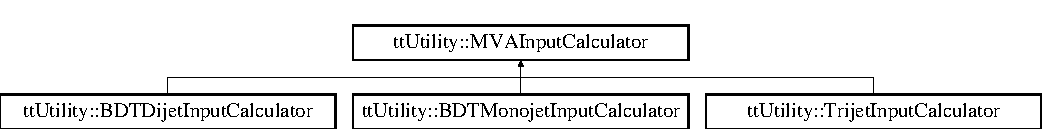
\includegraphics[height=1.728395cm]{classttUtility_1_1MVAInputCalculator}
\end{center}
\end{figure}
\subsection*{Public Member Functions}
\begin{DoxyCompactItemize}
\item 
virtual void \hyperlink{classttUtility_1_1MVAInputCalculator_aca315e5c5ce1d110660eb54cd7facfd8}{map\-Vars} (const std\-::vector$<$ std\-::string $>$ \&)=0
\item 
virtual void \hyperlink{classttUtility_1_1MVAInputCalculator_afae8a686f0fd4310a75c79216a39fa53}{set\-Ptr} (float $\ast$data)
\item 
virtual bool \hyperlink{classttUtility_1_1MVAInputCalculator_a86793cfa66ca816b2e1667a6b12db7d8}{calculate\-Vars} (const \hyperlink{classTopObject}{Top\-Object} \&, int)=0
\item 
virtual bool \hyperlink{classttUtility_1_1MVAInputCalculator_ae8df426d7943b921c0b9d086d1ccde30}{check\-Cand} (const \hyperlink{classTopObject}{Top\-Object} \&)=0
\item 
virtual \hyperlink{classttUtility_1_1MVAInputCalculator_affa17a79ff6326b86391420e29a82554}{$\sim$\-M\-V\-A\-Input\-Calculator} ()
\end{DoxyCompactItemize}
\subsection*{Protected Attributes}
\begin{DoxyCompactItemize}
\item 
\hypertarget{classttUtility_1_1MVAInputCalculator_ae7ecc7c4f0679e8adbb09104362f77e9}{float $\ast$ {\bfseries base\-Ptr\-\_\-}}\label{classttUtility_1_1MVAInputCalculator_ae7ecc7c4f0679e8adbb09104362f77e9}

\item 
\hypertarget{classttUtility_1_1MVAInputCalculator_aef257aed71b9b66adfb59b1807c8f0a4}{int {\bfseries len\-\_\-}}\label{classttUtility_1_1MVAInputCalculator_aef257aed71b9b66adfb59b1807c8f0a4}

\end{DoxyCompactItemize}


\subsection{Detailed Description}
Base class for M\-V\-A input variable calculator 

\subsection{Constructor \& Destructor Documentation}
\hypertarget{classttUtility_1_1MVAInputCalculator_affa17a79ff6326b86391420e29a82554}{\index{tt\-Utility\-::\-M\-V\-A\-Input\-Calculator@{tt\-Utility\-::\-M\-V\-A\-Input\-Calculator}!$\sim$\-M\-V\-A\-Input\-Calculator@{$\sim$\-M\-V\-A\-Input\-Calculator}}
\index{$\sim$\-M\-V\-A\-Input\-Calculator@{$\sim$\-M\-V\-A\-Input\-Calculator}!ttUtility::MVAInputCalculator@{tt\-Utility\-::\-M\-V\-A\-Input\-Calculator}}
\subsubsection[{$\sim$\-M\-V\-A\-Input\-Calculator}]{\setlength{\rightskip}{0pt plus 5cm}virtual tt\-Utility\-::\-M\-V\-A\-Input\-Calculator\-::$\sim$\-M\-V\-A\-Input\-Calculator (
\begin{DoxyParamCaption}
{}
\end{DoxyParamCaption}
)\hspace{0.3cm}{\ttfamily [inline]}, {\ttfamily [virtual]}}}\label{classttUtility_1_1MVAInputCalculator_affa17a79ff6326b86391420e29a82554}
Base distructor to allow cleanup of derived classes when necessary 

\subsection{Member Function Documentation}
\hypertarget{classttUtility_1_1MVAInputCalculator_a86793cfa66ca816b2e1667a6b12db7d8}{\index{tt\-Utility\-::\-M\-V\-A\-Input\-Calculator@{tt\-Utility\-::\-M\-V\-A\-Input\-Calculator}!calculate\-Vars@{calculate\-Vars}}
\index{calculate\-Vars@{calculate\-Vars}!ttUtility::MVAInputCalculator@{tt\-Utility\-::\-M\-V\-A\-Input\-Calculator}}
\subsubsection[{calculate\-Vars}]{\setlength{\rightskip}{0pt plus 5cm}virtual bool tt\-Utility\-::\-M\-V\-A\-Input\-Calculator\-::calculate\-Vars (
\begin{DoxyParamCaption}
\item[{const {\bf Top\-Object} \&}]{, }
\item[{int}]{}
\end{DoxyParamCaption}
)\hspace{0.3cm}{\ttfamily [pure virtual]}}}\label{classttUtility_1_1MVAInputCalculator_a86793cfa66ca816b2e1667a6b12db7d8}
Calculate the requested variables and store the values directly in the input array for the M\-V\-A 
\begin{DoxyParams}{Parameters}
{\em top\-Cand} & the top candidate to calculate the input variables for \\
\hline
\end{DoxyParams}


Implemented in \hyperlink{classttUtility_1_1TrijetInputCalculator_ab691e5a8ecd3698a609b34b6e6aff20d}{tt\-Utility\-::\-Trijet\-Input\-Calculator}, \hyperlink{classttUtility_1_1BDTDijetInputCalculator_aabe1eff89a230cc1a02606eaadc74fdc}{tt\-Utility\-::\-B\-D\-T\-Dijet\-Input\-Calculator}, and \hyperlink{classttUtility_1_1BDTMonojetInputCalculator_ade65c192d67eb363a4b4028b4f0ec7c5}{tt\-Utility\-::\-B\-D\-T\-Monojet\-Input\-Calculator}.

\hypertarget{classttUtility_1_1MVAInputCalculator_ae8df426d7943b921c0b9d086d1ccde30}{\index{tt\-Utility\-::\-M\-V\-A\-Input\-Calculator@{tt\-Utility\-::\-M\-V\-A\-Input\-Calculator}!check\-Cand@{check\-Cand}}
\index{check\-Cand@{check\-Cand}!ttUtility::MVAInputCalculator@{tt\-Utility\-::\-M\-V\-A\-Input\-Calculator}}
\subsubsection[{check\-Cand}]{\setlength{\rightskip}{0pt plus 5cm}virtual bool tt\-Utility\-::\-M\-V\-A\-Input\-Calculator\-::check\-Cand (
\begin{DoxyParamCaption}
\item[{const {\bf Top\-Object} \&}]{}
\end{DoxyParamCaption}
)\hspace{0.3cm}{\ttfamily [pure virtual]}}}\label{classttUtility_1_1MVAInputCalculator_ae8df426d7943b921c0b9d086d1ccde30}
Check if the \hyperlink{classTopObject}{Top\-Object} passes basic selection for this category. 
\begin{DoxyParams}{Parameters}
{\em top\-Cand} & the top candidate to check \\
\hline
\end{DoxyParams}


Implemented in \hyperlink{classttUtility_1_1TrijetInputCalculator_abeb8edb896b264a185a2f37747a97912}{tt\-Utility\-::\-Trijet\-Input\-Calculator}, \hyperlink{classttUtility_1_1BDTDijetInputCalculator_a2832dae8ebcb1572c05379776c67d4ef}{tt\-Utility\-::\-B\-D\-T\-Dijet\-Input\-Calculator}, and \hyperlink{classttUtility_1_1BDTMonojetInputCalculator_aabe30d40a85c15a5c4df89f39b44be88}{tt\-Utility\-::\-B\-D\-T\-Monojet\-Input\-Calculator}.

\hypertarget{classttUtility_1_1MVAInputCalculator_aca315e5c5ce1d110660eb54cd7facfd8}{\index{tt\-Utility\-::\-M\-V\-A\-Input\-Calculator@{tt\-Utility\-::\-M\-V\-A\-Input\-Calculator}!map\-Vars@{map\-Vars}}
\index{map\-Vars@{map\-Vars}!ttUtility::MVAInputCalculator@{tt\-Utility\-::\-M\-V\-A\-Input\-Calculator}}
\subsubsection[{map\-Vars}]{\setlength{\rightskip}{0pt plus 5cm}virtual void tt\-Utility\-::\-M\-V\-A\-Input\-Calculator\-::map\-Vars (
\begin{DoxyParamCaption}
\item[{const std\-::vector$<$ std\-::string $>$ \&}]{}
\end{DoxyParamCaption}
)\hspace{0.3cm}{\ttfamily [pure virtual]}}}\label{classttUtility_1_1MVAInputCalculator_aca315e5c5ce1d110660eb54cd7facfd8}
The job of map\-Vars is to populate the internal offests for all variables in the input variable list with their memory location in the data array. To be called only once. 
\begin{DoxyParams}{Parameters}
{\em vars} & list of variables used for the model \\
\hline
\end{DoxyParams}


Implemented in \hyperlink{classttUtility_1_1TrijetInputCalculator_a22f76e3d58040a99324f6748f340a4fc}{tt\-Utility\-::\-Trijet\-Input\-Calculator}, \hyperlink{classttUtility_1_1BDTDijetInputCalculator_a8b3197ff6ced189b17e3d666ef8f24a7}{tt\-Utility\-::\-B\-D\-T\-Dijet\-Input\-Calculator}, and \hyperlink{classttUtility_1_1BDTMonojetInputCalculator_af929778a33ce64a1c5102712a2858aa0}{tt\-Utility\-::\-B\-D\-T\-Monojet\-Input\-Calculator}.

\hypertarget{classttUtility_1_1MVAInputCalculator_afae8a686f0fd4310a75c79216a39fa53}{\index{tt\-Utility\-::\-M\-V\-A\-Input\-Calculator@{tt\-Utility\-::\-M\-V\-A\-Input\-Calculator}!set\-Ptr@{set\-Ptr}}
\index{set\-Ptr@{set\-Ptr}!ttUtility::MVAInputCalculator@{tt\-Utility\-::\-M\-V\-A\-Input\-Calculator}}
\subsubsection[{set\-Ptr}]{\setlength{\rightskip}{0pt plus 5cm}virtual void tt\-Utility\-::\-M\-V\-A\-Input\-Calculator\-::set\-Ptr (
\begin{DoxyParamCaption}
\item[{float $\ast$}]{data}
\end{DoxyParamCaption}
)\hspace{0.3cm}{\ttfamily [inline]}, {\ttfamily [virtual]}}}\label{classttUtility_1_1MVAInputCalculator_afae8a686f0fd4310a75c79216a39fa53}
The job of set\-Ptr is to set hte starting place of memory block where the data will be written. To be called only once for the creation of the array pointed to by data. 
\begin{DoxyParams}{Parameters}
{\em data} & pointer to start of the data array which will be used as input to the M\-V\-A \\
\hline
\end{DoxyParams}


The documentation for this class was generated from the following file\-:\begin{DoxyCompactItemize}
\item 
/home/travis/build/susy2015/\-Top\-Tagger/\-Top\-Tagger/include/\hyperlink{TopTaggerUtilities_8h}{Top\-Tagger\-Utilities.\-h}\end{DoxyCompactItemize}

\hypertarget{classtaggerOptions_1_1networkOptions}{\section{tagger\-Options.\-network\-Options Class Reference}
\label{classtaggerOptions_1_1networkOptions}\index{tagger\-Options.\-network\-Options@{tagger\-Options.\-network\-Options}}
}


The documentation for this class was generated from the following file\-:\begin{DoxyCompactItemize}
\item 
/home/travis/build/susy2015/\-Top\-Tagger/\-Tools/python/tagger\-Options.\-py\end{DoxyCompactItemize}

\hypertarget{classcfg_1_1Parameter}{\section{cfg\-:\-:Parameter Class Reference}
\label{classcfg_1_1Parameter}\index{cfg\-::\-Parameter@{cfg\-::\-Parameter}}
}
\subsection*{Public Member Functions}
\begin{DoxyCompactItemize}
\item 
\hypertarget{classcfg_1_1Parameter_a208c448cc6de79567c2b2259249c8a79}{{\bfseries Parameter} (const std\-::string \&ns, const std\-::string \&name)}\label{classcfg_1_1Parameter_a208c448cc6de79567c2b2259249c8a79}

\item 
\hypertarget{classcfg_1_1Parameter_accc34a74932a723a9b49d549d9809708}{void {\bfseries add\-Assignment} (const \hyperlink{classcfg_1_1ConditionChain}{Condition\-Chain} \&c, const \hyperlink{classcfg_1_1Literal}{Literal} \&val)}\label{classcfg_1_1Parameter_accc34a74932a723a9b49d549d9809708}

\item 
\hypertarget{classcfg_1_1Parameter_a7d842ced7fa8103fa930eeb69707d1a9}{\hyperlink{classcfg_1_1Literal}{Literal} {\bfseries value\-In\-Context} (const \hyperlink{classcfg_1_1Context}{Context} \&cxt, bool exception\-Missing=false) const }\label{classcfg_1_1Parameter_a7d842ced7fa8103fa930eeb69707d1a9}

\item 
\hypertarget{classcfg_1_1Parameter_a5dbc324f94e7096a3b6cbcaafd3ffd39}{const std\-::string \& {\bfseries name} () const }\label{classcfg_1_1Parameter_a5dbc324f94e7096a3b6cbcaafd3ffd39}

\item 
\hypertarget{classcfg_1_1Parameter_a53bb1d90e0de3cbe2b7385723e8dc097}{const std\-::string \& {\bfseries ns} () const }\label{classcfg_1_1Parameter_a53bb1d90e0de3cbe2b7385723e8dc097}

\item 
\hypertarget{classcfg_1_1Parameter_a29f1055709d780e898fac6c110295ed1}{std\-::set$<$ std\-::string $>$ {\bfseries conditional\-Items} () const }\label{classcfg_1_1Parameter_a29f1055709d780e898fac6c110295ed1}

\end{DoxyCompactItemize}


The documentation for this class was generated from the following files\-:\begin{DoxyCompactItemize}
\item 
/home/travis/build/susy2015/\-Top\-Tagger/\-Cfg\-Parser/include/Parameter.\-hh\item 
/home/travis/build/susy2015/\-Top\-Tagger/\-Cfg\-Parser/src/Parameter.\-cc\end{DoxyCompactItemize}

\hypertarget{classhcalcfg_1_1Parser}{\section{hcalcfg\-:\-:Parser Class Reference}
\label{classhcalcfg_1_1Parser}\index{hcalcfg\-::\-Parser@{hcalcfg\-::\-Parser}}
}
\subsection*{Public Member Functions}
\begin{DoxyCompactItemize}
\item 
\hypertarget{classhcalcfg_1_1Parser_a8d9293499bffa2afca86df359dfb4fbf}{{\bfseries Parser} (\hyperlink{classhcalcfg_1_1Scanner}{Scanner} $\ast$scanner)}\label{classhcalcfg_1_1Parser_a8d9293499bffa2afca86df359dfb4fbf}

\item 
\hypertarget{classhcalcfg_1_1Parser_a5f92e06aec420485a4530d2da45e1e00}{void {\bfseries Sem\-Err} (const wchar\-\_\-t $\ast$msg)}\label{classhcalcfg_1_1Parser_a5f92e06aec420485a4530d2da45e1e00}

\item 
\hypertarget{classhcalcfg_1_1Parser_ad5f7b94128a1804bae0d02618238c9f6}{void {\bfseries Hcal\-Cfg} ()}\label{classhcalcfg_1_1Parser_ad5f7b94128a1804bae0d02618238c9f6}

\item 
\hypertarget{classhcalcfg_1_1Parser_a967925b9ca68f60cfb7a133851c2c442}{void {\bfseries Line} ()}\label{classhcalcfg_1_1Parser_a967925b9ca68f60cfb7a133851c2c442}

\item 
\hypertarget{classhcalcfg_1_1Parser_ab4c4f7f234fea3c4f9ee8004123288a3}{void {\bfseries Global\-Conditional} ()}\label{classhcalcfg_1_1Parser_ab4c4f7f234fea3c4f9ee8004123288a3}

\item 
\hypertarget{classhcalcfg_1_1Parser_a18f5fcbd06a829818654f24379c13e59}{void {\bfseries Group\-Def} ()}\label{classhcalcfg_1_1Parser_a18f5fcbd06a829818654f24379c13e59}

\item 
\hypertarget{classhcalcfg_1_1Parser_a6f193b9198c8834fea5f2125390be5b3}{void {\bfseries Compound\-I\-C} ()}\label{classhcalcfg_1_1Parser_a6f193b9198c8834fea5f2125390be5b3}

\item 
\hypertarget{classhcalcfg_1_1Parser_a51ddf3d7fc2a96ba699ee6bbe747f817}{void {\bfseries Simple\-I\-C} ()}\label{classhcalcfg_1_1Parser_a51ddf3d7fc2a96ba699ee6bbe747f817}

\item 
\hypertarget{classhcalcfg_1_1Parser_a5fef141a6785e8f3a639186dc18ace9e}{void {\bfseries Assign\-Or\-Cond} ()}\label{classhcalcfg_1_1Parser_a5fef141a6785e8f3a639186dc18ace9e}

\item 
\hypertarget{classhcalcfg_1_1Parser_a2c4e2bd96ccff681c1d32bbe2f3859d3}{void {\bfseries Assign} ()}\label{classhcalcfg_1_1Parser_a2c4e2bd96ccff681c1d32bbe2f3859d3}

\item 
void \hyperlink{classhcalcfg_1_1Parser_aff2144d6e73f4970871d14fdec652d0f}{Conditional\-Assign} ()
\item 
void \hyperlink{classhcalcfg_1_1Parser_a02830a58b2fe792ad11954827cf46312}{Item} ()
\item 
\hypertarget{classhcalcfg_1_1Parser_a6d9e3c01a17aab5ac38e8ea2b5c961f0}{void {\bfseries Literal} ()}\label{classhcalcfg_1_1Parser_a6d9e3c01a17aab5ac38e8ea2b5c961f0}

\item 
\hypertarget{classhcalcfg_1_1Parser_ad72ade9f20c2c0bc360adf012637e070}{void {\bfseries Compound\-Term} (\hyperlink{classcfg_1_1TermAnd}{cfg\-::\-Term\-And} \&at)}\label{classhcalcfg_1_1Parser_ad72ade9f20c2c0bc360adf012637e070}

\item 
\hypertarget{classhcalcfg_1_1Parser_a4b1088b96598a1fd50e3f350bcd4da34}{void {\bfseries Term} (\hyperlink{classcfg_1_1SimpleTerm}{cfg\-::\-Simple\-Term} $\ast$\&term)}\label{classhcalcfg_1_1Parser_a4b1088b96598a1fd50e3f350bcd4da34}

\item 
\hypertarget{classhcalcfg_1_1Parser_ad73ac339e91080292d12ee20a7f60b10}{void {\bfseries List} ()}\label{classhcalcfg_1_1Parser_ad73ac339e91080292d12ee20a7f60b10}

\item 
\hypertarget{classhcalcfg_1_1Parser_ae6476241f0b7fd642add79825c0da163}{void {\bfseries Parse} ()}\label{classhcalcfg_1_1Parser_ae6476241f0b7fd642add79825c0da163}

\end{DoxyCompactItemize}
\subsection*{Public Attributes}
\begin{DoxyCompactItemize}
\item 
\hypertarget{classhcalcfg_1_1Parser_aef6a9818311b7fb3776dca358bfffc7b}{\hyperlink{classhcalcfg_1_1Scanner}{Scanner} $\ast$ {\bfseries scanner}}\label{classhcalcfg_1_1Parser_aef6a9818311b7fb3776dca358bfffc7b}

\item 
\hypertarget{classhcalcfg_1_1Parser_a99f438957c96c39d7031ce6c9e517081}{\hyperlink{classhcalcfg_1_1Errors}{Errors} $\ast$ {\bfseries errors}}\label{classhcalcfg_1_1Parser_a99f438957c96c39d7031ce6c9e517081}

\item 
\hypertarget{classhcalcfg_1_1Parser_a2de4346ebb4cd79b1141f9c8037fbd1e}{\hyperlink{classhcalcfg_1_1Token}{Token} $\ast$ {\bfseries t}}\label{classhcalcfg_1_1Parser_a2de4346ebb4cd79b1141f9c8037fbd1e}

\item 
\hypertarget{classhcalcfg_1_1Parser_a8d04489fae1ee514e667885c49c63a78}{\hyperlink{classhcalcfg_1_1Token}{Token} $\ast$ {\bfseries la}}\label{classhcalcfg_1_1Parser_a8d04489fae1ee514e667885c49c63a78}

\item 
\hypertarget{classhcalcfg_1_1Parser_a6658979da28569d4f52183c0ec667900}{\hyperlink{classCfgBuilder}{Cfg\-Builder} {\bfseries m\-\_\-builder}}\label{classhcalcfg_1_1Parser_a6658979da28569d4f52183c0ec667900}

\end{DoxyCompactItemize}


\subsection{Member Function Documentation}
\hypertarget{classhcalcfg_1_1Parser_aff2144d6e73f4970871d14fdec652d0f}{\index{hcalcfg\-::\-Parser@{hcalcfg\-::\-Parser}!Conditional\-Assign@{Conditional\-Assign}}
\index{Conditional\-Assign@{Conditional\-Assign}!hcalcfg::Parser@{hcalcfg\-::\-Parser}}
\subsubsection[{Conditional\-Assign}]{\setlength{\rightskip}{0pt plus 5cm}void hcalcfg\-::\-Parser\-::\-Conditional\-Assign (
\begin{DoxyParamCaption}
{}
\end{DoxyParamCaption}
)}}\label{classhcalcfg_1_1Parser_aff2144d6e73f4970871d14fdec652d0f}
(E\-O\-F $\vert$$\vert$ ')' ) \hypertarget{classhcalcfg_1_1Parser_a02830a58b2fe792ad11954827cf46312}{\index{hcalcfg\-::\-Parser@{hcalcfg\-::\-Parser}!Item@{Item}}
\index{Item@{Item}!hcalcfg::Parser@{hcalcfg\-::\-Parser}}
\subsubsection[{Item}]{\setlength{\rightskip}{0pt plus 5cm}void hcalcfg\-::\-Parser\-::\-Item (
\begin{DoxyParamCaption}
{}
\end{DoxyParamCaption}
)}}\label{classhcalcfg_1_1Parser_a02830a58b2fe792ad11954827cf46312}
( E\-O\-F $\vert$$\vert$ \mbox{]} ) 

The documentation for this class was generated from the following files\-:\begin{DoxyCompactItemize}
\item 
/home/travis/build/susy2015/\-Top\-Tagger/\-Cfg\-Parser/include/Parser.\-h\item 
/home/travis/build/susy2015/\-Top\-Tagger/\-Cfg\-Parser/src/Parser.\-cpp\end{DoxyCompactItemize}

\hypertarget{structhcalcfg_1_1ParserDestroyCaller}{\section{hcalcfg\-:\-:Parser\-Destroy\-Caller$<$ T, bool $>$ Struct Template Reference}
\label{structhcalcfg_1_1ParserDestroyCaller}\index{hcalcfg\-::\-Parser\-Destroy\-Caller$<$ T, bool $>$@{hcalcfg\-::\-Parser\-Destroy\-Caller$<$ T, bool $>$}}
}
\subsection*{Static Public Member Functions}
\begin{DoxyCompactItemize}
\item 
\hypertarget{structhcalcfg_1_1ParserDestroyCaller_a7b6573874f65985b4a1a5d5cb1a5e449}{static void {\bfseries Call\-Destroy} (T $\ast$t)}\label{structhcalcfg_1_1ParserDestroyCaller_a7b6573874f65985b4a1a5d5cb1a5e449}

\end{DoxyCompactItemize}


The documentation for this struct was generated from the following file\-:\begin{DoxyCompactItemize}
\item 
/home/travis/build/susy2015/\-Top\-Tagger/\-Cfg\-Parser/src/Parser.\-cpp\end{DoxyCompactItemize}

\hypertarget{structhcalcfg_1_1ParserDestroyCaller_3_01T_00_01true_01_4}{\section{hcalcfg\-:\-:Parser\-Destroy\-Caller$<$ T, true $>$ Struct Template Reference}
\label{structhcalcfg_1_1ParserDestroyCaller_3_01T_00_01true_01_4}\index{hcalcfg\-::\-Parser\-Destroy\-Caller$<$ T, true $>$@{hcalcfg\-::\-Parser\-Destroy\-Caller$<$ T, true $>$}}
}
\subsection*{Static Public Member Functions}
\begin{DoxyCompactItemize}
\item 
\hypertarget{structhcalcfg_1_1ParserDestroyCaller_3_01T_00_01true_01_4_a5e154cf10500ccf96696697c6aafe244}{static void {\bfseries Call\-Destroy} (T $\ast$t)}\label{structhcalcfg_1_1ParserDestroyCaller_3_01T_00_01true_01_4_a5e154cf10500ccf96696697c6aafe244}

\end{DoxyCompactItemize}


The documentation for this struct was generated from the following file\-:\begin{DoxyCompactItemize}
\item 
/home/travis/build/susy2015/\-Top\-Tagger/\-Cfg\-Parser/src/Parser.\-cpp\end{DoxyCompactItemize}

\hypertarget{structhcalcfg_1_1ParserDestroyExistsRecognizer}{\section{hcalcfg\-:\-:Parser\-Destroy\-Exists\-Recognizer$<$ T $>$ Struct Template Reference}
\label{structhcalcfg_1_1ParserDestroyExistsRecognizer}\index{hcalcfg\-::\-Parser\-Destroy\-Exists\-Recognizer$<$ T $>$@{hcalcfg\-::\-Parser\-Destroy\-Exists\-Recognizer$<$ T $>$}}
}
\subsection*{Classes}
\begin{DoxyCompactItemize}
\item 
struct \hyperlink{structhcalcfg_1_1ParserDestroyExistsRecognizer_1_1DestroyExistsType}{Destroy\-Exists\-Type}
\item 
struct \hyperlink{structhcalcfg_1_1ParserDestroyExistsRecognizer_1_1DestroyIsMissingType}{Destroy\-Is\-Missing\-Type}
\item 
struct \hyperlink{structhcalcfg_1_1ParserDestroyExistsRecognizer_1_1ExistsIfDestroyIsDefinedMarker}{Exists\-If\-Destroy\-Is\-Defined\-Marker}
\end{DoxyCompactItemize}
\subsection*{Public Types}
\begin{DoxyCompactItemize}
\item 
enum \{ {\bfseries Destroy\-Exists} = (sizeof(is\-\_\-here$<$T$>$(N\-U\-L\-L)) == sizeof(Destroy\-Exists\-Type))
 \}
\end{DoxyCompactItemize}
\subsection*{Static Public Member Functions}
\begin{DoxyCompactItemize}
\item 
\hypertarget{structhcalcfg_1_1ParserDestroyExistsRecognizer_af68a10598ce38579f5c9a2fa9fb50d3a}{{\footnotesize template$<$typename U $>$ }\\static \hyperlink{structhcalcfg_1_1ParserDestroyExistsRecognizer_1_1DestroyIsMissingType}{Destroy\-Is\-Missing\-Type} {\bfseries is\-\_\-here} (...)}\label{structhcalcfg_1_1ParserDestroyExistsRecognizer_af68a10598ce38579f5c9a2fa9fb50d3a}

\item 
\hypertarget{structhcalcfg_1_1ParserDestroyExistsRecognizer_a91e99c149cfc18d4d3ba65efd2eb41ef}{{\footnotesize template$<$typename U $>$ }\\static \hyperlink{structhcalcfg_1_1ParserDestroyExistsRecognizer_1_1DestroyExistsType}{Destroy\-Exists\-Type} {\bfseries is\-\_\-here} (\hyperlink{structhcalcfg_1_1ParserDestroyExistsRecognizer_1_1ExistsIfDestroyIsDefinedMarker}{Exists\-If\-Destroy\-Is\-Defined\-Marker}$<$ U $>$ $\ast$)}\label{structhcalcfg_1_1ParserDestroyExistsRecognizer_a91e99c149cfc18d4d3ba65efd2eb41ef}

\end{DoxyCompactItemize}


The documentation for this struct was generated from the following file\-:\begin{DoxyCompactItemize}
\item 
/home/travis/build/susy2015/\-Top\-Tagger/\-Cfg\-Parser/src/Parser.\-cpp\end{DoxyCompactItemize}

\hypertarget{structhcalcfg_1_1ParserInitCaller}{\section{hcalcfg\-:\-:Parser\-Init\-Caller$<$ T, bool $>$ Struct Template Reference}
\label{structhcalcfg_1_1ParserInitCaller}\index{hcalcfg\-::\-Parser\-Init\-Caller$<$ T, bool $>$@{hcalcfg\-::\-Parser\-Init\-Caller$<$ T, bool $>$}}
}
\subsection*{Static Public Member Functions}
\begin{DoxyCompactItemize}
\item 
\hypertarget{structhcalcfg_1_1ParserInitCaller_acf35f0c5780c9b92f444a4ffec906629}{static void {\bfseries Call\-Init} (T $\ast$t)}\label{structhcalcfg_1_1ParserInitCaller_acf35f0c5780c9b92f444a4ffec906629}

\end{DoxyCompactItemize}


The documentation for this struct was generated from the following file\-:\begin{DoxyCompactItemize}
\item 
/home/travis/build/susy2015/\-Top\-Tagger/\-Cfg\-Parser/src/Parser.\-cpp\end{DoxyCompactItemize}

\hypertarget{structhcalcfg_1_1ParserInitCaller_3_01T_00_01true_01_4}{\section{hcalcfg\-:\-:Parser\-Init\-Caller$<$ T, true $>$ Struct Template Reference}
\label{structhcalcfg_1_1ParserInitCaller_3_01T_00_01true_01_4}\index{hcalcfg\-::\-Parser\-Init\-Caller$<$ T, true $>$@{hcalcfg\-::\-Parser\-Init\-Caller$<$ T, true $>$}}
}
\subsection*{Static Public Member Functions}
\begin{DoxyCompactItemize}
\item 
\hypertarget{structhcalcfg_1_1ParserInitCaller_3_01T_00_01true_01_4_ab62af8f09bde031e594df3766f45f9da}{static void {\bfseries Call\-Init} (T $\ast$t)}\label{structhcalcfg_1_1ParserInitCaller_3_01T_00_01true_01_4_ab62af8f09bde031e594df3766f45f9da}

\end{DoxyCompactItemize}


The documentation for this struct was generated from the following file\-:\begin{DoxyCompactItemize}
\item 
/home/travis/build/susy2015/\-Top\-Tagger/\-Cfg\-Parser/src/Parser.\-cpp\end{DoxyCompactItemize}

\hypertarget{structhcalcfg_1_1ParserInitExistsRecognizer}{\section{hcalcfg\-:\-:Parser\-Init\-Exists\-Recognizer$<$ T $>$ Struct Template Reference}
\label{structhcalcfg_1_1ParserInitExistsRecognizer}\index{hcalcfg\-::\-Parser\-Init\-Exists\-Recognizer$<$ T $>$@{hcalcfg\-::\-Parser\-Init\-Exists\-Recognizer$<$ T $>$}}
}
\subsection*{Classes}
\begin{DoxyCompactItemize}
\item 
struct \hyperlink{structhcalcfg_1_1ParserInitExistsRecognizer_1_1ExistsIfInitIsDefinedMarker}{Exists\-If\-Init\-Is\-Defined\-Marker}
\item 
struct \hyperlink{structhcalcfg_1_1ParserInitExistsRecognizer_1_1InitExistsType}{Init\-Exists\-Type}
\item 
struct \hyperlink{structhcalcfg_1_1ParserInitExistsRecognizer_1_1InitIsMissingType}{Init\-Is\-Missing\-Type}
\end{DoxyCompactItemize}
\subsection*{Public Types}
\begin{DoxyCompactItemize}
\item 
enum \{ {\bfseries Init\-Exists} = (sizeof(is\-\_\-here$<$T$>$(N\-U\-L\-L)) == sizeof(Init\-Exists\-Type))
 \}
\end{DoxyCompactItemize}
\subsection*{Static Public Member Functions}
\begin{DoxyCompactItemize}
\item 
\hypertarget{structhcalcfg_1_1ParserInitExistsRecognizer_aadde7f9eaac716099eb3c14007f85c6b}{{\footnotesize template$<$typename U $>$ }\\static \hyperlink{structhcalcfg_1_1ParserInitExistsRecognizer_1_1InitIsMissingType}{Init\-Is\-Missing\-Type} {\bfseries is\-\_\-here} (...)}\label{structhcalcfg_1_1ParserInitExistsRecognizer_aadde7f9eaac716099eb3c14007f85c6b}

\item 
\hypertarget{structhcalcfg_1_1ParserInitExistsRecognizer_af638bb614f5dcd2848c4b7e85d3f8a4e}{{\footnotesize template$<$typename U $>$ }\\static \hyperlink{structhcalcfg_1_1ParserInitExistsRecognizer_1_1InitExistsType}{Init\-Exists\-Type} {\bfseries is\-\_\-here} (\hyperlink{structhcalcfg_1_1ParserInitExistsRecognizer_1_1ExistsIfInitIsDefinedMarker}{Exists\-If\-Init\-Is\-Defined\-Marker}$<$ U $>$ $\ast$)}\label{structhcalcfg_1_1ParserInitExistsRecognizer_af638bb614f5dcd2848c4b7e85d3f8a4e}

\end{DoxyCompactItemize}


The documentation for this struct was generated from the following file\-:\begin{DoxyCompactItemize}
\item 
/home/travis/build/susy2015/\-Top\-Tagger/\-Cfg\-Parser/src/Parser.\-cpp\end{DoxyCompactItemize}

\hypertarget{classrocPlot_1_1Plotter}{\section{roc\-Plot.\-Plotter Class Reference}
\label{classrocPlot_1_1Plotter}\index{roc\-Plot.\-Plotter@{roc\-Plot.\-Plotter}}
}
\subsection*{Public Member Functions}
\begin{DoxyCompactItemize}
\item 
\hypertarget{classrocPlot_1_1Plotter_a3340e985d0711bb2a87483b329abbd1e}{def {\bfseries \-\_\-\-\_\-init\-\_\-\-\_\-}}\label{classrocPlot_1_1Plotter_a3340e985d0711bb2a87483b329abbd1e}

\end{DoxyCompactItemize}
\subsection*{Public Attributes}
\begin{DoxyCompactItemize}
\item 
\hypertarget{classrocPlot_1_1Plotter_ae2e857d10e07a3acf5e5ab88812ed908}{{\bfseries output\-Directory}}\label{classrocPlot_1_1Plotter_ae2e857d10e07a3acf5e5ab88812ed908}

\item 
\hypertarget{classrocPlot_1_1Plotter_a4662c882aa24d845e93f369b5951ddaf}{{\bfseries json\-File}}\label{classrocPlot_1_1Plotter_a4662c882aa24d845e93f369b5951ddaf}

\item 
\hypertarget{classrocPlot_1_1Plotter_a9df7daadc166d1c230ca4821a1c0de96}{{\bfseries colors}}\label{classrocPlot_1_1Plotter_a9df7daadc166d1c230ca4821a1c0de96}

\end{DoxyCompactItemize}


The documentation for this class was generated from the following file\-:\begin{DoxyCompactItemize}
\item 
/home/travis/build/susy2015/\-Top\-Tagger/\-Tools/python/roc\-Plot.\-py\end{DoxyCompactItemize}

\hypertarget{classPrepVariables}{\section{Prep\-Variables Class Reference}
\label{classPrepVariables}\index{Prep\-Variables@{Prep\-Variables}}
}
\subsection*{Public Member Functions}
\begin{DoxyCompactItemize}
\item 
\hypertarget{classPrepVariables_a347b319c24242ecda7f705b96ca29199}{std\-::set$<$ std\-::string $>$ {\bfseries get\-Var\-Set} ()}\label{classPrepVariables_a347b319c24242ecda7f705b96ca29199}

\item 
\hypertarget{classPrepVariables_aed38f9b1b9087c13d9380b04ab6c598e}{void {\bfseries operator()} (N\-Tuple\-Reader \&tr)}\label{classPrepVariables_aed38f9b1b9087c13d9380b04ab6c598e}

\end{DoxyCompactItemize}


The documentation for this class was generated from the following file\-:\begin{DoxyCompactItemize}
\item 
/home/travis/build/susy2015/\-Top\-Tagger/\-Tools/cpp/make\-Training\-Tuples.\-C\end{DoxyCompactItemize}

\hypertarget{classttPython_1_1Py__buffer__wrapper}{\section{tt\-Python\-:\-:Py\-\_\-buffer\-\_\-wrapper$<$ T $>$ Class Template Reference}
\label{classttPython_1_1Py__buffer__wrapper}\index{tt\-Python\-::\-Py\-\_\-buffer\-\_\-wrapper$<$ T $>$@{tt\-Python\-::\-Py\-\_\-buffer\-\_\-wrapper$<$ T $>$}}
}


{\ttfamily \#include $<$Top\-Tagger\-Python.\-h$>$}

\subsection*{Public Member Functions}
\begin{DoxyCompactItemize}
\item 
\hypertarget{classttPython_1_1Py__buffer__wrapper_a56901c5eaa03f74d09575553ba694c02}{{\bfseries Py\-\_\-buffer\-\_\-wrapper} (void $\ast$buf)}\label{classttPython_1_1Py__buffer__wrapper_a56901c5eaa03f74d09575553ba694c02}

\item 
\hypertarget{classttPython_1_1Py__buffer__wrapper_a18101320c66c7c066866e6fda8e41116}{{\bfseries Py\-\_\-buffer\-\_\-wrapper} (\hyperlink{classttPython_1_1Py__buffer__wrapper}{Py\-\_\-buffer\-\_\-wrapper} \&)=delete}\label{classttPython_1_1Py__buffer__wrapper_a18101320c66c7c066866e6fda8e41116}

\item 
\hypertarget{classttPython_1_1Py__buffer__wrapper_aed14786291095cbd9aa1fd3c5f68ac1a}{{\bfseries Py\-\_\-buffer\-\_\-wrapper} (\hyperlink{classttPython_1_1Py__buffer__wrapper}{Py\-\_\-buffer\-\_\-wrapper} \&\&old)}\label{classttPython_1_1Py__buffer__wrapper_aed14786291095cbd9aa1fd3c5f68ac1a}

\item 
\hypertarget{classttPython_1_1Py__buffer__wrapper_a7ba53310e416a8b8a0ff56ca1568ba0b}{{\bfseries Py\-\_\-buffer\-\_\-wrapper} (std\-::vector$<$ T $>$ \&\&buf)}\label{classttPython_1_1Py__buffer__wrapper_a7ba53310e416a8b8a0ff56ca1568ba0b}

\item 
\hypertarget{classttPython_1_1Py__buffer__wrapper_a025070123ca2b75de184c42cbca24fc6}{unsigned int {\bfseries size} () const }\label{classttPython_1_1Py__buffer__wrapper_a025070123ca2b75de184c42cbca24fc6}

\item 
\hypertarget{classttPython_1_1Py__buffer__wrapper_a738aaf24bd0d1e52e559039e62cab787}{T \& {\bfseries operator\mbox{[}$\,$\mbox{]}} (unsigned int i)}\label{classttPython_1_1Py__buffer__wrapper_a738aaf24bd0d1e52e559039e62cab787}

\item 
\hypertarget{classttPython_1_1Py__buffer__wrapper_af13e3bfd741987b1823e24a7cd73a26c}{const T \& {\bfseries operator\mbox{[}$\,$\mbox{]}} (unsigned int i) const }\label{classttPython_1_1Py__buffer__wrapper_af13e3bfd741987b1823e24a7cd73a26c}

\item 
\hypertarget{classttPython_1_1Py__buffer__wrapper_a0fa992161236e4454b167740b6e30b97}{T $\ast$ {\bfseries begin} ()}\label{classttPython_1_1Py__buffer__wrapper_a0fa992161236e4454b167740b6e30b97}

\item 
\hypertarget{classttPython_1_1Py__buffer__wrapper_aeacb1dc0fe90db32455f27643881540f}{const T $\ast$ {\bfseries begin} () const }\label{classttPython_1_1Py__buffer__wrapper_aeacb1dc0fe90db32455f27643881540f}

\item 
\hypertarget{classttPython_1_1Py__buffer__wrapper_a41c4971f28ee2ed808d5250b5c47bbc2}{T $\ast$ {\bfseries end} ()}\label{classttPython_1_1Py__buffer__wrapper_a41c4971f28ee2ed808d5250b5c47bbc2}

\item 
\hypertarget{classttPython_1_1Py__buffer__wrapper_a7670be3ca39ee4cd6756ee324f54e554}{const T $\ast$ {\bfseries end} () const }\label{classttPython_1_1Py__buffer__wrapper_a7670be3ca39ee4cd6756ee324f54e554}

\end{DoxyCompactItemize}


\subsection{Detailed Description}
\subsubsection*{template$<$typename T$>$class tt\-Python\-::\-Py\-\_\-buffer\-\_\-wrapper$<$ T $>$}

Wrapper class to take a Py\-\_\-buffer$\ast$ and hold it in a vector-\/like implementation for use in tt\-Utilities classes. Overloaded constructor for use with vectors. In both the case of the Py\-Buffer and std\-::vector it is the users responcibility to ensure that the memory pass into this wrapper stays in scope until the wrapper is destroyed . 

The documentation for this class was generated from the following file\-:\begin{DoxyCompactItemize}
\item 
/home/travis/build/susy2015/\-Top\-Tagger/\-Top\-Tagger/interface/Top\-Tagger\-Python.\-h\end{DoxyCompactItemize}

\hypertarget{classcfg_1_1Record}{\section{cfg\-:\-:Record Class Reference}
\label{classcfg_1_1Record}\index{cfg\-::\-Record@{cfg\-::\-Record}}
}
\subsection*{Public Types}
\begin{DoxyCompactItemize}
\item 
\hypertarget{classcfg_1_1Record_a4dfe770255cb176de77eca94b9f6ebc1}{typedef std\-::map$<$ std\-::string, \\*
\hyperlink{classcfg_1_1Literal}{Literal} $>$ {\bfseries item\-\_\-collection}}\label{classcfg_1_1Record_a4dfe770255cb176de77eca94b9f6ebc1}

\item 
\hypertarget{classcfg_1_1Record_a1a263360dc1953308854186fa7504a21}{typedef std\-::map$<$ std\-::string, \\*
\hyperlink{classcfg_1_1Literal}{Literal} $>$\-::const\-\_\-iterator {\bfseries const\-\_\-item\-\_\-iterator}}\label{classcfg_1_1Record_a1a263360dc1953308854186fa7504a21}

\item 
\hypertarget{classcfg_1_1Record_a7bd66456e3235536514e29b88a7944aa}{typedef std\-::map$<$ std\-::string, \\*
\hyperlink{classcfg_1_1Literal}{Literal} $>$\-::iterator {\bfseries item\-\_\-iterator}}\label{classcfg_1_1Record_a7bd66456e3235536514e29b88a7944aa}

\end{DoxyCompactItemize}
\subsection*{Public Member Functions}
\begin{DoxyCompactItemize}
\item 
\hypertarget{classcfg_1_1Record_a85c09621795cf3542ec763d6327e81c4}{void {\bfseries record} (const \hyperlink{classcfg_1_1Context}{Context} \&cxt, const std\-::string \&item, const \hyperlink{classcfg_1_1Literal}{Literal} \&val, bool is\-Default=false)}\label{classcfg_1_1Record_a85c09621795cf3542ec763d6327e81c4}

\item 
\hypertarget{classcfg_1_1Record_ae8210318331d2c74c02d215f30fc342e}{const\-\_\-item\-\_\-iterator {\bfseries item\-\_\-begin} (const \hyperlink{classcfg_1_1Context}{Context} \&cxt) const }\label{classcfg_1_1Record_ae8210318331d2c74c02d215f30fc342e}

\item 
\hypertarget{classcfg_1_1Record_ad64483c0ec534a36d9ea84ea53250005}{const\-\_\-item\-\_\-iterator {\bfseries item\-\_\-end} (const \hyperlink{classcfg_1_1Context}{Context} \&cxt) const }\label{classcfg_1_1Record_ad64483c0ec534a36d9ea84ea53250005}

\item 
\hypertarget{classcfg_1_1Record_a391f99fe29ec058075b6810b1b14ca3f}{bool {\bfseries was\-Default} (const \hyperlink{classcfg_1_1Context}{Context} \&cxt, const std\-::string \&item) const }\label{classcfg_1_1Record_a391f99fe29ec058075b6810b1b14ca3f}

\item 
\hypertarget{classcfg_1_1Record_a0808d25ac6925c9acc7acf9411c5db17}{std\-::vector$<$ \hyperlink{classcfg_1_1Context}{Context} $>$ {\bfseries contexts} () const }\label{classcfg_1_1Record_a0808d25ac6925c9acc7acf9411c5db17}

\end{DoxyCompactItemize}


The documentation for this class was generated from the following files\-:\begin{DoxyCompactItemize}
\item 
/home/travis/build/susy2015/\-Top\-Tagger/\-Cfg\-Parser/include/Record.\-hh\item 
/home/travis/build/susy2015/\-Top\-Tagger/\-Cfg\-Parser/src/Record.\-cc\end{DoxyCompactItemize}

\hypertarget{classtaggerOptions_1_1runOptions}{\section{tagger\-Options.\-run\-Options Class Reference}
\label{classtaggerOptions_1_1runOptions}\index{tagger\-Options.\-run\-Options@{tagger\-Options.\-run\-Options}}
}


The documentation for this class was generated from the following file\-:\begin{DoxyCompactItemize}
\item 
/home/travis/build/susy2015/\-Top\-Tagger/\-Tools/python/tagger\-Options.\-py\end{DoxyCompactItemize}

\hypertarget{classhcalcfg_1_1Scanner}{\section{hcalcfg\-:\-:Scanner Class Reference}
\label{classhcalcfg_1_1Scanner}\index{hcalcfg\-::\-Scanner@{hcalcfg\-::\-Scanner}}
}
\subsection*{Public Member Functions}
\begin{DoxyCompactItemize}
\item 
\hypertarget{classhcalcfg_1_1Scanner_a5519d0ca9662ab4778a8c2b1142df7df}{{\bfseries Scanner} (const unsigned char $\ast$buf, int len)}\label{classhcalcfg_1_1Scanner_a5519d0ca9662ab4778a8c2b1142df7df}

\item 
\hypertarget{classhcalcfg_1_1Scanner_ad6e36e60912f31684631d2fdcaf40b76}{{\bfseries Scanner} (const std\-::string \&buf)}\label{classhcalcfg_1_1Scanner_ad6e36e60912f31684631d2fdcaf40b76}

\item 
\hypertarget{classhcalcfg_1_1Scanner_a0c6ec3e4eb5a8fc5c4bd5c172073635b}{{\bfseries Scanner} (const wchar\-\_\-t $\ast$file\-Name)}\label{classhcalcfg_1_1Scanner_a0c6ec3e4eb5a8fc5c4bd5c172073635b}

\item 
\hypertarget{classhcalcfg_1_1Scanner_aab557193671f865d912974168e16ea58}{{\bfseries Scanner} (F\-I\-L\-E $\ast$s)}\label{classhcalcfg_1_1Scanner_aab557193671f865d912974168e16ea58}

\item 
\hypertarget{classhcalcfg_1_1Scanner_a0af963b6991583bb67b7b4654768bd7e}{\hyperlink{classhcalcfg_1_1Token}{Token} $\ast$ {\bfseries Scan} ()}\label{classhcalcfg_1_1Scanner_a0af963b6991583bb67b7b4654768bd7e}

\item 
\hypertarget{classhcalcfg_1_1Scanner_a2815889ab2d15b29ceba7ebf22d44142}{\hyperlink{classhcalcfg_1_1Token}{Token} $\ast$ {\bfseries Peek} ()}\label{classhcalcfg_1_1Scanner_a2815889ab2d15b29ceba7ebf22d44142}

\item 
\hypertarget{classhcalcfg_1_1Scanner_aee19d11eb50ba7d0c1cd9af6cc7d445a}{void {\bfseries Reset\-Peek} ()}\label{classhcalcfg_1_1Scanner_aee19d11eb50ba7d0c1cd9af6cc7d445a}

\end{DoxyCompactItemize}
\subsection*{Public Attributes}
\begin{DoxyCompactItemize}
\item 
\hypertarget{classhcalcfg_1_1Scanner_a1a1d98f64af0e4c5d12a652c1596f85c}{\hyperlink{classhcalcfg_1_1Buffer}{Buffer} $\ast$ {\bfseries buffer}}\label{classhcalcfg_1_1Scanner_a1a1d98f64af0e4c5d12a652c1596f85c}

\end{DoxyCompactItemize}


The documentation for this class was generated from the following files\-:\begin{DoxyCompactItemize}
\item 
/home/travis/build/susy2015/\-Top\-Tagger/\-Cfg\-Parser/include/Scanner.\-h\item 
/home/travis/build/susy2015/\-Top\-Tagger/\-Cfg\-Parser/src/Scanner.\-cpp\end{DoxyCompactItemize}

\hypertarget{classSHOTProducer}{\section{S\-H\-O\-T\-Producer Class Reference}
\label{classSHOTProducer}\index{S\-H\-O\-T\-Producer@{S\-H\-O\-T\-Producer}}
}


{\ttfamily \#include $<$Top\-Tagger/\-Top\-Tagger/plugins/\-S\-H\-O\-T\-Producer.\-cc$>$}

Inheritance diagram for S\-H\-O\-T\-Producer\-:\begin{figure}[H]
\begin{center}
\leavevmode
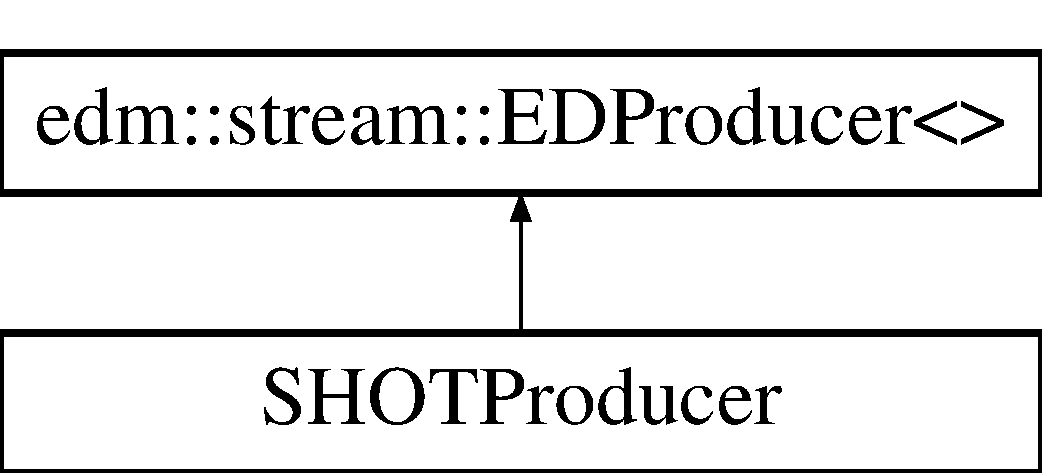
\includegraphics[height=2.000000cm]{classSHOTProducer}
\end{center}
\end{figure}
\subsection*{Public Member Functions}
\begin{DoxyCompactItemize}
\item 
\hypertarget{classSHOTProducer_a13653983741e35b0b7641672b25dec62}{{\bfseries S\-H\-O\-T\-Producer} (const edm\-::\-Parameter\-Set \&)}\label{classSHOTProducer_a13653983741e35b0b7641672b25dec62}

\end{DoxyCompactItemize}
\subsection*{Static Public Member Functions}
\begin{DoxyCompactItemize}
\item 
\hypertarget{classSHOTProducer_a2c8ce076825b6da1d56ad3fc51fbf55b}{static void {\bfseries fill\-Descriptions} (edm\-::\-Configuration\-Descriptions \&descriptions)}\label{classSHOTProducer_a2c8ce076825b6da1d56ad3fc51fbf55b}

\end{DoxyCompactItemize}


\subsection{Detailed Description}
Description\-: \mbox{[}one line class summary\mbox{]}

Implementation\-: \mbox{[}Notes on implementation\mbox{]} 

The documentation for this class was generated from the following file\-:\begin{DoxyCompactItemize}
\item 
/home/travis/build/susy2015/\-Top\-Tagger/\-Top\-Tagger/plugins/S\-H\-O\-T\-Producer.\-cc\end{DoxyCompactItemize}

\hypertarget{classcfg_1_1SimpleTerm}{\section{cfg\-:\-:Simple\-Term Class Reference}
\label{classcfg_1_1SimpleTerm}\index{cfg\-::\-Simple\-Term@{cfg\-::\-Simple\-Term}}
}
Inheritance diagram for cfg\-:\-:Simple\-Term\-:\begin{figure}[H]
\begin{center}
\leavevmode
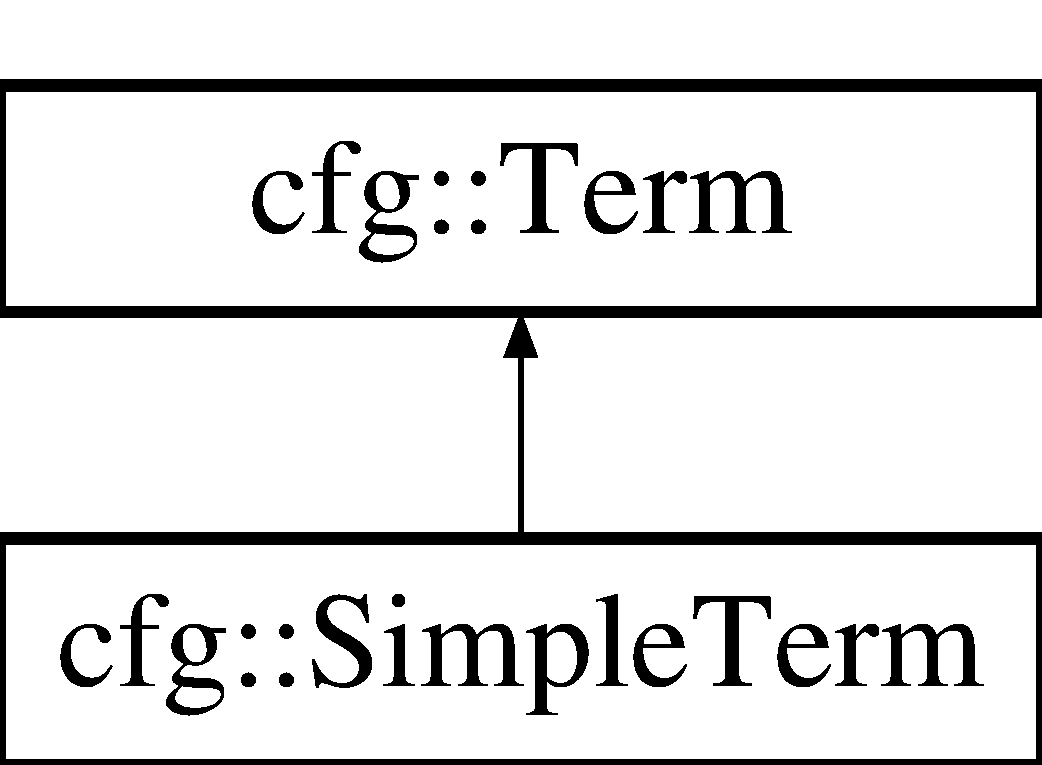
\includegraphics[height=2.000000cm]{classcfg_1_1SimpleTerm}
\end{center}
\end{figure}
\subsection*{Public Member Functions}
\begin{DoxyCompactItemize}
\item 
\hypertarget{classcfg_1_1SimpleTerm_a75fb72281bef8ed5836c9dcd2f7fbdc6}{{\bfseries Simple\-Term} (const std\-::string \&item\-Name, const std\-::string \&op, const \hyperlink{classcfg_1_1Literal}{Literal} \&value)}\label{classcfg_1_1SimpleTerm_a75fb72281bef8ed5836c9dcd2f7fbdc6}

\item 
\hypertarget{classcfg_1_1SimpleTerm_a339edfb7a0039617df99d96cf2d3ca76}{\hyperlink{classcfg_1_1SimpleTerm_a339edfb7a0039617df99d96cf2d3ca76}{Simple\-Term} (const std\-::string \&item\-Name, const std\-::string \&op, const std\-::vector$<$ \hyperlink{classcfg_1_1Literal}{Literal} $>$ \&value)}\label{classcfg_1_1SimpleTerm_a339edfb7a0039617df99d96cf2d3ca76}

\begin{DoxyCompactList}\small\item\em \char`\"{}\-I\-N\char`\"{} \end{DoxyCompactList}\item 
\hypertarget{classcfg_1_1SimpleTerm_a14ee322178830857278e9d1ae0f1cfa8}{virtual bool {\bfseries matches} (const \hyperlink{classcfg_1_1Context}{Context} \&cxt) const }\label{classcfg_1_1SimpleTerm_a14ee322178830857278e9d1ae0f1cfa8}

\item 
\hypertarget{classcfg_1_1SimpleTerm_a208a5ea6db041e9cae39946c914805e5}{virtual std\-::set$<$ std\-::string $>$ {\bfseries queried\-Items} () const }\label{classcfg_1_1SimpleTerm_a208a5ea6db041e9cae39946c914805e5}

\item 
\hypertarget{classcfg_1_1SimpleTerm_ab118b79bc95b7a1e22670ead1f352c89}{virtual std\-::ostream \& {\bfseries put} (std\-::ostream \&o) const }\label{classcfg_1_1SimpleTerm_ab118b79bc95b7a1e22670ead1f352c89}

\end{DoxyCompactItemize}


The documentation for this class was generated from the following files\-:\begin{DoxyCompactItemize}
\item 
/home/travis/build/susy2015/\-Top\-Tagger/\-Cfg\-Parser/include/Condition.\-hh\item 
/home/travis/build/susy2015/\-Top\-Tagger/\-Cfg\-Parser/src/Condition.\-cc\end{DoxyCompactItemize}

\hypertarget{classhcalcfg_1_1StartStates}{\section{hcalcfg\-:\-:Start\-States Class Reference}
\label{classhcalcfg_1_1StartStates}\index{hcalcfg\-::\-Start\-States@{hcalcfg\-::\-Start\-States}}
}
\subsection*{Public Member Functions}
\begin{DoxyCompactItemize}
\item 
\hypertarget{classhcalcfg_1_1StartStates_a64bf9a4476042f86c54bb77a9de6ac53}{void {\bfseries set} (int key, int val)}\label{classhcalcfg_1_1StartStates_a64bf9a4476042f86c54bb77a9de6ac53}

\item 
\hypertarget{classhcalcfg_1_1StartStates_a76c2847b9d374dbccdc3ee910a92bfdd}{int {\bfseries state} (int key)}\label{classhcalcfg_1_1StartStates_a76c2847b9d374dbccdc3ee910a92bfdd}

\end{DoxyCompactItemize}


The documentation for this class was generated from the following file\-:\begin{DoxyCompactItemize}
\item 
/home/travis/build/susy2015/\-Top\-Tagger/\-Cfg\-Parser/include/Scanner.\-h\end{DoxyCompactItemize}

\hypertarget{classsubmitBatch_1_1SubmitJobs}{\section{submit\-Batch.\-Submit\-Jobs Class Reference}
\label{classsubmitBatch_1_1SubmitJobs}\index{submit\-Batch.\-Submit\-Jobs@{submit\-Batch.\-Submit\-Jobs}}
}
\subsection*{Public Member Functions}
\begin{DoxyCompactItemize}
\item 
\hypertarget{classsubmitBatch_1_1SubmitJobs_a843ed65a4017b4af7cf04e0b21140933}{def {\bfseries \-\_\-\-\_\-init\-\_\-\-\_\-}}\label{classsubmitBatch_1_1SubmitJobs_a843ed65a4017b4af7cf04e0b21140933}

\item 
\hypertarget{classsubmitBatch_1_1SubmitJobs_a6a4ec898aeef0cea46bb18ff8c3f385d}{def {\bfseries create\-Job}}\label{classsubmitBatch_1_1SubmitJobs_a6a4ec898aeef0cea46bb18ff8c3f385d}

\item 
\hypertarget{classsubmitBatch_1_1SubmitJobs_ab412ebdf6ba64e5186c084220e87bd87}{def {\bfseries \-\_\-\-\_\-call\-\_\-\-\_\-}}\label{classsubmitBatch_1_1SubmitJobs_ab412ebdf6ba64e5186c084220e87bd87}

\item 
\hypertarget{classsubmitBatch_1_1SubmitJobs_abe5167df9140c659b9014c7a24cd1b51}{def {\bfseries submit\-Jobs}}\label{classsubmitBatch_1_1SubmitJobs_abe5167df9140c659b9014c7a24cd1b51}

\end{DoxyCompactItemize}
\subsection*{Public Attributes}
\begin{DoxyCompactItemize}
\item 
\hypertarget{classsubmitBatch_1_1SubmitJobs_aa75a76efda487ad51213e50f4117e216}{{\bfseries N\-G\-P\-U}}\label{classsubmitBatch_1_1SubmitJobs_aa75a76efda487ad51213e50f4117e216}

\item 
\hypertarget{classsubmitBatch_1_1SubmitJobs_a10fc4d33c8173a5f02e8a2b8eeb36a63}{{\bfseries workdir}}\label{classsubmitBatch_1_1SubmitJobs_a10fc4d33c8173a5f02e8a2b8eeb36a63}

\item 
\hypertarget{classsubmitBatch_1_1SubmitJobs_ab4cc17bbaefd9389d791a0f45a9acef7}{{\bfseries submit\-List}}\label{classsubmitBatch_1_1SubmitJobs_ab4cc17bbaefd9389d791a0f45a9acef7}

\item 
\hypertarget{classsubmitBatch_1_1SubmitJobs_ac2efb2678325fd2ab80c028dc7e5e784}{{\bfseries current\-G\-P\-U}}\label{classsubmitBatch_1_1SubmitJobs_ac2efb2678325fd2ab80c028dc7e5e784}

\end{DoxyCompactItemize}


The documentation for this class was generated from the following file\-:\begin{DoxyCompactItemize}
\item 
/home/travis/build/susy2015/\-Top\-Tagger/\-Tools/python/submit\-Batch.\-py\end{DoxyCompactItemize}

\hypertarget{classtaggerOptions_1_1taggerOptions}{\section{tagger\-Options.\-tagger\-Options Class Reference}
\label{classtaggerOptions_1_1taggerOptions}\index{tagger\-Options.\-tagger\-Options@{tagger\-Options.\-tagger\-Options}}
}


The documentation for this class was generated from the following file\-:\begin{DoxyCompactItemize}
\item 
/home/travis/build/susy2015/\-Top\-Tagger/\-Tools/python/tagger\-Options.\-py\end{DoxyCompactItemize}

\hypertarget{classcfg_1_1Term}{\section{cfg\-:\-:Term Class Reference}
\label{classcfg_1_1Term}\index{cfg\-::\-Term@{cfg\-::\-Term}}
}
Inheritance diagram for cfg\-:\-:Term\-:\begin{figure}[H]
\begin{center}
\leavevmode
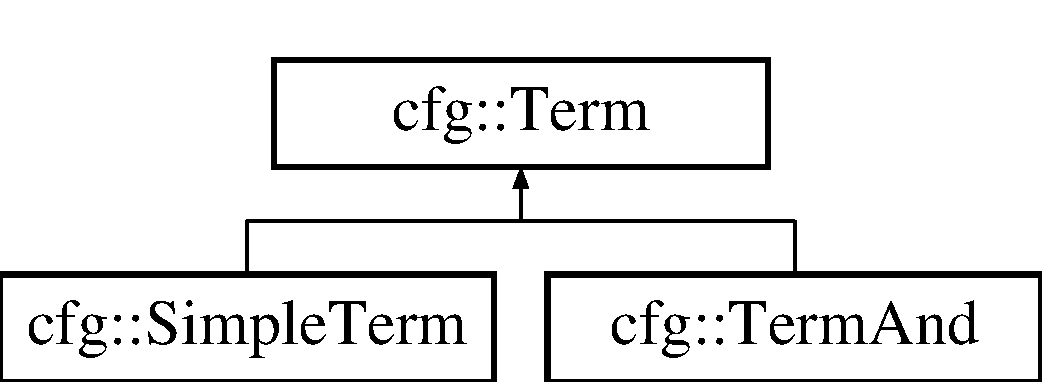
\includegraphics[height=2.000000cm]{classcfg_1_1Term}
\end{center}
\end{figure}
\subsection*{Public Member Functions}
\begin{DoxyCompactItemize}
\item 
\hypertarget{classcfg_1_1Term_a8cfe026d2155bfe41b41252a4bc12055}{virtual bool {\bfseries matches} (const \hyperlink{classcfg_1_1Context}{Context} \&cxt) const =0}\label{classcfg_1_1Term_a8cfe026d2155bfe41b41252a4bc12055}

\item 
\hypertarget{classcfg_1_1Term_af47c75ea82799805b7daafd789a86c6d}{virtual std\-::ostream \& {\bfseries put} (std\-::ostream \&o) const =0}\label{classcfg_1_1Term_af47c75ea82799805b7daafd789a86c6d}

\item 
\hypertarget{classcfg_1_1Term_a16d79489fd5a64500706f2ad98161bad}{virtual std\-::set$<$ std\-::string $>$ {\bfseries queried\-Items} () const =0}\label{classcfg_1_1Term_a16d79489fd5a64500706f2ad98161bad}

\end{DoxyCompactItemize}


The documentation for this class was generated from the following file\-:\begin{DoxyCompactItemize}
\item 
/home/travis/build/susy2015/\-Top\-Tagger/\-Cfg\-Parser/include/Condition.\-hh\end{DoxyCompactItemize}

\hypertarget{classcfg_1_1TermAnd}{\section{cfg\-:\-:Term\-And Class Reference}
\label{classcfg_1_1TermAnd}\index{cfg\-::\-Term\-And@{cfg\-::\-Term\-And}}
}
Inheritance diagram for cfg\-:\-:Term\-And\-:\begin{figure}[H]
\begin{center}
\leavevmode
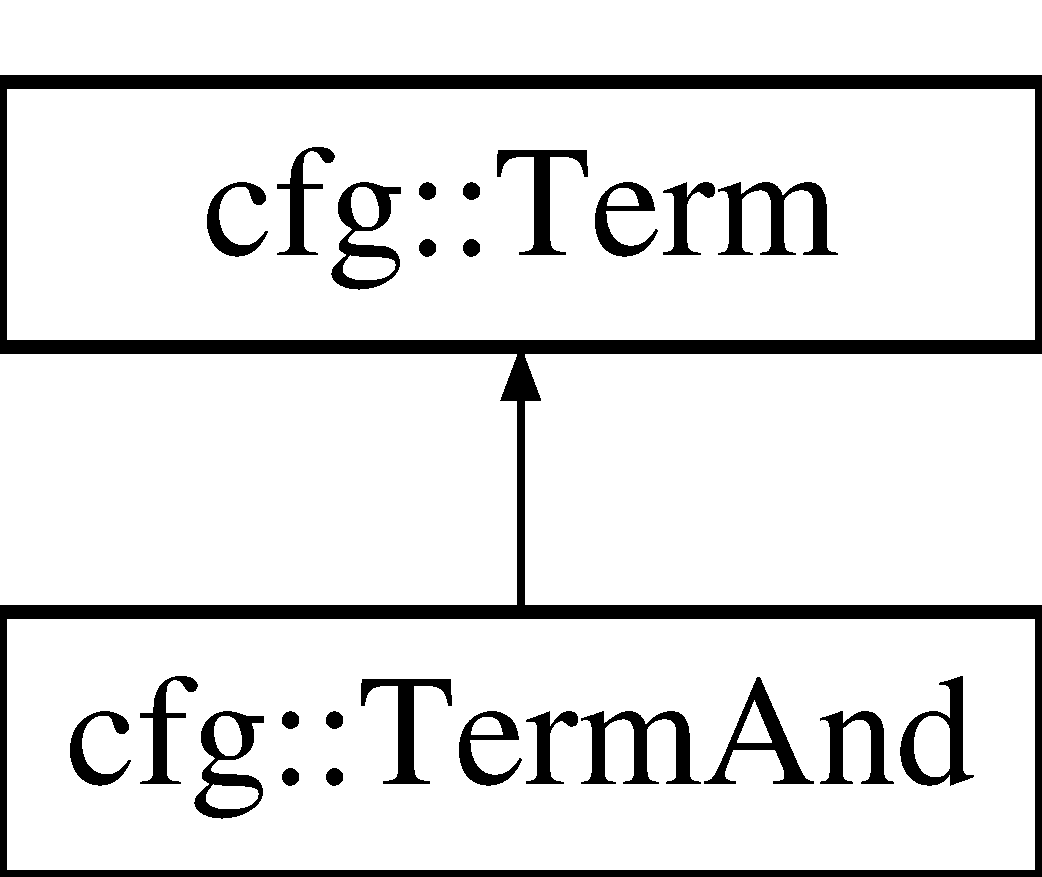
\includegraphics[height=2.000000cm]{classcfg_1_1TermAnd}
\end{center}
\end{figure}
\subsection*{Public Member Functions}
\begin{DoxyCompactItemize}
\item 
\hypertarget{classcfg_1_1TermAnd_af5918a76635aeca7bc01e5108f3206a1}{virtual bool {\bfseries matches} (const \hyperlink{classcfg_1_1Context}{Context} \&cxt) const }\label{classcfg_1_1TermAnd_af5918a76635aeca7bc01e5108f3206a1}

\item 
\hypertarget{classcfg_1_1TermAnd_a84dc305009d030accaef9600b9aaabb4}{void {\bfseries And} (\hyperlink{classcfg_1_1Term}{Term} $\ast$t)}\label{classcfg_1_1TermAnd_a84dc305009d030accaef9600b9aaabb4}

\item 
\hypertarget{classcfg_1_1TermAnd_a81179a1b7c8a4376702c4f8db261976c}{virtual std\-::set$<$ std\-::string $>$ {\bfseries queried\-Items} () const }\label{classcfg_1_1TermAnd_a81179a1b7c8a4376702c4f8db261976c}

\item 
\hypertarget{classcfg_1_1TermAnd_a612399f722085d523e5bdeac915182ca}{virtual std\-::ostream \& {\bfseries put} (std\-::ostream \&o) const }\label{classcfg_1_1TermAnd_a612399f722085d523e5bdeac915182ca}

\end{DoxyCompactItemize}


The documentation for this class was generated from the following files\-:\begin{DoxyCompactItemize}
\item 
/home/travis/build/susy2015/\-Top\-Tagger/\-Cfg\-Parser/include/Condition.\-hh\item 
/home/travis/build/susy2015/\-Top\-Tagger/\-Cfg\-Parser/src/Condition.\-cc\end{DoxyCompactItemize}

\hypertarget{classhcalcfg_1_1Token}{\section{hcalcfg\-:\-:Token Class Reference}
\label{classhcalcfg_1_1Token}\index{hcalcfg\-::\-Token@{hcalcfg\-::\-Token}}
}
\subsection*{Public Attributes}
\begin{DoxyCompactItemize}
\item 
\hypertarget{classhcalcfg_1_1Token_a161bdce3a4fdcb6a8f60bea7a90f59a4}{int {\bfseries kind}}\label{classhcalcfg_1_1Token_a161bdce3a4fdcb6a8f60bea7a90f59a4}

\item 
\hypertarget{classhcalcfg_1_1Token_a887ce5f48551400f3f93995ea562626f}{int {\bfseries pos}}\label{classhcalcfg_1_1Token_a887ce5f48551400f3f93995ea562626f}

\item 
\hypertarget{classhcalcfg_1_1Token_acc25802f5d681ac4d13e6353e5fc927b}{int {\bfseries char\-Pos}}\label{classhcalcfg_1_1Token_acc25802f5d681ac4d13e6353e5fc927b}

\item 
\hypertarget{classhcalcfg_1_1Token_a6e212446af50850c1970486e45e9021d}{int {\bfseries col}}\label{classhcalcfg_1_1Token_a6e212446af50850c1970486e45e9021d}

\item 
\hypertarget{classhcalcfg_1_1Token_a830def96a4ec29f5a4c6f552f47df895}{int {\bfseries line}}\label{classhcalcfg_1_1Token_a830def96a4ec29f5a4c6f552f47df895}

\item 
\hypertarget{classhcalcfg_1_1Token_a4f020a9e2e62374cc23f4543d2f0d96d}{wchar\-\_\-t $\ast$ {\bfseries val}}\label{classhcalcfg_1_1Token_a4f020a9e2e62374cc23f4543d2f0d96d}

\item 
\hypertarget{classhcalcfg_1_1Token_af869066be56489268d6c6a0e427a28e1}{\hyperlink{classhcalcfg_1_1Token}{Token} $\ast$ {\bfseries next}}\label{classhcalcfg_1_1Token_af869066be56489268d6c6a0e427a28e1}

\end{DoxyCompactItemize}


The documentation for this class was generated from the following files\-:\begin{DoxyCompactItemize}
\item 
/home/travis/build/susy2015/\-Top\-Tagger/\-Cfg\-Parser/include/Scanner.\-h\item 
/home/travis/build/susy2015/\-Top\-Tagger/\-Cfg\-Parser/src/Scanner.\-cpp\end{DoxyCompactItemize}

\hypertarget{classTopTagger_1_1Top}{\section{Top\-Tagger.\-Top Class Reference}
\label{classTopTagger_1_1Top}\index{Top\-Tagger.\-Top@{Top\-Tagger.\-Top}}
}
\subsection*{Public Member Functions}
\begin{DoxyCompactItemize}
\item 
\hypertarget{classTopTagger_1_1Top_abad89dad65df72031cf3adf48c182f34}{def {\bfseries \-\_\-\-\_\-init\-\_\-\-\_\-}}\label{classTopTagger_1_1Top_abad89dad65df72031cf3adf48c182f34}

\item 
\hypertarget{classTopTagger_1_1Top_a067729c8437c2ace6a974c62cf874a50}{def {\bfseries \-\_\-\-\_\-str\-\_\-\-\_\-}}\label{classTopTagger_1_1Top_a067729c8437c2ace6a974c62cf874a50}

\item 
\hypertarget{classTopTagger_1_1Top_acc9c36369f671d145e50950810485593}{def {\bfseries \-\_\-\-\_\-repr\-\_\-\-\_\-}}\label{classTopTagger_1_1Top_acc9c36369f671d145e50950810485593}

\end{DoxyCompactItemize}
\subsection*{Public Attributes}
\begin{DoxyCompactItemize}
\item 
\hypertarget{classTopTagger_1_1Top_a1eab0b54181fd0ea574e57b35ccc59e1}{{\bfseries pt}}\label{classTopTagger_1_1Top_a1eab0b54181fd0ea574e57b35ccc59e1}

\item 
\hypertarget{classTopTagger_1_1Top_a42895f21679a2a03ea4e320a9219b682}{{\bfseries eta}}\label{classTopTagger_1_1Top_a42895f21679a2a03ea4e320a9219b682}

\item 
\hypertarget{classTopTagger_1_1Top_af5ec16e9139fc919b6cca9f222915993}{{\bfseries phi}}\label{classTopTagger_1_1Top_af5ec16e9139fc919b6cca9f222915993}

\item 
\hypertarget{classTopTagger_1_1Top_a2a8d1553340a83f07989044d903813b2}{{\bfseries mass}}\label{classTopTagger_1_1Top_a2a8d1553340a83f07989044d903813b2}

\item 
\hypertarget{classTopTagger_1_1Top_a361f8b14fe698a10a815504bf554b5f9}{{\bfseries disc}}\label{classTopTagger_1_1Top_a361f8b14fe698a10a815504bf554b5f9}

\item 
\hypertarget{classTopTagger_1_1Top_a3da1fcb0f8ea21d672a105e30a03d496}{{\bfseries type}}\label{classTopTagger_1_1Top_a3da1fcb0f8ea21d672a105e30a03d496}

\item 
\hypertarget{classTopTagger_1_1Top_aebc3fb5ff67de0560cf769c4555de3b0}{{\bfseries j1\-Idx}}\label{classTopTagger_1_1Top_aebc3fb5ff67de0560cf769c4555de3b0}

\item 
\hypertarget{classTopTagger_1_1Top_a5543e5f414244684d33b9d0861013538}{{\bfseries j2\-Idx}}\label{classTopTagger_1_1Top_a5543e5f414244684d33b9d0861013538}

\item 
\hypertarget{classTopTagger_1_1Top_a71bca621aa593a25d15273386bda4cd0}{{\bfseries j3\-Idx}}\label{classTopTagger_1_1Top_a71bca621aa593a25d15273386bda4cd0}

\item 
\hypertarget{classTopTagger_1_1Top_a259645562ae12a67b9a3c5ea6a89264f}{{\bfseries sf}}\label{classTopTagger_1_1Top_a259645562ae12a67b9a3c5ea6a89264f}

\item 
\hypertarget{classTopTagger_1_1Top_a17325ceea5c3558fa47f96bd9a3eebb7}{{\bfseries systs}}\label{classTopTagger_1_1Top_a17325ceea5c3558fa47f96bd9a3eebb7}

\end{DoxyCompactItemize}


The documentation for this class was generated from the following file\-:\begin{DoxyCompactItemize}
\item 
/home/travis/build/susy2015/\-Top\-Tagger/\-Top\-Tagger/python/Top\-Tagger.\-py\end{DoxyCompactItemize}

\hypertarget{classTopCat}{\section{Top\-Cat Class Reference}
\label{classTopCat}\index{Top\-Cat@{Top\-Cat}}
}
\subsection*{Public Member Functions}
\begin{DoxyCompactItemize}
\item 
\hypertarget{classTopCat_a61e662422b74d9052978531013a119e8}{{\footnotesize template$<$typename T $>$ }\\bool {\bfseries Get\-Matched\-Top} (const std\-::vector$<$ T $>$ \&Top\-Cand, std\-::vector$<$ \hyperlink{classTopObject}{Top\-Object} $>$ \&Mached\-Top\-Cand, const std\-::vector$<$ T\-Lorentz\-Vector $>$ \&Gentop, std\-::vector$<$ T\-Lorentz\-Vector $>$ \&M\-Gentop)}\label{classTopCat_a61e662422b74d9052978531013a119e8}

\item 
\hypertarget{classTopCat_a179ae0049fa26f8bf1e651890cc996ac}{bool {\bfseries Get\-Matched\-Top} (std\-::vector$<$ T\-Lorentz\-Vector $>$ Top\-Cand, std\-::vector$<$ T\-Lorentz\-Vector $>$ \&Mached\-Top\-Cand, std\-::vector$<$ T\-Lorentz\-Vector $>$Gentop, std\-::vector$<$ T\-Lorentz\-Vector $>$ \&M\-Gentop)}\label{classTopCat_a179ae0049fa26f8bf1e651890cc996ac}

\item 
\hypertarget{classTopCat_a9b53819ee2fa66f3e6dd51e500c45670}{std\-::pair$<$ int, int $>$ {\bfseries Get\-Matched\-Top\-Const} (const std\-::vector$<$ \hyperlink{classConstituent}{Constituent} const $\ast$ $>$ \&topconst, const std\-::vector$<$ T\-Lorentz\-Vector $>$ \&gentopdau)}\label{classTopCat_a9b53819ee2fa66f3e6dd51e500c45670}

\item 
\hypertarget{classTopCat_acb1ae1bcd54353db3784447317f69dd5}{{\footnotesize template$<$typename T $>$ }\\std\-::pair$<$ std\-::vector$<$ int $>$\\*
, std\-::pair$<$ std\-::vector$<$ int $>$\\*
, std\-::vector$<$ T\-Lorentz\-Vector $>$ $>$ $>$ {\bfseries Top\-Const} (const std\-::vector$<$ T $>$ \&tops, const std\-::vector$<$ T\-Lorentz\-Vector $>$ \&gen\-Decay\-L\-Vec, const std\-::vector$<$ int $>$ \&gen\-Decay\-Pdg\-Id\-Vec, const std\-::vector$<$ int $>$ \&gen\-Decay\-Idx\-Vec, const std\-::vector$<$ int $>$ \&gen\-Decay\-Mom\-Idx\-Vec)}\label{classTopCat_acb1ae1bcd54353db3784447317f69dd5}

\end{DoxyCompactItemize}


The documentation for this class was generated from the following files\-:\begin{DoxyCompactItemize}
\item 
/home/travis/build/susy2015/\-Top\-Tagger/\-Tools/cpp/Tagger\-Utility.\-h\item 
/home/travis/build/susy2015/\-Top\-Tagger/\-Tools/cpp/Tagger\-Utility.\-cc\end{DoxyCompactItemize}

\hypertarget{classTopObject}{\section{Top\-Object Class Reference}
\label{classTopObject}\index{Top\-Object@{Top\-Object}}
}


{\ttfamily \#include $<$Top\-Object.\-h$>$}

\subsection*{Public Types}
\begin{DoxyCompactItemize}
\item 
enum \hyperlink{classTopObject_af82a20e421c29bc667af7cd73fc46ba4}{Type} \{ \\*
{\bfseries N\-O\-N\-E}, 
{\bfseries M\-E\-R\-G\-E\-D\-\_\-\-T\-O\-P}, 
{\bfseries S\-E\-M\-I\-M\-E\-R\-G\-E\-D\-W\-B\-\_\-\-T\-O\-P}, 
{\bfseries R\-E\-S\-O\-L\-V\-E\-D\-\_\-\-T\-O\-P}, 
\\*
{\bfseries M\-E\-R\-G\-E\-D\-\_\-\-W}, 
{\bfseries S\-E\-M\-I\-M\-E\-R\-G\-E\-D\-Q\-B\-\_\-\-T\-O\-P}, 
{\bfseries N\-T\-Y\-P\-E}, 
{\bfseries A\-N\-Y}
 \}
\end{DoxyCompactItemize}
\subsection*{Public Member Functions}
\begin{DoxyCompactItemize}
\item 
\hypertarget{classTopObject_a0eb6419f5a625d5ad777df5363e02f90}{\hyperlink{classTopObject_a0eb6419f5a625d5ad777df5363e02f90}{Top\-Object} ()}\label{classTopObject_a0eb6419f5a625d5ad777df5363e02f90}

\begin{DoxyCompactList}\small\item\em Construct default empty \hyperlink{classTopObject}{Top\-Object}. \end{DoxyCompactList}\item 
\hypertarget{classTopObject_a7888dbf304a6fb09af55b4a632cab5ef}{\hyperlink{classTopObject_a7888dbf304a6fb09af55b4a632cab5ef}{Top\-Object} (std\-::vector$<$ \hyperlink{classConstituent}{Constituent} const $\ast$ $>$ constituents, const \hyperlink{classTopObject_af82a20e421c29bc667af7cd73fc46ba4}{Type} \&type=N\-O\-N\-E)}\label{classTopObject_a7888dbf304a6fb09af55b4a632cab5ef}

\begin{DoxyCompactList}\small\item\em Construct a \hyperlink{classTopObject}{Top\-Object} from a vector of constituent jets. \end{DoxyCompactList}\item 
\hypertarget{classTopObject_adafc98b5660ac2ca92f9115668de2c10}{void \hyperlink{classTopObject_adafc98b5660ac2ca92f9115668de2c10}{add\-Constituent} (\hyperlink{classConstituent}{Constituent} const $\ast$constituent)}\label{classTopObject_adafc98b5660ac2ca92f9115668de2c10}

\begin{DoxyCompactList}\small\item\em Add a new constituent to the \hyperlink{classTopObject}{Top\-Object}. \end{DoxyCompactList}\item 
\hypertarget{classTopObject_abf5123e8c707e9059c8ec96b35643bef}{void \hyperlink{classTopObject_abf5123e8c707e9059c8ec96b35643bef}{set\-Discriminator} (const double disc)}\label{classTopObject_abf5123e8c707e9059c8ec96b35643bef}

\begin{DoxyCompactList}\small\item\em Set the Top discriminator for this candidate. \end{DoxyCompactList}\item 
\hypertarget{classTopObject_a52fbbf2a336d0e174f509304f8c1c984}{const T\-Lorentz\-Vector \& \hyperlink{classTopObject_a52fbbf2a336d0e174f509304f8c1c984}{p} () const }\label{classTopObject_a52fbbf2a336d0e174f509304f8c1c984}

\begin{DoxyCompactList}\small\item\em Returns the 4-\/vector momentum of the top candidate. \end{DoxyCompactList}\item 
\hypertarget{classTopObject_ac59c3a52925131b1ea7e5bf5c014aa2d}{const T\-Lorentz\-Vector \& \hyperlink{classTopObject_ac59c3a52925131b1ea7e5bf5c014aa2d}{P} () const }\label{classTopObject_ac59c3a52925131b1ea7e5bf5c014aa2d}

\begin{DoxyCompactList}\small\item\em Returns the 4-\/vector momentum of the top candidate. \end{DoxyCompactList}\item 
\hypertarget{classTopObject_ad6c8e1a0ef46d400075b1c2dbb05e37d}{double \hyperlink{classTopObject_ad6c8e1a0ef46d400075b1c2dbb05e37d}{get\-D\-Rmax} () const }\label{classTopObject_ad6c8e1a0ef46d400075b1c2dbb05e37d}

\begin{DoxyCompactList}\small\item\em Returns the maximum d\-R seperation between the overall top candidate and any of the individual constituents. \end{DoxyCompactList}\item 
\hypertarget{classTopObject_a6751962b83bc4b348cebee05aa23c299}{double \hyperlink{classTopObject_a6751962b83bc4b348cebee05aa23c299}{get\-D\-Theta\-Min} () const }\label{classTopObject_a6751962b83bc4b348cebee05aa23c299}

\begin{DoxyCompactList}\small\item\em Returns the minimum angular seperation between the top candidate and any of the individual constituents. \end{DoxyCompactList}\item 
\hypertarget{classTopObject_afd9525b26ff81392af3773c5c88f2f68}{double \hyperlink{classTopObject_afd9525b26ff81392af3773c5c88f2f68}{get\-D\-Theta\-Max} () const }\label{classTopObject_afd9525b26ff81392af3773c5c88f2f68}

\begin{DoxyCompactList}\small\item\em Returns the maximum angular seperation between the top candidate and any of the individual constituents. \end{DoxyCompactList}\item 
\hypertarget{classTopObject_a144b61f5139eb1bef7bc00cee17deaf7}{double \hyperlink{classTopObject_a144b61f5139eb1bef7bc00cee17deaf7}{get\-Discriminator} () const }\label{classTopObject_a144b61f5139eb1bef7bc00cee17deaf7}

\begin{DoxyCompactList}\small\item\em Returns the top discriminator for this candidate. \end{DoxyCompactList}\item 
\hypertarget{classTopObject_a74f6fdda7a11b18b599c4a37294d26b9}{\hyperlink{classTopObject_af82a20e421c29bc667af7cd73fc46ba4}{Type} \hyperlink{classTopObject_a74f6fdda7a11b18b599c4a37294d26b9}{get\-Type} () const }\label{classTopObject_a74f6fdda7a11b18b599c4a37294d26b9}

\begin{DoxyCompactList}\small\item\em Returnes the type of top. \end{DoxyCompactList}\item 
\hypertarget{classTopObject_a3bd54d089da20318d1733c2d4e28493a}{const std\-::vector$<$ \hyperlink{classConstituent}{Constituent} \\*
const $\ast$ $>$ \& \hyperlink{classTopObject_a3bd54d089da20318d1733c2d4e28493a}{get\-Constituents} () const }\label{classTopObject_a3bd54d089da20318d1733c2d4e28493a}

\begin{DoxyCompactList}\small\item\em Returns the internal vector of constituents which are used to construct the \hyperlink{classTopObject}{Top\-Object}. \end{DoxyCompactList}\item 
\hypertarget{classTopObject_a562bafee171bf66c283d519c8021672d}{int \hyperlink{classTopObject_a562bafee171bf66c283d519c8021672d}{get\-N\-Constituents} () const }\label{classTopObject_a562bafee171bf66c283d519c8021672d}

\begin{DoxyCompactList}\small\item\em The number of constituents in this \hyperlink{classTopObject}{Top\-Object}. \end{DoxyCompactList}\item 
\hypertarget{classTopObject_a2b5bb6b014c80262b748171698ba1042}{int \hyperlink{classTopObject_a2b5bb6b014c80262b748171698ba1042}{get\-N\-B\-Constituents} (double cvs\-Cut, double eta\-Cut=2.\-4) const }\label{classTopObject_a2b5bb6b014c80262b748171698ba1042}

\begin{DoxyCompactList}\small\item\em The number of b-\/tagged constituents based on the b-\/tagging discriminator cut and the jet eta. \end{DoxyCompactList}\item 
\hypertarget{classTopObject_a51cc6fbaacb2cf502cad0b57d99ae91f}{decltype(gen\-Match\-Possibilities\-\_\-) \\*
const \& \hyperlink{classTopObject_a51cc6fbaacb2cf502cad0b57d99ae91f}{get\-Gen\-Top\-Matches} () const }\label{classTopObject_a51cc6fbaacb2cf502cad0b57d99ae91f}

\begin{DoxyCompactList}\small\item\em Returns the list of all possible generator level tops which could be a match to the \hyperlink{classTopObject}{Top\-Object}. This requires that generator level information is passed to the top tagger. \end{DoxyCompactList}\item 
\hypertarget{classTopObject_a80c459ce3d60d1402087ceead3999e45}{const T\-Lorentz\-Vector $\ast$ \hyperlink{classTopObject_a80c459ce3d60d1402087ceead3999e45}{get\-Best\-Gen\-Top\-Match} (const double d\-R\-Max=0.\-6) const }\label{classTopObject_a80c459ce3d60d1402087ceead3999e45}

\begin{DoxyCompactList}\small\item\em Returns the best matched genrator level top based on the possible matches based on the parameter d\-R\-Max which defines the matching cone between the overall generator top and the top candidate. \end{DoxyCompactList}\item 
\hypertarget{classTopObject_a77edcc1258a253b60747eb557c12dd52}{double \hyperlink{classTopObject_a77edcc1258a253b60747eb557c12dd52}{get\-M\-C\-Scale\-Factor} () const }\label{classTopObject_a77edcc1258a253b60747eb557c12dd52}

\begin{DoxyCompactList}\small\item\em Return the scale factor used to scale simulation events so that they better match data. \end{DoxyCompactList}\item 
\hypertarget{classTopObject_add523f130ec310825913f90f2ad92cd1}{double \hyperlink{classTopObject_add523f130ec310825913f90f2ad92cd1}{get\-Systematic\-Uncertainty} (const std\-::string \&source) const }\label{classTopObject_add523f130ec310825913f90f2ad92cd1}

\begin{DoxyCompactList}\small\item\em Return systematic uncertainty. \end{DoxyCompactList}\end{DoxyCompactItemize}


\subsection{Detailed Description}
Container class which represents a top candidate or final selected top object. 

\subsection{Member Enumeration Documentation}
\hypertarget{classTopObject_af82a20e421c29bc667af7cd73fc46ba4}{\index{Top\-Object@{Top\-Object}!Type@{Type}}
\index{Type@{Type}!TopObject@{Top\-Object}}
\subsubsection[{Type}]{\setlength{\rightskip}{0pt plus 5cm}enum {\bf Top\-Object\-::\-Type}}}\label{classTopObject_af82a20e421c29bc667af7cd73fc46ba4}
Enum to select what flavor of object this \hyperlink{classTopObject}{Top\-Object} is. 

The documentation for this class was generated from the following files\-:\begin{DoxyCompactItemize}
\item 
/home/travis/build/susy2015/\-Top\-Tagger/\-Top\-Tagger/include/Top\-Object.\-h\item 
/home/travis/build/susy2015/\-Top\-Tagger/\-Top\-Tagger/src/Top\-Object.\-cpp\end{DoxyCompactItemize}

\hypertarget{classTopObjLite}{\section{Top\-Obj\-Lite Class Reference}
\label{classTopObjLite}\index{Top\-Obj\-Lite@{Top\-Obj\-Lite}}
}


{\ttfamily \#include $<$Top\-Obj\-Lite.\-h$>$}

Inheritance diagram for Top\-Obj\-Lite\-:\begin{figure}[H]
\begin{center}
\leavevmode
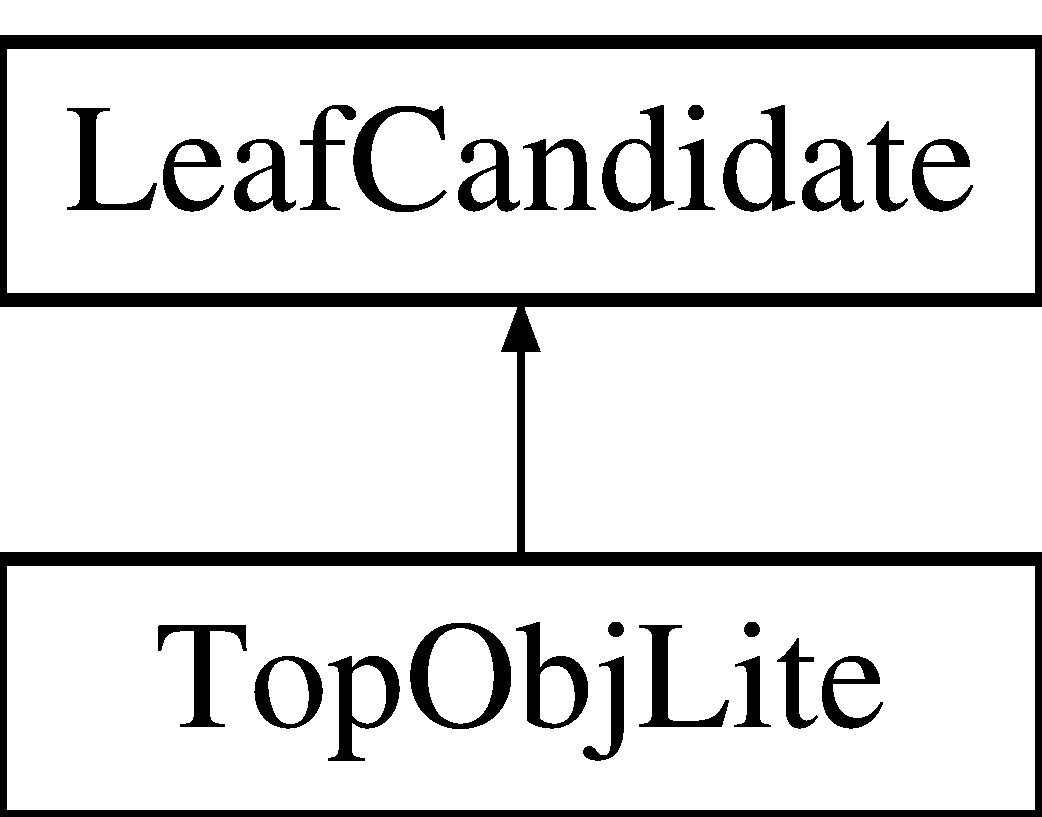
\includegraphics[height=2.000000cm]{classTopObjLite}
\end{center}
\end{figure}
\subsection*{Public Member Functions}
\begin{DoxyCompactItemize}
\item 
\hypertarget{classTopObjLite_a1cf0c97f077cbb9155d0de9a9d4df4b9}{{\bfseries Top\-Obj\-Lite} (const \hyperlink{classTopObject}{Top\-Object} \&top)}\label{classTopObjLite_a1cf0c97f077cbb9155d0de9a9d4df4b9}

\item 
\hypertarget{classTopObjLite_a9e634371b0ae7954bc946ecbff14e754}{float {\bfseries get\-Discriminator} () const }\label{classTopObjLite_a9e634371b0ae7954bc946ecbff14e754}

\item 
\hypertarget{classTopObjLite_aa360e450bcd7dff271051bb28c1ed415}{int {\bfseries get\-Type} () const }\label{classTopObjLite_aa360e450bcd7dff271051bb28c1ed415}

\item 
\hypertarget{classTopObjLite_ae370054eafb907b958fb5856a6fc54e9}{int {\bfseries get\-J1\-Idx} () const }\label{classTopObjLite_ae370054eafb907b958fb5856a6fc54e9}

\item 
\hypertarget{classTopObjLite_aae4eed76d9d315bc6a78b13d47ac63b4}{int {\bfseries get\-J2\-Idx} () const }\label{classTopObjLite_aae4eed76d9d315bc6a78b13d47ac63b4}

\item 
\hypertarget{classTopObjLite_a421262844777ac8907942bec45b12d88}{int {\bfseries get\-J3\-Idx} () const }\label{classTopObjLite_a421262844777ac8907942bec45b12d88}

\end{DoxyCompactItemize}


\subsection{Detailed Description}
\hyperlink{classTopObjLite}{Top\-Obj\-Lite} is a version of top object which is derived from cmssw reco\-::\-Candidate (through reco\-::\-Leaf\-Candidate) to allow the critical information to be saved into nano\-A\-O\-D data format 

The documentation for this class was generated from the following file\-:\begin{DoxyCompactItemize}
\item 
/home/travis/build/susy2015/\-Top\-Tagger/\-Top\-Tagger/interface/Top\-Obj\-Lite.\-h\end{DoxyCompactItemize}

\hypertarget{classTopTagger}{\section{Top\-Tagger Class Reference}
\label{classTopTagger}\index{Top\-Tagger@{Top\-Tagger}}
}


{\ttfamily \#include $<$Top\-Tagger.\-h$>$}

\subsection*{Classes}
\begin{DoxyCompactItemize}
\item 
class \hyperlink{classTopTagger_1_1Top}{Top}
\item 
class \hyperlink{classTopTagger_1_1TopTagger}{Top\-Tagger}
\item 
class \hyperlink{classTopTagger_1_1TopTaggerResult}{Top\-Tagger\-Result}
\end{DoxyCompactItemize}
\subsection*{Public Member Functions}
\begin{DoxyCompactItemize}
\item 
\hypertarget{classTopTagger_a26e4654b1eef1f7e7dcffeb02b9fc41b}{\hyperlink{classTopTagger_a26e4654b1eef1f7e7dcffeb02b9fc41b}{Top\-Tagger} ()}\label{classTopTagger_a26e4654b1eef1f7e7dcffeb02b9fc41b}

\begin{DoxyCompactList}\small\item\em Default constructor to create an empty \hyperlink{classTopTagger}{Top\-Tagger} object. \end{DoxyCompactList}\item 
\hypertarget{classTopTagger_a21e38d6b697bc079ab6fb0eb7a1ea3bb}{\hyperlink{classTopTagger_a21e38d6b697bc079ab6fb0eb7a1ea3bb}{Top\-Tagger} (const std\-::string \&cfg\-File\-Name, const std\-::string \&working\-Dir)}\label{classTopTagger_a21e38d6b697bc079ab6fb0eb7a1ea3bb}

\begin{DoxyCompactList}\small\item\em Constructor to initialize \hyperlink{classTopTagger}{Top\-Tagger} object from the provided configuration file. \end{DoxyCompactList}\item 
void \hyperlink{classTopTagger_ad7e22571559cb7afe0f0cf0e14d1ef41}{set\-Verbosity} (const int verbosity)
\item 
void \hyperlink{classTopTagger_ae117c09fc42674a09247fd1ad8dcb3ce}{set\-Rethrow} (const bool re\-Throw)
\item 
void \hyperlink{classTopTagger_ae03dce4873628bfd529924a9004b3304}{set\-Working\-Directory} (const std\-::string \&working\-Directory)
\item 
void \hyperlink{classTopTagger_ac18bfe0673dbd05973f45c668ed2b190}{set\-Cfg\-File} (const std\-::string \&)
\item 
void \hyperlink{classTopTagger_ae7a38be12023643495adea6f9a696ff3}{set\-Cfg\-File\-Direct} (const std\-::string \&)
\item 
void \hyperlink{classTopTagger_accf43da3b1469e524bfe6f568116219a}{run\-Tagger} (const std\-::vector$<$ \hyperlink{classConstituent}{Constituent} $>$ \&)
\item 
void \hyperlink{classTopTagger_ac4d5c2b7983a99495fa6cfa7e0287e74}{run\-Tagger} (std\-::vector$<$ \hyperlink{classConstituent}{Constituent} $>$ \&\&)
\item 
const \hyperlink{classTopTaggerResults}{Top\-Tagger\-Results} \& \hyperlink{classTopTagger_ac6f06aeb683b0b761ad09ac018e11d08}{get\-Results} () const 
\end{DoxyCompactItemize}
\subsection*{Public Attributes}
\begin{DoxyCompactItemize}
\item 
\hypertarget{classTopTagger_a482c3ca721ab70156011038be1ab88b8}{tuple {\bfseries parser} = optparse.\-Option\-Parser()}\label{classTopTagger_a482c3ca721ab70156011038be1ab88b8}

\item 
\hypertarget{classTopTagger_a9439149c855b5990c2b8382f56881720}{tuple {\bfseries f} = R\-O\-O\-T.\-T\-File.\-Open(options.\-input\-File)}\label{classTopTagger_a9439149c855b5990c2b8382f56881720}

\item 
\hypertarget{classTopTagger_adb9ad8b9c2a2261fc433b96f8adcb5cb}{tuple {\bfseries tree} = f.\-Get(options.\-tree\-Name)}\label{classTopTagger_adb9ad8b9c2a2261fc433b96f8adcb5cb}

\item 
\hypertarget{classTopTagger_a8f479f6e3e86c29ffe18b45eaf87b680}{tuple {\bfseries tt} = \hyperlink{classTopTagger_1_1TopTagger}{Top\-Tagger}(options.\-tagger\-Cfg, options.\-work\-Dir)}\label{classTopTagger_a8f479f6e3e86c29ffe18b45eaf87b680}

\item 
\hypertarget{classTopTagger_a5fe6daaea9a504350d3c1c33dd87e94d}{tuple {\bfseries tops} = get\-Tops\-From\-Example\-File(tt, event)}\label{classTopTagger_a5fe6daaea9a504350d3c1c33dd87e94d}

\end{DoxyCompactItemize}


\subsection{Detailed Description}
This class holds the primary structure of the tagger. It is responsible for parsing the configuration file for the tagger, instantiating and running the requested modules, and storing the common results objects for the modules and user.

The \hyperlink{classTopTagger}{Top\-Tagger} module is the primary (and only mandatory) section in every top tagger configuration. This section defines all the other top tagger modules which will be run and in which order. This module has 2 variables (both arrays) Which are used to define the module run order and if necessary the module context name. 
\begin{DoxyParams}{Parameters}
{\em module\mbox{[}$\,$\mbox{]}} & (string) This variable is an array and is used to define which other modules will be run and in which order. This can be any module listed here in this section. \\
\hline
{\em context\mbox{[}$\,$\mbox{]}} & (string) This variable must be specified for any module being run more than once to specify what context name to read its configuration from. \\
\hline
\end{DoxyParams}


\subsection{Member Function Documentation}
\hypertarget{classTopTagger_ac6f06aeb683b0b761ad09ac018e11d08}{\index{Top\-Tagger@{Top\-Tagger}!get\-Results@{get\-Results}}
\index{get\-Results@{get\-Results}!TopTagger@{Top\-Tagger}}
\subsubsection[{get\-Results}]{\setlength{\rightskip}{0pt plus 5cm}const {\bf Top\-Tagger\-Results} \& Top\-Tagger\-::get\-Results (
\begin{DoxyParamCaption}
{}
\end{DoxyParamCaption}
) const}}\label{classTopTagger_ac6f06aeb683b0b761ad09ac018e11d08}
Gets the top tagger results object from the external user. Results are returned as a const reference to a \hyperlink{classTopTaggerResults}{Top\-Tagger\-Results} object. \hypertarget{classTopTagger_accf43da3b1469e524bfe6f568116219a}{\index{Top\-Tagger@{Top\-Tagger}!run\-Tagger@{run\-Tagger}}
\index{run\-Tagger@{run\-Tagger}!TopTagger@{Top\-Tagger}}
\subsubsection[{run\-Tagger}]{\setlength{\rightskip}{0pt plus 5cm}void Top\-Tagger\-::run\-Tagger (
\begin{DoxyParamCaption}
\item[{const std\-::vector$<$ {\bf Constituent} $>$ \&}]{constituents}
\end{DoxyParamCaption}
)}}\label{classTopTagger_accf43da3b1469e524bfe6f568116219a}
Runs the top tagger modules specified in the configuration file. Run once per event. \hypertarget{classTopTagger_ac4d5c2b7983a99495fa6cfa7e0287e74}{\index{Top\-Tagger@{Top\-Tagger}!run\-Tagger@{run\-Tagger}}
\index{run\-Tagger@{run\-Tagger}!TopTagger@{Top\-Tagger}}
\subsubsection[{run\-Tagger}]{\setlength{\rightskip}{0pt plus 5cm}void Top\-Tagger\-::run\-Tagger (
\begin{DoxyParamCaption}
\item[{std\-::vector$<$ {\bf Constituent} $>$ \&\&}]{constituents}
\end{DoxyParamCaption}
)}}\label{classTopTagger_ac4d5c2b7983a99495fa6cfa7e0287e74}
Runs the top tagger modules specified in the configuration file. Run once per event. \hypertarget{classTopTagger_ac18bfe0673dbd05973f45c668ed2b190}{\index{Top\-Tagger@{Top\-Tagger}!set\-Cfg\-File@{set\-Cfg\-File}}
\index{set\-Cfg\-File@{set\-Cfg\-File}!TopTagger@{Top\-Tagger}}
\subsubsection[{set\-Cfg\-File}]{\setlength{\rightskip}{0pt plus 5cm}void Top\-Tagger\-::set\-Cfg\-File (
\begin{DoxyParamCaption}
\item[{const std\-::string \&}]{cfg\-File\-Name}
\end{DoxyParamCaption}
)}}\label{classTopTagger_ac18bfe0673dbd05973f45c668ed2b190}
Set the configuration file to use to configure the \hyperlink{classTopTagger}{Top\-Tagger} object. This function expects the path to an external configuration file. \hypertarget{classTopTagger_ae7a38be12023643495adea6f9a696ff3}{\index{Top\-Tagger@{Top\-Tagger}!set\-Cfg\-File\-Direct@{set\-Cfg\-File\-Direct}}
\index{set\-Cfg\-File\-Direct@{set\-Cfg\-File\-Direct}!TopTagger@{Top\-Tagger}}
\subsubsection[{set\-Cfg\-File\-Direct}]{\setlength{\rightskip}{0pt plus 5cm}void Top\-Tagger\-::set\-Cfg\-File\-Direct (
\begin{DoxyParamCaption}
\item[{const std\-::string \&}]{cfg\-Text}
\end{DoxyParamCaption}
)}}\label{classTopTagger_ae7a38be12023643495adea6f9a696ff3}
Set the configuration file directly from a string. This function expects the configuration in the format of a raw string. \hypertarget{classTopTagger_ae117c09fc42674a09247fd1ad8dcb3ce}{\index{Top\-Tagger@{Top\-Tagger}!set\-Rethrow@{set\-Rethrow}}
\index{set\-Rethrow@{set\-Rethrow}!TopTagger@{Top\-Tagger}}
\subsubsection[{set\-Rethrow}]{\setlength{\rightskip}{0pt plus 5cm}void Top\-Tagger\-::set\-Rethrow (
\begin{DoxyParamCaption}
\item[{const bool}]{re\-Throw}
\end{DoxyParamCaption}
)\hspace{0.3cm}{\ttfamily [inline]}}}\label{classTopTagger_ae117c09fc42674a09247fd1ad8dcb3ce}
If set to true the \hyperlink{classTopTagger}{Top\-Tagger} internal error handeling will rethrow T\-T\-Exceptions, otherwise the exceptions will be handled internally. \hypertarget{classTopTagger_ad7e22571559cb7afe0f0cf0e14d1ef41}{\index{Top\-Tagger@{Top\-Tagger}!set\-Verbosity@{set\-Verbosity}}
\index{set\-Verbosity@{set\-Verbosity}!TopTagger@{Top\-Tagger}}
\subsubsection[{set\-Verbosity}]{\setlength{\rightskip}{0pt plus 5cm}void Top\-Tagger\-::set\-Verbosity (
\begin{DoxyParamCaption}
\item[{const int}]{verbosity}
\end{DoxyParamCaption}
)\hspace{0.3cm}{\ttfamily [inline]}}}\label{classTopTagger_ad7e22571559cb7afe0f0cf0e14d1ef41}
Set the verbosity level of the top tagger \par
 0 -\/ print nothing \par
 1 -\/ print exception error messages \hypertarget{classTopTagger_ae03dce4873628bfd529924a9004b3304}{\index{Top\-Tagger@{Top\-Tagger}!set\-Working\-Directory@{set\-Working\-Directory}}
\index{set\-Working\-Directory@{set\-Working\-Directory}!TopTagger@{Top\-Tagger}}
\subsubsection[{set\-Working\-Directory}]{\setlength{\rightskip}{0pt plus 5cm}void Top\-Tagger\-::set\-Working\-Directory (
\begin{DoxyParamCaption}
\item[{const std\-::string \&}]{working\-Directory}
\end{DoxyParamCaption}
)\hspace{0.3cm}{\ttfamily [inline]}}}\label{classTopTagger_ae03dce4873628bfd529924a9004b3304}
If set, the top tagger will look in this directory for cfg files. This must be called B\-E\-F\-O\-R\-E set\-Cfg\-File. 

The documentation for this class was generated from the following files\-:\begin{DoxyCompactItemize}
\item 
/home/travis/build/susy2015/\-Top\-Tagger/\-Top\-Tagger/interface/Top\-Tagger.\-h\item 
/home/travis/build/susy2015/\-Top\-Tagger/\-Top\-Tagger/python/Top\-Tagger.\-py\item 
/home/travis/build/susy2015/\-Top\-Tagger/\-Top\-Tagger/src/Top\-Tagger.\-cpp\end{DoxyCompactItemize}

\hypertarget{classTopTagger_1_1TopTagger}{\section{Top\-Tagger.\-Top\-Tagger Class Reference}
\label{classTopTagger_1_1TopTagger}\index{Top\-Tagger.\-Top\-Tagger@{Top\-Tagger.\-Top\-Tagger}}
}
\subsection*{Public Member Functions}
\begin{DoxyCompactItemize}
\item 
\hypertarget{classTopTagger_1_1TopTagger_a161704f0abdbd30d84f9cbae3e6a3336}{def {\bfseries \-\_\-\-\_\-init\-\_\-\-\_\-}}\label{classTopTagger_1_1TopTagger_a161704f0abdbd30d84f9cbae3e6a3336}

\item 
\hypertarget{classTopTagger_1_1TopTagger_a01b9ce257815a42bf961804c02af4af4}{def {\bfseries \-\_\-\-\_\-enter\-\_\-\-\_\-}}\label{classTopTagger_1_1TopTagger_a01b9ce257815a42bf961804c02af4af4}

\item 
\hypertarget{classTopTagger_1_1TopTagger_a2397ccfb8f06a6313e40428920a52c1d}{def {\bfseries \-\_\-\-\_\-del\-\_\-\-\_\-}}\label{classTopTagger_1_1TopTagger_a2397ccfb8f06a6313e40428920a52c1d}

\item 
\hypertarget{classTopTagger_1_1TopTagger_a2eb507c390722239ff1896e29fc7ccfd}{def {\bfseries \-\_\-\-\_\-exit\-\_\-\-\_\-}}\label{classTopTagger_1_1TopTagger_a2eb507c390722239ff1896e29fc7ccfd}

\item 
\hypertarget{classTopTagger_1_1TopTagger_abc0aaa0982639e8b221c44326092771c}{def {\bfseries initialize}}\label{classTopTagger_1_1TopTagger_abc0aaa0982639e8b221c44326092771c}

\item 
\hypertarget{classTopTagger_1_1TopTagger_a0a0d4427b64669028e10aa40bff98582}{def {\bfseries close}}\label{classTopTagger_1_1TopTagger_a0a0d4427b64669028e10aa40bff98582}

\item 
\hypertarget{classTopTagger_1_1TopTagger_a44a4d842cfa4823f0c675fde9c7919cb}{def {\bfseries run}}\label{classTopTagger_1_1TopTagger_a44a4d842cfa4823f0c675fde9c7919cb}

\item 
\hypertarget{classTopTagger_1_1TopTagger_a2bd7fb2e34eaf765f87bf3b9d27aecba}{def {\bfseries run\-From\-Nano\-A\-O\-D}}\label{classTopTagger_1_1TopTagger_a2bd7fb2e34eaf765f87bf3b9d27aecba}

\end{DoxyCompactItemize}
\subsection*{Public Attributes}
\begin{DoxyCompactItemize}
\item 
\hypertarget{classTopTagger_1_1TopTagger_af45e65fc54f3253625c2acc07f6f5db9}{{\bfseries cfg\-File}}\label{classTopTagger_1_1TopTagger_af45e65fc54f3253625c2acc07f6f5db9}

\item 
\hypertarget{classTopTagger_1_1TopTagger_aa7493aff4f860df39acfed315f4bb90b}{{\bfseries working\-Dir}}\label{classTopTagger_1_1TopTagger_aa7493aff4f860df39acfed315f4bb90b}

\item 
\hypertarget{classTopTagger_1_1TopTagger_ad62b10aba9cc9bdb06e94f3f106a9c0f}{{\bfseries first\-Event}}\label{classTopTagger_1_1TopTagger_ad62b10aba9cc9bdb06e94f3f106a9c0f}

\item 
\hypertarget{classTopTagger_1_1TopTagger_a400625b5e024d460bcef5109a4091241}{{\bfseries tt}}\label{classTopTagger_1_1TopTagger_a400625b5e024d460bcef5109a4091241}

\end{DoxyCompactItemize}


The documentation for this class was generated from the following file\-:\begin{DoxyCompactItemize}
\item 
/home/travis/build/susy2015/\-Top\-Tagger/\-Top\-Tagger/python/Top\-Tagger.\-py\end{DoxyCompactItemize}

\hypertarget{classTopTaggerProducer_1_1TopTaggerProducer}{\section{Top\-Tagger\-Producer.\-Top\-Tagger\-Producer Class Reference}
\label{classTopTaggerProducer_1_1TopTaggerProducer}\index{Top\-Tagger\-Producer.\-Top\-Tagger\-Producer@{Top\-Tagger\-Producer.\-Top\-Tagger\-Producer}}
}
Inheritance diagram for Top\-Tagger\-Producer.\-Top\-Tagger\-Producer\-:\begin{figure}[H]
\begin{center}
\leavevmode
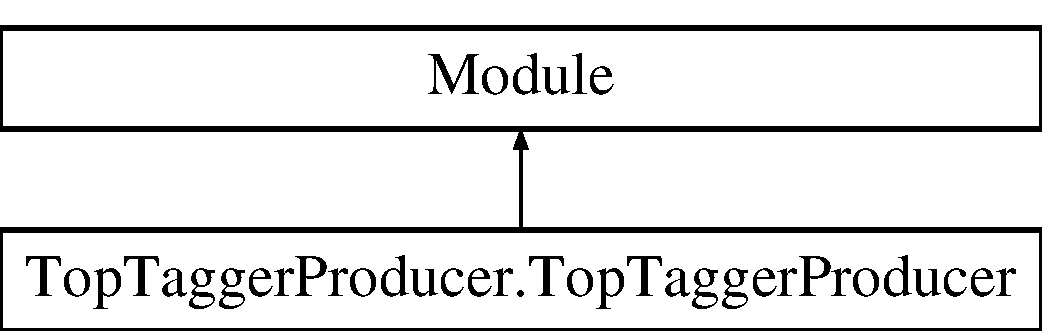
\includegraphics[height=2.000000cm]{classTopTaggerProducer_1_1TopTaggerProducer}
\end{center}
\end{figure}
\subsection*{Public Member Functions}
\begin{DoxyCompactItemize}
\item 
\hypertarget{classTopTaggerProducer_1_1TopTaggerProducer_a5c8f092651954386327e012eba734d20}{def {\bfseries \-\_\-\-\_\-init\-\_\-\-\_\-}}\label{classTopTaggerProducer_1_1TopTaggerProducer_a5c8f092651954386327e012eba734d20}

\item 
\hypertarget{classTopTaggerProducer_1_1TopTaggerProducer_a1d546bc8b364f136ac702cf1c784bb4f}{def {\bfseries begin\-Job}}\label{classTopTaggerProducer_1_1TopTaggerProducer_a1d546bc8b364f136ac702cf1c784bb4f}

\item 
\hypertarget{classTopTaggerProducer_1_1TopTaggerProducer_a79fe99bc2c04b09cc1a5ef9ed4aa7cc2}{def {\bfseries end\-Job}}\label{classTopTaggerProducer_1_1TopTaggerProducer_a79fe99bc2c04b09cc1a5ef9ed4aa7cc2}

\item 
\hypertarget{classTopTaggerProducer_1_1TopTaggerProducer_ab9a0f96420760a8ccd8ec514b9fbe0db}{def {\bfseries begin\-File}}\label{classTopTaggerProducer_1_1TopTaggerProducer_ab9a0f96420760a8ccd8ec514b9fbe0db}

\item 
\hypertarget{classTopTaggerProducer_1_1TopTaggerProducer_a039e05fd9e1ba5b350f58d92d4bdb77d}{def {\bfseries end\-File}}\label{classTopTaggerProducer_1_1TopTaggerProducer_a039e05fd9e1ba5b350f58d92d4bdb77d}

\item 
\hypertarget{classTopTaggerProducer_1_1TopTaggerProducer_aaaf76a9fb47e396d3028f1ef0fc44c9f}{def {\bfseries run\-From\-Nano\-A\-O\-D}}\label{classTopTaggerProducer_1_1TopTaggerProducer_aaaf76a9fb47e396d3028f1ef0fc44c9f}

\item 
def \hyperlink{classTopTaggerProducer_1_1TopTaggerProducer_a61f541cf9fa6fe2c85bef6f35d388b53}{analyze}
\end{DoxyCompactItemize}
\subsection*{Public Attributes}
\begin{DoxyCompactItemize}
\item 
\hypertarget{classTopTaggerProducer_1_1TopTaggerProducer_ae36e40ffa762249885e7de99ee101d2f}{{\bfseries top\-Tagger\-Cfg}}\label{classTopTaggerProducer_1_1TopTaggerProducer_ae36e40ffa762249885e7de99ee101d2f}

\item 
\hypertarget{classTopTaggerProducer_1_1TopTaggerProducer_a9ca8723c09c1e8ec840b776de74b500a}{{\bfseries top\-Tagger\-W\-D}}\label{classTopTaggerProducer_1_1TopTaggerProducer_a9ca8723c09c1e8ec840b776de74b500a}

\item 
\hypertarget{classTopTaggerProducer_1_1TopTaggerProducer_af9ccef46152501e9bf03fb739536cd9f}{{\bfseries save\-A\-K8}}\label{classTopTaggerProducer_1_1TopTaggerProducer_af9ccef46152501e9bf03fb739536cd9f}

\item 
\hypertarget{classTopTaggerProducer_1_1TopTaggerProducer_a8ab17c97cd35ed1b46fdda77ae147307}{{\bfseries A\-K4\-Jet\-Inputs}}\label{classTopTaggerProducer_1_1TopTaggerProducer_a8ab17c97cd35ed1b46fdda77ae147307}

\item 
\hypertarget{classTopTaggerProducer_1_1TopTaggerProducer_a166fe5692303dfcd36fa29130cea9d6c}{{\bfseries recalculate\-From\-Raw\-Inputs}}\label{classTopTaggerProducer_1_1TopTaggerProducer_a166fe5692303dfcd36fa29130cea9d6c}

\item 
\hypertarget{classTopTaggerProducer_1_1TopTaggerProducer_a5c6d4416f9f62ac674110746140b4512}{{\bfseries use\-A\-K8}}\label{classTopTaggerProducer_1_1TopTaggerProducer_a5c6d4416f9f62ac674110746140b4512}

\item 
\hypertarget{classTopTaggerProducer_1_1TopTaggerProducer_a94bbf605cd0804b2f148f1c6c07cfb61}{{\bfseries do\-Lep\-Cleaning}}\label{classTopTaggerProducer_1_1TopTaggerProducer_a94bbf605cd0804b2f148f1c6c07cfb61}

\item 
\hypertarget{classTopTaggerProducer_1_1TopTaggerProducer_a95d4fcfb860f5f4716a1aa23a31826ca}{{\bfseries save\-Candidates}}\label{classTopTaggerProducer_1_1TopTaggerProducer_a95d4fcfb860f5f4716a1aa23a31826ca}

\item 
\hypertarget{classTopTaggerProducer_1_1TopTaggerProducer_af92c692ab9045e09fc3b4f16b912181b}{{\bfseries top\-Disc\-Cut}}\label{classTopTaggerProducer_1_1TopTaggerProducer_af92c692ab9045e09fc3b4f16b912181b}

\item 
\hypertarget{classTopTaggerProducer_1_1TopTaggerProducer_aa775058beab7acc5dd67fcbae69a929d}{{\bfseries tt}}\label{classTopTaggerProducer_1_1TopTaggerProducer_aa775058beab7acc5dd67fcbae69a929d}

\item 
\hypertarget{classTopTaggerProducer_1_1TopTaggerProducer_ada117781b54e028ad1c535f048adadc5}{{\bfseries suffix}}\label{classTopTaggerProducer_1_1TopTaggerProducer_ada117781b54e028ad1c535f048adadc5}

\item 
\hypertarget{classTopTaggerProducer_1_1TopTaggerProducer_ad7a4b07777783d66f18ee29358109025}{\hyperlink{classTopTaggerProducer_1_1TopTaggerProducer_ad7a4b07777783d66f18ee29358109025}{is\-First\-Event\-Of\-File}}\label{classTopTaggerProducer_1_1TopTaggerProducer_ad7a4b07777783d66f18ee29358109025}

\begin{DoxyCompactList}\small\item\em Process event. \end{DoxyCompactList}\item 
\hypertarget{classTopTaggerProducer_1_1TopTaggerProducer_acf1caf416b13acaf2582220cef666da5}{{\bfseries out}}\label{classTopTaggerProducer_1_1TopTaggerProducer_acf1caf416b13acaf2582220cef666da5}

\end{DoxyCompactItemize}


\subsection{Member Function Documentation}
\hypertarget{classTopTaggerProducer_1_1TopTaggerProducer_a61f541cf9fa6fe2c85bef6f35d388b53}{\index{Top\-Tagger\-Producer\-::\-Top\-Tagger\-Producer@{Top\-Tagger\-Producer\-::\-Top\-Tagger\-Producer}!analyze@{analyze}}
\index{analyze@{analyze}!TopTaggerProducer::TopTaggerProducer@{Top\-Tagger\-Producer\-::\-Top\-Tagger\-Producer}}
\subsubsection[{analyze}]{\setlength{\rightskip}{0pt plus 5cm}def Top\-Tagger\-Producer.\-Top\-Tagger\-Producer.\-analyze (
\begin{DoxyParamCaption}
\item[{}]{self, }
\item[{}]{event}
\end{DoxyParamCaption}
)}}\label{classTopTaggerProducer_1_1TopTaggerProducer_a61f541cf9fa6fe2c85bef6f35d388b53}
\begin{DoxyVerb}process event, return True (go to next module) or False (fail, go to next event)\end{DoxyVerb}
 

The documentation for this class was generated from the following file\-:\begin{DoxyCompactItemize}
\item 
/home/travis/build/susy2015/\-Top\-Tagger/\-Top\-Tagger/python/Top\-Tagger\-Producer.\-py\end{DoxyCompactItemize}

\hypertarget{classTopTagger_1_1TopTaggerResult}{\section{Top\-Tagger.\-Top\-Tagger\-Result Class Reference}
\label{classTopTagger_1_1TopTaggerResult}\index{Top\-Tagger.\-Top\-Tagger\-Result@{Top\-Tagger.\-Top\-Tagger\-Result}}
}
\subsection*{Public Member Functions}
\begin{DoxyCompactItemize}
\item 
\hypertarget{classTopTagger_1_1TopTaggerResult_aad1eaf2adaf99ff9f91221c88901dd69}{def {\bfseries \-\_\-\-\_\-init\-\_\-\-\_\-}}\label{classTopTagger_1_1TopTaggerResult_aad1eaf2adaf99ff9f91221c88901dd69}

\item 
\hypertarget{classTopTagger_1_1TopTaggerResult_ac12e28eac79f627697ee39ea0ad1e891}{def {\bfseries \-\_\-\-\_\-len\-\_\-\-\_\-}}\label{classTopTagger_1_1TopTaggerResult_ac12e28eac79f627697ee39ea0ad1e891}

\item 
\hypertarget{classTopTagger_1_1TopTaggerResult_af6d7a28866c54d7b6251e6e107b4bc3e}{def {\bfseries \-\_\-\-\_\-iter\-\_\-\-\_\-}}\label{classTopTagger_1_1TopTaggerResult_af6d7a28866c54d7b6251e6e107b4bc3e}

\item 
\hypertarget{classTopTagger_1_1TopTaggerResult_a208c32e56b8c12070b8f5ffe01e2c549}{def {\bfseries pt\-Col}}\label{classTopTagger_1_1TopTaggerResult_a208c32e56b8c12070b8f5ffe01e2c549}

\item 
\hypertarget{classTopTagger_1_1TopTaggerResult_a317424d14d152695ff7306ac4b80f231}{def {\bfseries eta\-Col}}\label{classTopTagger_1_1TopTaggerResult_a317424d14d152695ff7306ac4b80f231}

\item 
\hypertarget{classTopTagger_1_1TopTaggerResult_a04eb7ee0366cb165caa9c02ca13cef13}{def {\bfseries phi\-Col}}\label{classTopTagger_1_1TopTaggerResult_a04eb7ee0366cb165caa9c02ca13cef13}

\item 
\hypertarget{classTopTagger_1_1TopTaggerResult_a449fe51a1fc16da4043d9a25b762b7c2}{def {\bfseries mass\-Col}}\label{classTopTagger_1_1TopTaggerResult_a449fe51a1fc16da4043d9a25b762b7c2}

\item 
\hypertarget{classTopTagger_1_1TopTaggerResult_a32f5571bb549f945142321c052a48b0e}{def {\bfseries disc\-Col}}\label{classTopTagger_1_1TopTaggerResult_a32f5571bb549f945142321c052a48b0e}

\item 
\hypertarget{classTopTagger_1_1TopTaggerResult_ad5f834f8c5f222968cf097c90ae40727}{def {\bfseries type\-Col}}\label{classTopTagger_1_1TopTaggerResult_ad5f834f8c5f222968cf097c90ae40727}

\item 
\hypertarget{classTopTagger_1_1TopTaggerResult_aeaa1583eba0cdac2500c2c037ad35cbf}{def {\bfseries j1\-Idx\-Col}}\label{classTopTagger_1_1TopTaggerResult_aeaa1583eba0cdac2500c2c037ad35cbf}

\item 
\hypertarget{classTopTagger_1_1TopTaggerResult_a948e97b94fabcae7d74bf8d10e98e3ac}{def {\bfseries j2\-Idx\-Col}}\label{classTopTagger_1_1TopTaggerResult_a948e97b94fabcae7d74bf8d10e98e3ac}

\item 
\hypertarget{classTopTagger_1_1TopTaggerResult_ab0b36426494d556c53cbfccd64b29bb0}{def {\bfseries j3\-Idx\-Col}}\label{classTopTagger_1_1TopTaggerResult_ab0b36426494d556c53cbfccd64b29bb0}

\item 
\hypertarget{classTopTagger_1_1TopTaggerResult_acf573a8c9cd174998959a75c182386d5}{def {\bfseries sf\-Col}}\label{classTopTagger_1_1TopTaggerResult_acf573a8c9cd174998959a75c182386d5}

\item 
\hypertarget{classTopTagger_1_1TopTaggerResult_a01d29edb05f5c80ed11f3b23c2e2715f}{def {\bfseries syst\-Col}}\label{classTopTagger_1_1TopTaggerResult_a01d29edb05f5c80ed11f3b23c2e2715f}

\item 
\hypertarget{classTopTagger_1_1TopTaggerResult_a6f7845bd035412920ef8130a7b8ac84a}{def {\bfseries syst\-Col\-Reorg}}\label{classTopTagger_1_1TopTaggerResult_a6f7845bd035412920ef8130a7b8ac84a}

\end{DoxyCompactItemize}
\subsection*{Public Attributes}
\begin{DoxyCompactItemize}
\item 
\hypertarget{classTopTagger_1_1TopTaggerResult_a3e180987b6abcfe7cc7c40b199f0c386}{{\bfseries float\-Vals}}\label{classTopTagger_1_1TopTaggerResult_a3e180987b6abcfe7cc7c40b199f0c386}

\item 
\hypertarget{classTopTagger_1_1TopTaggerResult_a6cf9e0d32998c8ac16efaaa4ae32c2ad}{{\bfseries int\-Vals}}\label{classTopTagger_1_1TopTaggerResult_a6cf9e0d32998c8ac16efaaa4ae32c2ad}

\item 
\hypertarget{classTopTagger_1_1TopTaggerResult_a46e53d5ef65067c797f8d11644d9100a}{{\bfseries sf\-Vals}}\label{classTopTagger_1_1TopTaggerResult_a46e53d5ef65067c797f8d11644d9100a}

\item 
\hypertarget{classTopTagger_1_1TopTaggerResult_a689adeafa68d3a7e63a9f8f271786ef4}{{\bfseries syst\-Vals}}\label{classTopTagger_1_1TopTaggerResult_a689adeafa68d3a7e63a9f8f271786ef4}

\item 
\hypertarget{classTopTagger_1_1TopTaggerResult_a9d0002e4c4b62a20b196d0fcc8fd3b79}{{\bfseries systs}}\label{classTopTagger_1_1TopTaggerResult_a9d0002e4c4b62a20b196d0fcc8fd3b79}

\end{DoxyCompactItemize}


The documentation for this class was generated from the following file\-:\begin{DoxyCompactItemize}
\item 
/home/travis/build/susy2015/\-Top\-Tagger/\-Top\-Tagger/python/Top\-Tagger.\-py\end{DoxyCompactItemize}

\hypertarget{classTopTaggerResults}{\section{Top\-Tagger\-Results Class Reference}
\label{classTopTaggerResults}\index{Top\-Tagger\-Results@{Top\-Tagger\-Results}}
}


{\ttfamily \#include $<$Top\-Tagger\-Results.\-h$>$}

\subsection*{Public Member Functions}
\begin{DoxyCompactItemize}
\item 
\hyperlink{classTopTaggerResults_a661fa9c839fd16be88ea1205cf274c7e}{Top\-Tagger\-Results} (const std\-::vector$<$ \hyperlink{classConstituent}{Constituent} $>$ \&constituents)
\item 
\hypertarget{classTopTaggerResults_a2a91300ec5ed751c36b2d06202349bad}{{\bfseries Top\-Tagger\-Results} (std\-::vector$<$ \hyperlink{classConstituent}{Constituent} $>$ \&\&constituents)}\label{classTopTaggerResults_a2a91300ec5ed751c36b2d06202349bad}

\item 
void \hyperlink{classTopTaggerResults_a2d7cf77c1e4591e6fbdf0b297a3f87bd}{set\-Constituents} (const std\-::vector$<$ \hyperlink{classConstituent}{Constituent} $>$ \&constituents)
\item 
void \hyperlink{classTopTaggerResults_a4ab733379f6e450ce98b2afdb4f6e523}{set\-Constituents} (std\-::vector$<$ \hyperlink{classConstituent}{Constituent} $>$ \&\&constituents)
\item 
\hypertarget{classTopTaggerResults_a36f6d9d5d0de2835f9d2eb904c937ba1}{decltype(top\-Candidates\-\_\-)\& {\bfseries get\-Top\-Candidates} ()}\label{classTopTaggerResults_a36f6d9d5d0de2835f9d2eb904c937ba1}

\item 
\hypertarget{classTopTaggerResults_a4a8dbb53762a071549d79297a4368881}{decltype(used\-Constituents\-\_\-)\& {\bfseries get\-Used\-Constituents} ()}\label{classTopTaggerResults_a4a8dbb53762a071549d79297a4368881}

\item 
\hypertarget{classTopTaggerResults_ac05c9403224d1146581d69486b1a3a29}{decltype(tops\-\_\-)\& {\bfseries get\-Tops} ()}\label{classTopTaggerResults_ac05c9403224d1146581d69486b1a3a29}

\item 
\hypertarget{classTopTaggerResults_a4fc99173e33deb2efc0f5d79f05d8c8b}{decltype(rsys\-\_\-)\& {\bfseries get\-Rsys} ()}\label{classTopTaggerResults_a4fc99173e33deb2efc0f5d79f05d8c8b}

\item 
\hypertarget{classTopTaggerResults_aab9cf8928f15dd99d75dee250b0324eb}{decltype(tops\-By\-Type\-\_\-)\& {\bfseries get\-Tops\-By\-Type} ()}\label{classTopTaggerResults_aab9cf8928f15dd99d75dee250b0324eb}

\item 
const std\-::vector$<$ \hyperlink{classConstituent}{Constituent} $>$ \& \hyperlink{classTopTaggerResults_ac1cf35b9f88753c844265a33954c5678}{get\-Constituents} () const 
\item 
decltype(used\-Constituents\-\_\-) const \& \hyperlink{classTopTaggerResults_a515649da0d0d2a39e1f695a384e7f1e9}{get\-Used\-Constituents} () const 
\item 
decltype(top\-Candidates\-\_\-) const \& \hyperlink{classTopTaggerResults_af73f385ccfed5d95edceff6fce6c749b}{get\-Top\-Candidates} () const 
\item 
decltype(tops\-\_\-) const \& \hyperlink{classTopTaggerResults_a247c5fe21e474217d21059d9648367c5}{get\-Tops} () const 
\item 
decltype(tops\-By\-Type\-\_\-) const \& \hyperlink{classTopTaggerResults_ac3e5eb22c271a27aed0aaab94dacb547}{get\-Tops\-By\-Type} () const 
\item 
decltype(rsys\-\_\-) const \& \hyperlink{classTopTaggerResults_a9618cf005aa6b206e70462ceeea5f6c4}{get\-Rsys} () const 
\end{DoxyCompactItemize}


\subsection{Detailed Description}
This is a holder class which holds the final collection of top objects, along with the constituents used to construct them and any intermediate information used by modules. This serves both as the user interface for the results and a container to pass between modules. 

\subsection{Constructor \& Destructor Documentation}
\hypertarget{classTopTaggerResults_a661fa9c839fd16be88ea1205cf274c7e}{\index{Top\-Tagger\-Results@{Top\-Tagger\-Results}!Top\-Tagger\-Results@{Top\-Tagger\-Results}}
\index{Top\-Tagger\-Results@{Top\-Tagger\-Results}!TopTaggerResults@{Top\-Tagger\-Results}}
\subsubsection[{Top\-Tagger\-Results}]{\setlength{\rightskip}{0pt plus 5cm}Top\-Tagger\-Results\-::\-Top\-Tagger\-Results (
\begin{DoxyParamCaption}
\item[{const std\-::vector$<$ {\bf Constituent} $>$ \&}]{constituents}
\end{DoxyParamCaption}
)\hspace{0.3cm}{\ttfamily [inline]}}}\label{classTopTaggerResults_a661fa9c839fd16be88ea1205cf274c7e}
This constructor makes a copy of constituents to ensure it remains in scope while the top tagger results are in scope. This copy is totally internal and is managed by the shared pointer. 

\subsection{Member Function Documentation}
\hypertarget{classTopTaggerResults_ac1cf35b9f88753c844265a33954c5678}{\index{Top\-Tagger\-Results@{Top\-Tagger\-Results}!get\-Constituents@{get\-Constituents}}
\index{get\-Constituents@{get\-Constituents}!TopTaggerResults@{Top\-Tagger\-Results}}
\subsubsection[{get\-Constituents}]{\setlength{\rightskip}{0pt plus 5cm}const std\-::vector$<${\bf Constituent}$>$\& Top\-Tagger\-Results\-::get\-Constituents (
\begin{DoxyParamCaption}
{}
\end{DoxyParamCaption}
) const\hspace{0.3cm}{\ttfamily [inline]}}}\label{classTopTaggerResults_ac1cf35b9f88753c844265a33954c5678}
Get the internal vector of constituents \hypertarget{classTopTaggerResults_a9618cf005aa6b206e70462ceeea5f6c4}{\index{Top\-Tagger\-Results@{Top\-Tagger\-Results}!get\-Rsys@{get\-Rsys}}
\index{get\-Rsys@{get\-Rsys}!TopTaggerResults@{Top\-Tagger\-Results}}
\subsubsection[{get\-Rsys}]{\setlength{\rightskip}{0pt plus 5cm}decltype(rsys\-\_\-) const\& Top\-Tagger\-Results\-::get\-Rsys (
\begin{DoxyParamCaption}
{}
\end{DoxyParamCaption}
) const\hspace{0.3cm}{\ttfamily [inline]}}}\label{classTopTaggerResults_a9618cf005aa6b206e70462ceeea5f6c4}
Get the remaining system used for M\-T2 calculations in the case when there is only one reconstructed top \hypertarget{classTopTaggerResults_af73f385ccfed5d95edceff6fce6c749b}{\index{Top\-Tagger\-Results@{Top\-Tagger\-Results}!get\-Top\-Candidates@{get\-Top\-Candidates}}
\index{get\-Top\-Candidates@{get\-Top\-Candidates}!TopTaggerResults@{Top\-Tagger\-Results}}
\subsubsection[{get\-Top\-Candidates}]{\setlength{\rightskip}{0pt plus 5cm}decltype(top\-Candidates\-\_\-) const\& Top\-Tagger\-Results\-::get\-Top\-Candidates (
\begin{DoxyParamCaption}
{}
\end{DoxyParamCaption}
) const\hspace{0.3cm}{\ttfamily [inline]}}}\label{classTopTaggerResults_af73f385ccfed5d95edceff6fce6c749b}
Get the vector of top candidates \hypertarget{classTopTaggerResults_a247c5fe21e474217d21059d9648367c5}{\index{Top\-Tagger\-Results@{Top\-Tagger\-Results}!get\-Tops@{get\-Tops}}
\index{get\-Tops@{get\-Tops}!TopTaggerResults@{Top\-Tagger\-Results}}
\subsubsection[{get\-Tops}]{\setlength{\rightskip}{0pt plus 5cm}decltype(tops\-\_\-) const\& Top\-Tagger\-Results\-::get\-Tops (
\begin{DoxyParamCaption}
{}
\end{DoxyParamCaption}
) const\hspace{0.3cm}{\ttfamily [inline]}}}\label{classTopTaggerResults_a247c5fe21e474217d21059d9648367c5}
Get the vector of final reconstructed tops \hypertarget{classTopTaggerResults_ac3e5eb22c271a27aed0aaab94dacb547}{\index{Top\-Tagger\-Results@{Top\-Tagger\-Results}!get\-Tops\-By\-Type@{get\-Tops\-By\-Type}}
\index{get\-Tops\-By\-Type@{get\-Tops\-By\-Type}!TopTaggerResults@{Top\-Tagger\-Results}}
\subsubsection[{get\-Tops\-By\-Type}]{\setlength{\rightskip}{0pt plus 5cm}decltype(tops\-By\-Type\-\_\-) const\& Top\-Tagger\-Results\-::get\-Tops\-By\-Type (
\begin{DoxyParamCaption}
{}
\end{DoxyParamCaption}
) const\hspace{0.3cm}{\ttfamily [inline]}}}\label{classTopTaggerResults_ac3e5eb22c271a27aed0aaab94dacb547}
Get a map of final top objects split by type \hypertarget{classTopTaggerResults_a515649da0d0d2a39e1f695a384e7f1e9}{\index{Top\-Tagger\-Results@{Top\-Tagger\-Results}!get\-Used\-Constituents@{get\-Used\-Constituents}}
\index{get\-Used\-Constituents@{get\-Used\-Constituents}!TopTaggerResults@{Top\-Tagger\-Results}}
\subsubsection[{get\-Used\-Constituents}]{\setlength{\rightskip}{0pt plus 5cm}decltype(used\-Constituents\-\_\-) const\& Top\-Tagger\-Results\-::get\-Used\-Constituents (
\begin{DoxyParamCaption}
{}
\end{DoxyParamCaption}
) const\hspace{0.3cm}{\ttfamily [inline]}}}\label{classTopTaggerResults_a515649da0d0d2a39e1f695a384e7f1e9}
Get the set of constituens which have been flagged as used in final reconstructed Top\-Objects \hypertarget{classTopTaggerResults_a2d7cf77c1e4591e6fbdf0b297a3f87bd}{\index{Top\-Tagger\-Results@{Top\-Tagger\-Results}!set\-Constituents@{set\-Constituents}}
\index{set\-Constituents@{set\-Constituents}!TopTaggerResults@{Top\-Tagger\-Results}}
\subsubsection[{set\-Constituents}]{\setlength{\rightskip}{0pt plus 5cm}void Top\-Tagger\-Results\-::set\-Constituents (
\begin{DoxyParamCaption}
\item[{const std\-::vector$<$ {\bf Constituent} $>$ \&}]{constituents}
\end{DoxyParamCaption}
)\hspace{0.3cm}{\ttfamily [inline]}}}\label{classTopTaggerResults_a2d7cf77c1e4591e6fbdf0b297a3f87bd}
Set/reset the internal copy of the constituents vector \hypertarget{classTopTaggerResults_a4ab733379f6e450ce98b2afdb4f6e523}{\index{Top\-Tagger\-Results@{Top\-Tagger\-Results}!set\-Constituents@{set\-Constituents}}
\index{set\-Constituents@{set\-Constituents}!TopTaggerResults@{Top\-Tagger\-Results}}
\subsubsection[{set\-Constituents}]{\setlength{\rightskip}{0pt plus 5cm}void Top\-Tagger\-Results\-::set\-Constituents (
\begin{DoxyParamCaption}
\item[{std\-::vector$<$ {\bf Constituent} $>$ \&\&}]{constituents}
\end{DoxyParamCaption}
)\hspace{0.3cm}{\ttfamily [inline]}}}\label{classTopTaggerResults_a4ab733379f6e450ce98b2afdb4f6e523}
Set/reset the internal copy of the constituents vector 

The documentation for this class was generated from the following file\-:\begin{DoxyCompactItemize}
\item 
/home/travis/build/susy2015/\-Top\-Tagger/\-Top\-Tagger/include/Top\-Tagger\-Results.\-h\end{DoxyCompactItemize}

\hypertarget{classTopVar}{\section{Top\-Var Class Reference}
\label{classTopVar}\index{Top\-Var@{Top\-Var}}
}
\subsection*{Public Member Functions}
\begin{DoxyCompactItemize}
\item 
\hypertarget{classTopVar_a3a9cb162c47eb50d5bf7da092f171ab9}{T\-Lorentz\-Vector {\bfseries Get\-Top\-L\-Vec} (\hyperlink{classTopObject}{Top\-Object} $\ast$Top)}\label{classTopVar_a3a9cb162c47eb50d5bf7da092f171ab9}

\item 
\hypertarget{classTopVar_a3bb45afff266a885ab16f78e0060211d}{T\-Lorentz\-Vector {\bfseries Get\-Top\-L\-Vec} (\hyperlink{classTopObject}{Top\-Object} Top\-Cand)}\label{classTopVar_a3bb45afff266a885ab16f78e0060211d}

\item 
\hypertarget{classTopVar_adb48bf6c18b1c1fbc3564eb84fcb3565}{double {\bfseries Get\-Top\-Pt} (\hyperlink{classTopObject}{Top\-Object} $\ast$Top)}\label{classTopVar_adb48bf6c18b1c1fbc3564eb84fcb3565}

\item 
\hypertarget{classTopVar_a3207bc1e6344587906bef719bef8a012}{double {\bfseries Get\-Top\-Pt} (\hyperlink{classTopObject}{Top\-Object} Top\-Cand)}\label{classTopVar_a3207bc1e6344587906bef719bef8a012}

\item 
\hypertarget{classTopVar_ac802702d527c3336dc8be6e2be115fe3}{double {\bfseries Get\-Top\-Mass} (\hyperlink{classTopObject}{Top\-Object} $\ast$Top)}\label{classTopVar_ac802702d527c3336dc8be6e2be115fe3}

\item 
\hypertarget{classTopVar_a5df90ebf342243ee33e6cb9574f13d21}{double {\bfseries Get\-Top\-Mass} (\hyperlink{classTopObject}{Top\-Object} Top\-Cand)}\label{classTopVar_a5df90ebf342243ee33e6cb9574f13d21}

\item 
\hypertarget{classTopVar_a5a2809ef2b8067a32a06d006fa96c2fe}{double {\bfseries Get\-Topd\-Rmax} (\hyperlink{classTopObject}{Top\-Object} $\ast$Top)}\label{classTopVar_a5a2809ef2b8067a32a06d006fa96c2fe}

\item 
\hypertarget{classTopVar_a2f28a0354e66d55403187fe5f3691ed4}{double {\bfseries Get\-Topd\-Rmax} (\hyperlink{classTopObject}{Top\-Object} Top\-Cand)}\label{classTopVar_a2f28a0354e66d55403187fe5f3691ed4}

\item 
\hypertarget{classTopVar_ae43a16b09234d8ca747e0b461016672c}{double {\bfseries Get\-Topd\-Rmin} (\hyperlink{classTopObject}{Top\-Object} $\ast$Top)}\label{classTopVar_ae43a16b09234d8ca747e0b461016672c}

\item 
\hypertarget{classTopVar_a5b5c3084912a2cc8b80cb0ecb98bfe2d}{double {\bfseries Get\-Topd\-Rmin} (\hyperlink{classTopObject}{Top\-Object} Top\-Cand)}\label{classTopVar_a5b5c3084912a2cc8b80cb0ecb98bfe2d}

\item 
\hypertarget{classTopVar_a6a42811b115277399019430d4321d00e}{double {\bfseries Get\-Area} (\hyperlink{classTopObject}{Top\-Object} $\ast$Top)}\label{classTopVar_a6a42811b115277399019430d4321d00e}

\item 
\hypertarget{classTopVar_a0db4a4964fed572f7a3859583c4c1836}{double {\bfseries Get\-Area} (\hyperlink{classTopObject}{Top\-Object} Top\-Cand)}\label{classTopVar_a0db4a4964fed572f7a3859583c4c1836}

\item 
\hypertarget{classTopVar_a1752f1672092a87601d43437c62c32bf}{void {\bfseries Cal\-Combmass} (\hyperlink{classTopObject}{Top\-Object} $\ast$Top)}\label{classTopVar_a1752f1672092a87601d43437c62c32bf}

\item 
\hypertarget{classTopVar_a9c014c9ae6ba903f5895f4c1b15d6a51}{void {\bfseries Cal\-Combmass} (\hyperlink{classTopObject}{Top\-Object} Top\-Cand)}\label{classTopVar_a9c014c9ae6ba903f5895f4c1b15d6a51}

\end{DoxyCompactItemize}
\subsection*{Public Attributes}
\begin{DoxyCompactItemize}
\item 
\hypertarget{classTopVar_ae22898701409ccbde027789fede272a9}{double {\bfseries m12}}\label{classTopVar_ae22898701409ccbde027789fede272a9}

\item 
\hypertarget{classTopVar_a60e6dac821e4072afa48f5232206334d}{double {\bfseries m23}}\label{classTopVar_a60e6dac821e4072afa48f5232206334d}

\item 
\hypertarget{classTopVar_aa559866cddb77de89eda21178e83c83e}{double {\bfseries m13}}\label{classTopVar_aa559866cddb77de89eda21178e83c83e}

\item 
\hypertarget{classTopVar_a8e038da72659f1bf831c463e3fffe902}{double {\bfseries m123}}\label{classTopVar_a8e038da72659f1bf831c463e3fffe902}

\end{DoxyCompactItemize}


The documentation for this class was generated from the following files\-:\begin{DoxyCompactItemize}
\item 
/home/travis/build/susy2015/\-Top\-Tagger/\-Tools/cpp/Tagger\-Utility.\-h\item 
/home/travis/build/susy2015/\-Top\-Tagger/\-Tools/cpp/Tagger\-Utility.\-cc\end{DoxyCompactItemize}

\hypertarget{classttUtility_1_1TrijetInputCalculator}{\section{tt\-Utility\-:\-:Trijet\-Input\-Calculator Class Reference}
\label{classttUtility_1_1TrijetInputCalculator}\index{tt\-Utility\-::\-Trijet\-Input\-Calculator@{tt\-Utility\-::\-Trijet\-Input\-Calculator}}
}


{\ttfamily \#include $<$Top\-Tagger\-Utilities.\-h$>$}

Inheritance diagram for tt\-Utility\-:\-:Trijet\-Input\-Calculator\-:\begin{figure}[H]
\begin{center}
\leavevmode
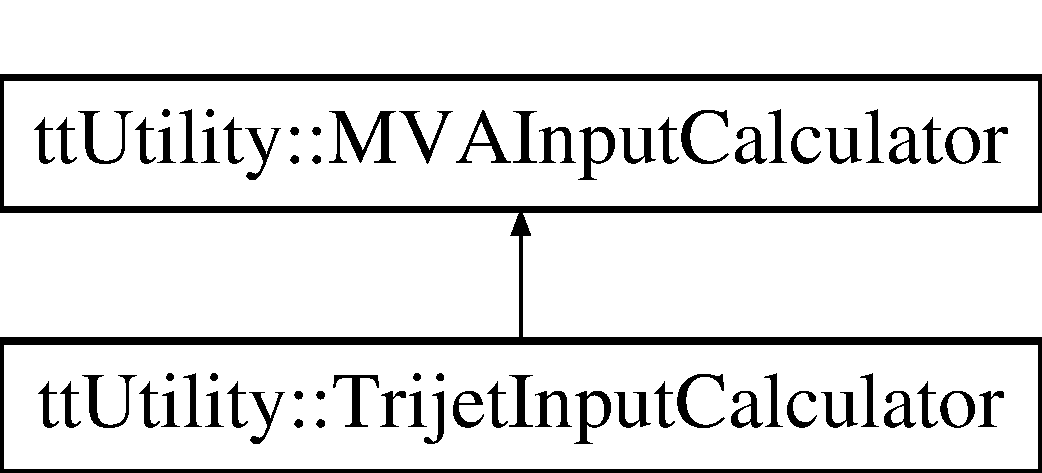
\includegraphics[height=2.000000cm]{classttUtility_1_1TrijetInputCalculator}
\end{center}
\end{figure}
\subsection*{Public Member Functions}
\begin{DoxyCompactItemize}
\item 
void \hyperlink{classttUtility_1_1TrijetInputCalculator_ae51335839fc75caf28e4ec030a3cfb40}{map\-Vars} (const std\-::vector$<$ std\-::string $>$ \&, float $\ast$)
\item 
bool \hyperlink{classttUtility_1_1TrijetInputCalculator_a02c32e65787b891edfe9b85c32aff8b0}{calculate\-Vars} (const \hyperlink{classTopObject}{Top\-Object} \&)
\end{DoxyCompactItemize}


\subsection{Detailed Description}
Class to calculate the input variables for the A\-K4 based resolved top catagory 

\subsection{Member Function Documentation}
\hypertarget{classttUtility_1_1TrijetInputCalculator_a02c32e65787b891edfe9b85c32aff8b0}{\index{tt\-Utility\-::\-Trijet\-Input\-Calculator@{tt\-Utility\-::\-Trijet\-Input\-Calculator}!calculate\-Vars@{calculate\-Vars}}
\index{calculate\-Vars@{calculate\-Vars}!ttUtility::TrijetInputCalculator@{tt\-Utility\-::\-Trijet\-Input\-Calculator}}
\subsubsection[{calculate\-Vars}]{\setlength{\rightskip}{0pt plus 5cm}bool tt\-Utility\-::\-Trijet\-Input\-Calculator\-::calculate\-Vars (
\begin{DoxyParamCaption}
\item[{const {\bf Top\-Object} \&}]{}
\end{DoxyParamCaption}
)\hspace{0.3cm}{\ttfamily [virtual]}}}\label{classttUtility_1_1TrijetInputCalculator_a02c32e65787b891edfe9b85c32aff8b0}
Calculate the requested variables and store the values directly in the input array for the M\-V\-A 
\begin{DoxyParams}{Parameters}
{\em top\-Cand} & the top candidate to calculate the input variables for \\
\hline
\end{DoxyParams}


Implements \hyperlink{classttUtility_1_1MVAInputCalculator_ac48dbe37b01a207150537c86e9f85038}{tt\-Utility\-::\-M\-V\-A\-Input\-Calculator}.

\hypertarget{classttUtility_1_1TrijetInputCalculator_ae51335839fc75caf28e4ec030a3cfb40}{\index{tt\-Utility\-::\-Trijet\-Input\-Calculator@{tt\-Utility\-::\-Trijet\-Input\-Calculator}!map\-Vars@{map\-Vars}}
\index{map\-Vars@{map\-Vars}!ttUtility::TrijetInputCalculator@{tt\-Utility\-::\-Trijet\-Input\-Calculator}}
\subsubsection[{map\-Vars}]{\setlength{\rightskip}{0pt plus 5cm}void tt\-Utility\-::\-Trijet\-Input\-Calculator\-::map\-Vars (
\begin{DoxyParamCaption}
\item[{const std\-::vector$<$ std\-::string $>$ \&}]{, }
\item[{float $\ast$}]{}
\end{DoxyParamCaption}
)\hspace{0.3cm}{\ttfamily [virtual]}}}\label{classttUtility_1_1TrijetInputCalculator_ae51335839fc75caf28e4ec030a3cfb40}
The job of map\-Vars is to populate the internal pointers for all variables in the input variable list with their memory location in the data array. To be called only once for the creation of the array pointed to by data. 
\begin{DoxyParams}{Parameters}
{\em vars} & list of variables used for the model \\
\hline
{\em data} & pointer to start of the data array which willbe used as input to the M\-V\-A \\
\hline
\end{DoxyParams}


Implements \hyperlink{classttUtility_1_1MVAInputCalculator_a9fd6fa53268079fa590b86ee9791c344}{tt\-Utility\-::\-M\-V\-A\-Input\-Calculator}.



The documentation for this class was generated from the following files\-:\begin{DoxyCompactItemize}
\item 
/home/travis/build/susy2015/\-Top\-Tagger/\-Top\-Tagger/include/\hyperlink{TopTaggerUtilities_8h}{Top\-Tagger\-Utilities.\-h}\item 
/home/travis/build/susy2015/\-Top\-Tagger/\-Top\-Tagger/src/Top\-Tagger\-Utilities.\-cpp\end{DoxyCompactItemize}

\hypertarget{classTTException}{\section{T\-T\-Exception Class Reference}
\label{classTTException}\index{T\-T\-Exception@{T\-T\-Exception}}
}
\subsection*{Public Member Functions}
\begin{DoxyCompactItemize}
\item 
\hypertarget{classTTException_a9b4ef38abc1a5944eea011d63f7574e1}{{\bfseries T\-T\-Exception} (const int, const std\-::string, const std\-::string, const std\-::string)}\label{classTTException_a9b4ef38abc1a5944eea011d63f7574e1}

\item 
\hypertarget{classTTException_a0438e0a4023264e996288ac23581e0c3}{int {\bfseries get\-Line\-Number} () const }\label{classTTException_a0438e0a4023264e996288ac23581e0c3}

\item 
\hypertarget{classTTException_a342c0204e296e2fdae3b60b12d348592}{std\-::string {\bfseries get\-Function\-Name} () const }\label{classTTException_a342c0204e296e2fdae3b60b12d348592}

\item 
\hypertarget{classTTException_a3d7570a3fd6f0702069be6450e3c6a63}{std\-::string {\bfseries get\-File\-Name} () const }\label{classTTException_a3d7570a3fd6f0702069be6450e3c6a63}

\item 
\hypertarget{classTTException_ac37882c84da17e0e2c78637e97ba4b09}{std\-::string {\bfseries get\-Message} () const }\label{classTTException_ac37882c84da17e0e2c78637e97ba4b09}

\item 
\hypertarget{classTTException_a13d5fa6996d8add8df255df6415bc46a}{std\-::string {\bfseries get\-Print\-Message} () const }\label{classTTException_a13d5fa6996d8add8df255df6415bc46a}

\item 
\hypertarget{classTTException_ab67669a727365d75c4dbd63860bf7c85}{void {\bfseries print} () const }\label{classTTException_ab67669a727365d75c4dbd63860bf7c85}

\end{DoxyCompactItemize}


The documentation for this class was generated from the following files\-:\begin{DoxyCompactItemize}
\item 
/home/travis/build/susy2015/\-Top\-Tagger/\-Cfg\-Parser/include/T\-T\-Exception.\-h\item 
/home/travis/build/susy2015/\-Top\-Tagger/\-Cfg\-Parser/src/T\-T\-Exception.\-cpp\end{DoxyCompactItemize}

\hypertarget{classTTMAK8TopFilter}{\section{T\-T\-M\-A\-K8\-Top\-Filter Class Reference}
\label{classTTMAK8TopFilter}\index{T\-T\-M\-A\-K8\-Top\-Filter@{T\-T\-M\-A\-K8\-Top\-Filter}}
}
Inheritance diagram for T\-T\-M\-A\-K8\-Top\-Filter\-:\begin{figure}[H]
\begin{center}
\leavevmode
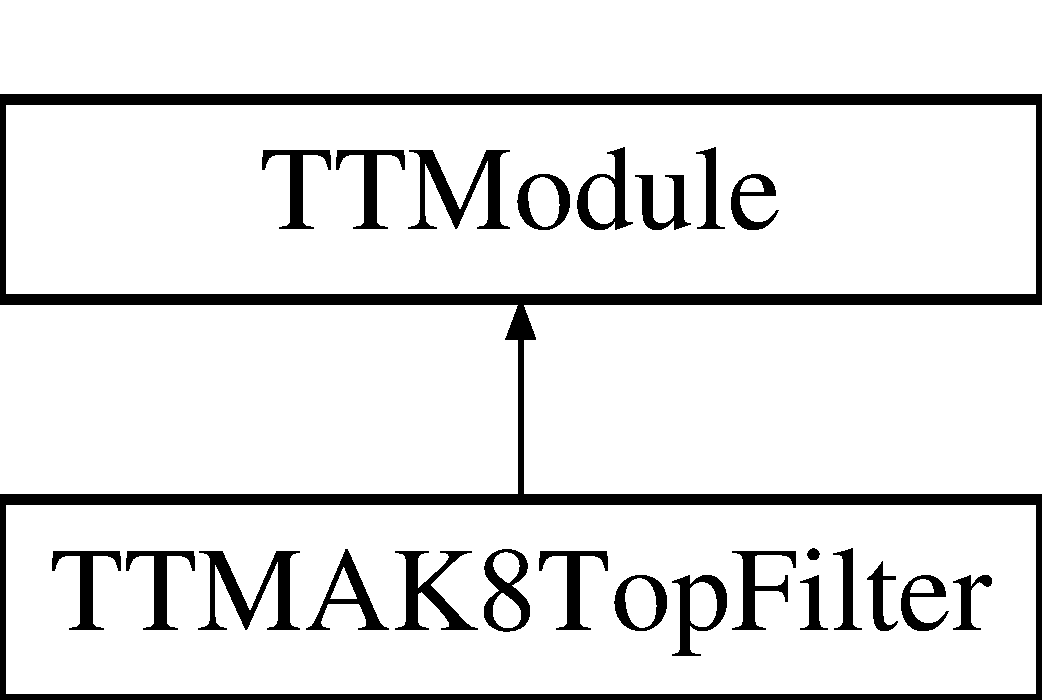
\includegraphics[height=2.000000cm]{classTTMAK8TopFilter}
\end{center}
\end{figure}
\subsection*{Public Member Functions}
\begin{DoxyCompactItemize}
\item 
void \hyperlink{classTTMAK8TopFilter_aed52bd6877ec9b8ac3a2f45769f05856}{get\-Parameters} (const \hyperlink{classcfg_1_1CfgDocument}{cfg\-::\-Cfg\-Document} $\ast$, const std\-::string \&)
\item 
void \hyperlink{classTTMAK8TopFilter_a28a8fcd8a829caae32b2a106037d3a6f}{run} (\hyperlink{classTopTaggerResults}{Top\-Tagger\-Results} \&)
\end{DoxyCompactItemize}


\subsection{Member Function Documentation}
\hypertarget{classTTMAK8TopFilter_aed52bd6877ec9b8ac3a2f45769f05856}{\index{T\-T\-M\-A\-K8\-Top\-Filter@{T\-T\-M\-A\-K8\-Top\-Filter}!get\-Parameters@{get\-Parameters}}
\index{get\-Parameters@{get\-Parameters}!TTMAK8TopFilter@{T\-T\-M\-A\-K8\-Top\-Filter}}
\subsubsection[{get\-Parameters}]{\setlength{\rightskip}{0pt plus 5cm}void T\-T\-M\-A\-K8\-Top\-Filter\-::get\-Parameters (
\begin{DoxyParamCaption}
\item[{const {\bf cfg\-::\-Cfg\-Document} $\ast$}]{, }
\item[{const std\-::string \&}]{}
\end{DoxyParamCaption}
)\hspace{0.3cm}{\ttfamily [virtual]}}}\label{classTTMAK8TopFilter_aed52bd6877ec9b8ac3a2f45769f05856}
This function is called by \hyperlink{classTopTagger}{Top\-Tagger} to configure each module based upon the information present in the configuration file. The inputs for this function are provided by \hyperlink{classTopTagger}{Top\-Tagger} and are the configuration document object and the local context string for this module. The local context string defines where to look in the configuration file for the local parameters. 

Implements \hyperlink{classTTModule_aa9d2842c9e94782059fe92044a68e3a6}{T\-T\-Module}.

\hypertarget{classTTMAK8TopFilter_a28a8fcd8a829caae32b2a106037d3a6f}{\index{T\-T\-M\-A\-K8\-Top\-Filter@{T\-T\-M\-A\-K8\-Top\-Filter}!run@{run}}
\index{run@{run}!TTMAK8TopFilter@{T\-T\-M\-A\-K8\-Top\-Filter}}
\subsubsection[{run}]{\setlength{\rightskip}{0pt plus 5cm}void T\-T\-M\-A\-K8\-Top\-Filter\-::run (
\begin{DoxyParamCaption}
\item[{{\bf Top\-Tagger\-Results} \&}]{}
\end{DoxyParamCaption}
)\hspace{0.3cm}{\ttfamily [virtual]}}}\label{classTTMAK8TopFilter_a28a8fcd8a829caae32b2a106037d3a6f}
run is called automatically by \hyperlink{classTopTagger}{Top\-Tagger} once per event to run th emodule. The module interfaces with other modules through the \hyperlink{classTopTaggerResults}{Top\-Tagger\-Results} object which is passed as a non-\/const reference from \hyperlink{classTopTagger}{Top\-Tagger}. 

Implements \hyperlink{classTTModule_a14e7c03fbf4ee1a5008c9344adc7c896}{T\-T\-Module}.



The documentation for this class was generated from the following files\-:\begin{DoxyCompactItemize}
\item 
/home/travis/build/susy2015/\-Top\-Tagger/\-Top\-Tagger/include/T\-T\-M\-A\-K8\-Top\-Filter.\-h\item 
/home/travis/build/susy2015/\-Top\-Tagger/\-Top\-Tagger/src/T\-T\-M\-A\-K8\-Top\-Filter.\-cpp\end{DoxyCompactItemize}

\hypertarget{classTTMBasicClusterAlgo}{\section{T\-T\-M\-Basic\-Cluster\-Algo Class Reference}
\label{classTTMBasicClusterAlgo}\index{T\-T\-M\-Basic\-Cluster\-Algo@{T\-T\-M\-Basic\-Cluster\-Algo}}
}


{\ttfamily \#include $<$T\-T\-M\-Basic\-Cluster\-Algo.\-h$>$}

Inheritance diagram for T\-T\-M\-Basic\-Cluster\-Algo\-:\begin{figure}[H]
\begin{center}
\leavevmode
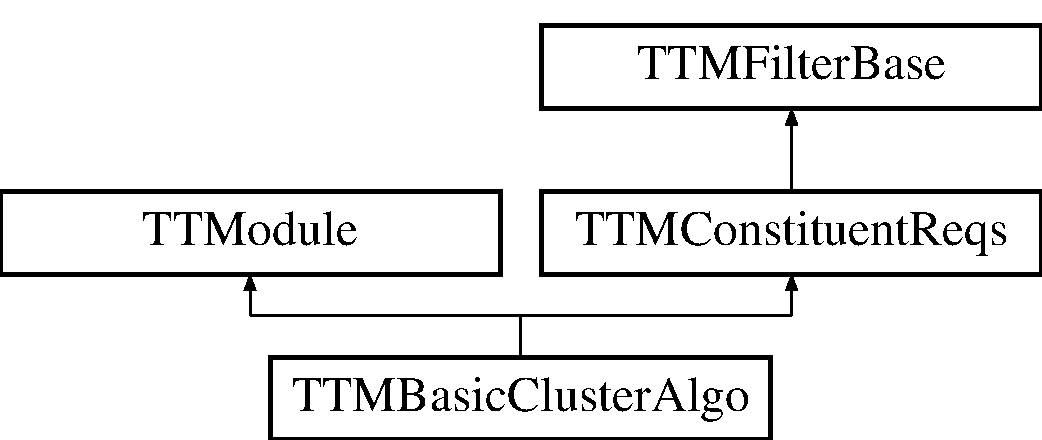
\includegraphics[height=3.000000cm]{classTTMBasicClusterAlgo}
\end{center}
\end{figure}
\subsection*{Public Member Functions}
\begin{DoxyCompactItemize}
\item 
void \hyperlink{classTTMBasicClusterAlgo_afdbe472d26a753268dac63d897169299}{get\-Parameters} (const \hyperlink{classcfg_1_1CfgDocument}{cfg\-::\-Cfg\-Document} $\ast$, const std\-::string \&)
\item 
void \hyperlink{classTTMBasicClusterAlgo_ae1d464bf1db5762318766d109c843932}{run} (\hyperlink{classTopTaggerResults}{Top\-Tagger\-Results} \&)
\end{DoxyCompactItemize}
\subsection*{Additional Inherited Members}


\subsection{Detailed Description}
This module is used to cluster top candidates using a combination of A\-K4 and A\-K8 jets. This algorithm uses A\-K8 jets for the merged W and top candidates, and A\-K4 jets for the resolved category as well as to combine with W jets to for top candidates. This module is capable of clustering trijet (resolved tops), dijet (W+jet), and monojet (fully merged top) candidates.


\begin{DoxyParams}{Parameters}
{\em do\-Trijet} & (bool) Enable the resolved top category clustering. \\
\hline
{\em min\-Top\-Cand\-Mass} & (float) Minimum trijet mass for resolved candidates \\
\hline
{\em max\-Top\-Cand\-Mass} & (float) Maximum trijet mass for resolved candidates \\
\hline
{\em d\-R\-Max\-Trijet} & (float) The maximum d\-R seperation between any A\-K4 jet and te trijet centroid for resolved A\-K4 candidates to be considered as a top candidate. \\
\hline
{\em nb\-Seed} & (int) If greater than 0, the number of highest b-\/tag discriminator jets to use as clustering seeds for trijet candidates. (Default -\/1) \\
\hline
{\em min\-Trijet\-A\-K4\-Jet\-Pt} & (float) Minimum pt threshold for the lowest pt A\-K4 jet in th etrijet candidate. \\
\hline
{\em mid\-Trijet\-A\-K4\-Jet\-Pt} & (float) Minimum pt threshold for the medium pt A\-K4 jet in th etrijet candidate. \\
\hline
{\em max\-Trijet\-A\-K4\-Jet\-Pt} & (float) Minimum pt threshold for the highest pt A\-K4 jet in th etrijet candidate. \\
\hline
{\em do\-Dijet} & (bool) Enable the A\-K8\-W + A\-K4 jet category clustering. \\
\hline
{\em d\-R\-Max\-Dijet} & (float) The maximum allowed seperation if d\-R between the A\-K4 and A\-K8 jet and the dijet centroid for the dijet catagory. \\
\hline
{\em do\-Monojet} & (bool) Enable the fully merged top category clustering. \\
\hline
{\em use\-Deep\-A\-K8} & (bool) Use deep\-A\-K8 discriminator to identify boosted objects from A\-K8 jets instead of N\-Subjettiness.\\
\hline
\end{DoxyParams}
See \hyperlink{classTTMConstituentReqs}{T\-T\-M\-Constituent\-Reqs} for more parameters 

\subsection{Member Function Documentation}
\hypertarget{classTTMBasicClusterAlgo_afdbe472d26a753268dac63d897169299}{\index{T\-T\-M\-Basic\-Cluster\-Algo@{T\-T\-M\-Basic\-Cluster\-Algo}!get\-Parameters@{get\-Parameters}}
\index{get\-Parameters@{get\-Parameters}!TTMBasicClusterAlgo@{T\-T\-M\-Basic\-Cluster\-Algo}}
\subsubsection[{get\-Parameters}]{\setlength{\rightskip}{0pt plus 5cm}void T\-T\-M\-Basic\-Cluster\-Algo\-::get\-Parameters (
\begin{DoxyParamCaption}
\item[{const {\bf cfg\-::\-Cfg\-Document} $\ast$}]{, }
\item[{const std\-::string \&}]{}
\end{DoxyParamCaption}
)\hspace{0.3cm}{\ttfamily [virtual]}}}\label{classTTMBasicClusterAlgo_afdbe472d26a753268dac63d897169299}
This function is called by \hyperlink{classTopTagger}{Top\-Tagger} to configure each module based upon the information present in the configuration file. The inputs for this function are provided by \hyperlink{classTopTagger}{Top\-Tagger} and are the configuration document object and the local context string for this module. The local context string defines where to look in the configuration file for the local parameters. 

Implements \hyperlink{classTTModule_aa9d2842c9e94782059fe92044a68e3a6}{T\-T\-Module}.

\hypertarget{classTTMBasicClusterAlgo_ae1d464bf1db5762318766d109c843932}{\index{T\-T\-M\-Basic\-Cluster\-Algo@{T\-T\-M\-Basic\-Cluster\-Algo}!run@{run}}
\index{run@{run}!TTMBasicClusterAlgo@{T\-T\-M\-Basic\-Cluster\-Algo}}
\subsubsection[{run}]{\setlength{\rightskip}{0pt plus 5cm}void T\-T\-M\-Basic\-Cluster\-Algo\-::run (
\begin{DoxyParamCaption}
\item[{{\bf Top\-Tagger\-Results} \&}]{}
\end{DoxyParamCaption}
)\hspace{0.3cm}{\ttfamily [virtual]}}}\label{classTTMBasicClusterAlgo_ae1d464bf1db5762318766d109c843932}
run is called automatically by \hyperlink{classTopTagger}{Top\-Tagger} once per event to run th emodule. The module interfaces with other modules through the \hyperlink{classTopTaggerResults}{Top\-Tagger\-Results} object which is passed as a non-\/const reference from \hyperlink{classTopTagger}{Top\-Tagger}. 

Implements \hyperlink{classTTModule_a14e7c03fbf4ee1a5008c9344adc7c896}{T\-T\-Module}.



The documentation for this class was generated from the following files\-:\begin{DoxyCompactItemize}
\item 
/home/travis/build/susy2015/\-Top\-Tagger/\-Top\-Tagger/include/T\-T\-M\-Basic\-Cluster\-Algo.\-h\item 
/home/travis/build/susy2015/\-Top\-Tagger/\-Top\-Tagger/src/T\-T\-M\-Basic\-Cluster\-Algo.\-cpp\end{DoxyCompactItemize}

\hypertarget{classTTMConstituentReqs}{\section{T\-T\-M\-Constituent\-Reqs Class Reference}
\label{classTTMConstituentReqs}\index{T\-T\-M\-Constituent\-Reqs@{T\-T\-M\-Constituent\-Reqs}}
}


{\ttfamily \#include $<$T\-T\-M\-Constituent\-Reqs.\-h$>$}

Inheritance diagram for T\-T\-M\-Constituent\-Reqs\-:\begin{figure}[H]
\begin{center}
\leavevmode
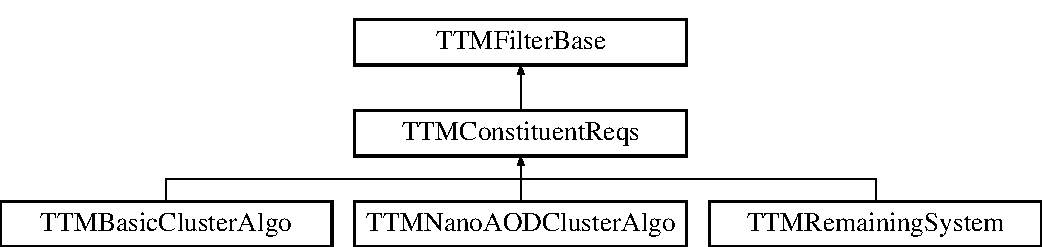
\includegraphics[height=3.000000cm]{classTTMConstituentReqs}
\end{center}
\end{figure}
\subsection*{Protected Member Functions}
\begin{DoxyCompactItemize}
\item 
\hypertarget{classTTMConstituentReqs_a24ed62136b9c36fa4a987a12e43d8abe}{bool \hyperlink{classTTMConstituentReqs_a24ed62136b9c36fa4a987a12e43d8abe}{pass\-A\-K8\-W\-Reqs} (const \hyperlink{classConstituent}{Constituent} \&constituent) const }\label{classTTMConstituentReqs_a24ed62136b9c36fa4a987a12e43d8abe}

\begin{DoxyCompactList}\small\item\em Implement the requirements to be tagged as an A\-K8 W. \end{DoxyCompactList}\item 
\hypertarget{classTTMConstituentReqs_ad2ff0cdbd2576c566ccf86be56c17626}{bool \hyperlink{classTTMConstituentReqs_ad2ff0cdbd2576c566ccf86be56c17626}{pass\-A\-K4\-W\-Reqs} (const \hyperlink{classConstituent}{Constituent} \&constituent, const \hyperlink{classConstituent}{Constituent} \&constituent\-A\-K8) const }\label{classTTMConstituentReqs_ad2ff0cdbd2576c566ccf86be56c17626}

\begin{DoxyCompactList}\small\item\em Implement the requirements for A\-K4 jets to partner with A\-K8 W. \end{DoxyCompactList}\item 
\hypertarget{classTTMConstituentReqs_af02e6acd3232253af0baf72a6c69a8a5}{bool \hyperlink{classTTMConstituentReqs_af02e6acd3232253af0baf72a6c69a8a5}{pass\-A\-K8\-Top\-Reqs} (const \hyperlink{classConstituent}{Constituent} \&constituent) const }\label{classTTMConstituentReqs_af02e6acd3232253af0baf72a6c69a8a5}

\begin{DoxyCompactList}\small\item\em Implement the requirements to be tagged as an A\-K8 top. \end{DoxyCompactList}\item 
\hypertarget{classTTMConstituentReqs_a146535ca0b3c55a3178dff46d8312371}{bool \hyperlink{classTTMConstituentReqs_a146535ca0b3c55a3178dff46d8312371}{pass\-A\-K4\-Resolved\-Reqs} (const \hyperlink{classConstituent}{Constituent} \&constituent, const double min\-Pt) const }\label{classTTMConstituentReqs_a146535ca0b3c55a3178dff46d8312371}

\begin{DoxyCompactList}\small\item\em Implement the requirements for the A\-K4 resolved constituents. \end{DoxyCompactList}\item 
\hypertarget{classTTMConstituentReqs_ad315aa8b3bbcaa2194e515876f6ae85f}{bool \hyperlink{classTTMConstituentReqs_ad315aa8b3bbcaa2194e515876f6ae85f}{pass\-Deep\-A\-K8\-W\-Reqs} (const \hyperlink{classConstituent}{Constituent} \&constituent) const }\label{classTTMConstituentReqs_ad315aa8b3bbcaa2194e515876f6ae85f}

\begin{DoxyCompactList}\small\item\em Implement requirements on A\-K8 W tagged with deep\-A\-K8. \end{DoxyCompactList}\item 
\hypertarget{classTTMConstituentReqs_a3fa336ca887104b5ec315db546bb5b36}{bool \hyperlink{classTTMConstituentReqs_a3fa336ca887104b5ec315db546bb5b36}{pass\-Deep\-A\-K8\-Top\-Reqs} (const \hyperlink{classConstituent}{Constituent} \&constituent) const }\label{classTTMConstituentReqs_a3fa336ca887104b5ec315db546bb5b36}

\begin{DoxyCompactList}\small\item\em Implement requirements on A\-K8 tops tagged with deep\-A\-K8. \end{DoxyCompactList}\item 
\hypertarget{classTTMConstituentReqs_a6b72bd3d3605f24c240053a9ac0f36df}{void \hyperlink{classTTMConstituentReqs_a6b72bd3d3605f24c240053a9ac0f36df}{get\-Parameters} (const \hyperlink{classcfg_1_1CfgDocument}{cfg\-::\-Cfg\-Document} $\ast$, const std\-::string \&)}\label{classTTMConstituentReqs_a6b72bd3d3605f24c240053a9ac0f36df}

\begin{DoxyCompactList}\small\item\em Get the parameters needed for the constituent selection functions. \end{DoxyCompactList}\end{DoxyCompactItemize}
\subsection*{Protected Attributes}
\begin{DoxyCompactItemize}
\item 
\hypertarget{classTTMConstituentReqs_ac98f4b266d20f9975e338620d5c72425}{double {\bfseries d\-R\-Match\-\_\-}}\label{classTTMConstituentReqs_ac98f4b266d20f9975e338620d5c72425}

\item 
\hypertarget{classTTMConstituentReqs_ae1b896324fc5546fa998f7b343da4a73}{double {\bfseries d\-R\-Match\-A\-K8\-\_\-}}\label{classTTMConstituentReqs_ae1b896324fc5546fa998f7b343da4a73}

\item 
\hypertarget{classTTMConstituentReqs_a6a778c0d25d85ccc4d87a7a630d38e53}{double {\bfseries min\-A\-K8\-Top\-Mass\-\_\-}}\label{classTTMConstituentReqs_a6a778c0d25d85ccc4d87a7a630d38e53}

\item 
\hypertarget{classTTMConstituentReqs_aceba29666244cb7ee7fc76780c2a0abb}{double {\bfseries max\-A\-K8\-Top\-Mass\-\_\-}}\label{classTTMConstituentReqs_aceba29666244cb7ee7fc76780c2a0abb}

\item 
\hypertarget{classTTMConstituentReqs_a5ae6e7ff4901fa0906c5e44538deb986}{double {\bfseries max\-Top\-Tau32\-\_\-}}\label{classTTMConstituentReqs_a5ae6e7ff4901fa0906c5e44538deb986}

\item 
\hypertarget{classTTMConstituentReqs_a1278553c3950ec8057c4860997024a69}{double {\bfseries min\-A\-K8\-Top\-Pt\-\_\-}}\label{classTTMConstituentReqs_a1278553c3950ec8057c4860997024a69}

\item 
\hypertarget{classTTMConstituentReqs_aca47798ffce469f8a43b825798693c72}{double {\bfseries deep\-A\-K8\-W\-Disc\-\_\-}}\label{classTTMConstituentReqs_aca47798ffce469f8a43b825798693c72}

\item 
\hypertarget{classTTMConstituentReqs_ac182ac9699ded5d0aefff19ecefe7570}{double {\bfseries deep\-A\-K8\-Top\-Disc\-\_\-}}\label{classTTMConstituentReqs_ac182ac9699ded5d0aefff19ecefe7570}

\item 
\hypertarget{classTTMConstituentReqs_aef537173e73a40069b42d0ef5e14daa8}{double {\bfseries min\-A\-K8\-W\-Mass\-\_\-}}\label{classTTMConstituentReqs_aef537173e73a40069b42d0ef5e14daa8}

\item 
\hypertarget{classTTMConstituentReqs_a79fe4f3ece12c5dc280793becb71b8b2}{double {\bfseries max\-A\-K8\-W\-Mass\-\_\-}}\label{classTTMConstituentReqs_a79fe4f3ece12c5dc280793becb71b8b2}

\item 
\hypertarget{classTTMConstituentReqs_ac4475ca59a99f5a3b54390413e7aa87e}{double {\bfseries max\-W\-Tau21\-\_\-}}\label{classTTMConstituentReqs_ac4475ca59a99f5a3b54390413e7aa87e}

\item 
\hypertarget{classTTMConstituentReqs_aad794bd881baebbbbb83f7042e291999}{double {\bfseries min\-A\-K8\-W\-Pt\-\_\-}}\label{classTTMConstituentReqs_aad794bd881baebbbbb83f7042e291999}

\item 
\hypertarget{classTTMConstituentReqs_a40ece9d7d687f58842ebe8ad70bb47fa}{double {\bfseries min\-A\-K4\-W\-Pt\-\_\-}}\label{classTTMConstituentReqs_a40ece9d7d687f58842ebe8ad70bb47fa}

\end{DoxyCompactItemize}


\subsection{Detailed Description}
This class implemens common selection requirements for constituents for use in other modules, but is not itself a T\-T Module


\begin{DoxyParams}{Parameters}
{\em d\-R\-Match} & (float) {\bfseries  common context } The d\-R requirement used to select whether an A\-K4 jet matches a A\-K8 subjet \\
\hline
{\em min\-A\-K8\-Top\-Mass} & (float) Minimum A\-K8 mass to be considered an A\-K8 top candidate. \\
\hline
{\em max\-A\-K8\-Top\-Mass} & (float) Maximum A\-K8 mass to be considered an A\-K8 top candidate. \\
\hline
{\em max\-Top\-Tau32} & (float) Maximum of the Nsubjettiness ratio tau3/tau2 to be considered an A\-K8 top candidate. \\
\hline
{\em deep\-A\-K8\-Top\-Disc} & (float) Minimum deep\-A\-K8 discriminator threshold to be considered an A\-K8 top candidate. \\
\hline
{\em min\-A\-K8\-Top\-Pt} & (float) Minimum top pt to be considered as an A\-K8 top candidate. \\
\hline
{\em min\-A\-K8\-W\-Mass} & (float) Minimum A\-K8 mass to be considered an A\-K8 W candidate. \\
\hline
{\em max\-A\-K8\-W\-Mass} & (float) Maximum A\-K8 mass to be considered an A\-K8 W candidate. \\
\hline
{\em max\-W\-Tau21} & (float) Maximum of the Nsubjettiness ratio tau2/tau1 to be considered an A\-K8 W candidate. \\
\hline
{\em deep\-A\-K8\-W\-Disc} & (float) Minimum deep\-A\-K8 discriminator threshold to be considered an A\-K8 W candidate. \\
\hline
{\em min\-A\-K8\-W\-Pt} & (float) Minimum top A\-K8 jet pt to be considered as an A\-K8 + A\-K4 top candidate. \\
\hline
{\em min\-A\-K4\-W\-Pt} & (float) Minimum top A\-K4 jet pt to be considered as an A\-K8 + A\-K4 top candidate. \\
\hline
\end{DoxyParams}


The documentation for this class was generated from the following files\-:\begin{DoxyCompactItemize}
\item 
/home/travis/build/susy2015/\-Top\-Tagger/\-Top\-Tagger/include/T\-T\-M\-Constituent\-Reqs.\-h\item 
/home/travis/build/susy2015/\-Top\-Tagger/\-Top\-Tagger/src/T\-T\-M\-Constituent\-Reqs.\-cpp\end{DoxyCompactItemize}

\hypertarget{classTTMDiscriminatorFilter}{\section{T\-T\-M\-Discriminator\-Filter Class Reference}
\label{classTTMDiscriminatorFilter}\index{T\-T\-M\-Discriminator\-Filter@{T\-T\-M\-Discriminator\-Filter}}
}


{\ttfamily \#include $<$T\-T\-M\-Discriminator\-Filter.\-h$>$}

Inheritance diagram for T\-T\-M\-Discriminator\-Filter\-:\begin{figure}[H]
\begin{center}
\leavevmode
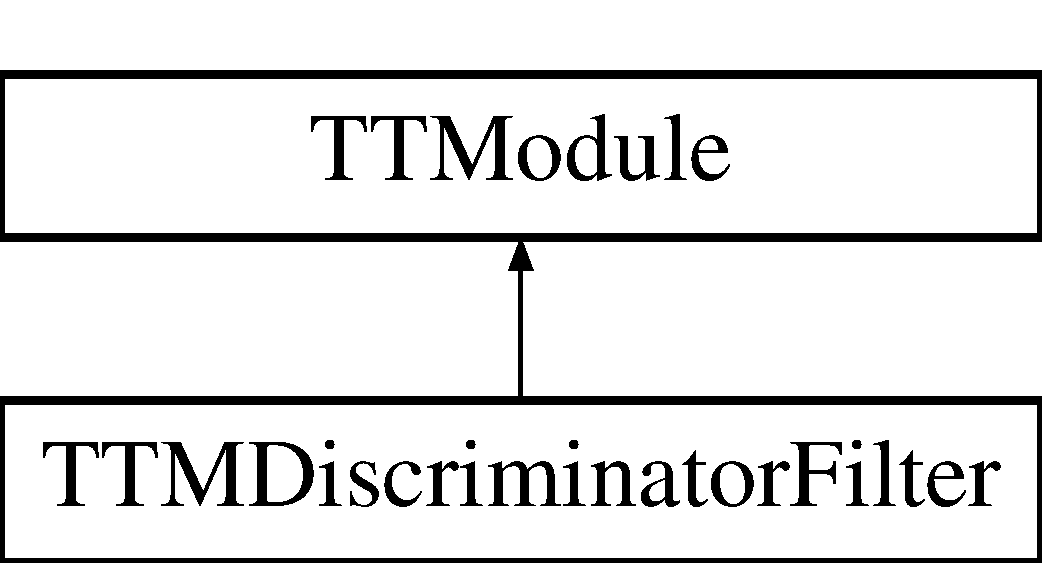
\includegraphics[height=2.000000cm]{classTTMDiscriminatorFilter}
\end{center}
\end{figure}
\subsection*{Public Member Functions}
\begin{DoxyCompactItemize}
\item 
void \hyperlink{classTTMDiscriminatorFilter_afffc488bca7ff5cc89fc436edc927f9e}{get\-Parameters} (const \hyperlink{classcfg_1_1CfgDocument}{cfg\-::\-Cfg\-Document} $\ast$, const std\-::string \&)
\item 
void \hyperlink{classTTMDiscriminatorFilter_a72dbc7e987d75bcf96837f313d31d999}{run} (\hyperlink{classTopTaggerResults}{Top\-Tagger\-Results} \&)
\end{DoxyCompactItemize}
\subsection*{Additional Inherited Members}


\subsection{Detailed Description}
This module implements an interface to Tensorflow through the tensorflow c-\/api for filtering top candidates. This module places top candidates which pass the requirements directly into the final top list.


\begin{DoxyParams}{Parameters}
{\em disc\-Cut} & (float) Highest minimum discriminator threshold allowed (If disc\-Offest is set $>$ 1 and disc\-Slope is positive then this serves as a basic discriminator threshold) \\
\hline
{\em disc\-Offset} & (float) Discriminator cut for zero pt top candidates \\
\hline
{\em disc\-Slope} & (float) Pt dependent slopt for discriminator cut \\
\hline
{\em type} & (int) Type of constituent to apply selection to (1 -\/ monojet, 2 -\/ dijet, 3 -\/ trijet) \\
\hline
{\em bdisc\-Threshold} & (float) Threshold on b-\/tag discriminator to be considered a b-\/jet. \\
\hline
{\em b\-Eta\-Cut} & (float) Requirment on $\vert$eta$\vert$ for a constituent to be considered a b-\/jet \\
\hline
{\em max\-Nb\-In\-Top} & (int) The maximum number of constituent jets which can be b-\/tagged for the candidate to be a final top (set $<$ 0 to disable) \\
\hline
\end{DoxyParams}


\subsection{Member Function Documentation}
\hypertarget{classTTMDiscriminatorFilter_afffc488bca7ff5cc89fc436edc927f9e}{\index{T\-T\-M\-Discriminator\-Filter@{T\-T\-M\-Discriminator\-Filter}!get\-Parameters@{get\-Parameters}}
\index{get\-Parameters@{get\-Parameters}!TTMDiscriminatorFilter@{T\-T\-M\-Discriminator\-Filter}}
\subsubsection[{get\-Parameters}]{\setlength{\rightskip}{0pt plus 5cm}void T\-T\-M\-Discriminator\-Filter\-::get\-Parameters (
\begin{DoxyParamCaption}
\item[{const {\bf cfg\-::\-Cfg\-Document} $\ast$}]{, }
\item[{const std\-::string \&}]{}
\end{DoxyParamCaption}
)\hspace{0.3cm}{\ttfamily [virtual]}}}\label{classTTMDiscriminatorFilter_afffc488bca7ff5cc89fc436edc927f9e}
This function is called by \hyperlink{classTopTagger}{Top\-Tagger} to configure each module based upon the information present in the configuration file. The inputs for this function are provided by \hyperlink{classTopTagger}{Top\-Tagger} and are the configuration document object and the local context string for this module. The local context string defines where to look in the configuration file for the local parameters. 

Implements \hyperlink{classTTModule_aa9d2842c9e94782059fe92044a68e3a6}{T\-T\-Module}.

\hypertarget{classTTMDiscriminatorFilter_a72dbc7e987d75bcf96837f313d31d999}{\index{T\-T\-M\-Discriminator\-Filter@{T\-T\-M\-Discriminator\-Filter}!run@{run}}
\index{run@{run}!TTMDiscriminatorFilter@{T\-T\-M\-Discriminator\-Filter}}
\subsubsection[{run}]{\setlength{\rightskip}{0pt plus 5cm}void T\-T\-M\-Discriminator\-Filter\-::run (
\begin{DoxyParamCaption}
\item[{{\bf Top\-Tagger\-Results} \&}]{}
\end{DoxyParamCaption}
)\hspace{0.3cm}{\ttfamily [virtual]}}}\label{classTTMDiscriminatorFilter_a72dbc7e987d75bcf96837f313d31d999}
run is called automatically by \hyperlink{classTopTagger}{Top\-Tagger} once per event to run th emodule. The module interfaces with other modules through the \hyperlink{classTopTaggerResults}{Top\-Tagger\-Results} object which is passed as a non-\/const reference from \hyperlink{classTopTagger}{Top\-Tagger}. 

Implements \hyperlink{classTTModule_a14e7c03fbf4ee1a5008c9344adc7c896}{T\-T\-Module}.



The documentation for this class was generated from the following files\-:\begin{DoxyCompactItemize}
\item 
/home/travis/build/susy2015/\-Top\-Tagger/\-Top\-Tagger/interface/T\-T\-M\-Discriminator\-Filter.\-h\item 
/home/travis/build/susy2015/\-Top\-Tagger/\-Top\-Tagger/src/T\-T\-M\-Discriminator\-Filter.\-cpp\end{DoxyCompactItemize}

\hypertarget{classTTMFactory}{\section{T\-T\-M\-Factory Class Reference}
\label{classTTMFactory}\index{T\-T\-M\-Factory@{T\-T\-M\-Factory}}
}


{\ttfamily \#include $<$T\-T\-M\-Factory.\-h$>$}

\subsection*{Static Public Member Functions}
\begin{DoxyCompactItemize}
\item 
\hypertarget{classTTMFactory_a728fa564c6c1e78450c69a9a875746da}{static \hyperlink{classTTMFactory}{T\-T\-M\-Factory} $\ast$ \hyperlink{classTTMFactory_a728fa564c6c1e78450c69a9a875746da}{get\-Instance} ()}\label{classTTMFactory_a728fa564c6c1e78450c69a9a875746da}

\begin{DoxyCompactList}\small\item\em Get the static instance of the factory (or make it if it does not exist) \end{DoxyCompactList}\item 
\hypertarget{classTTMFactory_a4651a7e0c90b7c36acbdada8de05a4b4}{static bool \hyperlink{classTTMFactory_a4651a7e0c90b7c36acbdada8de05a4b4}{register\-Module} (const std\-::string \&, std\-::function$<$ \hyperlink{classTTModule}{T\-T\-Module} $\ast$()$>$)}\label{classTTMFactory_a4651a7e0c90b7c36acbdada8de05a4b4}

\begin{DoxyCompactList}\small\item\em register a new module in the map, this is called automatically by the magic macro \char`\"{}\-R\-E\-G\-I\-S\-T\-E\-R\-\_\-\-T\-T\-M\-O\-D\-U\-L\-E\char`\"{} \end{DoxyCompactList}\item 
\hypertarget{classTTMFactory_a163845785c393c0439208813162be341}{static bool \hyperlink{classTTMFactory_a163845785c393c0439208813162be341}{module\-Exists} (const std\-::string \&)}\label{classTTMFactory_a163845785c393c0439208813162be341}

\begin{DoxyCompactList}\small\item\em checks if a module with the requested name exists in the map \end{DoxyCompactList}\item 
\hypertarget{classTTMFactory_abe788ca7a99e646c7b4d89fa41eec5aa}{static \hyperlink{classTTModule}{T\-T\-Module} $\ast$ \hyperlink{classTTMFactory_abe788ca7a99e646c7b4d89fa41eec5aa}{create\-Module} (const std\-::string \&)}\label{classTTMFactory_abe788ca7a99e646c7b4d89fa41eec5aa}

\begin{DoxyCompactList}\small\item\em Called to create an instance of a module by name. \end{DoxyCompactList}\end{DoxyCompactItemize}


\subsection{Detailed Description}
This class acts as a factory to allow dynamic creation of modules. Its functioning should be invisible to the end user and it should never be directly called. 

The documentation for this class was generated from the following files\-:\begin{DoxyCompactItemize}
\item 
/home/travis/build/susy2015/\-Top\-Tagger/\-Top\-Tagger/interface/T\-T\-M\-Factory.\-h\item 
/home/travis/build/susy2015/\-Top\-Tagger/\-Top\-Tagger/src/T\-T\-M\-Factory.\-cpp\end{DoxyCompactItemize}

\hypertarget{classTTMFilterBase}{\section{T\-T\-M\-Filter\-Base Class Reference}
\label{classTTMFilterBase}\index{T\-T\-M\-Filter\-Base@{T\-T\-M\-Filter\-Base}}
}


{\ttfamily \#include $<$T\-T\-M\-Filter\-Base.\-h$>$}

Inheritance diagram for T\-T\-M\-Filter\-Base\-:\begin{figure}[H]
\begin{center}
\leavevmode
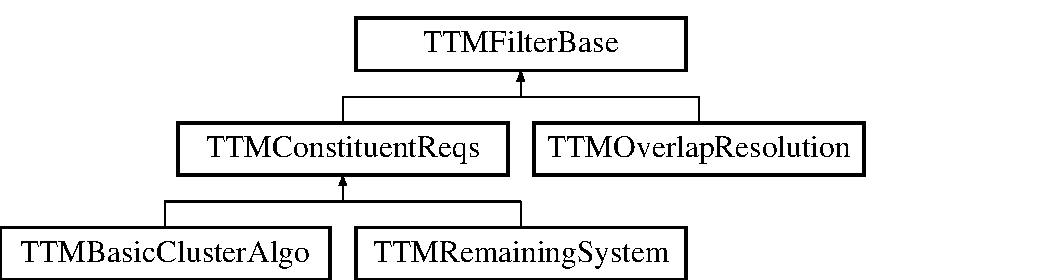
\includegraphics[height=3.000000cm]{classTTMFilterBase}
\end{center}
\end{figure}
\subsection*{Protected Member Functions}
\begin{DoxyCompactItemize}
\item 
bool \hyperlink{classTTMFilterBase_a98fd6161e5b20134fb1b963c182ba630}{constituents\-Are\-Used} (const std\-::vector$<$ const \hyperlink{classConstituent}{Constituent} $\ast$ $>$ \&, const std\-::set$<$ const \hyperlink{classConstituent}{Constituent} $\ast$ $>$ \&, const double, const double) const 
\item 
void \hyperlink{classTTMFilterBase_aaddc805db839d120d018855e4ba12c67}{mark\-Constituents\-Used} (const std\-::vector$<$ const \hyperlink{classConstituent}{Constituent} $\ast$ $>$ \&, const std\-::vector$<$ \hyperlink{classConstituent}{Constituent} $>$ \&, std\-::set$<$ const \hyperlink{classConstituent}{Constituent} $\ast$ $>$ \&, const double, const double) const 
\end{DoxyCompactItemize}


\subsection{Detailed Description}
This class provides several common functions which can be used by \hyperlink{classTTModule}{T\-T\-Module} objects (it is not one itself) to assist in overlap resolution when top candidates sharing the same constituents are selected. 

\subsection{Member Function Documentation}
\hypertarget{classTTMFilterBase_a98fd6161e5b20134fb1b963c182ba630}{\index{T\-T\-M\-Filter\-Base@{T\-T\-M\-Filter\-Base}!constituents\-Are\-Used@{constituents\-Are\-Used}}
\index{constituents\-Are\-Used@{constituents\-Are\-Used}!TTMFilterBase@{T\-T\-M\-Filter\-Base}}
\subsubsection[{constituents\-Are\-Used}]{\setlength{\rightskip}{0pt plus 5cm}bool T\-T\-M\-Filter\-Base\-::constituents\-Are\-Used (
\begin{DoxyParamCaption}
\item[{const std\-::vector$<$ const {\bf Constituent} $\ast$ $>$ \&}]{constituents, }
\item[{const std\-::set$<$ const {\bf Constituent} $\ast$ $>$ \&}]{used\-Consts, }
\item[{const double}]{d\-R\-Max, }
\item[{const double}]{d\-R\-Max\-A\-K8}
\end{DoxyParamCaption}
) const\hspace{0.3cm}{\ttfamily [protected]}}}\label{classTTMFilterBase_a98fd6161e5b20134fb1b963c182ba630}
Checks if the constituents are used


\begin{DoxyParams}{Parameters}
{\em constituents} & List of constituents to check \\
\hline
{\em used\-Consts} & Set of all constituents already used in final reconstructed tops \\
\hline
{\em d\-R\-Match} & The d\-R requirement used to select whether an A\-K4 jet matches a A\-K8 subjet \\
\hline
\end{DoxyParams}
\hypertarget{classTTMFilterBase_aaddc805db839d120d018855e4ba12c67}{\index{T\-T\-M\-Filter\-Base@{T\-T\-M\-Filter\-Base}!mark\-Constituents\-Used@{mark\-Constituents\-Used}}
\index{mark\-Constituents\-Used@{mark\-Constituents\-Used}!TTMFilterBase@{T\-T\-M\-Filter\-Base}}
\subsubsection[{mark\-Constituents\-Used}]{\setlength{\rightskip}{0pt plus 5cm}void T\-T\-M\-Filter\-Base\-::mark\-Constituents\-Used (
\begin{DoxyParamCaption}
\item[{const std\-::vector$<$ const {\bf Constituent} $\ast$ $>$ \&}]{constituents, }
\item[{const std\-::vector$<$ {\bf Constituent} $>$ \&}]{all\-Constituents, }
\item[{std\-::set$<$ const {\bf Constituent} $\ast$ $>$ \&}]{used\-Constituents, }
\item[{const double}]{d\-R\-Max, }
\item[{const double}]{d\-R\-Max\-A\-K8}
\end{DoxyParamCaption}
) const\hspace{0.3cm}{\ttfamily [protected]}}}\label{classTTMFilterBase_aaddc805db839d120d018855e4ba12c67}
Marks constituents as being used in a final reconstructed top


\begin{DoxyParams}{Parameters}
{\em constituents} & List of constituents to mark as used \\
\hline
{\em all\-Constituents} & List of all constituents \\
\hline
{\em used\-Constituents} & Set of all constituents already used in final reconstructed tops \\
\hline
{\em d\-R\-Match} & The d\-R requirement used to select whether an A\-K4 jet matches a A\-K8 subjet \\
\hline
\end{DoxyParams}


The documentation for this class was generated from the following files\-:\begin{DoxyCompactItemize}
\item 
/home/travis/build/susy2015/\-Top\-Tagger/\-Top\-Tagger/include/T\-T\-M\-Filter\-Base.\-h\item 
/home/travis/build/susy2015/\-Top\-Tagger/\-Top\-Tagger/src/T\-T\-M\-Filter\-Base.\-cpp\end{DoxyCompactItemize}

\hypertarget{classTTMFinalSort}{\section{T\-T\-M\-Final\-Sort Class Reference}
\label{classTTMFinalSort}\index{T\-T\-M\-Final\-Sort@{T\-T\-M\-Final\-Sort}}
}


{\ttfamily \#include $<$T\-T\-M\-Final\-Sort.\-h$>$}

Inheritance diagram for T\-T\-M\-Final\-Sort\-:\begin{figure}[H]
\begin{center}
\leavevmode
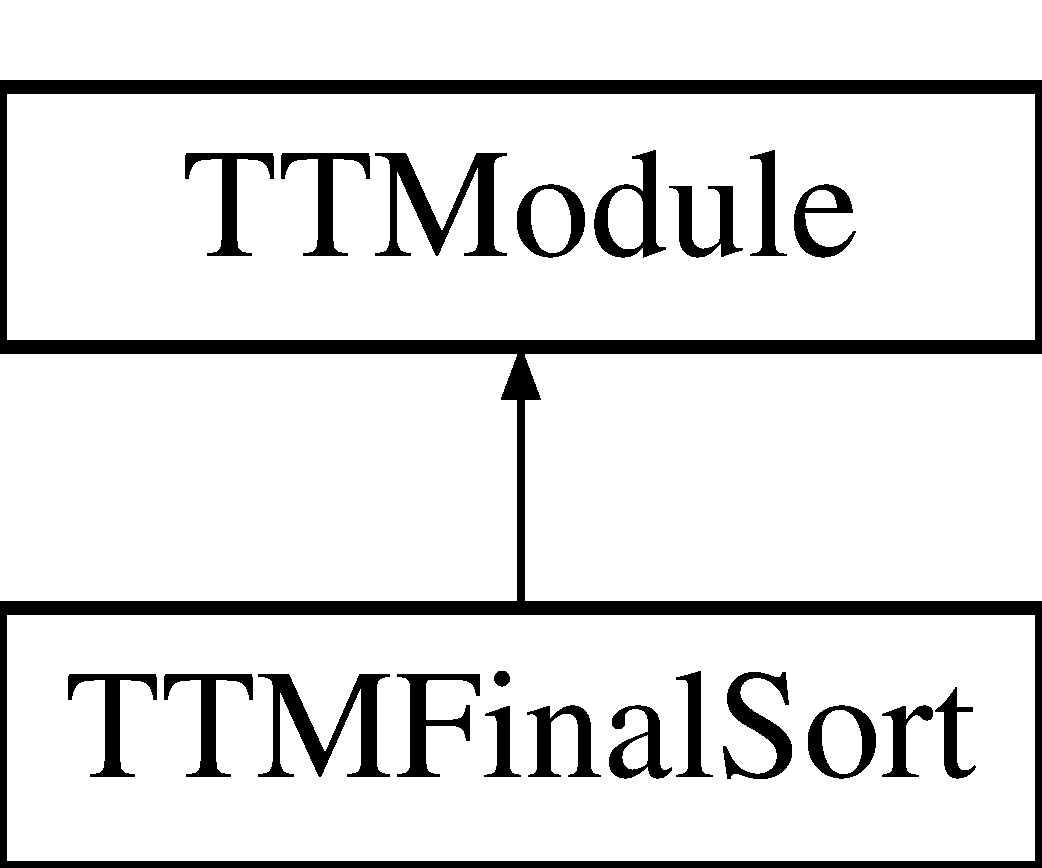
\includegraphics[height=2.000000cm]{classTTMFinalSort}
\end{center}
\end{figure}
\subsection*{Public Member Functions}
\begin{DoxyCompactItemize}
\item 
void \hyperlink{classTTMFinalSort_a1d26fb550c790fb08476c3d4eab99cfd}{get\-Parameters} (const \hyperlink{classcfg_1_1CfgDocument}{cfg\-::\-Cfg\-Document} $\ast$, const std\-::string \&)
\item 
void \hyperlink{classTTMFinalSort_ae4a9797de31364e116fe4b99c57c4afd}{run} (\hyperlink{classTopTaggerResults}{Top\-Tagger\-Results} \&)
\end{DoxyCompactItemize}


\subsection{Detailed Description}
This module is used to sort the final list of tops after overlap resolution.


\begin{DoxyParams}{Parameters}
{\em mt} & (float) {\bfseries  Common context } Mass of the top quark \\
\hline
{\em sort\-Method} & (string) This parameter defines the sorting order. The possible options are \char`\"{}top\-Mass\char`\"{}, \char`\"{}top\-Pt\char`\"{}, and \char`\"{}none\char`\"{}. \\
\hline
\end{DoxyParams}


\subsection{Member Function Documentation}
\hypertarget{classTTMFinalSort_a1d26fb550c790fb08476c3d4eab99cfd}{\index{T\-T\-M\-Final\-Sort@{T\-T\-M\-Final\-Sort}!get\-Parameters@{get\-Parameters}}
\index{get\-Parameters@{get\-Parameters}!TTMFinalSort@{T\-T\-M\-Final\-Sort}}
\subsubsection[{get\-Parameters}]{\setlength{\rightskip}{0pt plus 5cm}void T\-T\-M\-Final\-Sort\-::get\-Parameters (
\begin{DoxyParamCaption}
\item[{const {\bf cfg\-::\-Cfg\-Document} $\ast$}]{, }
\item[{const std\-::string \&}]{}
\end{DoxyParamCaption}
)\hspace{0.3cm}{\ttfamily [virtual]}}}\label{classTTMFinalSort_a1d26fb550c790fb08476c3d4eab99cfd}
This function is called by \hyperlink{classTopTagger}{Top\-Tagger} to configure each module based upon the information present in the configuration file. The inputs for this function are provided by \hyperlink{classTopTagger}{Top\-Tagger} and are the configuration document object and the local context string for this module. The local context string defines where to look in the configuration file for the local parameters. 

Implements \hyperlink{classTTModule_aa9d2842c9e94782059fe92044a68e3a6}{T\-T\-Module}.

\hypertarget{classTTMFinalSort_ae4a9797de31364e116fe4b99c57c4afd}{\index{T\-T\-M\-Final\-Sort@{T\-T\-M\-Final\-Sort}!run@{run}}
\index{run@{run}!TTMFinalSort@{T\-T\-M\-Final\-Sort}}
\subsubsection[{run}]{\setlength{\rightskip}{0pt plus 5cm}void T\-T\-M\-Final\-Sort\-::run (
\begin{DoxyParamCaption}
\item[{{\bf Top\-Tagger\-Results} \&}]{}
\end{DoxyParamCaption}
)\hspace{0.3cm}{\ttfamily [virtual]}}}\label{classTTMFinalSort_ae4a9797de31364e116fe4b99c57c4afd}
run is called automatically by \hyperlink{classTopTagger}{Top\-Tagger} once per event to run th emodule. The module interfaces with other modules through the \hyperlink{classTopTaggerResults}{Top\-Tagger\-Results} object which is passed as a non-\/const reference from \hyperlink{classTopTagger}{Top\-Tagger}. 

Implements \hyperlink{classTTModule_a14e7c03fbf4ee1a5008c9344adc7c896}{T\-T\-Module}.



The documentation for this class was generated from the following files\-:\begin{DoxyCompactItemize}
\item 
/home/travis/build/susy2015/\-Top\-Tagger/\-Top\-Tagger/include/T\-T\-M\-Final\-Sort.\-h\item 
/home/travis/build/susy2015/\-Top\-Tagger/\-Top\-Tagger/src/T\-T\-M\-Final\-Sort.\-cpp\end{DoxyCompactItemize}

\hypertarget{classTTMHEPRequirements}{\section{T\-T\-M\-H\-E\-P\-Requirements Class Reference}
\label{classTTMHEPRequirements}\index{T\-T\-M\-H\-E\-P\-Requirements@{T\-T\-M\-H\-E\-P\-Requirements}}
}


{\ttfamily \#include $<$T\-T\-M\-H\-E\-P\-Requirements.\-h$>$}

Inheritance diagram for T\-T\-M\-H\-E\-P\-Requirements\-:\begin{figure}[H]
\begin{center}
\leavevmode
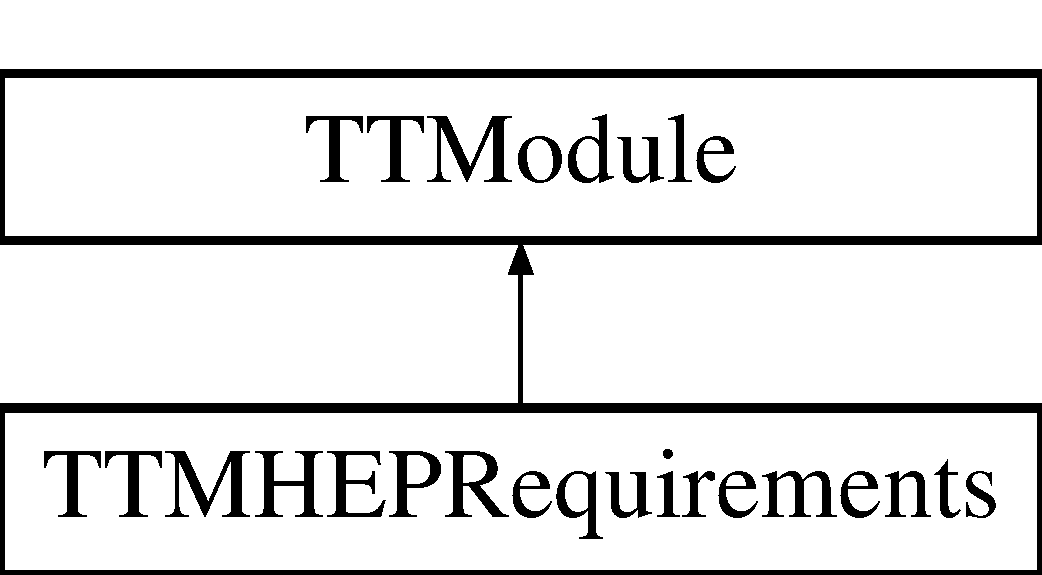
\includegraphics[height=2.000000cm]{classTTMHEPRequirements}
\end{center}
\end{figure}
\subsection*{Public Member Functions}
\begin{DoxyCompactItemize}
\item 
void \hyperlink{classTTMHEPRequirements_ad86f4c8dc3dfc9b2a3925892e9ea82ec}{get\-Parameters} (const \hyperlink{classcfg_1_1CfgDocument}{cfg\-::\-Cfg\-Document} $\ast$, const std\-::string \&)
\item 
void \hyperlink{classTTMHEPRequirements_a5815a6c66595320c1d0f0f006dd67a4d}{run} (\hyperlink{classTopTaggerResults}{Top\-Tagger\-Results} \&)
\end{DoxyCompactItemize}
\subsection*{Additional Inherited Members}


\subsection{Detailed Description}
This module applies the H\-E\-P top tagging criterion to the candidates as well as applying basic requirements on the number of b-\/jets in the candidate. For trijet candidates the full H\-E\-P requirements are applied. For dijet candidates the module applies a simplified version of the H\-E\-P criterion designed for use with a W and an additional jet. The dijet and trijet categories will function with either inputs from \hyperlink{classTTMLazyClusterAlgo}{T\-T\-M\-Lazy\-Cluster\-Algo} or \hyperlink{classTTMBasicClusterAlgo}{T\-T\-M\-Basic\-Cluster\-Algo}. If the monojet mode is activated it will simply pass all A\-K4 monojet top candidates, but not A\-K8 monojet tops (this is instead done by \char`\"{}\-T\-T\-M\-A\-K8\-Top\-Filter\char`\"{}). Candidates passed by this module are placed into the final top list.


\begin{DoxyParams}{Parameters}
{\em Rmin,Rmax} & (float) These parameters define the valid range for the R parameter in the H\-E\-P top tagging requirements. Under the basic assumption that the input jets are massless, this requires that ratio of dijet to trijet masses (inside a jet triplet) is consistent with the ratio of the w to top masses within the specified bounds. This applies to the full trijet H\-E\-P requirements as well as the simplified requirements for the dijet case. \\
\hline
{\em csv\-Threshold} & (float) The minimum cut value on the C\-S\-V discriminator for an A\-K4 jet to be considered a b-\/tagged jet. \\
\hline
{\em b\-Eta\-Cut} & (float) The maximum absolute psudorapidity requirement placed on jets to be considered b-\/tagged. \\
\hline
{\em max\-Nb\-In\-Top} & (integer) The maximum number of b-\/jets to allow in a single top candidate. \\
\hline
{\em do\-Monojet} & (boolean) Enable the processing of A\-K4 monojet top candidates by this module (they are currently all automatically passed by this module). \\
\hline
{\em do\-Dijet} & (boolean) Enable the processing of A\-K4 dijet candidates or A\-K8 W + A\-K4 jet candidates (depending which clustering algorithm is used). \\
\hline
{\em do\-Trijet} & (boolean) Enable the selection criterion for resolved A\-K4 trijet top candidates. \\
\hline
\end{DoxyParams}


\subsection{Member Function Documentation}
\hypertarget{classTTMHEPRequirements_ad86f4c8dc3dfc9b2a3925892e9ea82ec}{\index{T\-T\-M\-H\-E\-P\-Requirements@{T\-T\-M\-H\-E\-P\-Requirements}!get\-Parameters@{get\-Parameters}}
\index{get\-Parameters@{get\-Parameters}!TTMHEPRequirements@{T\-T\-M\-H\-E\-P\-Requirements}}
\subsubsection[{get\-Parameters}]{\setlength{\rightskip}{0pt plus 5cm}void T\-T\-M\-H\-E\-P\-Requirements\-::get\-Parameters (
\begin{DoxyParamCaption}
\item[{const {\bf cfg\-::\-Cfg\-Document} $\ast$}]{, }
\item[{const std\-::string \&}]{}
\end{DoxyParamCaption}
)\hspace{0.3cm}{\ttfamily [virtual]}}}\label{classTTMHEPRequirements_ad86f4c8dc3dfc9b2a3925892e9ea82ec}
This function is called by \hyperlink{classTopTagger}{Top\-Tagger} to configure each module based upon the information present in the configuration file. The inputs for this function are provided by \hyperlink{classTopTagger}{Top\-Tagger} and are the configuration document object and the local context string for this module. The local context string defines where to look in the configuration file for the local parameters. 

Implements \hyperlink{classTTModule_aa9d2842c9e94782059fe92044a68e3a6}{T\-T\-Module}.

\hypertarget{classTTMHEPRequirements_a5815a6c66595320c1d0f0f006dd67a4d}{\index{T\-T\-M\-H\-E\-P\-Requirements@{T\-T\-M\-H\-E\-P\-Requirements}!run@{run}}
\index{run@{run}!TTMHEPRequirements@{T\-T\-M\-H\-E\-P\-Requirements}}
\subsubsection[{run}]{\setlength{\rightskip}{0pt plus 5cm}void T\-T\-M\-H\-E\-P\-Requirements\-::run (
\begin{DoxyParamCaption}
\item[{{\bf Top\-Tagger\-Results} \&}]{}
\end{DoxyParamCaption}
)\hspace{0.3cm}{\ttfamily [virtual]}}}\label{classTTMHEPRequirements_a5815a6c66595320c1d0f0f006dd67a4d}
run is called automatically by \hyperlink{classTopTagger}{Top\-Tagger} once per event to run th emodule. The module interfaces with other modules through the \hyperlink{classTopTaggerResults}{Top\-Tagger\-Results} object which is passed as a non-\/const reference from \hyperlink{classTopTagger}{Top\-Tagger}. 

Implements \hyperlink{classTTModule_a14e7c03fbf4ee1a5008c9344adc7c896}{T\-T\-Module}.



The documentation for this class was generated from the following files\-:\begin{DoxyCompactItemize}
\item 
/home/travis/build/susy2015/\-Top\-Tagger/\-Top\-Tagger/interface/T\-T\-M\-H\-E\-P\-Requirements.\-h\item 
/home/travis/build/susy2015/\-Top\-Tagger/\-Top\-Tagger/src/T\-T\-M\-H\-E\-P\-Requirements.\-cpp\end{DoxyCompactItemize}

\hypertarget{classTTMLazyClusterAlgo}{\section{T\-T\-M\-Lazy\-Cluster\-Algo Class Reference}
\label{classTTMLazyClusterAlgo}\index{T\-T\-M\-Lazy\-Cluster\-Algo@{T\-T\-M\-Lazy\-Cluster\-Algo}}
}
Inheritance diagram for T\-T\-M\-Lazy\-Cluster\-Algo\-:\begin{figure}[H]
\begin{center}
\leavevmode
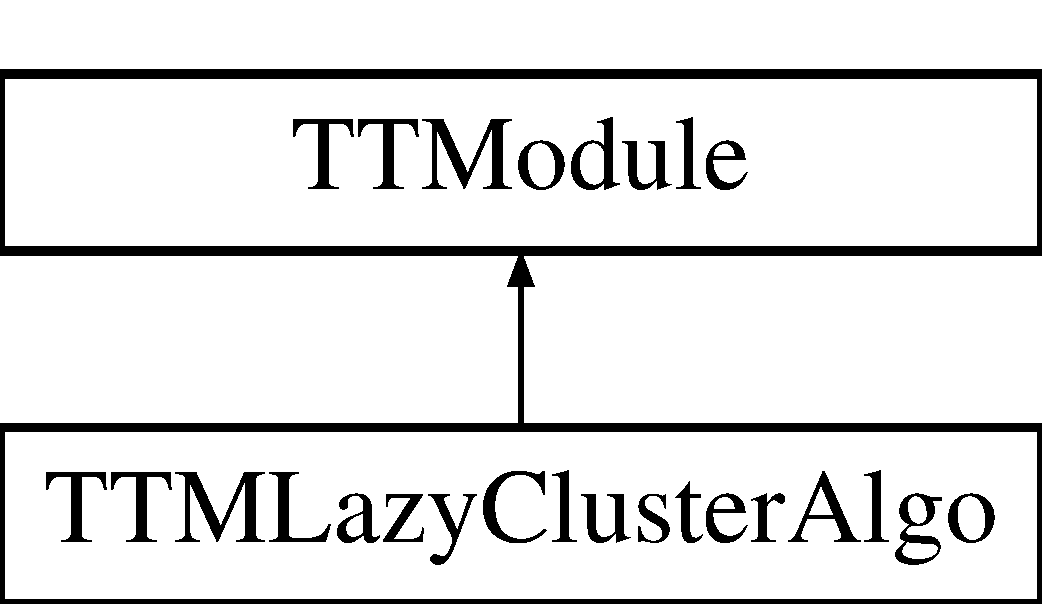
\includegraphics[height=2.000000cm]{classTTMLazyClusterAlgo}
\end{center}
\end{figure}
\subsection*{Public Member Functions}
\begin{DoxyCompactItemize}
\item 
void \hyperlink{classTTMLazyClusterAlgo_a4c07980bb9bc073862bb3b6f7238692c}{get\-Parameters} (const \hyperlink{classcfg_1_1CfgDocument}{cfg\-::\-Cfg\-Document} $\ast$, const std\-::string \&)
\item 
void \hyperlink{classTTMLazyClusterAlgo_a1ec9281c5d6c04ae788b72ca2884d870}{run} (\hyperlink{classTopTaggerResults}{Top\-Tagger\-Results} \&)
\end{DoxyCompactItemize}
\subsection*{Additional Inherited Members}


\subsection{Member Function Documentation}
\hypertarget{classTTMLazyClusterAlgo_a4c07980bb9bc073862bb3b6f7238692c}{\index{T\-T\-M\-Lazy\-Cluster\-Algo@{T\-T\-M\-Lazy\-Cluster\-Algo}!get\-Parameters@{get\-Parameters}}
\index{get\-Parameters@{get\-Parameters}!TTMLazyClusterAlgo@{T\-T\-M\-Lazy\-Cluster\-Algo}}
\subsubsection[{get\-Parameters}]{\setlength{\rightskip}{0pt plus 5cm}void T\-T\-M\-Lazy\-Cluster\-Algo\-::get\-Parameters (
\begin{DoxyParamCaption}
\item[{const {\bf cfg\-::\-Cfg\-Document} $\ast$}]{, }
\item[{const std\-::string \&}]{}
\end{DoxyParamCaption}
)\hspace{0.3cm}{\ttfamily [virtual]}}}\label{classTTMLazyClusterAlgo_a4c07980bb9bc073862bb3b6f7238692c}
This function is called by \hyperlink{classTopTagger}{Top\-Tagger} to configure each module based upon the information present in the configuration file. The inputs for this function are provided by \hyperlink{classTopTagger}{Top\-Tagger} and are the configuration document object and the local context string for this module. The local context string defines where to look in the configuration file for the local parameters. 

Implements \hyperlink{classTTModule_aa9d2842c9e94782059fe92044a68e3a6}{T\-T\-Module}.

\hypertarget{classTTMLazyClusterAlgo_a1ec9281c5d6c04ae788b72ca2884d870}{\index{T\-T\-M\-Lazy\-Cluster\-Algo@{T\-T\-M\-Lazy\-Cluster\-Algo}!run@{run}}
\index{run@{run}!TTMLazyClusterAlgo@{T\-T\-M\-Lazy\-Cluster\-Algo}}
\subsubsection[{run}]{\setlength{\rightskip}{0pt plus 5cm}void T\-T\-M\-Lazy\-Cluster\-Algo\-::run (
\begin{DoxyParamCaption}
\item[{{\bf Top\-Tagger\-Results} \&}]{}
\end{DoxyParamCaption}
)\hspace{0.3cm}{\ttfamily [virtual]}}}\label{classTTMLazyClusterAlgo_a1ec9281c5d6c04ae788b72ca2884d870}
run is called automatically by \hyperlink{classTopTagger}{Top\-Tagger} once per event to run th emodule. The module interfaces with other modules through the \hyperlink{classTopTaggerResults}{Top\-Tagger\-Results} object which is passed as a non-\/const reference from \hyperlink{classTopTagger}{Top\-Tagger}. 

Implements \hyperlink{classTTModule_a14e7c03fbf4ee1a5008c9344adc7c896}{T\-T\-Module}.



The documentation for this class was generated from the following files\-:\begin{DoxyCompactItemize}
\item 
/home/travis/build/susy2015/\-Top\-Tagger/\-Top\-Tagger/include/T\-T\-M\-Lazy\-Cluster\-Algo.\-h\item 
/home/travis/build/susy2015/\-Top\-Tagger/\-Top\-Tagger/src/T\-T\-M\-Lazy\-Cluster\-Algo.\-cpp\end{DoxyCompactItemize}

\hypertarget{classTTMNanoAODClusterAlgo}{\section{T\-T\-M\-Nano\-A\-O\-D\-Cluster\-Algo Class Reference}
\label{classTTMNanoAODClusterAlgo}\index{T\-T\-M\-Nano\-A\-O\-D\-Cluster\-Algo@{T\-T\-M\-Nano\-A\-O\-D\-Cluster\-Algo}}
}


{\ttfamily \#include $<$T\-T\-M\-Nano\-A\-O\-D\-Cluster\-Algo.\-h$>$}

Inheritance diagram for T\-T\-M\-Nano\-A\-O\-D\-Cluster\-Algo\-:\begin{figure}[H]
\begin{center}
\leavevmode
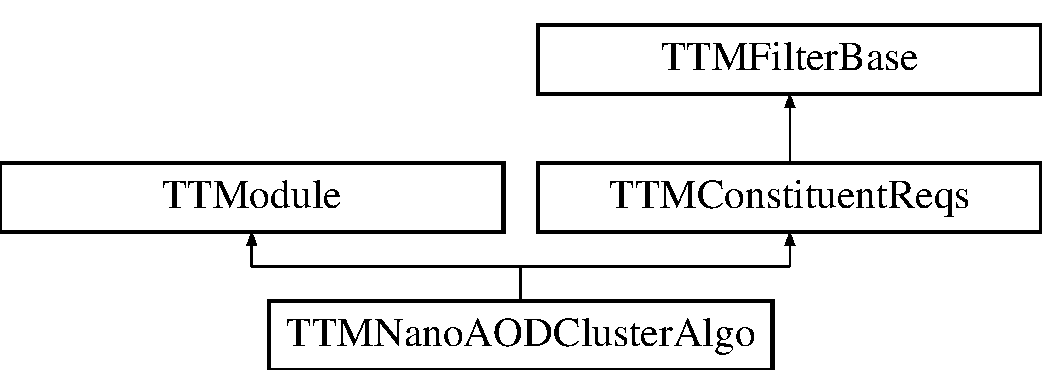
\includegraphics[height=3.000000cm]{classTTMNanoAODClusterAlgo}
\end{center}
\end{figure}
\subsection*{Public Member Functions}
\begin{DoxyCompactItemize}
\item 
void \hyperlink{classTTMNanoAODClusterAlgo_a980b0557cadd8b08953f2fc8f3b26f05}{get\-Parameters} (const \hyperlink{classcfg_1_1CfgDocument}{cfg\-::\-Cfg\-Document} $\ast$, const std\-::string \&)
\item 
void \hyperlink{classTTMNanoAODClusterAlgo_a9885e4ee2ebfe17b5ce9cb86f54830ad}{run} (\hyperlink{classTopTaggerResults}{Top\-Tagger\-Results} \&)
\end{DoxyCompactItemize}
\subsection*{Additional Inherited Members}


\subsection{Detailed Description}
This module is used to cluster top candidates from nano\-A\-O\-D data format. This algorithm assumes that the nano\-A\-O\-D contains all deep\-A\-K8 and deep\-Resolved candidates in the nano\-A\-O\-D already. This module is capable of clustering trijet (resolved tops) and monojet (fully merged top/\-W) candidates.


\begin{DoxyParams}{Parameters}
{\em do\-Trijet} & (bool) Enable the resolved top category clustering. \\
\hline
{\em do\-Monojet} & (bool) Enable the fully merged top category clustering. \\
\hline
{\em do\-Mono\-W} & (bool) Enable the fully merged W category clustering.\\
\hline
\end{DoxyParams}
See \hyperlink{classTTMConstituentReqs}{T\-T\-M\-Constituent\-Reqs} for more parameters 

\subsection{Member Function Documentation}
\hypertarget{classTTMNanoAODClusterAlgo_a980b0557cadd8b08953f2fc8f3b26f05}{\index{T\-T\-M\-Nano\-A\-O\-D\-Cluster\-Algo@{T\-T\-M\-Nano\-A\-O\-D\-Cluster\-Algo}!get\-Parameters@{get\-Parameters}}
\index{get\-Parameters@{get\-Parameters}!TTMNanoAODClusterAlgo@{T\-T\-M\-Nano\-A\-O\-D\-Cluster\-Algo}}
\subsubsection[{get\-Parameters}]{\setlength{\rightskip}{0pt plus 5cm}void T\-T\-M\-Nano\-A\-O\-D\-Cluster\-Algo\-::get\-Parameters (
\begin{DoxyParamCaption}
\item[{const {\bf cfg\-::\-Cfg\-Document} $\ast$}]{, }
\item[{const std\-::string \&}]{}
\end{DoxyParamCaption}
)\hspace{0.3cm}{\ttfamily [virtual]}}}\label{classTTMNanoAODClusterAlgo_a980b0557cadd8b08953f2fc8f3b26f05}
This function is called by \hyperlink{classTopTagger}{Top\-Tagger} to configure each module based upon the information present in the configuration file. The inputs for this function are provided by \hyperlink{classTopTagger}{Top\-Tagger} and are the configuration document object and the local context string for this module. The local context string defines where to look in the configuration file for the local parameters. 

Implements \hyperlink{classTTModule_aa9d2842c9e94782059fe92044a68e3a6}{T\-T\-Module}.

\hypertarget{classTTMNanoAODClusterAlgo_a9885e4ee2ebfe17b5ce9cb86f54830ad}{\index{T\-T\-M\-Nano\-A\-O\-D\-Cluster\-Algo@{T\-T\-M\-Nano\-A\-O\-D\-Cluster\-Algo}!run@{run}}
\index{run@{run}!TTMNanoAODClusterAlgo@{T\-T\-M\-Nano\-A\-O\-D\-Cluster\-Algo}}
\subsubsection[{run}]{\setlength{\rightskip}{0pt plus 5cm}void T\-T\-M\-Nano\-A\-O\-D\-Cluster\-Algo\-::run (
\begin{DoxyParamCaption}
\item[{{\bf Top\-Tagger\-Results} \&}]{}
\end{DoxyParamCaption}
)\hspace{0.3cm}{\ttfamily [virtual]}}}\label{classTTMNanoAODClusterAlgo_a9885e4ee2ebfe17b5ce9cb86f54830ad}
run is called automatically by \hyperlink{classTopTagger}{Top\-Tagger} once per event to run th emodule. The module interfaces with other modules through the \hyperlink{classTopTaggerResults}{Top\-Tagger\-Results} object which is passed as a non-\/const reference from \hyperlink{classTopTagger}{Top\-Tagger}. 

Implements \hyperlink{classTTModule_a14e7c03fbf4ee1a5008c9344adc7c896}{T\-T\-Module}.



The documentation for this class was generated from the following files\-:\begin{DoxyCompactItemize}
\item 
/home/travis/build/susy2015/\-Top\-Tagger/\-Top\-Tagger/interface/T\-T\-M\-Nano\-A\-O\-D\-Cluster\-Algo.\-h\item 
/home/travis/build/susy2015/\-Top\-Tagger/\-Top\-Tagger/src/T\-T\-M\-Nano\-A\-O\-D\-Cluster\-Algo.\-cpp\end{DoxyCompactItemize}

\hypertarget{classTTModule}{\section{T\-T\-Module Class Reference}
\label{classTTModule}\index{T\-T\-Module@{T\-T\-Module}}
}


{\ttfamily \#include $<$T\-T\-Module.\-h$>$}

Inheritance diagram for T\-T\-Module\-:\begin{figure}[H]
\begin{center}
\leavevmode
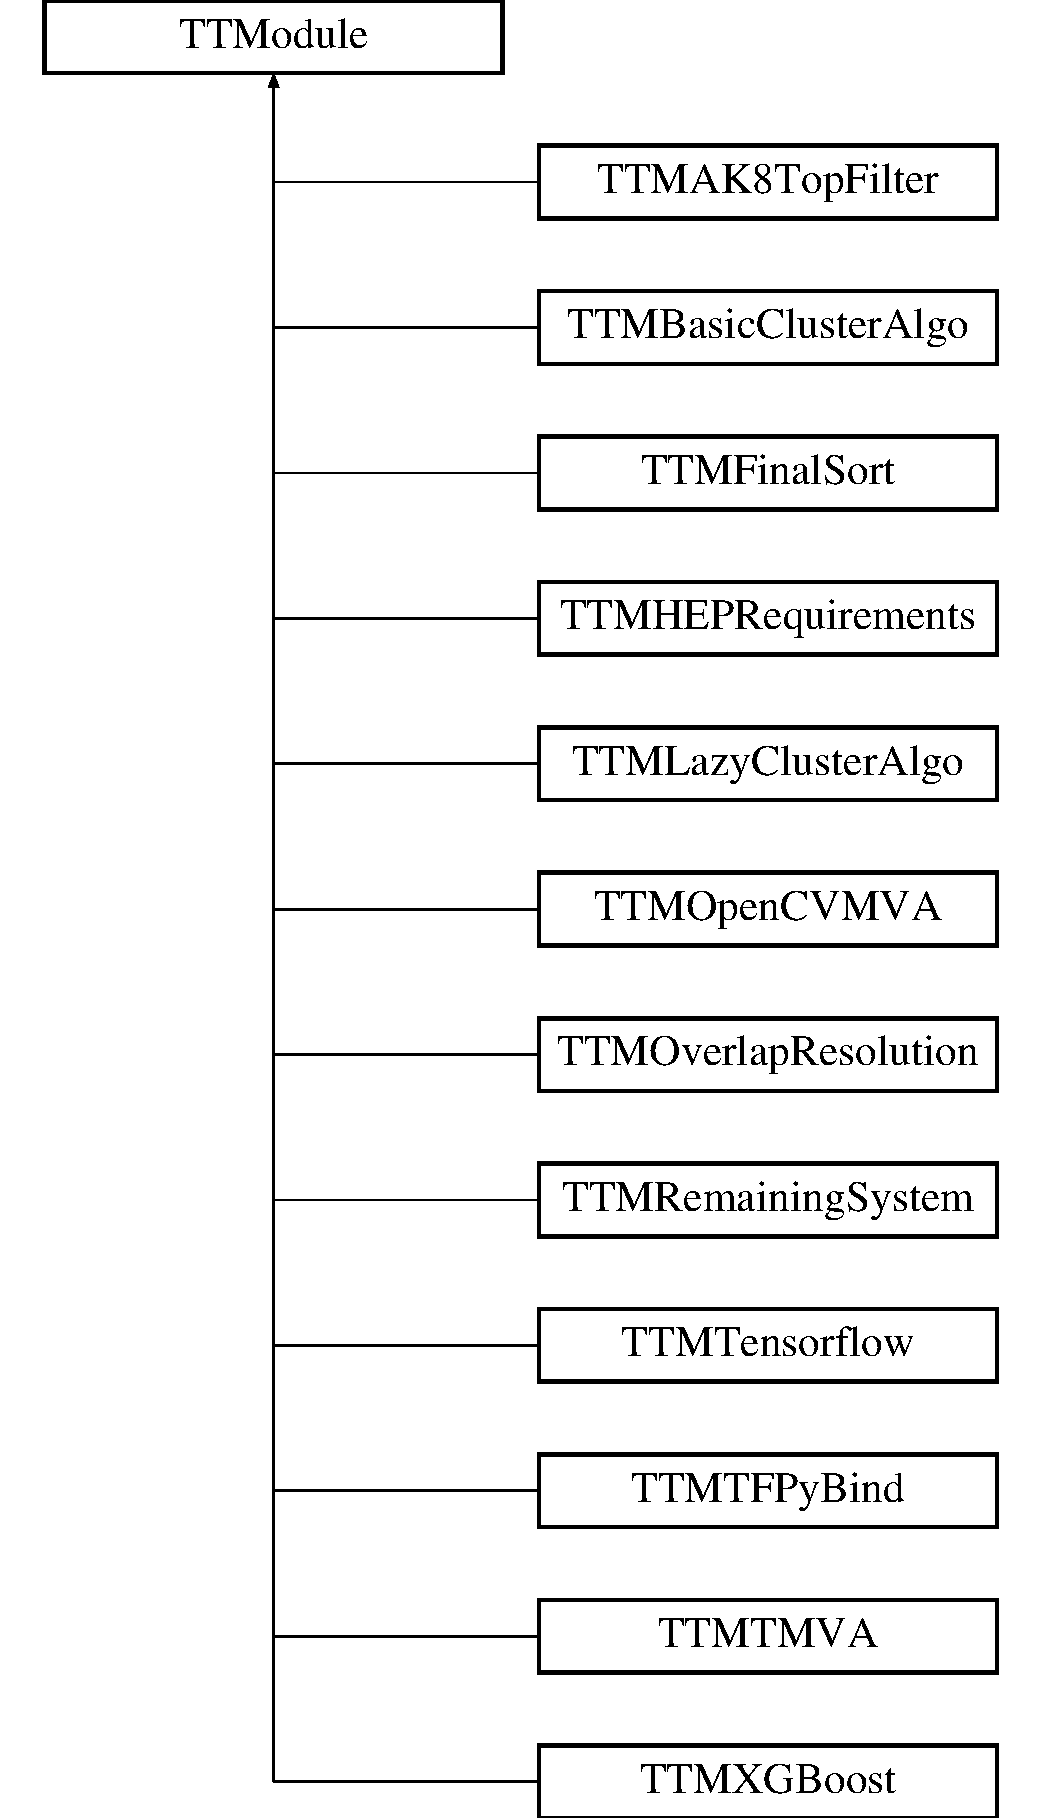
\includegraphics[height=12.000000cm]{classTTModule}
\end{center}
\end{figure}
\subsection*{Public Member Functions}
\begin{DoxyCompactItemize}
\item 
virtual \hyperlink{classTTModule_a270f4faaa37f3fb382fb5fa91cdf1899}{$\sim$\-T\-T\-Module} ()=default
\item 
virtual void \hyperlink{classTTModule_aa9d2842c9e94782059fe92044a68e3a6}{get\-Parameters} (const \hyperlink{classcfg_1_1CfgDocument}{cfg\-::\-Cfg\-Document} $\ast$, const std\-::string \&)=0
\item 
virtual void \hyperlink{classTTModule_a14e7c03fbf4ee1a5008c9344adc7c896}{run} (\hyperlink{classTopTaggerResults}{Top\-Tagger\-Results} \&)=0
\item 
void \hyperlink{classTTModule_a0f9c9948826e630e6c6e7943e98a1f37}{set\-Working\-Directory} (const std\-::string \&working\-Dir)
\end{DoxyCompactItemize}
\subsection*{Protected Attributes}
\begin{DoxyCompactItemize}
\item 
\hypertarget{classTTModule_a7ef21f981480be1787d2d606023fafd8}{std\-::string \hyperlink{classTTModule_a7ef21f981480be1787d2d606023fafd8}{working\-Directory\-\_\-}}\label{classTTModule_a7ef21f981480be1787d2d606023fafd8}

\begin{DoxyCompactList}\small\item\em Stores the location where the tagger will resolve relative file paths. \end{DoxyCompactList}\end{DoxyCompactItemize}


\subsection{Detailed Description}
This is a pure virtual base class which defines the interface for a top tagger module. This implements 2 pure virtual functions which must be overridden by all modules. The first, \char`\"{}get\-Parameters,\char`\"{} is used to load any configuration parameters the module may need from the config file. The second, \char`\"{}run,\char`\"{} is used to run the particular algorithm implemented in the module. None of these functions should even be called directly, but instead are called automatically by the \hyperlink{classTopTagger}{Top\-Tagger} class. It is also important that each module also include the line \char`\"{}\-R\-E\-G\-E\-S\-T\-E\-R\-\_\-\-T\-T\-M\-O\-D\-U\-L\-E(\-Module\-Class\-Name)\char`\"{} after the class declaration. This macro calls special code so that the \hyperlink{classTTMFactory}{T\-T\-M\-Factory} class can dynamically implement the module by name. 

\subsection{Constructor \& Destructor Documentation}
\hypertarget{classTTModule_a270f4faaa37f3fb382fb5fa91cdf1899}{\index{T\-T\-Module@{T\-T\-Module}!$\sim$\-T\-T\-Module@{$\sim$\-T\-T\-Module}}
\index{$\sim$\-T\-T\-Module@{$\sim$\-T\-T\-Module}!TTModule@{T\-T\-Module}}
\subsubsection[{$\sim$\-T\-T\-Module}]{\setlength{\rightskip}{0pt plus 5cm}virtual T\-T\-Module\-::$\sim$\-T\-T\-Module (
\begin{DoxyParamCaption}
{}
\end{DoxyParamCaption}
)\hspace{0.3cm}{\ttfamily [virtual]}, {\ttfamily [default]}}}\label{classTTModule_a270f4faaa37f3fb382fb5fa91cdf1899}
Virtual base distructor in case other daughter classes need distructors 

\subsection{Member Function Documentation}
\hypertarget{classTTModule_aa9d2842c9e94782059fe92044a68e3a6}{\index{T\-T\-Module@{T\-T\-Module}!get\-Parameters@{get\-Parameters}}
\index{get\-Parameters@{get\-Parameters}!TTModule@{T\-T\-Module}}
\subsubsection[{get\-Parameters}]{\setlength{\rightskip}{0pt plus 5cm}virtual void T\-T\-Module\-::get\-Parameters (
\begin{DoxyParamCaption}
\item[{const {\bf cfg\-::\-Cfg\-Document} $\ast$}]{, }
\item[{const std\-::string \&}]{}
\end{DoxyParamCaption}
)\hspace{0.3cm}{\ttfamily [pure virtual]}}}\label{classTTModule_aa9d2842c9e94782059fe92044a68e3a6}
This function is called by \hyperlink{classTopTagger}{Top\-Tagger} to configure each module based upon the information present in the configuration file. The inputs for this function are provided by \hyperlink{classTopTagger}{Top\-Tagger} and are the configuration document object and the local context string for this module. The local context string defines where to look in the configuration file for the local parameters. 

Implemented in \hyperlink{classTTMTensorflow_ae8a95bbecd4a21698b64dc95e99f5f0f}{T\-T\-M\-Tensorflow}, \hyperlink{classTTMTFPyBind_a3c9f2ca6bc095df3bad89c531cd45544}{T\-T\-M\-T\-F\-Py\-Bind}, \hyperlink{classTTMXGBoost_a852aba8afb6f453187871e232927e622}{T\-T\-M\-X\-G\-Boost}, \hyperlink{classTTMBasicClusterAlgo_afdbe472d26a753268dac63d897169299}{T\-T\-M\-Basic\-Cluster\-Algo}, \hyperlink{classTTMTMVA_a00b1eda9a6425e95eb4e0f41688236e0}{T\-T\-M\-T\-M\-V\-A}, \hyperlink{classTTMOpenCVMVA_a9842e490d60a486958ba93b6f0f5d00e}{T\-T\-M\-Open\-C\-V\-M\-V\-A}, \hyperlink{classTTMOverlapResolution_a4dd88bd8480301018cfba596ae226157}{T\-T\-M\-Overlap\-Resolution}, \hyperlink{classTTMHEPRequirements_ad86f4c8dc3dfc9b2a3925892e9ea82ec}{T\-T\-M\-H\-E\-P\-Requirements}, \hyperlink{classTTMFinalSort_a1d26fb550c790fb08476c3d4eab99cfd}{T\-T\-M\-Final\-Sort}, \hyperlink{classTTMRemainingSystem_a4d72b9607c336e2de3d2f7876c89f5db}{T\-T\-M\-Remaining\-System}, \hyperlink{classTTMAK8TopFilter_aed52bd6877ec9b8ac3a2f45769f05856}{T\-T\-M\-A\-K8\-Top\-Filter}, and \hyperlink{classTTMLazyClusterAlgo_a4c07980bb9bc073862bb3b6f7238692c}{T\-T\-M\-Lazy\-Cluster\-Algo}.

\hypertarget{classTTModule_a14e7c03fbf4ee1a5008c9344adc7c896}{\index{T\-T\-Module@{T\-T\-Module}!run@{run}}
\index{run@{run}!TTModule@{T\-T\-Module}}
\subsubsection[{run}]{\setlength{\rightskip}{0pt plus 5cm}virtual void T\-T\-Module\-::run (
\begin{DoxyParamCaption}
\item[{{\bf Top\-Tagger\-Results} \&}]{}
\end{DoxyParamCaption}
)\hspace{0.3cm}{\ttfamily [pure virtual]}}}\label{classTTModule_a14e7c03fbf4ee1a5008c9344adc7c896}
run is called automatically by \hyperlink{classTopTagger}{Top\-Tagger} once per event to run th emodule. The module interfaces with other modules through the \hyperlink{classTopTaggerResults}{Top\-Tagger\-Results} object which is passed as a non-\/const reference from \hyperlink{classTopTagger}{Top\-Tagger}. 

Implemented in \hyperlink{classTTMTensorflow_afe5cdab757948e8eb2713fab0385869b}{T\-T\-M\-Tensorflow}, \hyperlink{classTTMTFPyBind_a5815a77655f5500c117cf71269105242}{T\-T\-M\-T\-F\-Py\-Bind}, \hyperlink{classTTMXGBoost_afd522be937c0e1c8226c83cc6888c666}{T\-T\-M\-X\-G\-Boost}, \hyperlink{classTTMBasicClusterAlgo_ae1d464bf1db5762318766d109c843932}{T\-T\-M\-Basic\-Cluster\-Algo}, \hyperlink{classTTMTMVA_a640584674f072cb893685845080c5eb9}{T\-T\-M\-T\-M\-V\-A}, \hyperlink{classTTMOpenCVMVA_af51d1bf351304ef8c6e732763d58c433}{T\-T\-M\-Open\-C\-V\-M\-V\-A}, \hyperlink{classTTMOverlapResolution_a4099ee72e105acbcca10078068775bef}{T\-T\-M\-Overlap\-Resolution}, \hyperlink{classTTMHEPRequirements_a5815a6c66595320c1d0f0f006dd67a4d}{T\-T\-M\-H\-E\-P\-Requirements}, \hyperlink{classTTMFinalSort_ae4a9797de31364e116fe4b99c57c4afd}{T\-T\-M\-Final\-Sort}, \hyperlink{classTTMRemainingSystem_ab9f2abe56c30f34c2319f752c403fb09}{T\-T\-M\-Remaining\-System}, \hyperlink{classTTMAK8TopFilter_a28a8fcd8a829caae32b2a106037d3a6f}{T\-T\-M\-A\-K8\-Top\-Filter}, and \hyperlink{classTTMLazyClusterAlgo_a1ec9281c5d6c04ae788b72ca2884d870}{T\-T\-M\-Lazy\-Cluster\-Algo}.

\hypertarget{classTTModule_a0f9c9948826e630e6c6e7943e98a1f37}{\index{T\-T\-Module@{T\-T\-Module}!set\-Working\-Directory@{set\-Working\-Directory}}
\index{set\-Working\-Directory@{set\-Working\-Directory}!TTModule@{T\-T\-Module}}
\subsubsection[{set\-Working\-Directory}]{\setlength{\rightskip}{0pt plus 5cm}void T\-T\-Module\-::set\-Working\-Directory (
\begin{DoxyParamCaption}
\item[{const std\-::string \&}]{working\-Dir}
\end{DoxyParamCaption}
)\hspace{0.3cm}{\ttfamily [inline]}}}\label{classTTModule_a0f9c9948826e630e6c6e7943e98a1f37}
This function sets the base directory from which all files accessed through relative paths should be referenced 

The documentation for this class was generated from the following file\-:\begin{DoxyCompactItemize}
\item 
/home/travis/build/susy2015/\-Top\-Tagger/\-Top\-Tagger/include/\hyperlink{TTModule_8h}{T\-T\-Module.\-h}\end{DoxyCompactItemize}

\hypertarget{classTTMOpenCVMVA}{\section{T\-T\-M\-Open\-C\-V\-M\-V\-A Class Reference}
\label{classTTMOpenCVMVA}\index{T\-T\-M\-Open\-C\-V\-M\-V\-A@{T\-T\-M\-Open\-C\-V\-M\-V\-A}}
}


{\ttfamily \#include $<$T\-T\-M\-Open\-C\-V\-M\-V\-A.\-h$>$}

Inheritance diagram for T\-T\-M\-Open\-C\-V\-M\-V\-A\-:\begin{figure}[H]
\begin{center}
\leavevmode
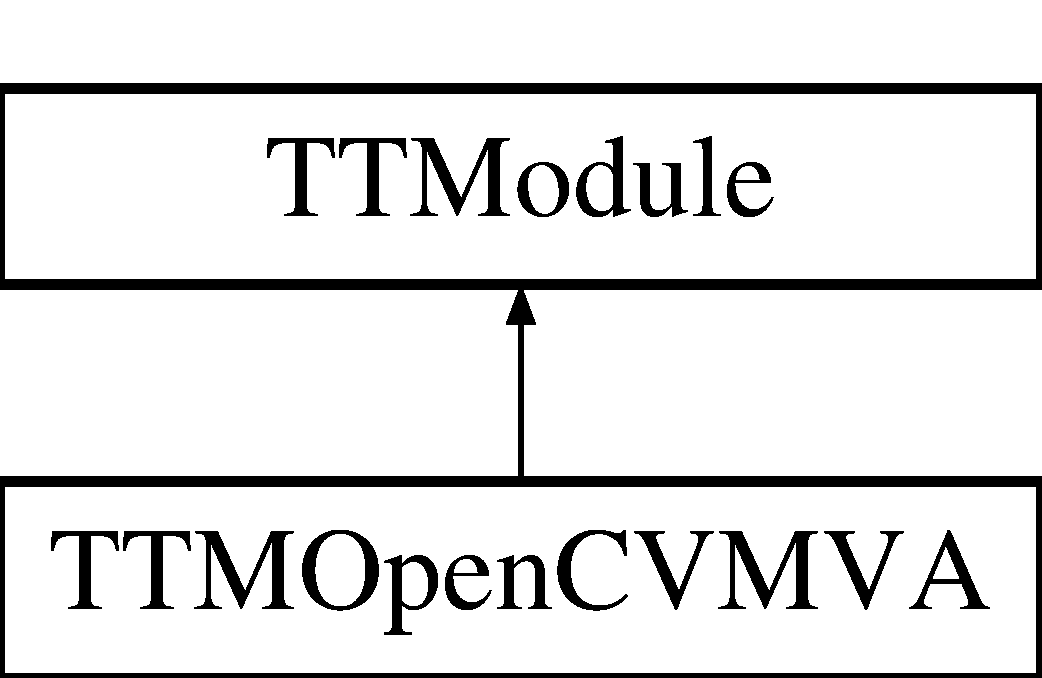
\includegraphics[height=2.000000cm]{classTTMOpenCVMVA}
\end{center}
\end{figure}
\subsection*{Public Member Functions}
\begin{DoxyCompactItemize}
\item 
void \hyperlink{classTTMOpenCVMVA_a9842e490d60a486958ba93b6f0f5d00e}{get\-Parameters} (const \hyperlink{classcfg_1_1CfgDocument}{cfg\-::\-Cfg\-Document} $\ast$, const std\-::string \&)
\item 
void \hyperlink{classTTMOpenCVMVA_af51d1bf351304ef8c6e732763d58c433}{run} (\hyperlink{classTopTaggerResults}{Top\-Tagger\-Results} \&)
\end{DoxyCompactItemize}
\subsection*{Additional Inherited Members}


\subsection{Detailed Description}
This module implements an interface to the Open\-C\-V randomforest package for filtering top candidates. This module can either pass entries directly into the final top list, or filter entries out of the final top list if they do not pass the selection criteria.


\begin{DoxyParams}{Parameters}
{\em disc\-Cut} & (float) Minimum threshold for the T\-M\-V\-A discriminator for the candidate to pass the selection \\
\hline
{\em model\-File} & (string) Path to the model file \\
\hline
{\em csv\-Threshold} & (float) Threshold on b-\/tag discriminator to be considered a b-\/jet. \\
\hline
{\em b\-Eta\-Cut} & (float) Requirment on $\vert$eta$\vert$ for a constituent to be considered a b-\/jet \\
\hline
{\em max\-Nb\-In\-Top} & (int) The maximum number of constituent jets which can be b-\/tagged for the candidate to be a final $\ast$\\
\hline
{\em mva\-Var\mbox{[}$\,$\mbox{]}} & (string -\/ array) M\-V\-A variable input names \\
\hline
\end{DoxyParams}


\subsection{Member Function Documentation}
\hypertarget{classTTMOpenCVMVA_a9842e490d60a486958ba93b6f0f5d00e}{\index{T\-T\-M\-Open\-C\-V\-M\-V\-A@{T\-T\-M\-Open\-C\-V\-M\-V\-A}!get\-Parameters@{get\-Parameters}}
\index{get\-Parameters@{get\-Parameters}!TTMOpenCVMVA@{T\-T\-M\-Open\-C\-V\-M\-V\-A}}
\subsubsection[{get\-Parameters}]{\setlength{\rightskip}{0pt plus 5cm}void T\-T\-M\-Open\-C\-V\-M\-V\-A\-::get\-Parameters (
\begin{DoxyParamCaption}
\item[{const {\bf cfg\-::\-Cfg\-Document} $\ast$}]{, }
\item[{const std\-::string \&}]{}
\end{DoxyParamCaption}
)\hspace{0.3cm}{\ttfamily [virtual]}}}\label{classTTMOpenCVMVA_a9842e490d60a486958ba93b6f0f5d00e}
This function is called by \hyperlink{classTopTagger}{Top\-Tagger} to configure each module based upon the information present in the configuration file. The inputs for this function are provided by \hyperlink{classTopTagger}{Top\-Tagger} and are the configuration document object and the local context string for this module. The local context string defines where to look in the configuration file for the local parameters. 

Implements \hyperlink{classTTModule_aa9d2842c9e94782059fe92044a68e3a6}{T\-T\-Module}.

\hypertarget{classTTMOpenCVMVA_af51d1bf351304ef8c6e732763d58c433}{\index{T\-T\-M\-Open\-C\-V\-M\-V\-A@{T\-T\-M\-Open\-C\-V\-M\-V\-A}!run@{run}}
\index{run@{run}!TTMOpenCVMVA@{T\-T\-M\-Open\-C\-V\-M\-V\-A}}
\subsubsection[{run}]{\setlength{\rightskip}{0pt plus 5cm}void T\-T\-M\-Open\-C\-V\-M\-V\-A\-::run (
\begin{DoxyParamCaption}
\item[{{\bf Top\-Tagger\-Results} \&}]{}
\end{DoxyParamCaption}
)\hspace{0.3cm}{\ttfamily [virtual]}}}\label{classTTMOpenCVMVA_af51d1bf351304ef8c6e732763d58c433}
run is called automatically by \hyperlink{classTopTagger}{Top\-Tagger} once per event to run th emodule. The module interfaces with other modules through the \hyperlink{classTopTaggerResults}{Top\-Tagger\-Results} object which is passed as a non-\/const reference from \hyperlink{classTopTagger}{Top\-Tagger}. 

Implements \hyperlink{classTTModule_a14e7c03fbf4ee1a5008c9344adc7c896}{T\-T\-Module}.



The documentation for this class was generated from the following files\-:\begin{DoxyCompactItemize}
\item 
/home/travis/build/susy2015/\-Top\-Tagger/\-Top\-Tagger/interface/T\-T\-M\-Open\-C\-V\-M\-V\-A.\-h\item 
/home/travis/build/susy2015/\-Top\-Tagger/\-Top\-Tagger/src/T\-T\-M\-Open\-C\-V\-M\-V\-A.\-cpp\end{DoxyCompactItemize}

\hypertarget{classTTMOverlapResolution}{\section{T\-T\-M\-Overlap\-Resolution Class Reference}
\label{classTTMOverlapResolution}\index{T\-T\-M\-Overlap\-Resolution@{T\-T\-M\-Overlap\-Resolution}}
}


{\ttfamily \#include $<$T\-T\-M\-Overlap\-Resolution.\-h$>$}

Inheritance diagram for T\-T\-M\-Overlap\-Resolution\-:\begin{figure}[H]
\begin{center}
\leavevmode
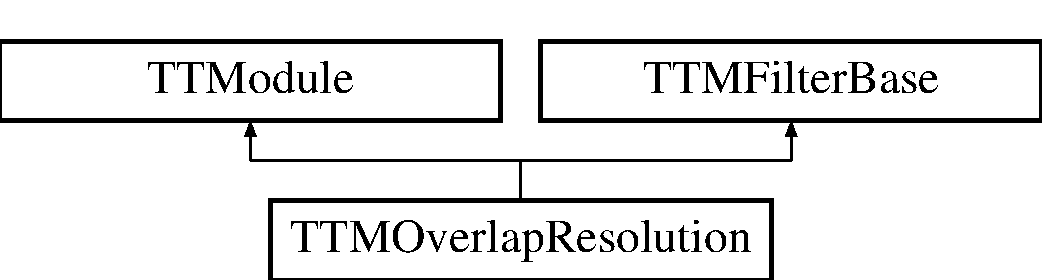
\includegraphics[height=2.000000cm]{classTTMOverlapResolution}
\end{center}
\end{figure}
\subsection*{Public Member Functions}
\begin{DoxyCompactItemize}
\item 
void \hyperlink{classTTMOverlapResolution_a4dd88bd8480301018cfba596ae226157}{get\-Parameters} (const \hyperlink{classcfg_1_1CfgDocument}{cfg\-::\-Cfg\-Document} $\ast$, const std\-::string \&)
\item 
void \hyperlink{classTTMOverlapResolution_a4099ee72e105acbcca10078068775bef}{run} (\hyperlink{classTopTaggerResults}{Top\-Tagger\-Results} \&)
\end{DoxyCompactItemize}
\subsection*{Additional Inherited Members}


\subsection{Detailed Description}
After top candidates are added to the final top list it is possible that some constituent jets can be included in more than one top in the list. This module is used to remove the tops which share constituents. It functions by first sorting the list of tops by a figure of merit, and then in the case that 2 tops share a constituent, the top with the better figure of merit is removed. The module can by run on the entire list of tops, or it can be run category by category.


\begin{DoxyParams}{Parameters}
{\em mt} & (float) {\bfseries  Common context } Mass of the top quark \\
\hline
{\em max\-Top\-Eta} & (float) {\bfseries  Common context } Maximum $\vert$eta$\vert$ of a top candidate to be considered a final reconstructed top \\
\hline
{\em d\-R\-Match} & (float) {\bfseries  Common context } The d\-R requirement used to select whether an A\-K4 jet matches a A\-K8 subjet \\
\hline
{\em cvs\-Threshold} & (float) Minimum cut value on the C\-S\-V discriminator for an A\-K4 jet to be considered a b-\/tagged jet \\
\hline
{\em N\-Constituents} & (int) This parameter determines which tops to include in the overlap resolution process. The options include \char`\"{}-\/1\char`\"{} for all tops, or 1, 2, or 3, for monojet, dijet, or trijet categories respectively. \\
\hline
{\em sort\-Method} & (string) The initial sorting order used to prioritize one top over another when resolving overlapping. The options include \char`\"{}top\-Mass\char`\"{}, \char`\"{}top\-Pt\char`\"{}, \char`\"{}mva\-Disc\char`\"{}, \char`\"{}mva\-Disc\-Withb\char`\"{}, and \char`\"{}none\char`\"{}. \\
\hline
\end{DoxyParams}


\subsection{Member Function Documentation}
\hypertarget{classTTMOverlapResolution_a4dd88bd8480301018cfba596ae226157}{\index{T\-T\-M\-Overlap\-Resolution@{T\-T\-M\-Overlap\-Resolution}!get\-Parameters@{get\-Parameters}}
\index{get\-Parameters@{get\-Parameters}!TTMOverlapResolution@{T\-T\-M\-Overlap\-Resolution}}
\subsubsection[{get\-Parameters}]{\setlength{\rightskip}{0pt plus 5cm}void T\-T\-M\-Overlap\-Resolution\-::get\-Parameters (
\begin{DoxyParamCaption}
\item[{const {\bf cfg\-::\-Cfg\-Document} $\ast$}]{, }
\item[{const std\-::string \&}]{}
\end{DoxyParamCaption}
)\hspace{0.3cm}{\ttfamily [virtual]}}}\label{classTTMOverlapResolution_a4dd88bd8480301018cfba596ae226157}
This function is called by \hyperlink{classTopTagger}{Top\-Tagger} to configure each module based upon the information present in the configuration file. The inputs for this function are provided by \hyperlink{classTopTagger}{Top\-Tagger} and are the configuration document object and the local context string for this module. The local context string defines where to look in the configuration file for the local parameters. 

Implements \hyperlink{classTTModule_aa9d2842c9e94782059fe92044a68e3a6}{T\-T\-Module}.

\hypertarget{classTTMOverlapResolution_a4099ee72e105acbcca10078068775bef}{\index{T\-T\-M\-Overlap\-Resolution@{T\-T\-M\-Overlap\-Resolution}!run@{run}}
\index{run@{run}!TTMOverlapResolution@{T\-T\-M\-Overlap\-Resolution}}
\subsubsection[{run}]{\setlength{\rightskip}{0pt plus 5cm}void T\-T\-M\-Overlap\-Resolution\-::run (
\begin{DoxyParamCaption}
\item[{{\bf Top\-Tagger\-Results} \&}]{}
\end{DoxyParamCaption}
)\hspace{0.3cm}{\ttfamily [virtual]}}}\label{classTTMOverlapResolution_a4099ee72e105acbcca10078068775bef}
run is called automatically by \hyperlink{classTopTagger}{Top\-Tagger} once per event to run th emodule. The module interfaces with other modules through the \hyperlink{classTopTaggerResults}{Top\-Tagger\-Results} object which is passed as a non-\/const reference from \hyperlink{classTopTagger}{Top\-Tagger}. 

Implements \hyperlink{classTTModule_a14e7c03fbf4ee1a5008c9344adc7c896}{T\-T\-Module}.



The documentation for this class was generated from the following files\-:\begin{DoxyCompactItemize}
\item 
/home/travis/build/susy2015/\-Top\-Tagger/\-Top\-Tagger/include/T\-T\-M\-Overlap\-Resolution.\-h\item 
/home/travis/build/susy2015/\-Top\-Tagger/\-Top\-Tagger/src/T\-T\-M\-Overlap\-Resolution.\-cpp\end{DoxyCompactItemize}

\hypertarget{classTTMRemainingSystem}{\section{T\-T\-M\-Remaining\-System Class Reference}
\label{classTTMRemainingSystem}\index{T\-T\-M\-Remaining\-System@{T\-T\-M\-Remaining\-System}}
}


{\ttfamily \#include $<$T\-T\-M\-Remaining\-System.\-h$>$}

Inheritance diagram for T\-T\-M\-Remaining\-System\-:\begin{figure}[H]
\begin{center}
\leavevmode
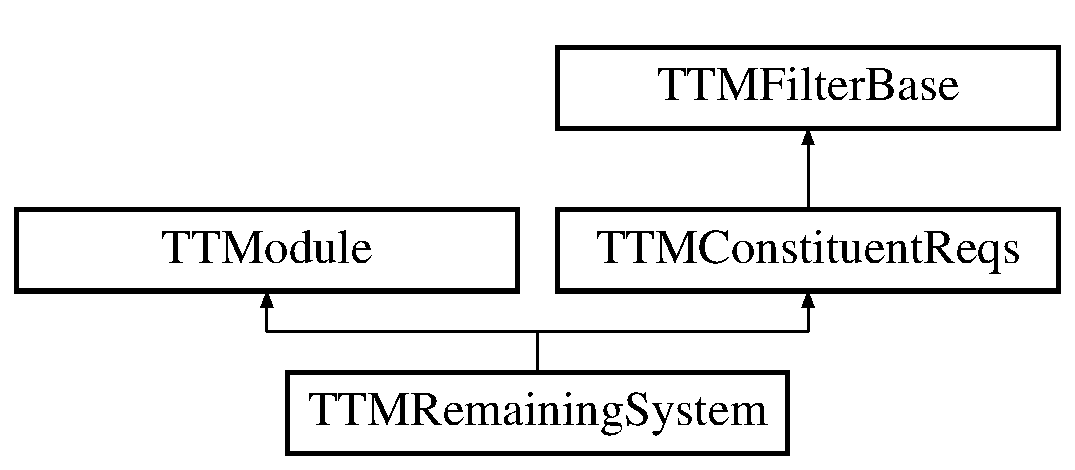
\includegraphics[height=3.000000cm]{classTTMRemainingSystem}
\end{center}
\end{figure}
\subsection*{Public Member Functions}
\begin{DoxyCompactItemize}
\item 
void \hyperlink{classTTMRemainingSystem_a4d72b9607c336e2de3d2f7876c89f5db}{get\-Parameters} (const \hyperlink{classcfg_1_1CfgDocument}{cfg\-::\-Cfg\-Document} $\ast$, const std\-::string \&)
\item 
void \hyperlink{classTTMRemainingSystem_ab9f2abe56c30f34c2319f752c403fb09}{run} (\hyperlink{classTopTaggerResults}{Top\-Tagger\-Results} \&)
\end{DoxyCompactItemize}
\subsection*{Additional Inherited Members}


\subsection{Detailed Description}
This module calclates the remaining system. The purpose of the remaining system is to partially reconstruct a top quark to give a second input into the M\-T2 calculation for the 1-\/top catagory. The reconstruction algorithm used here starts by looking for a b-\/jet not included in a top. If no b jet is found then the highest pt jet not in a top is selected. The algorithm can then combine nearby jets with the first selected jet if certain requirements are satisified. If no second jet satisifies these requirments, the fist chosen jet is used by itself. This algorithm only finds one such object using this method. If multiple jet pairings satisify the requirements, the pairing with the smallest d\-R is chosen.


\begin{DoxyParams}{Parameters}
{\em csv\-Threshold} & (float) Threshold on b-\/tag discriminator to be considered a b-\/jet \\
\hline
{\em low\-Rsys\-Mass} & (float) Lower limit on the mass of the remaining system \\
\hline
{\em high\-Rsys\-Mass} & (float) Upper limit on the mass of the remaining system \\
\hline
{\em d\-R\-Max\-Rsys} & (float) Maximum allowed seperation in d\-R between the jets of the remaining system and their centroid \\
\hline
{\em use\-Second\-Jet} & (bool) Sets whether the algorithm will look for a second jet to combine with the seed jet \\
\hline
{\em allow\-W} & (bool) Sets whether a A\-K8\-W candidate can be a seed for the remaining system \\
\hline
\end{DoxyParams}


\subsection{Member Function Documentation}
\hypertarget{classTTMRemainingSystem_a4d72b9607c336e2de3d2f7876c89f5db}{\index{T\-T\-M\-Remaining\-System@{T\-T\-M\-Remaining\-System}!get\-Parameters@{get\-Parameters}}
\index{get\-Parameters@{get\-Parameters}!TTMRemainingSystem@{T\-T\-M\-Remaining\-System}}
\subsubsection[{get\-Parameters}]{\setlength{\rightskip}{0pt plus 5cm}void T\-T\-M\-Remaining\-System\-::get\-Parameters (
\begin{DoxyParamCaption}
\item[{const {\bf cfg\-::\-Cfg\-Document} $\ast$}]{, }
\item[{const std\-::string \&}]{}
\end{DoxyParamCaption}
)\hspace{0.3cm}{\ttfamily [virtual]}}}\label{classTTMRemainingSystem_a4d72b9607c336e2de3d2f7876c89f5db}
This function is called by \hyperlink{classTopTagger}{Top\-Tagger} to configure each module based upon the information present in the configuration file. The inputs for this function are provided by \hyperlink{classTopTagger}{Top\-Tagger} and are the configuration document object and the local context string for this module. The local context string defines where to look in the configuration file for the local parameters. 

Implements \hyperlink{classTTModule_aa9d2842c9e94782059fe92044a68e3a6}{T\-T\-Module}.

\hypertarget{classTTMRemainingSystem_ab9f2abe56c30f34c2319f752c403fb09}{\index{T\-T\-M\-Remaining\-System@{T\-T\-M\-Remaining\-System}!run@{run}}
\index{run@{run}!TTMRemainingSystem@{T\-T\-M\-Remaining\-System}}
\subsubsection[{run}]{\setlength{\rightskip}{0pt plus 5cm}void T\-T\-M\-Remaining\-System\-::run (
\begin{DoxyParamCaption}
\item[{{\bf Top\-Tagger\-Results} \&}]{}
\end{DoxyParamCaption}
)\hspace{0.3cm}{\ttfamily [virtual]}}}\label{classTTMRemainingSystem_ab9f2abe56c30f34c2319f752c403fb09}
run is called automatically by \hyperlink{classTopTagger}{Top\-Tagger} once per event to run th emodule. The module interfaces with other modules through the \hyperlink{classTopTaggerResults}{Top\-Tagger\-Results} object which is passed as a non-\/const reference from \hyperlink{classTopTagger}{Top\-Tagger}. 

Implements \hyperlink{classTTModule_a14e7c03fbf4ee1a5008c9344adc7c896}{T\-T\-Module}.



The documentation for this class was generated from the following files\-:\begin{DoxyCompactItemize}
\item 
/home/travis/build/susy2015/\-Top\-Tagger/\-Top\-Tagger/include/T\-T\-M\-Remaining\-System.\-h\item 
/home/travis/build/susy2015/\-Top\-Tagger/\-Top\-Tagger/src/T\-T\-M\-Remaining\-System.\-cpp\end{DoxyCompactItemize}

\hypertarget{classTTMTensorflow}{\section{T\-T\-M\-Tensorflow Class Reference}
\label{classTTMTensorflow}\index{T\-T\-M\-Tensorflow@{T\-T\-M\-Tensorflow}}
}


{\ttfamily \#include $<$T\-T\-M\-Tensorflow.\-h$>$}

Inheritance diagram for T\-T\-M\-Tensorflow\-:\begin{figure}[H]
\begin{center}
\leavevmode
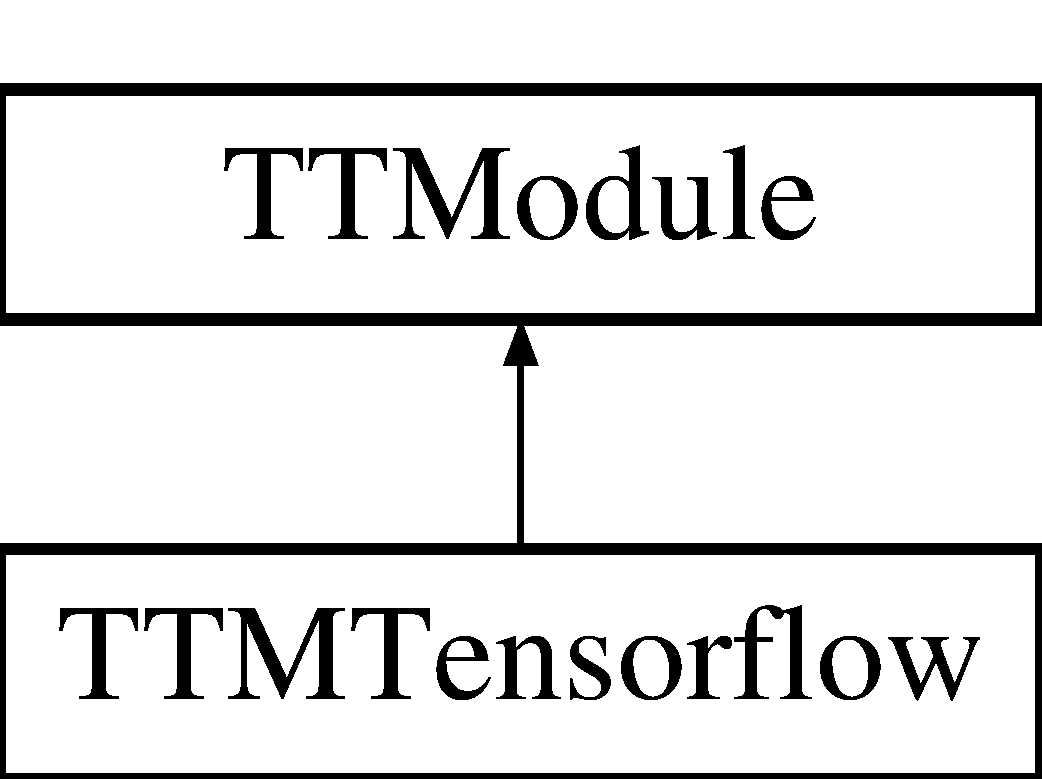
\includegraphics[height=2.000000cm]{classTTMTensorflow}
\end{center}
\end{figure}
\subsection*{Public Member Functions}
\begin{DoxyCompactItemize}
\item 
void \hyperlink{classTTMTensorflow_ae8a95bbecd4a21698b64dc95e99f5f0f}{get\-Parameters} (const \hyperlink{classcfg_1_1CfgDocument}{cfg\-::\-Cfg\-Document} $\ast$, const std\-::string \&)
\item 
void \hyperlink{classTTMTensorflow_afe5cdab757948e8eb2713fab0385869b}{run} (\hyperlink{classTopTaggerResults}{Top\-Tagger\-Results} \&)
\end{DoxyCompactItemize}
\subsection*{Additional Inherited Members}


\subsection{Detailed Description}
This module implements an interface to Tensorflow through the tensorflow c-\/api for filtering top candidates. This module places top candidates which pass the requirements directly into the final top list.


\begin{DoxyParams}{Parameters}
{\em disc\-Cut} & (float) Highest minimum discriminator threshold allowed (If disc\-Offest is set $>$ 1 and disc\-Slope is positive then this serves as a basic discriminator threshold) \\
\hline
{\em disc\-Offset} & (float) Discriminator cut for zero pt top candidates \\
\hline
{\em disc\-Slope} & (float) Pt dependent slopt for discriminator cut \\
\hline
{\em model\-File} & (string) Path to the model file \\
\hline
{\em N\-Constituents} & (int) Type of constituent to apply selection to (1 -\/ monojet, 2 -\/ dijet, 3 -\/ trijet) \\
\hline
{\em input\-Op} & (string) Input operation for the tensorflow graph \\
\hline
{\em output\-Op} & (string) Output operation of the tensorflow graph \\
\hline
{\em csv\-Threshold} & (float) Threshold on b-\/tag discriminator to be considered a b-\/jet. \\
\hline
{\em b\-Eta\-Cut} & (float) Requirment on $\vert$eta$\vert$ for a constituent to be considered a b-\/jet \\
\hline
{\em max\-Nb\-In\-Top} & (int) The maximum number of constituent jets which can be b-\/tagged for the candidate to be a final top (set $<$ 0 to disable) \\
\hline
{\em mva\-Var\mbox{[}$\,$\mbox{]}} & (string -\/ array) M\-V\-A variable input names \\
\hline
\end{DoxyParams}


\subsection{Member Function Documentation}
\hypertarget{classTTMTensorflow_ae8a95bbecd4a21698b64dc95e99f5f0f}{\index{T\-T\-M\-Tensorflow@{T\-T\-M\-Tensorflow}!get\-Parameters@{get\-Parameters}}
\index{get\-Parameters@{get\-Parameters}!TTMTensorflow@{T\-T\-M\-Tensorflow}}
\subsubsection[{get\-Parameters}]{\setlength{\rightskip}{0pt plus 5cm}void T\-T\-M\-Tensorflow\-::get\-Parameters (
\begin{DoxyParamCaption}
\item[{const {\bf cfg\-::\-Cfg\-Document} $\ast$}]{, }
\item[{const std\-::string \&}]{}
\end{DoxyParamCaption}
)\hspace{0.3cm}{\ttfamily [virtual]}}}\label{classTTMTensorflow_ae8a95bbecd4a21698b64dc95e99f5f0f}
This function is called by \hyperlink{classTopTagger}{Top\-Tagger} to configure each module based upon the information present in the configuration file. The inputs for this function are provided by \hyperlink{classTopTagger}{Top\-Tagger} and are the configuration document object and the local context string for this module. The local context string defines where to look in the configuration file for the local parameters. 

Implements \hyperlink{classTTModule_aa9d2842c9e94782059fe92044a68e3a6}{T\-T\-Module}.

\hypertarget{classTTMTensorflow_afe5cdab757948e8eb2713fab0385869b}{\index{T\-T\-M\-Tensorflow@{T\-T\-M\-Tensorflow}!run@{run}}
\index{run@{run}!TTMTensorflow@{T\-T\-M\-Tensorflow}}
\subsubsection[{run}]{\setlength{\rightskip}{0pt plus 5cm}void T\-T\-M\-Tensorflow\-::run (
\begin{DoxyParamCaption}
\item[{{\bf Top\-Tagger\-Results} \&}]{}
\end{DoxyParamCaption}
)\hspace{0.3cm}{\ttfamily [virtual]}}}\label{classTTMTensorflow_afe5cdab757948e8eb2713fab0385869b}
run is called automatically by \hyperlink{classTopTagger}{Top\-Tagger} once per event to run th emodule. The module interfaces with other modules through the \hyperlink{classTopTaggerResults}{Top\-Tagger\-Results} object which is passed as a non-\/const reference from \hyperlink{classTopTagger}{Top\-Tagger}. 

Implements \hyperlink{classTTModule_a14e7c03fbf4ee1a5008c9344adc7c896}{T\-T\-Module}.



The documentation for this class was generated from the following files\-:\begin{DoxyCompactItemize}
\item 
/home/travis/build/susy2015/\-Top\-Tagger/\-Top\-Tagger/interface/T\-T\-M\-Tensorflow.\-h\item 
/home/travis/build/susy2015/\-Top\-Tagger/\-Top\-Tagger/src/T\-T\-M\-Tensorflow.\-cpp\end{DoxyCompactItemize}

\hypertarget{classTTMTFPyBind}{\section{T\-T\-M\-T\-F\-Py\-Bind Class Reference}
\label{classTTMTFPyBind}\index{T\-T\-M\-T\-F\-Py\-Bind@{T\-T\-M\-T\-F\-Py\-Bind}}
}


{\ttfamily \#include $<$T\-T\-M\-T\-F\-Py\-Bind.\-h$>$}

Inheritance diagram for T\-T\-M\-T\-F\-Py\-Bind\-:\begin{figure}[H]
\begin{center}
\leavevmode
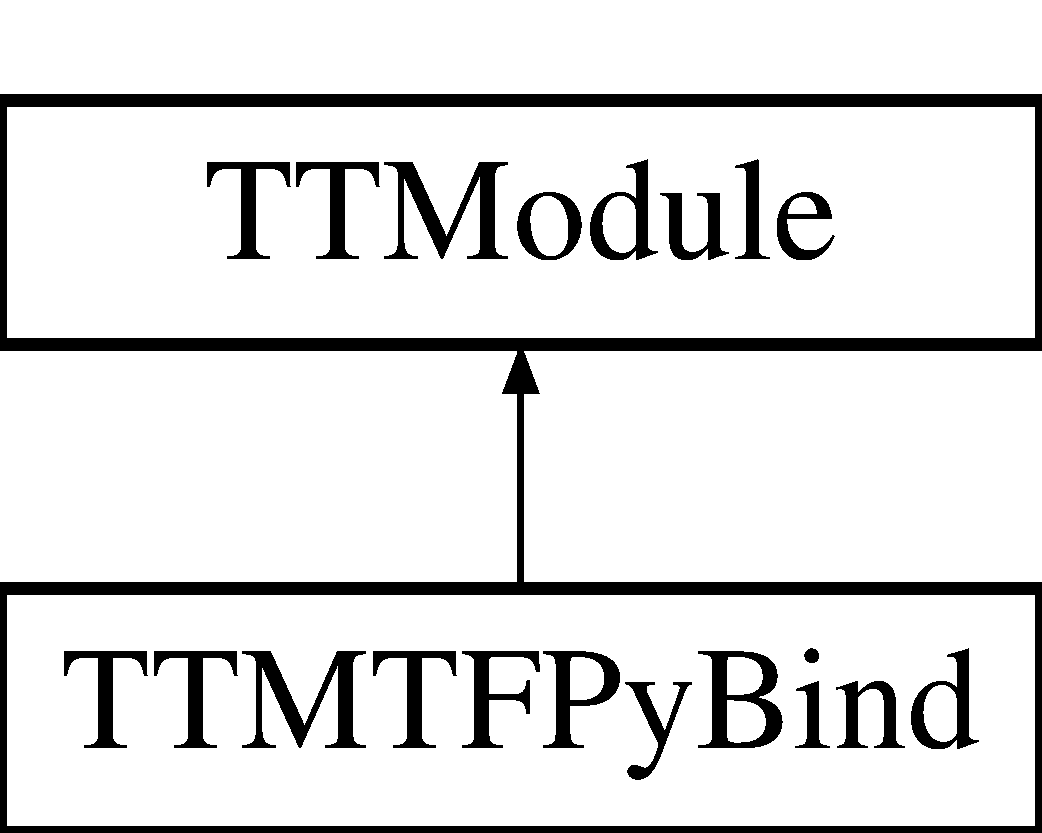
\includegraphics[height=2.000000cm]{classTTMTFPyBind}
\end{center}
\end{figure}
\subsection*{Public Member Functions}
\begin{DoxyCompactItemize}
\item 
void \hyperlink{classTTMTFPyBind_a3c9f2ca6bc095df3bad89c531cd45544}{get\-Parameters} (const \hyperlink{classcfg_1_1CfgDocument}{cfg\-::\-Cfg\-Document} $\ast$, const std\-::string \&)
\item 
void \hyperlink{classTTMTFPyBind_a5815a77655f5500c117cf71269105242}{run} (\hyperlink{classTopTaggerResults}{Top\-Tagger\-Results} \&)
\end{DoxyCompactItemize}


\subsection{Detailed Description}
This module implements an interface to Tensorflow through python for filtering top candidates. This module places top candidates which pass the requirements directly into the final top list.


\begin{DoxyParams}{Parameters}
{\em disc\-Cut} & (float) Highest minimum discriminator threshold allowed (If disc\-Offest is set $>$ 1 and disc\-Slope is positive then this serves as a basic discriminator threshold) \\
\hline
{\em disc\-Offset} & (float) Discriminator cut for zero pt top candidates \\
\hline
{\em disc\-Slope} & (float) Pt dependent slopt for discriminator cut \\
\hline
{\em model\-File} & (string) Path to the model file \\
\hline
{\em N\-Constituents} & (int) Type of constituent to apply selection to (1 -\/ monojet, 2 -\/ dijet, 3 -\/ trijet) \\
\hline
{\em input\-Op} & (string) Input operation for the tensorflow graph \\
\hline
{\em output\-Op} & (string) Output operation of the tensorflow graph \\
\hline
{\em csv\-Threshold} & (float) Threshold on b-\/tag discriminator to be considered a b-\/jet. \\
\hline
{\em b\-Eta\-Cut} & (float) Requirment on $\vert$eta$\vert$ for a constituent to be considered a b-\/jet \\
\hline
{\em max\-Nb\-In\-Top} & (int) The maximum number of constituent jets which can be b-\/tagged for the candidate to be a final top (set $<$ 0 to disable) \\
\hline
{\em mva\-Var\mbox{[}$\,$\mbox{]}} & (string -\/ array) M\-V\-A variable input names \\
\hline
\end{DoxyParams}


\subsection{Member Function Documentation}
\hypertarget{classTTMTFPyBind_a3c9f2ca6bc095df3bad89c531cd45544}{\index{T\-T\-M\-T\-F\-Py\-Bind@{T\-T\-M\-T\-F\-Py\-Bind}!get\-Parameters@{get\-Parameters}}
\index{get\-Parameters@{get\-Parameters}!TTMTFPyBind@{T\-T\-M\-T\-F\-Py\-Bind}}
\subsubsection[{get\-Parameters}]{\setlength{\rightskip}{0pt plus 5cm}void T\-T\-M\-T\-F\-Py\-Bind\-::get\-Parameters (
\begin{DoxyParamCaption}
\item[{const {\bf cfg\-::\-Cfg\-Document} $\ast$}]{, }
\item[{const std\-::string \&}]{}
\end{DoxyParamCaption}
)\hspace{0.3cm}{\ttfamily [virtual]}}}\label{classTTMTFPyBind_a3c9f2ca6bc095df3bad89c531cd45544}
This function is called by \hyperlink{classTopTagger}{Top\-Tagger} to configure each module based upon the information present in the configuration file. The inputs for this function are provided by \hyperlink{classTopTagger}{Top\-Tagger} and are the configuration document object and the local context string for this module. The local context string defines where to look in the configuration file for the local parameters. 

Implements \hyperlink{classTTModule_aa9d2842c9e94782059fe92044a68e3a6}{T\-T\-Module}.

\hypertarget{classTTMTFPyBind_a5815a77655f5500c117cf71269105242}{\index{T\-T\-M\-T\-F\-Py\-Bind@{T\-T\-M\-T\-F\-Py\-Bind}!run@{run}}
\index{run@{run}!TTMTFPyBind@{T\-T\-M\-T\-F\-Py\-Bind}}
\subsubsection[{run}]{\setlength{\rightskip}{0pt plus 5cm}void T\-T\-M\-T\-F\-Py\-Bind\-::run (
\begin{DoxyParamCaption}
\item[{{\bf Top\-Tagger\-Results} \&}]{}
\end{DoxyParamCaption}
)\hspace{0.3cm}{\ttfamily [virtual]}}}\label{classTTMTFPyBind_a5815a77655f5500c117cf71269105242}
run is called automatically by \hyperlink{classTopTagger}{Top\-Tagger} once per event to run th emodule. The module interfaces with other modules through the \hyperlink{classTopTaggerResults}{Top\-Tagger\-Results} object which is passed as a non-\/const reference from \hyperlink{classTopTagger}{Top\-Tagger}. 

Implements \hyperlink{classTTModule_a14e7c03fbf4ee1a5008c9344adc7c896}{T\-T\-Module}.



The documentation for this class was generated from the following files\-:\begin{DoxyCompactItemize}
\item 
/home/travis/build/susy2015/\-Top\-Tagger/\-Top\-Tagger/include/T\-T\-M\-T\-F\-Py\-Bind.\-h\item 
/home/travis/build/susy2015/\-Top\-Tagger/\-Top\-Tagger/src/T\-T\-M\-T\-F\-Py\-Bind.\-cpp\end{DoxyCompactItemize}

\hypertarget{classTTMTMVA}{\section{T\-T\-M\-T\-M\-V\-A Class Reference}
\label{classTTMTMVA}\index{T\-T\-M\-T\-M\-V\-A@{T\-T\-M\-T\-M\-V\-A}}
}


{\ttfamily \#include $<$T\-T\-M\-T\-M\-V\-A.\-h$>$}

Inheritance diagram for T\-T\-M\-T\-M\-V\-A\-:\begin{figure}[H]
\begin{center}
\leavevmode
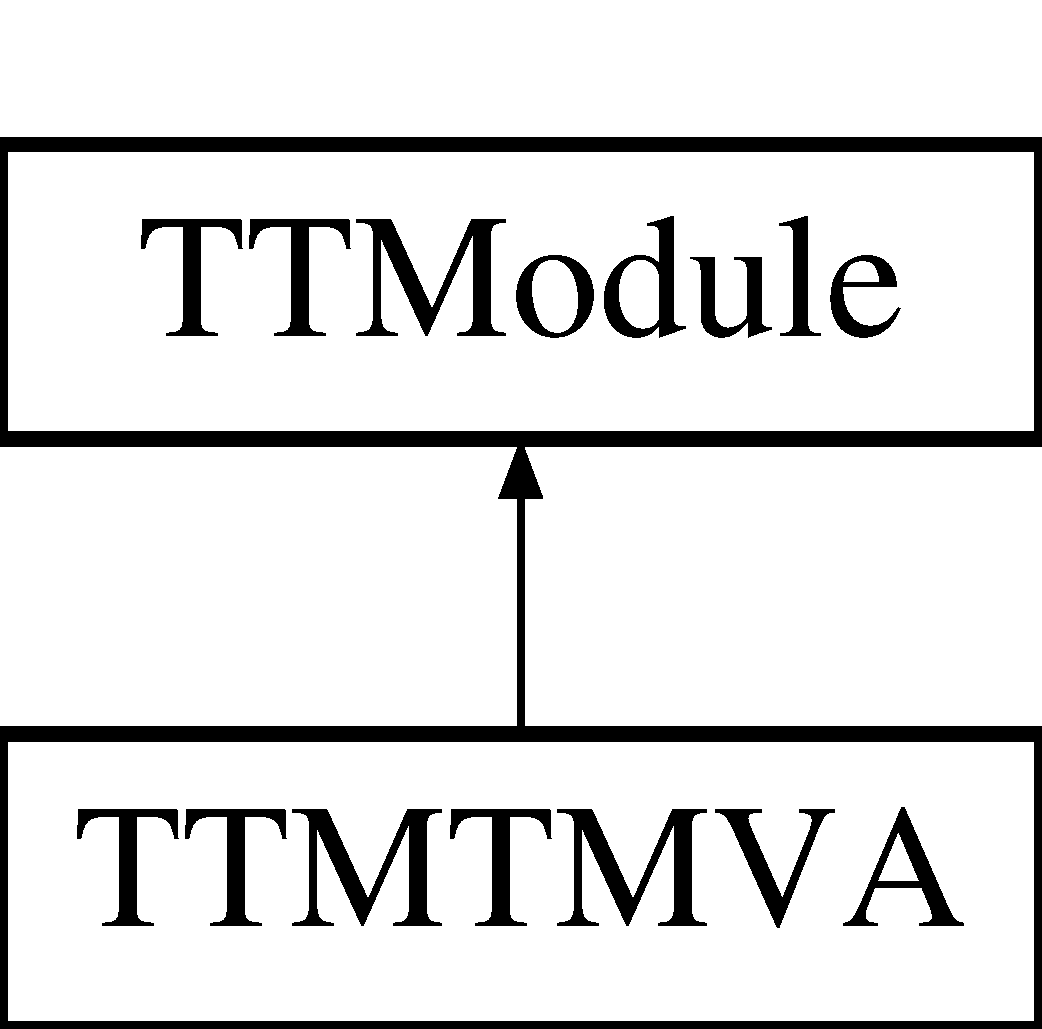
\includegraphics[height=2.000000cm]{classTTMTMVA}
\end{center}
\end{figure}
\subsection*{Public Member Functions}
\begin{DoxyCompactItemize}
\item 
void \hyperlink{classTTMTMVA_a00b1eda9a6425e95eb4e0f41688236e0}{get\-Parameters} (const \hyperlink{classcfg_1_1CfgDocument}{cfg\-::\-Cfg\-Document} $\ast$, const std\-::string \&)
\item 
void \hyperlink{classTTMTMVA_a640584674f072cb893685845080c5eb9}{run} (\hyperlink{classTopTaggerResults}{Top\-Tagger\-Results} \&)
\end{DoxyCompactItemize}
\subsection*{Additional Inherited Members}


\subsection{Detailed Description}
This module implements an interface to T\-M\-V\-A for filtering top candidates. This module can either pass entries directly into the final top list, or filter entries out of the final top list if they do not pass the selection criterion.


\begin{DoxyParams}{Parameters}
{\em disc\-Cut} & (float) Minimum threshold for the T\-M\-V\-A discriminator for te candidate to pass the selection \\
\hline
{\em model\-File} & (string) Path to the model file \\
\hline
{\em model\-Name} & (string) Name of the model \\
\hline
{\em N\-Constituents} & (int) What type of constituents to apply selection too (1 -\/ monojet, 2 -\/ dijet, 3 -\/ trijet) \\
\hline
{\em filter} & (bool) Filter failing candidates from the final top list instead of adding passing candidates to the final tops list \\
\hline
{\em mva\-Var\mbox{[}$\,$\mbox{]}} & (string -\/ array) M\-V\-A variable input names \\
\hline
\end{DoxyParams}


\subsection{Member Function Documentation}
\hypertarget{classTTMTMVA_a00b1eda9a6425e95eb4e0f41688236e0}{\index{T\-T\-M\-T\-M\-V\-A@{T\-T\-M\-T\-M\-V\-A}!get\-Parameters@{get\-Parameters}}
\index{get\-Parameters@{get\-Parameters}!TTMTMVA@{T\-T\-M\-T\-M\-V\-A}}
\subsubsection[{get\-Parameters}]{\setlength{\rightskip}{0pt plus 5cm}void T\-T\-M\-T\-M\-V\-A\-::get\-Parameters (
\begin{DoxyParamCaption}
\item[{const {\bf cfg\-::\-Cfg\-Document} $\ast$}]{, }
\item[{const std\-::string \&}]{}
\end{DoxyParamCaption}
)\hspace{0.3cm}{\ttfamily [virtual]}}}\label{classTTMTMVA_a00b1eda9a6425e95eb4e0f41688236e0}
This function is called by \hyperlink{classTopTagger}{Top\-Tagger} to configure each module based upon the information present in the configuration file. The inputs for this function are provided by \hyperlink{classTopTagger}{Top\-Tagger} and are the configuration document object and the local context string for this module. The local context string defines where to look in the configuration file for the local parameters. 

Implements \hyperlink{classTTModule_aa9d2842c9e94782059fe92044a68e3a6}{T\-T\-Module}.

\hypertarget{classTTMTMVA_a640584674f072cb893685845080c5eb9}{\index{T\-T\-M\-T\-M\-V\-A@{T\-T\-M\-T\-M\-V\-A}!run@{run}}
\index{run@{run}!TTMTMVA@{T\-T\-M\-T\-M\-V\-A}}
\subsubsection[{run}]{\setlength{\rightskip}{0pt plus 5cm}void T\-T\-M\-T\-M\-V\-A\-::run (
\begin{DoxyParamCaption}
\item[{{\bf Top\-Tagger\-Results} \&}]{}
\end{DoxyParamCaption}
)\hspace{0.3cm}{\ttfamily [virtual]}}}\label{classTTMTMVA_a640584674f072cb893685845080c5eb9}
run is called automatically by \hyperlink{classTopTagger}{Top\-Tagger} once per event to run th emodule. The module interfaces with other modules through the \hyperlink{classTopTaggerResults}{Top\-Tagger\-Results} object which is passed as a non-\/const reference from \hyperlink{classTopTagger}{Top\-Tagger}. 

Implements \hyperlink{classTTModule_a14e7c03fbf4ee1a5008c9344adc7c896}{T\-T\-Module}.



The documentation for this class was generated from the following files\-:\begin{DoxyCompactItemize}
\item 
/home/travis/build/susy2015/\-Top\-Tagger/\-Top\-Tagger/interface/T\-T\-M\-T\-M\-V\-A.\-h\item 
/home/travis/build/susy2015/\-Top\-Tagger/\-Top\-Tagger/src/T\-T\-M\-T\-M\-V\-A.\-cpp\end{DoxyCompactItemize}

\hypertarget{classTTMXGBoost}{\section{T\-T\-M\-X\-G\-Boost Class Reference}
\label{classTTMXGBoost}\index{T\-T\-M\-X\-G\-Boost@{T\-T\-M\-X\-G\-Boost}}
}


{\ttfamily \#include $<$T\-T\-M\-X\-G\-Boost.\-h$>$}

Inheritance diagram for T\-T\-M\-X\-G\-Boost\-:\begin{figure}[H]
\begin{center}
\leavevmode
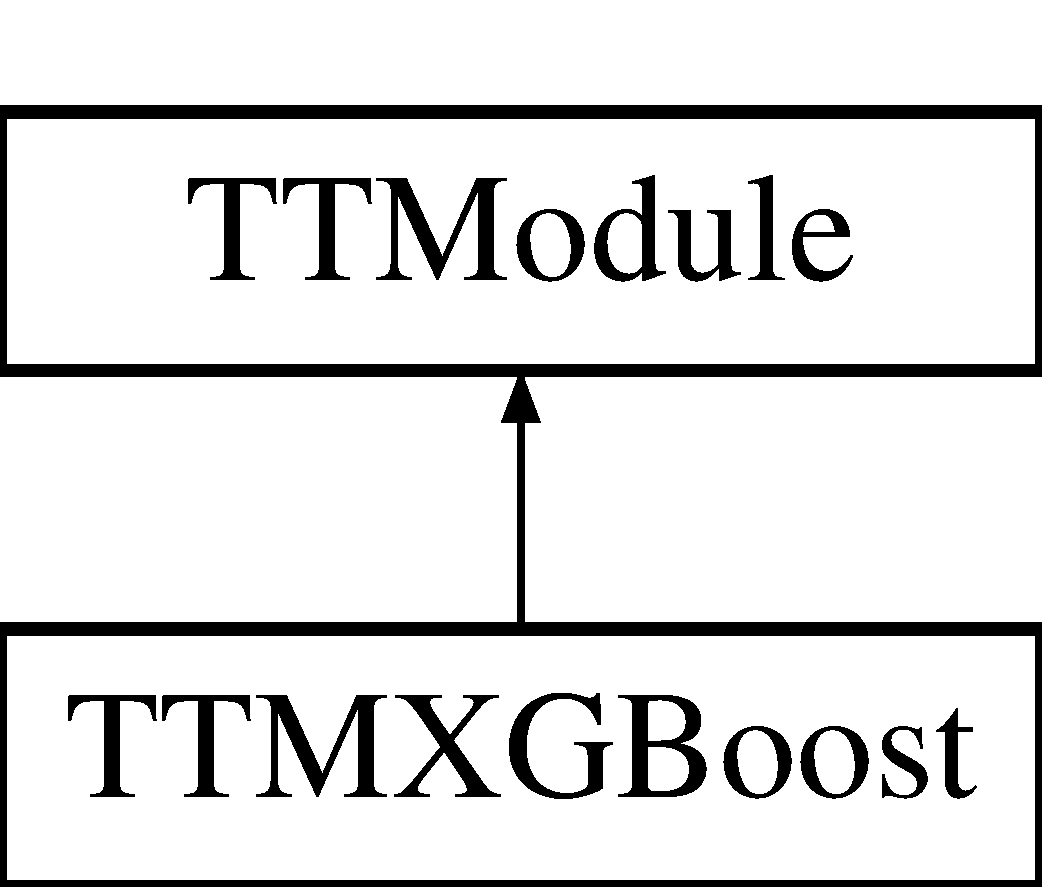
\includegraphics[height=2.000000cm]{classTTMXGBoost}
\end{center}
\end{figure}
\subsection*{Public Member Functions}
\begin{DoxyCompactItemize}
\item 
void \hyperlink{classTTMXGBoost_a852aba8afb6f453187871e232927e622}{get\-Parameters} (const \hyperlink{classcfg_1_1CfgDocument}{cfg\-::\-Cfg\-Document} $\ast$, const std\-::string \&)
\item 
void \hyperlink{classTTMXGBoost_afd522be937c0e1c8226c83cc6888c666}{run} (\hyperlink{classTopTaggerResults}{Top\-Tagger\-Results} \&)
\end{DoxyCompactItemize}
\subsection*{Additional Inherited Members}


\subsection{Detailed Description}
This module implements an interface to the Open\-C\-V randomforest package for filtering top candidates. This module can either pass entries directly into the final top list, or filter entries out of the final top list if they do not pass the selection criteria.


\begin{DoxyParams}{Parameters}
{\em disc\-Cut} & (float) Minimum threshold for the T\-M\-V\-A discriminator for the candidate to pass the selection \\
\hline
{\em model\-File} & (string) Path to the model file \\
\hline
{\em N\-Constituents} & (int) Category of top to apply selection too (1 -\/ monojet, 2 -\/ dijet, 3 -\/ trijet) \\
\hline
{\em N\-Cores} & (int) Number of cpu to allow X\-G\-Boost to use (default 1) \\
\hline
{\em csv\-Threshold} & (float) Threshold on b-\/tag discriminator to be considered a b-\/jet. \\
\hline
{\em b\-Eta\-Cut} & (float) Requirment on $\vert$eta$\vert$ for a constituent to be considered a b-\/jet \\
\hline
{\em max\-Nb\-In\-Top} & (int) The maximum number of constituent jets which can be b-\/tagged for the candidate to be a final $\ast$\\
\hline
{\em mva\-Var\mbox{[}$\,$\mbox{]}} & (string -\/ array) M\-V\-A variable input names \\
\hline
\end{DoxyParams}


\subsection{Member Function Documentation}
\hypertarget{classTTMXGBoost_a852aba8afb6f453187871e232927e622}{\index{T\-T\-M\-X\-G\-Boost@{T\-T\-M\-X\-G\-Boost}!get\-Parameters@{get\-Parameters}}
\index{get\-Parameters@{get\-Parameters}!TTMXGBoost@{T\-T\-M\-X\-G\-Boost}}
\subsubsection[{get\-Parameters}]{\setlength{\rightskip}{0pt plus 5cm}void T\-T\-M\-X\-G\-Boost\-::get\-Parameters (
\begin{DoxyParamCaption}
\item[{const {\bf cfg\-::\-Cfg\-Document} $\ast$}]{, }
\item[{const std\-::string \&}]{}
\end{DoxyParamCaption}
)\hspace{0.3cm}{\ttfamily [virtual]}}}\label{classTTMXGBoost_a852aba8afb6f453187871e232927e622}
This function is called by \hyperlink{classTopTagger}{Top\-Tagger} to configure each module based upon the information present in the configuration file. The inputs for this function are provided by \hyperlink{classTopTagger}{Top\-Tagger} and are the configuration document object and the local context string for this module. The local context string defines where to look in the configuration file for the local parameters. 

Implements \hyperlink{classTTModule_aa9d2842c9e94782059fe92044a68e3a6}{T\-T\-Module}.

\hypertarget{classTTMXGBoost_afd522be937c0e1c8226c83cc6888c666}{\index{T\-T\-M\-X\-G\-Boost@{T\-T\-M\-X\-G\-Boost}!run@{run}}
\index{run@{run}!TTMXGBoost@{T\-T\-M\-X\-G\-Boost}}
\subsubsection[{run}]{\setlength{\rightskip}{0pt plus 5cm}void T\-T\-M\-X\-G\-Boost\-::run (
\begin{DoxyParamCaption}
\item[{{\bf Top\-Tagger\-Results} \&}]{}
\end{DoxyParamCaption}
)\hspace{0.3cm}{\ttfamily [virtual]}}}\label{classTTMXGBoost_afd522be937c0e1c8226c83cc6888c666}
run is called automatically by \hyperlink{classTopTagger}{Top\-Tagger} once per event to run th emodule. The module interfaces with other modules through the \hyperlink{classTopTaggerResults}{Top\-Tagger\-Results} object which is passed as a non-\/const reference from \hyperlink{classTopTagger}{Top\-Tagger}. 

Implements \hyperlink{classTTModule_a14e7c03fbf4ee1a5008c9344adc7c896}{T\-T\-Module}.



The documentation for this class was generated from the following files\-:\begin{DoxyCompactItemize}
\item 
/home/travis/build/susy2015/\-Top\-Tagger/\-Top\-Tagger/interface/T\-T\-M\-X\-G\-Boost.\-h\item 
/home/travis/build/susy2015/\-Top\-Tagger/\-Top\-Tagger/src/T\-T\-M\-X\-G\-Boost.\-cpp\end{DoxyCompactItemize}

\hypertarget{classhcalcfg_1_1UTF8Buffer}{\section{hcalcfg\-:\-:U\-T\-F8\-Buffer Class Reference}
\label{classhcalcfg_1_1UTF8Buffer}\index{hcalcfg\-::\-U\-T\-F8\-Buffer@{hcalcfg\-::\-U\-T\-F8\-Buffer}}
}
Inheritance diagram for hcalcfg\-:\-:U\-T\-F8\-Buffer\-:\begin{figure}[H]
\begin{center}
\leavevmode
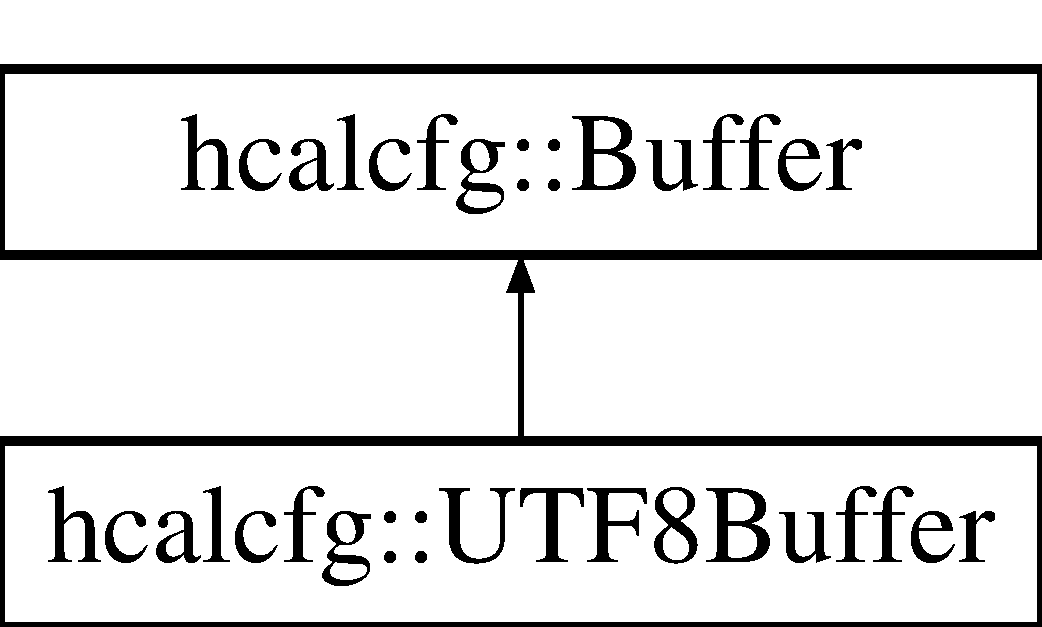
\includegraphics[height=2.000000cm]{classhcalcfg_1_1UTF8Buffer}
\end{center}
\end{figure}
\subsection*{Public Member Functions}
\begin{DoxyCompactItemize}
\item 
\hypertarget{classhcalcfg_1_1UTF8Buffer_aa202be6b47eeb2471d0eda588f1293ce}{{\bfseries U\-T\-F8\-Buffer} (\hyperlink{classhcalcfg_1_1Buffer}{Buffer} $\ast$b)}\label{classhcalcfg_1_1UTF8Buffer_aa202be6b47eeb2471d0eda588f1293ce}

\item 
\hypertarget{classhcalcfg_1_1UTF8Buffer_a14144ddafb52089c447cf50c89ae4466}{virtual int {\bfseries Read} ()}\label{classhcalcfg_1_1UTF8Buffer_a14144ddafb52089c447cf50c89ae4466}

\end{DoxyCompactItemize}
\subsection*{Additional Inherited Members}


The documentation for this class was generated from the following files\-:\begin{DoxyCompactItemize}
\item 
/home/travis/build/susy2015/\-Top\-Tagger/\-Cfg\-Parser/include/Scanner.\-h\item 
/home/travis/build/susy2015/\-Top\-Tagger/\-Cfg\-Parser/src/Scanner.\-cpp\end{DoxyCompactItemize}

\chapter{File Documentation}
\hypertarget{TopTaggerUtilities_8h}{\section{/home/travis/build/susy2015/\-Top\-Tagger/\-Top\-Tagger/interface/\-Top\-Tagger\-Utilities.h File Reference}
\label{TopTaggerUtilities_8h}\index{/home/travis/build/susy2015/\-Top\-Tagger/\-Top\-Tagger/interface/\-Top\-Tagger\-Utilities.\-h@{/home/travis/build/susy2015/\-Top\-Tagger/\-Top\-Tagger/interface/\-Top\-Tagger\-Utilities.\-h}}
}
{\ttfamily \#include $<$vector$>$}\\*
{\ttfamily \#include $<$map$>$}\\*
{\ttfamily \#include $<$string$>$}\\*
{\ttfamily \#include \char`\"{}Top\-Tagger/\-Top\-Tagger/interface/\-Constituent.\-h\char`\"{}}\\*
{\ttfamily \#include \char`\"{}Top\-Tagger/\-Cfg\-Parser/include/\-T\-T\-Exception.\-h\char`\"{}}\\*
{\ttfamily \#include \char`\"{}T\-F1.\-h\char`\"{}}\\*
{\ttfamily \#include \char`\"{}T\-File.\-h\char`\"{}}\\*
{\ttfamily \#include \char`\"{}T\-Lorentz\-Vector.\-h\char`\"{}}\\*
{\ttfamily \#include \char`\"{}Math/\-Vector\-Util.\-h\char`\"{}}\\*
\subsection*{Classes}
\begin{DoxyCompactItemize}
\item 
class \hyperlink{classttUtility_1_1ConstGenInputs}{tt\-Utility\-::\-Const\-Gen\-Inputs}
\item 
class \hyperlink{classttUtility_1_1ConstAK4Inputs}{tt\-Utility\-::\-Const\-A\-K4\-Inputs$<$ F\-L\-O\-A\-T\-T\-Y\-P\-E, F\-L\-O\-A\-T\-C\-O\-N\-T\-A\-I\-N\-E\-R\-T\-Y\-P\-E, L\-O\-R\-E\-N\-T\-Z\-V\-E\-C\-T\-O\-R\-C\-O\-N\-T\-A\-I\-N\-E\-R, I\-N\-T\-C\-O\-N\-T\-A\-I\-N\-E\-R\-T\-Y\-P\-E $>$}
\item 
class \hyperlink{classttUtility_1_1ConstAK8Inputs}{tt\-Utility\-::\-Const\-A\-K8\-Inputs$<$ F\-L\-O\-A\-T\-T\-Y\-P\-E, F\-L\-O\-A\-T\-C\-O\-N\-T\-A\-I\-N\-E\-R\-T\-Y\-P\-E, L\-O\-R\-E\-N\-T\-Z\-V\-E\-C\-T\-O\-R\-C\-O\-N\-T\-A\-I\-N\-E\-R $>$}
\item 
class \hyperlink{classttUtility_1_1ConstResolvedCandInputs}{tt\-Utility\-::\-Const\-Resolved\-Cand\-Inputs$<$ F\-L\-O\-A\-T\-T\-Y\-P\-E, F\-L\-O\-A\-T\-C\-O\-N\-T\-A\-I\-N\-E\-R\-T\-Y\-P\-E, I\-N\-T\-C\-O\-N\-T\-A\-I\-N\-E\-R\-T\-Y\-P\-E, L\-O\-R\-E\-N\-T\-Z\-V\-E\-C\-T\-O\-R\-C\-O\-N\-T\-A\-I\-N\-E\-R $>$}
\item 
class \hyperlink{classttUtility_1_1MVAInputCalculator}{tt\-Utility\-::\-M\-V\-A\-Input\-Calculator}
\item 
class \hyperlink{classttUtility_1_1BDTMonojetInputCalculator}{tt\-Utility\-::\-B\-D\-T\-Monojet\-Input\-Calculator}
\item 
class \hyperlink{classttUtility_1_1BDTDijetInputCalculator}{tt\-Utility\-::\-B\-D\-T\-Dijet\-Input\-Calculator}
\item 
class \hyperlink{classttUtility_1_1TrijetInputCalculator}{tt\-Utility\-::\-Trijet\-Input\-Calculator}
\end{DoxyCompactItemize}
\subsection*{Functions}
\begin{DoxyCompactItemize}
\item 
\hypertarget{namespacettUtility_a2b026c6cf169e2c1554b51b3c095cf2b}{{\footnotesize template$<$typename T , typename... Args$>$ }\\void {\bfseries tt\-Utility\-::package\-Constituents\-Recurse} (std\-::vector$<$ \hyperlink{classConstituent}{Constituent} $>$ \&constituents, T input, Args...\-args)}\label{namespacettUtility_a2b026c6cf169e2c1554b51b3c095cf2b}

\begin{DoxyCompactList}\small\item\em Resurcive function to assemble constituents from arbitrary list of input classes. Don't call this function! \end{DoxyCompactList}\item 
\hypertarget{namespacettUtility_a81539600933a20ad472d9cdc3061266a}{{\footnotesize template$<$typename T $>$ }\\void {\bfseries tt\-Utility\-::package\-Constituents\-Recurse} (std\-::vector$<$ \hyperlink{classConstituent}{Constituent} $>$ \&constituents, T input)}\label{namespacettUtility_a81539600933a20ad472d9cdc3061266a}

\begin{DoxyCompactList}\small\item\em recursion termimnation specialization. Don't call this function! \end{DoxyCompactList}\item 
\hypertarget{namespacettUtility_afe8c7a2d46380c2f4d17d1ac0d140571}{{\footnotesize template$<$typename... Args$>$ }\\std\-::vector$<$ \hyperlink{classConstituent}{Constituent} $>$ {\bfseries tt\-Utility\-::package\-Constituents} (Args...\-args)}\label{namespacettUtility_afe8c7a2d46380c2f4d17d1ac0d140571}

\begin{DoxyCompactList}\small\item\em Function to fill constituent list based upon arbitrary list of input objects. \end{DoxyCompactList}\item 
\hypertarget{namespacettUtility_abea3ec7286f12e4786567d7c83ecc47f}{std\-::vector$<$ \hyperlink{classConstituent}{Constituent} $>$ {\bfseries tt\-Utility\-::package\-Constituents\-A\-K4} (Const\-A\-K4\-Inputs$<$ float $>$ \&inputs)}\label{namespacettUtility_abea3ec7286f12e4786567d7c83ecc47f}

\begin{DoxyCompactList}\small\item\em Python compatibility function. \end{DoxyCompactList}\item 
\hypertarget{namespacettUtility_af895527e07e2dc4f5a9b275aa20965d3}{std\-::vector$<$ \hyperlink{classConstituent}{Constituent} $>$ {\bfseries tt\-Utility\-::package\-Constituents} (const std\-::vector$<$ T\-Lorentz\-Vector $>$ \&jets\-L\-Vec, const std\-::vector$<$ double $>$ \&btag\-Factors, const std\-::vector$<$ double $>$ \&qg\-Likelihood)}\label{namespacettUtility_af895527e07e2dc4f5a9b275aa20965d3}

\begin{DoxyCompactList}\small\item\em backwards compatability overload \end{DoxyCompactList}\item 
\hypertarget{namespacettUtility_af52621678213f55c02a51ed2c271c9ec}{double {\bfseries tt\-Utility\-::calculate\-M\-T2} (const \hyperlink{classTopTaggerResults}{Top\-Tagger\-Results} \&ttr, const T\-Lorentz\-Vector \&met\-L\-Vec)}\label{namespacettUtility_af52621678213f55c02a51ed2c271c9ec}

\begin{DoxyCompactList}\small\item\em Tool to calcualte M\-T2 from tagger results. \end{DoxyCompactList}\item 
\hypertarget{namespacettUtility_a252b0369e36d8435119de4651c4c4427}{double {\bfseries tt\-Utility\-::core\-M\-T2calc} (const T\-Lorentz\-Vector \&fat\-Jet1\-L\-Vec, const T\-Lorentz\-Vector \&fat\-Jet2\-L\-Vec, const T\-Lorentz\-Vector \&met\-L\-Vec)}\label{namespacettUtility_a252b0369e36d8435119de4651c4c4427}

\item 
\hypertarget{namespacettUtility_a6b84aa7ccd9d2f792a232cf93fc4a8d1}{std\-::vector$<$ std\-::string $>$ {\bfseries tt\-Utility\-::get\-M\-V\-A\-Vars} ()}\label{namespacettUtility_a6b84aa7ccd9d2f792a232cf93fc4a8d1}

\item 
\hypertarget{namespacettUtility_ac068b841fc333960cddfe5dc270ebb4c}{bool {\bfseries tt\-Utility\-::rec\-Mom\-Search} (int start\-Index, int target\-Index, const std\-::vector$<$ int $>$ \&gen\-Decay\-Mom\-Idx\-Vec)}\label{namespacettUtility_ac068b841fc333960cddfe5dc270ebb4c}

\item 
\hypertarget{namespacettUtility_ab0b2e971158a9203b97f7d019c247d7e}{std\-::pair$<$ std\-::vector\\*
$<$ T\-Lorentz\-Vector $>$\\*
, std\-::vector$<$ std\-::vector\\*
$<$ const T\-Lorentz\-Vector $\ast$ $>$ $>$ $>$ {\bfseries tt\-Utility\-::\-Get\-Topdau\-Gen\-L\-Vec\-From\-Nano} (const std\-::vector$<$ T\-Lorentz\-Vector $>$ \&gen\-Decay\-L\-Vec, const std\-::vector$<$ int $>$ \&gen\-Decay\-Pdg\-Id\-Vec, const std\-::vector$<$ int $>$ \&gen\-Decay\-Stat\-Flag, const std\-::vector$<$ int $>$ \&gen\-Decay\-Mom\-Idx\-Vec)}\label{namespacettUtility_ab0b2e971158a9203b97f7d019c247d7e}

\item 
\hypertarget{namespacettUtility_a0497406d35fac347b288d37aa55c71e2}{std\-::vector$<$ T\-Lorentz\-Vector $>$ {\bfseries tt\-Utility\-::\-Get\-Had\-Top\-L\-Vec} (const std\-::vector$<$ T\-Lorentz\-Vector $>$ \&gen\-Decay\-L\-Vec, const std\-::vector$<$ int $>$ \&gen\-Decay\-Pdg\-Id\-Vec, const std\-::vector$<$ int $>$ \&gen\-Decay\-Idx\-Vec, const std\-::vector$<$ int $>$ \&gen\-Decay\-Mom\-Idx\-Vec)}\label{namespacettUtility_a0497406d35fac347b288d37aa55c71e2}

\begin{DoxyCompactList}\small\item\em Helper function to help find the hadronically decaying gen tops. \end{DoxyCompactList}\item 
\hypertarget{namespacettUtility_ab836e0b87270859faba59ee5a8e883ce}{std\-::vector$<$ const \\*
T\-Lorentz\-Vector $\ast$ $>$ {\bfseries tt\-Utility\-::\-Get\-Topdau\-L\-Vec} (const T\-Lorentz\-Vector \&top, const std\-::vector$<$ T\-Lorentz\-Vector $>$ \&gen\-Decay\-L\-Vec, const std\-::vector$<$ int $>$ \&gen\-Decay\-Pdg\-Id\-Vec, const std\-::vector$<$ int $>$ \&gen\-Decay\-Idx\-Vec, const std\-::vector$<$ int $>$ \&gen\-Decay\-Mom\-Idx\-Vec)}\label{namespacettUtility_ab836e0b87270859faba59ee5a8e883ce}

\begin{DoxyCompactList}\small\item\em Helper function to get the direct decay products of the gen tops. \end{DoxyCompactList}\item 
\hypertarget{namespacettUtility_aec20f7d06fde705bcc06211b74c8c227}{void {\bfseries tt\-Utility\-::auto\-Expand\-Environment\-Variables} (std\-::string \&)}\label{namespacettUtility_aec20f7d06fde705bcc06211b74c8c227}

\end{DoxyCompactItemize}

\hypertarget{TTModule_8h}{\section{/home/travis/build/susy2015/\-Top\-Tagger/\-Top\-Tagger/interface/\-T\-T\-Module.h File Reference}
\label{TTModule_8h}\index{/home/travis/build/susy2015/\-Top\-Tagger/\-Top\-Tagger/interface/\-T\-T\-Module.\-h@{/home/travis/build/susy2015/\-Top\-Tagger/\-Top\-Tagger/interface/\-T\-T\-Module.\-h}}
}
{\ttfamily \#include \char`\"{}Top\-Tagger/\-Top\-Tagger/interface/\-T\-T\-M\-Factory.\-h\char`\"{}}\\*
{\ttfamily \#include $<$functional$>$}\\*
\subsection*{Classes}
\begin{DoxyCompactItemize}
\item 
class \hyperlink{classTTModule}{T\-T\-Module}
\end{DoxyCompactItemize}
\subsection*{Macros}
\begin{DoxyCompactItemize}
\item 
\hypertarget{TTModule_8h_a503a61d6a681bacd3074975a6402d0cc}{\#define {\bfseries T\-T\-\_\-\-V\-A\-R\-I\-A\-B\-L\-E\-\_\-\-I\-S\-\_\-\-N\-O\-T\-\_\-\-U\-S\-E\-D}}\label{TTModule_8h_a503a61d6a681bacd3074975a6402d0cc}

\item 
\#define \hyperlink{TTModule_8h_a5aff241e827824ffd2c2efc4c5bf1fda}{R\-E\-G\-I\-S\-T\-E\-R\-\_\-\-T\-T\-M\-O\-D\-U\-L\-E}(\-\_\-module)~static bool T\-T\-\_\-\-V\-A\-R\-I\-A\-B\-L\-E\-\_\-\-I\-S\-\_\-\-N\-O\-T\-\_\-\-U\-S\-E\-D \-\_\-module \#\# \-\_\-module\-\_\-created = \hyperlink{classTTMFactory_a4651a7e0c90b7c36acbdada8de05a4b4}{T\-T\-M\-Factory\-::register\-Module}( \#\-\_\-module, \mbox{[}$\,$\mbox{]}()-\/$>$\hyperlink{classTTModule}{T\-T\-Module}$\ast$\{ return new \-\_\-module(); \} )
\end{DoxyCompactItemize}


\subsection{Macro Definition Documentation}
\hypertarget{TTModule_8h_a5aff241e827824ffd2c2efc4c5bf1fda}{\index{T\-T\-Module.\-h@{T\-T\-Module.\-h}!R\-E\-G\-I\-S\-T\-E\-R\-\_\-\-T\-T\-M\-O\-D\-U\-L\-E@{R\-E\-G\-I\-S\-T\-E\-R\-\_\-\-T\-T\-M\-O\-D\-U\-L\-E}}
\index{R\-E\-G\-I\-S\-T\-E\-R\-\_\-\-T\-T\-M\-O\-D\-U\-L\-E@{R\-E\-G\-I\-S\-T\-E\-R\-\_\-\-T\-T\-M\-O\-D\-U\-L\-E}!TTModule.h@{T\-T\-Module.\-h}}
\subsubsection[{R\-E\-G\-I\-S\-T\-E\-R\-\_\-\-T\-T\-M\-O\-D\-U\-L\-E}]{\setlength{\rightskip}{0pt plus 5cm}\#define R\-E\-G\-I\-S\-T\-E\-R\-\_\-\-T\-T\-M\-O\-D\-U\-L\-E(
\begin{DoxyParamCaption}
\item[{}]{\-\_\-module}
\end{DoxyParamCaption}
)~static bool T\-T\-\_\-\-V\-A\-R\-I\-A\-B\-L\-E\-\_\-\-I\-S\-\_\-\-N\-O\-T\-\_\-\-U\-S\-E\-D \-\_\-module \#\# \-\_\-module\-\_\-created = {\bf T\-T\-M\-Factory\-::register\-Module}( \#\-\_\-module, \mbox{[}$\,$\mbox{]}()-\/$>${\bf T\-T\-Module}$\ast$\{ return new \-\_\-module(); \} )}}\label{TTModule_8h_a5aff241e827824ffd2c2efc4c5bf1fda}
Magic macro for registering classes with the factory object. Every module definition must contain the line \char`\"{}\-R\-E\-G\-I\-S\-T\-E\-R\-\_\-\-T\-T\-M\-O\-D\-U\-L\-E(\-Module\-Class\-Name);\char`\"{}. 
%--- End generated contents ---

% Index
\newpage
\phantomsection
\addcontentsline{toc}{chapter}{Index}
\printindex

\end{document}
